%\documentclass[american,titlepage]{ntnuthesis}        % with extra blank pages
\documentclass[american,titlepage,oneside]{ntnuthesis} % without extra blank pages

% Used to make verbatim environment wrap lines
\usepackage{minted}
\usepackage{graphicx}


\title{Backup Architecture Resistant to Ransomware Attacks}
\shorttitle{Ransomware-Resistant Backup}
\author{Torstein Martinsheimen Egge \and Åsmund Hunderi Stemland  \and Omer Jonuzi}
\shortauthor{T. M. Egge \and O. Jonuzi \and Å. H. Stemland}
\date{\today} 

\addbibresource{thesis.bib}


% From https://www.overleaf.com/learn/latex/Glossaries

\makeglossaries % Prepare for adding glossary entries

\newglossaryentry{backup}
{
        name=backup,
        description={Copy of data that can be used to restore the original in case something happens to it.}
}

\newglossaryentry{exfiltration}
{
        name=data exfiltration,
        description={Transferring data out of an organization's network. Essentially data theft.}
}

\newglossaryentry{zero-day}
{
        name=zero-day,
        description={Computer security vulnerability that is unknown or unpatched.}
}

\newglossaryentry{malware}
{
        name=malware,
        description={Malicious software. General term for software that does damage to computers, IT systems, etc.}
}

\newglossaryentry{ransomware}
{
        name=ransomware,
        description={Type of malware that encrypts files, in order for the attacker to demand a ransom from their victims in exchange for the files being decrypted.}
}

\newglossaryentry{privilege escalation}
{
        name=privilege escalation,
        description={Attack where the attacker obtains unauthorized privileges/permissions, often by exploiting a vulnerability.}
}

\newglossaryentry{security controls}
{
        name=security controls,
        description={Noe her?}
}


\newglossaryentry{vm}
{
        name=VM,
        description={Short for Virtual Machine, a computer emulated in software.}
}

\newglossaryentry{OS}
{
        name=operating system,
        description={Software that manages hardware and provides services for users to interact with said hardware.}
}

\newglossaryentry{rdp}
{
        name=RDP,
        description={Remote Desktop Protocol. A Microsoft protocol for accessing computers via a graphical user interface remotely (over a network)}
}

\newglossaryentry{rsv}
{
        name=RSV,
        description={Recovery Services vault. A container for backup items and configurations in Azure}
}

\newglossaryentry{unmanaged}
{
        name=unmanaged service,
        description={When referring to cloud services, an unmanaged service is a service that is configured and maintained by the customer, and not by the cloud provider.}
}


% entries below are kept for reference

\newglossaryentry{bibliography}
{
        name=bibliography,
        plural=bibliographies,
        description={A list of the books referred to in a scholarly work,
typically printed as an appendix}
}

\newglossaryentry{maths}
{
    name=mathematics,
    description={Mathematics is what mathematicians do}
}


% --------------------
% ----- Acronyms -----
% --------------------

\newacronym{phd}{PhD}{philosophiae doctor}
\newacronym{CoPCSE}{CoPCSE@NTNU}{Community of Practice in Computer ScienceEducation at NTNU}
\newacronym{gcd}{GCD}{Greatest Common Divisor}
\newacronym{C&C}{C&C}{Command-and-control}
%\newacronym{rdp}{RDP}{Remote Desktop Protocol}
 % add glossary and acronym lists before document

\begin{document}

\chapter*{Abstract}

Ransomware attacks have been on the rise globally the last few years. They pose a serious threat to any business's data, reputation and operational capability.
Backups are an essential part of an effective strategy against ransomware attacks, 
functioning as the last line of defense.
Thus; how do you prevent a hacker from corrupting or outright deleting your backups 
before unleashing their ransomware?

In this thesis, we attempt to find the trends and characteristics that define modern ransomware,
as well as how to recover from modern ransomware attacks.
We explore various backup solutions for managed and unmanaged 
databases in Azure, the cloud service platform operated by Microsoft, and evaluate their effectiveness against modern ransomware attacks.
In addition, we look at security mechanisms and features in Azure that can help defend
backups from malicious actions.

The results address several security features which block a number of attack vectors. Furthermore, issues with the existing backup solutions are highlighted and in some cases suggestions for improvement proposed.
\chapter*{Sammendrag}
Løsepengevirusangrep har sett en økning globalt de siste årene. De representerer en alvorlig trussel mot enhver bedrifts data, omdømme og operasjonelle kapabiliteter. Sikkerhetskopier er en essensiell del av en effektiv strategi for å motså løsepengevirus-angrep, med funksjonen til en siste forsvarslinje. Dermed; Hvordan skal en hindre en hacker fra å infisere eller slette sikkerhetskopier før de setter i gang med løsepengevirus-angrepet?

I denne oppgaven forsøker vi å se på de trender og karakteristiske preg som definerer moderne løsepengevirus, i tillegg til hvordan gjenopprettelse etter et moderne løsepengevirus-angrep utspiller. Vi utforsker løsninger for sikkerhetskopiering av både administrerte og ikke-administrerte databaser på Azure, Microsoft sin plattform for skytjenester, og sammenligner hvor effektive de løsningene er på å motstå moderne løsepengevirus. I tillegg ser vi på sikkerhetsmekanismer og funksjoner i Azure som bidrar til sikring av backup mot ondsinnede handlinger.
Resultatene tar for seg flere sikkerhetsfunksjoner som setter en stopper for en rekke angrepsvektorer. Videre fremhever vi problemer knyttet til eksisterende backupløsninger og i noen tilfeller foreslår vi forbedringer. 

%Skriv norsk sammendragmer
%Ransomware attacks have been on the rise globally the last few years. They pose a serious threat to any business’s data, reputation and operational capability. Back- ups are an essential part of an effective strategy against ransomware attacks, functioning as the last line of defense.But how do you prevent a hacker from corrupt- ing or outright deleting your backups before unleashing their ransomware?

%In this thesis, we attempt to find the trends and characteristics that define modern ransomware, as well as how to recover from modern ransomware attacks. We explore various backup solutions for managed and unmanaged databases in Azure, the cloud computing service operated by Microsoft, and evaluate their ef- fectiveness against modern ransomware attacks. 

%In addition, we look at security mechanisms and features in Azure that can help defend backups from malicious actions. The results address several security features which block a number of attack vectors. Furthermore, issues with the existing backup solutions are highlighted and in some cases suggestions for improvement proposed. 

\tableofcontents
\listoffigures
% \listoftables
% \lstlistoflistings %commented out since we don't have any listings large enough to include at the start

\printglossary[type=\acronymtype] % Print acronyms
\printglossary                    % Print glossary

\chapter*{Preface}
This thesis was written as the final assignment of our bachelors degree in digital infrastructure and cybersecurity. It explores the cross-section between infrastructure and security: Security controls against ransomware in databases hosted in a public cloud environment.

We were motivated to write this thesis because we felt it was both relevant and important to organisations facing the growing threat of ransomware. No other theme has been as prevalent in cybersecurity news during our degree. The choice to focus on cloud environments is both relevant for today, but will remain relevant for years to come as well.

We hope this thesis is relevant to organisations unsure of how to assess the myriad of security features in cloud environments, and help them stay secure. 

We would like to thank TrønderEnergi for help with the project, NTNU for the opportunity to study relevant and important subjects. We would also like to thank our advisors: Helge Hafting, Gleb Sizov, and Joakim Klemets. All your advice helped us greatly. 
\chapter{Introduction}

\section{Background}
Ransomware is one of the biggest cyber threat businesses and organisations face today \cite{hassan_ransomware_2019}. Ransomware has been around since the early days of computers, and was first delivered via floppy disks, targeting AIDS researchers in 1989 \cite{waddell_computer_2016}. With the advent asymmetric encryption schemes, the creation and growth of cryptocurrencies, and an ever growing reliance on digital workspaces, ransomware is bigger than ever \cite{noauthor_threat_nodate}.

As more and more organisations go through a digital transformation, in particular during the Covid-19 pandemic, more and more work is done digitally, and via the internet. The risk surface is greater than ever, and ever interconnected systems prove to be great targets for ransomware threat actors. Ransomware gangs operate as legitimate software companies, delivering ransomware-as-a-service to less sophisticated cybercriminals who launch attacks as their affiliates -- splitting the profits \cite{noauthor_threat_nodate}. 

No longer is ransomware spread widely and randomly to any system that will run it. Ransomware gangs are now looking to buy access to corporate networks, and partner with affiliates that are willing to perform the attack on that network. Weeks of research now go into a single attack, to ensure it is as effective as possible, and to ensure that the ransom is set at an amount that maximises the likelyhood of a payout \cite{seals_2021_nodate}.

Many businesses are moving to the cloud, and rely on cloud platforms to maintain security. A big advantage of this is that cloud platform providers are inherently interested in maintaining a secure platform -- or their reputation will suffer. At the same time they are always in development, and the difference between marketing material designed to sell subscriptions to services and documentation designed to warn cloud architects of security flaws can be small. 

This is the background for our thesis topic. In a digital landscape where ransomware is one of the biggest threats, and data is an organisations greatest asset, can organisations rely on the security solutions in the cloud? Despite the fancy words and fantastical features of security solutions -- do they hold up? 

\section{Thesis Topic} 
Our thesis topic is to analyze cloud backup architectures with regards to their resistance to ransomware attacks, and recommend a set of features to aid implementation in a secure manner. 

We have chosen to focus on the Azure cloud platform, the second largest cloud platform by revenue \cite{richter_amazon_2022}. Within Azure we will look at two different databases, one managed and one unmanaged, and analyze different backup options for both. In order to aid us in this search, we have developed the following research questions that we will answer based on our analysis.
\subsection{Research questions} \label{RQ}
\subsubsection{Research question 1}
What are some  best practices for securing backups against ransomware and other malware, and how can they be implemented in Azure?
\subsubsection{Research question 2}
Are Azure's security mechanisms effective against a modern ransomware attack?



\subsection{Partner organisation}
This project was completed in cooperation with the Norwegian energy company TrønderEnergi, who suggested the topic, and who have been providing guidance throughout the project. Because of this cooperation certain deliminations and choices regarding the technologies used have been made. 

We tested two databases in our analysis. The first is a ClickHouse database running in a VM in Azure. The other is a single server PostgreSQL database hosted on Azure. These were both chosen because TrønderEnergi uses them in their production environment, and because they were different enough to provide generalized results for managing backups in Azure. As becomes apparent throughout the report, they are supported by a very different set of security-features within Azure. 

To analyze the backup solutions, a number of scenarios were created. 
The scenarios were made in cooperation with TrønderEnergi,
which was done in order to ensure our tests matched the threat 
landscape the an organisation such as theirs is facing. 

% [TODO] Nevne 10 TB?


\section{Thesis outline}

\paragraph{Chapter 1: Introduction} 
In the introductory chapter we provide the background for the project,
as well as the topic and scope of our report.
% This is where a more thorough outline is as well, to supplement the contents.  

\paragraph{Chapter 2: Theory} 
In the theory chapter,
we examine the current ransomware threat landscape and how 
ransomware works in order to be able to simulate it in our analysis.
We also use this chapter to present any external sources that 
provide the theoretical background for our later deliminations in terms of our method and analysis.
This includes sources that define backups,
the relevant resources and services in Azure,
as well information about ClickHouse and PostgreSQL.
Finally we also look at some relevant security best practises 
that will become relevant when discussing the research questions toward the end of the report. 

\paragraph{Chapter 3: Method} 
In this chapter we define the criteria which our security implementation will have to pass in order to prove effective.
This is not only criteria in terms of how secure it is,
but also non-functional requirements such as performance, cost and ease-of-use.
The chapter also outlines how experiments were performed,
as well as how our test environments were set up. 

\paragraph{Chapter 4: Results} 
In this chapter, the results of our experiments are presented.
These results are discussed briefly for each experiment. 


\paragraph{Chapter 5: Discussion}
% [TODO] Fiks - Good?
In this chapter we answer the research questions from \ref{RQ}, and use the experiences of the analysis and its results from chapter \ref{Results} discuss. We evaluate the backup solutions we analysed, and look at the results in a greater context. 

\paragraph{Chapter 6: Conclusions}
% [TODO] Fiks - Good?
In the conclusion we summarise our findings and answer the research questions. We will also look at future work and this projects place in the greater picture.


\section{Scope and delimitation}
The goal of this project was to assess backup solutions in Azure, and how effectively they mitigate the risk of data loss when attacked by ransomware. The backup solutions back up two different databases hosted on the public cloud platform Azure. . The databases were \textit{Azure Database for PostgreSQL} and \textit{ClickHouse}.

While the project delves into the current ransomware threat landscape, the analysis did not use real ransomware, as it seemed an unnecessary complication of our analysis without providing any significant insights. The goal was rather to determine how well we could protect our backups with the security features in Azure, not how ransomware operates in a system or network. 

% The methodology is therefore as follows.
The methodology was as follows:
First we determined our scope,
and began researching in Azure documentation and ransomware and security more in general.
Once we had a good idea of the the threat landscape, we decided to define some 
scenarios which outline potential attacks that a good backup solution should be able to withstand.
Finally we created test infrastructures and performed experiments based on the scenarios.
The results were used to evaluate the different backup solutions with regards to certain criteria.

Outside the scope of this project are most of the other ways of increasing security in an organisation that is also necessary to prevent ransomware attacks from occurring. Be it cultural, technical or organizational aspects of security, they are beyond our scope. We will only focus on the security features of backup solutions in Azure, and considerations on how to implement it. 

\chapter{Theory}

This chapter of the report is where we lay the theroetical groundwork for the discussions and choices in the rest of the report. The choice of technologies in chapter \ref{Method}, is based on the information in this chapter. The chapter starts with some definitions and concepts and a concise summary of the ransomware threat in sections \ref{Ransomware} and \ref{Anatomy}. The technologies we utilized in the project are described in the following four sections until the last section, \ref{BestStrat} presents some so-called best practices. 

\section{Definitions and concepts}

\subsection{Public cloud}
Any search for a definition of the cloud will yield a tremendous number of results,
and just about as many different interpretations of what the cloud actually is.
In a 2010 article, Hofmann and Wood \cite{hofmann_cloud_2010} provide the following definition:
"At its core, cloud computing means providing computing services via the Internet.
The 'cloud' idea is tightly connected with the 'as a service' idea."
They go on to describe the public cloud as a set of standard resources that can be combined into applications or services. While this article is over ten years old, the fundamentals are still the same. 

The public cloud  is available to organisations and consumers through cloud platforms such as Amazon Web Services (AWS), Microsoft Azure, and Google Cloud Platform (GCP), which are the biggest providers on the market \cite{richter_amazon_2022}. Cloud platforms generally provide resources to the user. Resources are manageable items that are available through that cloud platform \cite{tfitzmac_azure_nodate}. A common example is virtual machines, that are compute resources made available to costumers as a server over the internet, but it is in fact a virtual server on top of a physical server.

\subsection{CIA-triad} \label{CIA}
An important aspect of Security design is the concept of the CIA-triad. CIA is short for: Confidentiality, Integrity, and Availability \cite{laan_it_2017}. Any security control must address either the confidentiality of the thing you  are trying to secure, or its integrity or availability. A security control is any action taken to secure something in an system. 
\begin{itemize}
    \item Confidentiality
       \newline
        This involves keeping data secret, and preventing unauthorized disclosure of data.
    \item Integrity
    \newline
    This ensures that data is not modified by unauthorized persons, or unauthorized modifications are not made to data no matter by whom. It also ensures data consistency. 
    \item Availability
    \newline
    This aspect is about making sure that data and resources are available to authorized personnel in a timely manner. 
\end{itemize}


\subsection{Ransomware}
Ransomware is a central aspect of this project and has a dedicated chapter (\ref{Ransomware}) Ransomware is a type of malware that encrypts files on an infected system and holds the files as ransom for typically large sums of money -- typically in the form of cryptocurrency. The malicious actor that spread the ransomware in question will usually have the decryption key and only share it with the victim once the ransom has been paid \cite{hassan_ransomware_2019}.

\subsection{Databases}

A database is a type of system that stores and organizes data.
Databases are used for many different purposes including storing application data, analytics, [more]
Structured Query Language (SQL) is a commonly used language for interacting with databases.
Databases that do not use SQL exist as well.
These are commonly referred to as "NoSQL" databases.

\subsection{Cryptography concepts}
One of the essential building blocks of any ransomware is the concept of cryptography. Laan defines cryptography in his book as "the practice of hiding information using encryption and decryption techniques." \cite{laan_it_2017}. Only those who know how to decrypt the information can read it. This is usually done using a cipher -- a pair of algorithms -- that along with a key -- the secret only known by the encrypter and those they share it with -- controls the encryption or decryption process. 

A number of different methods of encryption exist, some more advanced than others. For security purposes, it is generally advised to use a known cipher, with a secret key. As the cipher will be subject to scrutiny by security professionals at large, the odds of gaining any security by obfuscation in this space is limited. Given that the key can remain secret however, a tried and tested, open-source cipher method with a secret key is by far the most secure. 

\subsection{RPO and RTO} 
The efficiency of a data protection or disaster recovery plan can be 
measured by two specifications, namely;
Recovery Point Objective (RPO) and Recovery Time Objective (RTO).

\paragraph{RPO}\label{theory:rpo}
The Recovery point objective (RPO) is the data loss after disaster recovery, measured by time, upon where data loss exceeds the threshold of what an organization can accept.

\paragraph{RTO} \label{theory:rto}
Recovery Time Objective (RTO) is a metric that 
defines both the time duration within which a service must be restored to after a 
disaster in order to avoid detrimental damage caused to the business. 

\section{Ransomware}
\label{Ransomware}
\subsection{Definition}
Ransomware is a type of \gls{malware} that attempts to extort money from victims by holding their data for ransom. Access to data is typically blocked by encrypting the data (crypto ranomsware) or by locking the computer (locker ransomware) \cite{hassan_ransomware_2019}.

Recovering encrypted files is generally exceedingly difficult without access to the encryption key that was used. Paying the ransom is also not a reliable recovery option, as there is no guarantee the attacker will keep their end of the bargain. In addition, by paying the ransom the victim is likely to be marked as a target in future attacks, as well as funding the ransomware threat actor. According to reserach from Cybereason 80\% of victim organisations that paid the ransom were attacked again \cite{noauthor_new_nodate}.

\subsection{Ransomware trends}

Ransomware has been steadily on the rise and has become highly relevant for the cybersecurity industry during the late 2010s. Malware actors have become more organized, and more goal-oriented, which according to cybersecurity research group Cisco Talos means that they now primarily try to follow the money \cite{stemland_cyberkriminelle_2021}. Cisco Talos pose that threat actors do not want to risk getting discovered by installing low-profit malware, when they instead can sell the access, or use ransomware to make a larger profit. 

This explains why ransomware has grown in popularity by threat actors in recent years. According to a report by the security firm Check Point, the first half of 2021 saw twice as many known ransomware attacks compared to 2020 \cite{noauthor_new_2021}. The report also highlights some trends that further Cisco Talos’ point: Threat actors keep searching for ways to employ double- or triple-extortion techniques to maximize profits. Double- and triple-extortion involves not only extorting the victim organisation for ransom, but also threatening the organisations customers or clients and threaten to release their data unless they also pay up. 

The energy and utilities sector was also the second-most targeted, which is part of the reason for this project focusing on the needs of the Norwegian energy sector \cite{noauthor_new_2021}. Prominent examples of this are the ransomware attacks on Volue, a Norwegian company that provides technology to the energy and infrastructure sector, as well as the prolific Colonial Pipeline attack. In the latter the pipeline that supply the southeastern United States with gasoline had to stop all operation because of a ransomware attack on its computerized equipment. Both attacks occured in May 2021 \cite{stupp_energy_2021}. The latter has been named "one of the most disruptive ransomware attacks ever on US critical infrastructure" \cite{thomas_state_2021}. \label{EnergyAttacks}

The goal for any business has to be the prevention of ransomware attacks, but that may not always be possible, as with the attack on the Norwegian parliament in March 2021 \cite{noauthor_stortinget_2021}, where a \gls{zero-day} vulnerability in Microsoft Exchange proved fatal enough for data to be exfiltrated. Similar examples are prevalent, and it is impossible for an organisation to guarantee prevention. 

When prevention is not possible, the mitigation of the consequences of ransomware attacks become vital. One of the most important risk mitigation measures that an organisation can do is to set up backup solutions for their data. For critical infrastructure this backup has to both be frequent, and consistent enough to let the company return to normal operations quickly, even when they are the victim of a ransomware attack. 

\subsubsection{Human-operated ransomware}

% https://www.checkpoint.com/cyber-hub/threat-prevention/ransomware/human-operated-ransomware/
% https://www.pwc.co.uk/issues/cyber-security-services/insights/responding-to-growing-human-operated-ransomware-attacks-threat.html

% [TODO] Skriv mer

In a human-operated ransomware attack, the attacker target a specific organization,
and manually attempts to break in, gain 
A ransomware attack where  
A human-operated ransomware attack 

\subsubsection{Ransomware as a service, access as a service}

Ransomware-as-a-service (RaaS) is a business model for ransomware developers, in which the developers license their ransomware to other threat actors. According to an article published by Threatpost, ransomware gangs look more and more like legitimate businesses, with IT-support, and customer service. These ransomware gangs offer affiliate programs to whom they provide RaaS-offerings \cite{seals_2021_nodate}.

RaaS is a driving factor in today's ransomware landscape, and most ransomware gangs operate on the RaaS model, according to research from security firm Abnormal \cite{noauthor_threat_nodate}. This shows an overarching trend in the way that ransomware gangs pick their targets. Gone are the days of spreading malware to as many systems and networks as possible, hoping someone will bite. Nowadays, an attack is preceded by weeks or months of reconnaissance. Not only do the attackers explore the systems they've penetrated, but they also explore the businesses financial situation and internal communications in order to set a ransom that has the highest chance of resulting in a payout, whilst also being as large a sum as possible \cite{seals_2021_nodate}.

The model for choosing affiliates is also highly selective, and hopefuls will have to go through a rigorous application process, submitting a resume and impressing the ransomware gang in an interview. The ransomware gangs are on their hand worried about poor-performing affiliates which may compromise the brand's reputation, or western law enforcement agencies. As a result many ransomware gangs are quite picky both in terms of technical abilities, as well as language and knowledge of Russian history and culture that is not easily researched \cite{seals_2021_nodate}.

\subsection{Ransomware groups}
According to research made by Abnormal \cite{noauthor_threat_nodate}, a few ransomware gangs have dominated the ransomware scene in the last two years. These are Conti, LockBit, Pysa, REvil, and Maze/Egregor. They were responsible for more than half of all ransomware attacks in this time period. Conti, LockBit and Pysa are still active as of the publication of their research, and all have a large number of victims.

The aforementioned prolific attacks on Volue and the Colonial Pipeline (see \ref{EnergyAttacks}) were conducted by Darkside and Ryuk respectively \cite{thomas_state_2021}. Both are known for attacking the energy sector. 

\subsection{How ransomware works}
The ransomware field is ever evolving, 
and any analysis is only snapshot of ransomware at the time of publishing.
Despite this it is useful to assess the present situation to understand the threat at hand. 

An analysis of encryption schemes in modern ransomware was published in 2020 by Plozek, Svec, and Debnar \cite{ploszek_analysis_2021}. In the paper 10 different ransomware samples were analysed, but only one of those, LockBit,overlaps with the dominating groups as assessed by Abnormal. The samples were collected between 2019 and 2020, so this might show the rate of evolution in this field. 

In the analysis the researchers identified four different encryption schemes in the ransomware malware samples. The differences mainly concerned where the keys were generated, and how they are distributed. Prevalent in their findings was that different keys are usually generated for each victim, indicating that the goal no longer is to affect as many victims as possible, but to make as much profit per victim that they can \cite{ploszek_analysis_2021}.

Another major finding in their research was that malware authors are getting better at cryptography. Generally compared to older research the researchers found that modern ransomware used more secure encryption algorithms than older ransomware. This trend toward more advanced encryption schemes align with the general trend of ransomware gangs getting more professional \cite{ploszek_analysis_2021}.

This makes brute force decryption less feasible/not feasible at all, and any files encrypted by ransomware should be considered lost, as decryption of those files is not likely to have effect, especially in the time necessary for an organisation to not suffer great losses. In addition the paper discovered that several of the ransomware strains created a separate key for each encrypted file, so the brute-force method would be even less feasible \cite{ploszek_analysis_2021}.
    
\section{The anatomy of an attack} \label{Anatomy}

Cyberattacks generally follow a similar pattern,
with the same main steps or phases.
%citation needed.
The number of steps, and the names they are assigned differ,
but they are generally similar.
A brief overview of the anatomy of an attack is described below.
Figure \ref{fig:attack_anatomy} illustrates these steps visually,
as a flowchart, showing possible paths an attacker may take.

\subsubsection{Reconnaissance}
An attacker can spend a long time before an attack gathering information,
in order to evaluate which organization they should target to earn the most money,
as well as looking for vulnerabilities that can be used to gain a foothold
in the organization's network.

\subsubsection{Initial access}

After gathering information about the organization, 
the hacker will try to gain access to the network.
According to BankInfoSecurity \cite{may_29_top_nodate},
the following three attacks are the most common types of attacks used for
initial access:

\begin{itemize}
    \item RDP compromise \\
    By exploiting weak Remote Desktop Protocol (RDP) endpoints,
    a hacker can get full access to a user account on the network.
    RDP compromise is currently the most common 
    vulnerability used for initial access \cite{noauthor_remote_nodate, may_29_top_nodate}
    
    \item Phishing \\
    Phishing is a type of social engineering attack where the attacker
    sends a link or email attachment containing malware,
    pretending that it is legitimate.
    Through the information gathered in the reconnaissance step,
    the attacker may be able to craft believable emails.
    
    \item Software vulnerabilities \\
    Vulnerabilities or bugs in software can expose the organization
    in a way that an attacker can take advantage of.
\end{itemize}

\subsubsection{Expansion}

After getting a foothold in the organization's network,
the attacker will move through the network (lateral movement)
to gain information about resources and assets,
and attempt to expand their privileges (privilege escalation).

\subsubsection{Exploitation}

After gaining access to enough privileges and resources, the main attack can begin.
Before deploying the ransomware,
the attacker might first attempt to exfiltrate (steal) valuable data.
The attacker might also try to destroy backups before
proceeding to deploy the ransomware itself, encrypting the data.

After this, the attacker typically demands a ransom in order to decrypt the data.
If the data has been exfiltrated,
the attacker might try to perform a double extortion attack,
in which they make a threat to release the exfiltrated data publicly
if the organization does not pay the ransom.

\begin{figure}[h!]
    \centering
    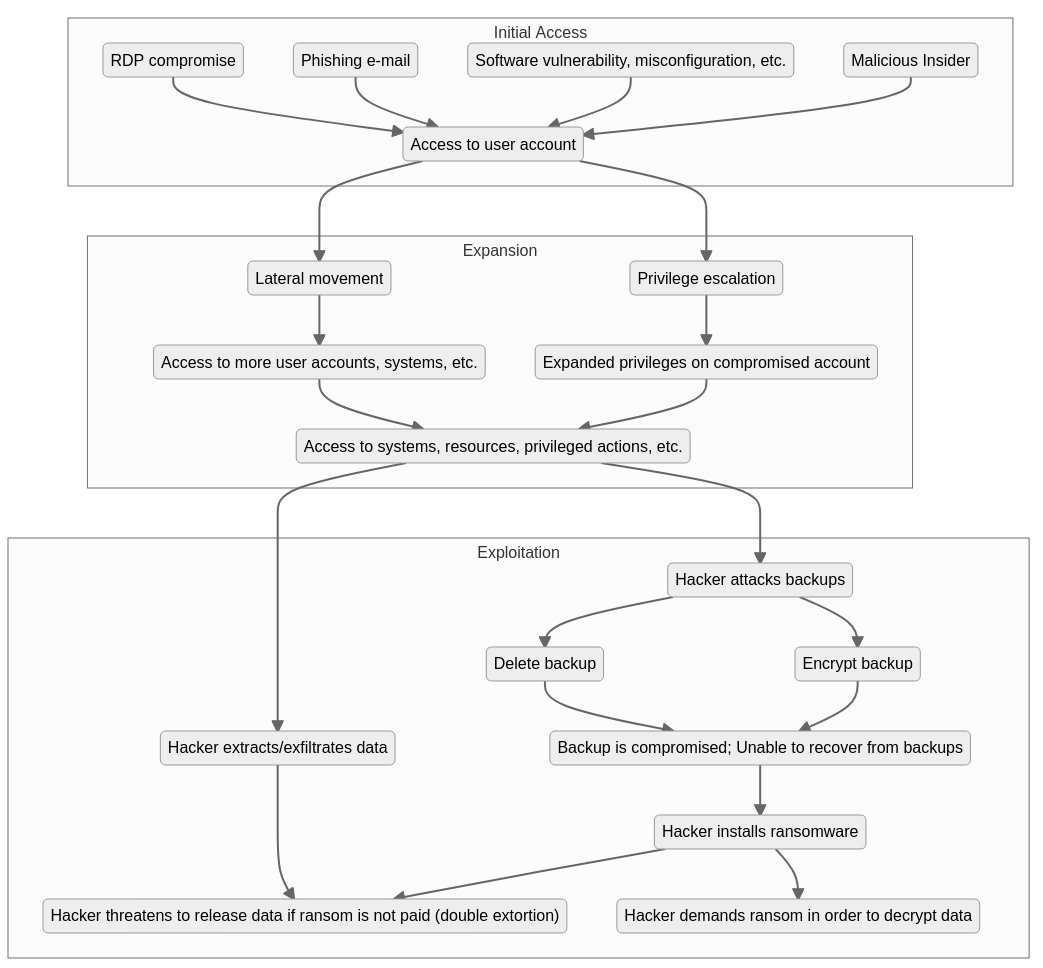
\includegraphics[width=.9\linewidth]{figures/attack_anatomy.png}
    \caption{Illustration of the anatomy of a cyber attack}
    \label{fig:attack_anatomy}
\end{figure}

\subsection{Attacks against backups}
%[TODO] var her 19.mai

Since \gls{backup}s are an essential part of being able to recover from a ransomware attack,
hackers will often try to destroy their victim's backups before encrypting files. Backups are explored in detail in section \ref{Backup}
In this section, we will outline a few possible attack vectors 
against the backups themselves that could try to make them useless.

The simplest way of destroying backups is to simply delete them.
By deleting an organization's backup, hackers can deny recovery, 
which can increase the chance that the organization pays the ransom.

A potential method of corrupting an organization's backups could be to slowly encrypt
the data that is being backed up.
Over time, the backups would be overwritten with invalid data,
making them useless by the time the ransomware is deployed.

A hacker could potentially exfiltrate data from backups.
By encrypting data before backing it up, this risk can be mitigated.
If a hacker exfiltrates encrypted data,
they will not be able to read it without having access to the encryption key used.
    
\section{Backup} \label{Backup}
Faced with ransomware attacks and malicious actors that target the data of organisations, securing that data is essential. It is a fact of living in a digital, interconnected world that malicious actors will attempt to target any data that is available. Face with that risk keeping backups is an important security control.

According to Sjaak Laan, "Managing security is all about managing risks" \cite{laan_it_2017}. Faced with any type of risk, senior management has the option between risk acceptance, avoidance, transfer, and mitigation. While having no data stored digitally, or completely disconnecting all systems from the outside world would be considered avoidance, and some sort of insurance would be considered risk transfer (although almost half of victim organisations that has cyber insurance only got a portion of the losses covered \cite{noauthor_new_nodate}.) An effective backup solution would be an effective risk mitigation technique. 

Laan defines a backup as copies of data, used to restore data to a previous state in case of data loss, data corruption, or a disaster recovery situation. Laan argues that a backup older than a few weeks is of little use, as old, outdated data is probably not very useful for a company in an emergency. The archiving of older data for compliance should be done separately from backups (but should be backed up also) \cite{laan_it_2017}.

Recovery is the process of restoring files from a backup, and is an essential part of any plan to mitigate data loss risk. A backup without a good plan for recovery loses a lot of its use. Recovery should also include procedures for spinning up new VMs as in case of a ransomware attack it would be fair to assume the network to be infected.

In his book "Infrastructure as Code," Kief Morris \cite{morris_infrastructure_2020} argues that in the cloud age organisations should plan for disaster recovery continuously, for example by using the same tools to recover from a disastrous event as an organisation uses to provision and change infrastructure. Recovering from complete disaster should according to him be as easy as anything else. Restoring from a backup in the cloud, and accessing the necessary data on fresh, secure VMs is principal in cloud infrastructure design.

\subsection{Types of backup} \label{Backup Strategies}
There are a few main types of backups that are commonly used.
These are \emph{full}, \emph{differential} and \emph{incremental} backups.
A brief description of each type of backup follows below.

\subsubsection{Full backup}

One of the most straightforward types of backup.
In a full backup, all the data is backed up at once.
Depending on the amount of data, this can take a long time,
and may require a lot of storage.
Recovering from a full backup is usually very simple.
All one needs to do is load the disk containing the backup,
and start the recovery process.

Full backups only require one backup medium 
(unless the amount of data is very large, in which case it needs to be distributed).

\subsubsection{Differential backup}

Differential backups are built upon an existing full backup.
They work by only backing up the changes made since the last full backup, 
instead of backing up all the data.
Since the amount of data changed is generally much lower than the total amount of data,
this is usually faster than doing a full backup every time.

Differential backups require at least two disks, one for the full backup and one for the changes.
Recovery can be done by loading the full backup first, and then the changes.
Recovery from a differential backup is generally slower than from a full backup, but faster than from an incremental backup.

\subsubsection{Incremental backup}

Incremental backups are similar to differential backups,
in that only changes since the last full backup are backed up.
However, unlike differential backups, where all changes since the last full backup are stored,
incremental backups store only changes since the previous \emph{backup activity} (full or incremental).

Recovery from incremental backups consist of first loading the full backup,
then all the incremental backups in order.
This can be a time consuming and complicated process, 
especially if done using physical drives.
Some cloud platforms automate this process,
making it both fast and easy.

\subsection{Database backup}

There are several ways to back up databases.
Many databases support a way to to generate a series of SQL statements that recreate the database.
This is called a \emph{database dump}.
To recover from a dump, the SQL statements are simply run by the database engine.
% This type of backup essentially only stores the data in the database.

Another way to back up a database is to make a backup of the entire virtual machine the database is running on.
This consumes more storage than a dump, but can potentially be faster to recover from,
since software and configuration files are backed up alongside the data.

%-------

\section{The Azure cloud platform}

Microsoft Azure is one of the largest cloud platforms on the market \cite{richter_amazon_2022}.
The platform provides a number of services to organisations that wish to move to the cloud.

% Azure provides a number of relevant security features for creating a secure and effective backup solution. Access to backup data can be protected by role based access control, and multi user authorization, and is only available through Recovery Services vault and Backup vault. 



\subsection{Azure Backup} \label{AZBackup}
Azure Backup is the go-to backup service in Azure. It aims to "provide simple, secure, and cost-effective solutions" for backing up, and recovering data from the Microsoft Azure cloud \cite{v-amallick_what_nodate}.
The service supports a number of services and storage solutions, and the list appears to be expanding.
One month into this project for example, it was announced that Azure Backup now supports the managed Azure Database for PostgreSQL-service that is in the scope of our project, with the release of Azure PostgreSQL backup with long-term retention in February 2022 \cite{noauthor_generally_nodate}. 

Azure Backup offers a number of benefits, according to the Azure documentation \cite{v-amallick_what_nodate}.
The data stored in Azure backup is not directly available to the attacker \cite{terrylanfear_azure_nodate}. 
Protecting backup vaults with Role Based Access Controls (RBAC) is also an important part of protecting the data from ransomware \cite{v-amallick_faq_nodate}. 
RBAC will be discussed in more detail shortly, in section \ref{theory:RBAC}.
%Azure Monitor provides provides ways to monitor actions relating to backups.

Azure Backup has support for backing up a number of different resources. There is support for backing up files, folders, and system state of on-premise systems by using Microsoft Azure Recovery Services (MARS) agent \cite{v-amallick_manage_nodate}.

Backup items are stored in vaults, either a Recovery Services vault, or a Backup vault. Vaults are online storage entities in Azure. According to Microsoft they are designed to make it easier to manage the backed up data. Vaults offer monitoring of the backup data, and configuration of things such as redundancy. Each vault holds data, "such as backup copies, recovery points, and backup policies." \cite{v-amallick_architecture_nodate}

\subsubsection{Recovery Services Vault} \label{theory:rsv}
A Recovery Services vault (RSV) is a type of management entity for backups in Azure.
It is a newer version of Backup vaults with a number of additional features. 
Since its release in 2016, it has been supported with security features like soft delete, Cross Region Restore, and Multi-user authorization \cite{v-amallick_overview_nodate-1}. 
The Multi-user authorization and soft delete features are discussed in sections \ref{MUAtheory} and \ref{Soft Delete} respectively.

Vaults also support a variety of data redundancy tiers (\ref{theory:redundancy-tiers}),
which provide different ways to replicate data across data centers.

The services supported by Recovery Services vaults, according to Microsoft \cite{v-amallick_overview_nodate-1}, are:
\begin{itemize}
    \item Azure Virtual machines
    \item SQL in Azure VMs
    \item Azure Files (Azure Storage)
    \item SAP HANA databases in Azure VMs
    \item Azure Backup server
    \item Azure Backup Agent
    \item DPM
\end{itemize} 

Backup items are held locally, in a storage account, for a while before being transferred to the vault.
Transferring items to a vault can take several hours, but it happens automatically. 
\subsubsection{Backup Vault}
Backup vaults are the older version of recovery services vaults, and therefore offer less functionality.
There is no support for soft delete, Multi-user authorization, or other newer security features.
In 2017 Microsoft announced in a blog post that they would support "seamless upgrade of classic Backup or Site Recovery vaults to ARM based Recovery Services vaults. " \cite{somendra_upgrade_2017}

Backup vaults are still supported in Azure backup to this day,
but its primary use is to be "a storage entity in Azure that houses backup data for certain newer workloads that Azure Backup supports" \cite{noauthor_overview_nodate}.
This includes Azure Database for PostgreSQL servers, and other newer workloads:

\begin{itemize}
    \item Azure Database for PostgreSQL servers
    \item Azure Blobs (Azure Storage)
    \item Azure Disks
    \item Kubernetes Service (Preview)
    \item AVS Virtual machines (preview)
\end{itemize}

\subsubsection{Azure snapshots}
% Building blocks for azure backup

A snapshot typically refers to a read-only point-in-time copy of something,
for example a virtual machine or a hard drive.
Unlike file based backups which store only data files,
snapshots store additional state. %like what

Azure snapshots are read-only copies of a managed virtual hard disk (VHD). % double check managed
These snapshots can be used for backup and recovery purposes.
The snapshots can then be recovered to a new VHD.
If the snapshotted disk was an operating system disk,
it's possible to create a new VM directly from the snapshot.

Azure provides two types of snapshots, full and incremental.
These are essentially implementations of full and incremental backups (see \ref{Backup Strategies}).
A full snapshot makes a copy of the entire disk, 
while an incremental snapshot only makes a copy of the changes since the last snapshot.
Traditionally, incremental snapshots provide faster backup speeds, 
at the cost of a slower and more complex recovery process.
This is not the case with Azure's snapshots.
According to Microsoft blog, 
recovery is almost as fast from incremental snapshots as with full snapshots,
and recovery time is constant no matter how many snapshots are used
\cite{noauthor_incremental_nodate}.
Incremental snapshots in Azure can be deleted without invalidating newer snapshots.

\subsubsection{Azure data redundancy tiers} \label{theory:redundancy-tiers}

Azure provides several tiers of redundancy for data stored in certain Azure services.
These tiers provide different ways of replicating data,
the goal being to prevent data loss in case an incident occurs.
The tiers are described below in order of increasing price \cite{tamram_data_nodate}.

Locally redundant storage (LRS) stores 3 copies of the data, in the same data center.
Zone-redundant storage (ZRS) stores 3 copies of the data, in different data centers in the same region (one copy per data center).
Geo-redundant storage (GRS) replicates LRS from the primary region to a different secondary region ($2 \times 3$ copies).
Geo-zone-redundant storage (GZRS) combines ZRS and LRS. Data in the primary region is stored in ZRS, while data in the secondary region is stored in LRS.

\subsection{Role based access control (RBAC)} \label{theory:RBAC}
In Azure, access to resources is only granted when an identity can be authenticated, 
and it has been assigned the correct permissions. Identites are essentially what seperates different users and resources from each other. Each user has a different identity that is used in RBAC to grant them the access they need. 
According to Modi, in \textit{Azure for Architects}, this is known as authorization, or more commonly as Role-Based Access Control, or RBAC \cite{modi_azure_2019}.
"RBAC in Azure refers to the assigning of permissions to identities within a scope. 
The scope could be a subscription, a resource group, or individual resources."

RBAC helps control which users have access to which resources,
with as much granularity as is needed to segregate permissions within an organisation as well as a single team.
In general it is considered best-practice to only provide the least level of access necessary to perform a task.
Modi argues that separating access between team-members helps ensure both security,
as well as keeping team-members feeling responsible for their jobs as they may be the 
only ones with a necessary level of access to perform some tasks. 
 
RBAC has been an important concept of security administrations since its formalization in 1992, by by David Ferraiolo and Rick Kuhn.
It is the predominant model of advanced access control according to NIST.
One of the advantages of RBAC is that security is managed at a level to closely corresponds to an organization's structure.
Many important security features,
such as multi-user authentication, and the zero-trust model builds upon RBAC.
% , and RBAC is in that way essential for this project.

\subsection{Multi-User Authorization (MUA)} \label{MUAtheory}

While RBAC is useful for administrating access to Azure resources,
it may become useless if an attacker is able to perform a \gls{privilege escalation} attack.
Destructive actions will still trigger alerts for system administrators,
but by the time these are initiated, it may be too late.

Multi-user authorization is a relatively new security feature in Azure which can mitigate this risk.
MUA allows the use of a Resource Guard to protect Recovery Services Vaults in Azure (\ref{theory:rsv}).
This Resource Guard is owned by a different user (the security administrator) in Azure.
The owner of the resource needs to request permission from the security administrator,
in order to to perform destructive actions on the resource \cite{noauthor_protect_2021}.
As a result, no person is solely in control of any task that may be destructive to the backup data.
This can greatly reduce the risk of data loss in case one of the administrator accounts is compromised.

The actions supported by MUA as of this report is:
\begin{itemize}
    \item Disable soft delete
    \item Disable MUA protection	
    \item Modify backup policy	
    \item Modify protection	
    \item Stop protection	
    \item Change MARS security PIN	
\end{itemize}

\subsection{Soft delete} \label{Soft Delete}

Soft delete is a security feature for Azure Backup or Azure Storage Blobs.
When soft delete is enabled, data that is deleted is not removed immediately. 
Instead it is retained for 14 days before being permanently deleted. 
During this time, it is possible to "undelete" the data.
Soft delete is enabled for Recovery Services Vaults by default.

\subsection{Azure Monitor}

Azure Monitor is a service that monitors resources and services in Azure.
If certain actions or events are detected, Azure Monitor can issue alerts to the relevant administrators.
An example is the \textit{Delete Backup Data} alert, which is sent out if any backup data is deleted.
Alerts are either sent to the Azure Monitor view or via email, if it is serious enough.
According to the documentation, certain alerts relating to Azure Backup are sent via email automatically
\cite{v-amallick_monitoring_nodate}.
Custom alert rules can also be configured.


\subsection{Interacting with Azure} 

Azure provides three main methods of interaction:
\begin{itemize}
    \item Azure Portal\\
    The Azure Portal is a graphical interface for managing an Azure environment.
    The Portal is generally quite user friendly.
    \item Azure CLI\\
    The Azure CLI is a set of commands which can be used to manage an Azure Environment.
    The CLI can be accessed through the Azure Cloud Shell, which is a type of console in the Azure Portal.
    The CLI makes it possible to make scripts to automate processes.
    \item Infrastructure as Code (IaC)\\
    Infrastructure as Code is an approach to infrastructure management where resources are
    declared and configured programmatically.
    This can improve stability and reduce maintenance.
    IaC can be implemented using Azure Resource Manager templates,
    or by using third-party tools like Terraform \cite{nishanil_infrastructure_nodate}. 
\end{itemize}

\subsection{Azure Blob Storage} \label{theory:blobs}

Azure Blob Storage is a storage solution in Azure which is optimized for large amounts of data \cite{tamram_introduction_nodate}. 


\section{ClickHouse} \label{Clickhouse}

\subsection{Introduction to ClickHouse}
% [TODO] Fylle ut

ClickHouse is a database used for Online Analytical Processing (OLAP).
It is highly optimized for certain types of workloads,
and is able to process large amounts of data in an efficient manner \cite{noauthor_what_nodate-2}.

ClickHouse runs as a server on a virtual machine,
which can be accessed using the program \texttt{clickhouse-client}.
ClickHouse uses SQL as its query language.

\subsection{Backup solutions for ClickHouse} \label{theory:ch-solutions}

According to the ClickHouse Documentation, there is no universal backup solution for ClickHouse,
but the documentation contains a few different suggested solutions \cite{noauthor_data_nodate}.
In this section, we will provide a short summary of the solutions listed in the documentation.

\begin{itemize}
    \item Duplicating Source Data Somewhere Else \\
    A program such as Apache Kafka can be used to serve a stream of data as input to ClickHouse.
    This stream can be forked and diverted to send data to backup storage at the same time as it is sent to ClickHouse.
    \item Filesystem Snapshots \\
    Some filesystems like ZFS support making \emph{snapshots} of the filesystem's state.
    These snapshots can then be sent to an external storage solution.
    \item clickhouse-copier \\
    clickhouse-copier is a tool that can be used to copy data between ClickHouse clusters.
    Originally intended for petabyte-sized databases.
    \item Manipulations with Parts \\
    A local copy of a table can be made with ClickHouse's built-in \texttt{ALTER TABLE FREEZE} query.
    The copy can be exported with a program like \texttt{rsync}.
    \item clickhouse-backup  \label{theory:chbk} \\
    clickhouse-backup is a tool that automates the \emph{manipulations with parts} approach.
    The tool is installed on the same server as ClickHouse.
    It can store backups locally or on a remote server, using various storage methods,
    like Azure Blob Storage or AWS S3 object storage.
\end{itemize}

\subsection{Backup solutions for ClickHouse in Azure}

Azure provides tools for backing up data.
These are not mentioned in the ClickHouse documentation,
since they are not specific to ClickHouse.
Azure Backup supports backing up individual virtual machines as described in \ref{AZBackup}.
This feature can be used to back up the VM running ClickHouse.

%-----------

\section{PostgreSQL} \label{Postgres}

\subsection{Introduction to PostgreSQL}
PostgreSQL is an open-source relational database management system (RDBMS). It is suited for operations requiring complex SQL queries, and provides functionality enabling data analysis. Azure has its own hosted solution called Azure Database for PostgreSQL, which automates maintenance, patching, and updates \cite{noauthor_azure_nodate}. It also allows effortlessly scaling the database size and computing.

 There are only a few backup options that are relevant to look into when working with a managed PostgreSQL instance hosted in Azure. This short introduction will also include frequently seen practices for unmanaged instances of PostgreSQL before narrowing the focus into managed ones hosted on Azure.

% TODO: Say something about the managed Postgres service in Azure

\subsection{Backup solutions for PostgreSQL}

One recovery option for protecting backup could be removable storage.
This will however not be the focus when exploring options for a ransomware-resistant backup architecture.
 
Some options for backing up a PostgreSQL database include extraction of data using the pg{\_}dump command. This way one could back up data off-site for increased security by air-gapping, although setting this up in such a way that RTO and RPO are met can prove challenging. Moreover, a backup restore from a remote server takes longer time than a local copy. 

\subsection{Backup solutions for PostgreSQL in Azure}

%-----------
\subsubsection{Azure Backup} \label{theory:PITR}
Azure Database for PostgreSQL backup has long-term retention in Backup Vaults. A backup vault is a storage entity housing backup data in Azure \cite{v-amallick_overview_nodate}. It requires connecting to a Key Vault to integrate with the database instance that will be backed up. Azure Key Vault stores and allows accessing secrets \cite{noauthor_key_nodate}. Examples of secrets could be API keys, passwords, certificates, or cryptographic keys. In this case, it is the database connection string.

The Backup Vault has long-term retention of up to 10 years. It also allows configuration and granular control allowing for a backup policy that complies with the organisations needs.

%A distinction here has to be made between Azure Database for PostgreSQL backup and the native backup solution offered by Azure PostgreSQL. The main difference between the two is the period of time that data is retained and the customization options. Azure Database for PostgreSQL backup has long-term retention of up to 10 years. It also allows configuration and granular control allowing for a backup policy that complies with the organisations needs.
%En del av dette under må omskrives med egne ord, noe er tatt ordrett fra dokumentasjonen.
%In addition to this there are multiple features such as scheduled and on-demand backups at database level. It is also possible to create a backup of the PostgreSQL server database to another server or to Azure blob storage. 
%Compartmentalisation and isolation to a certain extent also follow with Azure Database for PostgreSQL where backups are stored in separate security and fault domains. 
% Explain security and fault domains here.
%Lastly, use of pg\_dump can allows for restoration across database versions.

\subsubsection{Point-in-time-Restore} \label{theory:PITR}
In contrast, the built-in Point-in-time-Restore (PITR) solution has a default retention of only 7 days, which can be set to a maximum of 35 days. If the server size is up to 4TB the native solution operates on two differential backups a day and a full backup once a week. If larger than 4TB and up to 16TB, the solution operates on snapshot based differential backup, with three snapshots performed in a day.
% Her må det omskrives litt der det ligner for mye på docs fra lenken under.
% https://docs.microsoft.com/en-us/azure/backup/backup-azure-database-postgresql-overview

The built-in backup solution and the Azure Database for PostgreSQL backup can operate simultaneously. 

\section{Security Best Practices} \label{BestStrat}

\subsection{Principle of least privilege}
When assigning permissions to users and processes to access resources in an organisation, it is considered best practice according to the principle of least privilege to only give the minimum level of access needed at any given time. For example doing menial tasks like checking emails and browsing the internet should not be done while accessing a system as administrator. In modern systems architecture the role of system administrator should not be used instead, access should be provided only to the resources a user needs at at given time \cite{ramel_anatomy_nodate}.
In Azure, this is implemented with RBAC (\ref{theory:RBAC}).

\subsection{Zero trust}
One of the modern mainstays of cybersecurity and infrastructure security is the Zero Trust model.
The National institute of standards (NIST) special publication 800-207 provides the following definition: 
"Zero trust provides a collection of concepts and ideas designed to minimize uncertainty in enforcing accurate,
least privilege per-request access decisions in information systems and services in the face of a network viewed as compromised." 
\cite{cybersecurity_and_infrastructure_security_agency_cisa_2021} 

This definition says that one should view the network as compromised,
and as such bear that in mind for every decision made when designing the network.
The alternative, assuming a network or system is not compromised,
has disastrous consequences if this assumption is incorrect.
This can be exemplified by Ramel's retelling of a ransomware attack where the cause of the breach was an administrator logging in to a compromised system to perform mundane tasks with admin privileges \cite{ramel_anatomy_nodate}. The attacker would not have been able to gain admin rights if it hadn't been for the unnecessary use of the administrator account. \label{ZeroTrust}

Zero Trust architecture is described by CISA as fundamentally different from prior models,
and one that will require a holistic change in the way an organisation thinks about its cybersecurity controls,
but also its philosophy and culture around cybersecurity. 

The core concept of a Zero Trust architecture is that security is no longer perimeter-based,
and that there is an implicit assumed threat in any network.
Therefore the security model focuses on data and service protection,
and only providing the minimal level of access to resources and data when, and only when, that access is needed.
Trust and access must always be continually evaluated,
and an attacker won't have free reign of all resources once inside a network.
The model aims to hinder the unauthorized lateral movement of attackers inside networks once the perimeter is breached 
\cite{rose_zero_2020}. 

The same source describes a number of factors that may enable a system to grant or deny access to a resource. A trust algorithm uses these factors to make a decision on whether or not it is likely that the request is legitimate, and denies it if it is not likely. The trust algorithm can be run multiple times during a session to continually confirm the legitimacy of the access given to a subject. 
 
% \subsection{Automation solutions} \label{IaC}
% Infrastructure as Code is a broad subject, and far beyond the general scope of this project, however some key aspects should be mentioned. Morris' book on the subject is already mentioned in this report, and it supports the claims in this subsection. 
% 
% Whilst designing infrastructure solutions in the cloud system architects should attempt to leverage any and all benefits of a cloud environment if they can. One of these benefits that Morris mentions early and often is to assume systems are unreliable. In essence, an organisation can't expect a VM to remain stable and running into eternity. This, he argues, means that systems should never be modified after creation. 
% 
% It ties into another key principle of his, which is to make everything reproducible. That means that any infrastructure in a system should be able to be rebuilt completely and still function as intended and according to the needs of the organisation. 
% 
% The argument for automation is supported by security architect in CheckPoint, Pål Aaserudseter, who says in an interview with digi.no that by 2025, 99\% of security incidents will be caused by human error. \cite{samsonsen_sikkerhetsarkitekt_2022} Norkarts data leak that was reported on the 10th of may 2022, is an example of this, as the cause of the breach was a misconfigured firewall. \cite{samsonsen_persondata_2022} 

%-----------

\chapter{Method}

\label{Method}
\section{Chapter outline}
To answer the research questions presented in section \ref{RQ}, we conducted a number of experiments on two different databases with two different backup solutions in place for each of them. 
The goal was to use our findings in the experiments to get a good overview of security features in Azure,
in order to be able to answer our research questions.
The basis for our experiments was three scenarios that represent different attack vectors that the databases must be secured against. 

In the discussion chapter (\ref{Discussion}), we compare and contrast the different backup solutions used in the experiments. This is so that we can determine which security features are worth implementing, how secure they are, and how they impact the overall backup architecture. This is also used to help answer the research questions. More general requirements for backup solutions, such as performance and cost, were also considered.
Because of this, a performance test was performed for each backup solution in order to aid in the comparison. 

In this chapter we present the method for our analysis, and describe in detail how we worked to find the results presented in chapter \ref{Results}. We start off with describing the criteria used in our analysis in section \ref{criteria}. In section \ref{BackupSolutions}, we present the two databases we implemented backup solutions for, and their backup solutions. We then describe how they were deployed in section \ref{Deployments}. 

The scenarios are at the center of our analysis.
Their results are based on the criteria in \ref{criteria}, and are performed in the test environments described.
The scenarios are described in section \ref{Scenarios}, where we also describe the experiments that will be
For each of the three scenarios, several experiments were performed.
for each of them and how these were performed is described in detail.
Finally, in section \ref{Perftest} we describe how the performance of the backup solutions were tested.

\section{Criteria for analysis}
The backup solutions we describe in \ref{BackupSolutions} were evaluated based on the criteria we describe in this section. These are important criteria to assess the security of the different backup solutions. 
\label{criteria}
\subsection{Resistance to ransomware attacks}
Since the topic of our thesis was to analyse cloud backup architectures with regards to their resistance to ransomware attacks, resistance to ransomware is the most important criteria to evaluate backup solutions by. Though this is a measure that can be hard to quantify, several factors are taken into consideration when evaluating the 
ransomware resistance of a backup solution.

% Having an idea of the cyber risk quantification, i.e., what damages the company might suffer given a ransomware attack, certainly helps deciding resistance measures which mirror the cyber threat landscape. 

Specific properties to keep in mind when evaluating the ransomware resistance of a system are:
\begin{itemize}
    \item Ability to recover encrypted files.
    \item Ransomware detection. % maybe out of scope
    \item Ability for backup to withstand encryption.
    \item Ability for backup to withstand deletion.
\end{itemize}

Each backup solution's resistance to ransomware was assessed qualitatively.

\subsection{Ease of use}

There is often a trade-off between security and ease of use. Disconnecting a database server from all networks would essentially render it immune to ransomware attacks over the network, but it would also be incredibly inconvenient. An acceptable backup solution needs to be secure enough to be able to  resist ransomware attacks, while at the same time being easy to set up, automate and maintain. Humans are fallible, and if the backup solution is too troublesome to use, the maintainers might neglect to verify that everything is working correctly.
If security measures interrupt the operations of those using the services that are being protected, the users might seek out ways to bypass them.

Each backup solution's ease of use was assessed qualitatively throughout the experiments, based on our experience using them. We focused on the ease of setup, ease of maintenance (regular testing), and ease of recovery in the event of an attack.

\subsection{RPO and RTO} \label{method:rtorpo}

Recovery Point Objective (see \ref{theory:rpo}) and Recovery Time Objective (see \ref{theory:rto}) are two essential parameters to keep in mind when evaluating backup architectures. 
It is up to each organization to determine their own required RPO and RTO,
based on cost-benefit analyses and other considerations.

RPO was analyzed by looking at the options provided by each backup solution with regards to options for specifying the frequency of creating recovery points. RTO was analyzed by conducting performance tests (see \ref{method:perf}).

\subsection{Cost}

More secure solutions are generally more expensive. Cloud platforms charge for the amount of data stored in their services, and that includes backups. While we can't decide if a backup solution is too expensive or not, we considered the cost of the different solutions in our general comparison. 

\section{Backup solutions to analyze} \label{BackupSolutions}

In our analysis we considered each scenario, and created experiments for backup solutions for two different databases. The two databases were an unmanaged ClickHouse database running on an Azure VM, and an Azure Database for PostgreSQL instance, which is a managed database in Azure. This means that each scenario is analyzed twice; once for each of the two databases. The databases are detailed in sections \ref{Clickhouse}, and \ref{Postgres} respectively.

\subsection{Backup solutions for ClickHouse}

Our experiments focused on two backup solutions for ClickHouse. 
These were Azure Backup for VMs, a service provided by Azure, and clickhouse-backup, a third-party tool for backing up ClickHouse databases specifically.
%Backing up the entire VM with the running database and its data with Azure Backup, and clickhouse-backup, a third-party backup solution for Clickhouse databases. 

\subsubsection{Azure Backup} 

Azure Backup (see \ref{AZBackup}) was chosen as one of the backup solutions to test for ClickHouse. It provides tools for easily configuring automatic backup for Azure VMs. Since it backs up entire VMs, and not just the specific database's data, it can essentially be used to back up any service running in a VM.

Since Azure Backup stores backed up VMs in Recovery Services vaults (see \ref{theory:rsv}), all the security features of these newer vaults are available for this backup solution.

\subsubsection{clickhouse-backup}

Of all the backup solutions listed in the ClickHouse documentation (see \ref{theory:ch-solutions}), clickhouse-backup seemed like the most appropriate one. clickhouse-backup can back up data locally and remotely, and supports integration with different cloud providers. 
One of the supported remote storage solutions is Azure Blob Storage (see \ref{theory:blobs}), which is a cheap storage option.

\textit{Duplicating Source Data Somewhere Else} was ruled out because it requires the use of a persistent queue, which is not relevant to our case. \textit{Filesystem snapshots} were ruled out because we are not using a filesystem with snapshot functionality. \textit{clickhouse-copier} was ruled out because it is designed for petabyte-sized databases \cite{noauthor_data_nodate}, which seems overkill for our use case.

\subsection{Backup solutions for Azure Database for PostgreSQL}
For PostgreSQL we also tested two different backup solutions. Azure Backup for PostgreSQL, and the Point-in-time-restore (PITR) functionality of the Azure database for PostgreSQL service. These services were able to be used separately or together as part of a holistic solution.

% The perceived ease-of-use and security features of the solutions are what led us to choose them over other, more complex, but likely not as secure, such as pgdump.

\subsubsection{Azure Backup for PostgreSQL}
Azure Backup started supporting PostgreSQL in January 2022. Because it is still relatively new it is not supported by Recovery Services vaults. Instead, it uses the older Backup Vaults in Azure. This means that far fewer security features are supported compared to the Azure Backup solution for VMs. Even so, this solution supports 10 years of data retention, scheduled and on-demand backups and backup restoration, either directly to a database or as a file in Azure Blob Storage. 

\subsubsection{Point-in-time Restore}
Point-in-time Restore is a feature of Azure Database for PostgreSQL that allows restoring the database to any point within the last 35 days, depending on settings. It is described in more detail in \ref{theory:PITR}. This provides a lot of flexibility when it comes to choosing which restore point to restore to. 

\section{Test environments} \label{Deployments}

In this section, we describe how the test environments were deployed and configured in detail. 
% The databases and backup solutions are the ones described in section \ref{BackupSolutions}

\subsection{Illustration of test environment}
The test environment is illustrated in Figure 3.1, and shows the databases we used in our analysis, as well as their backup solutions. The red bordered area shows where the backups are stored within the architecture. Each scenario will attack some part of this architecture, and the experiments will show how to recover the lost data, or otherwise mitigate the risk associated with the attack. 

\begin{figure}[h!]
    \centering
    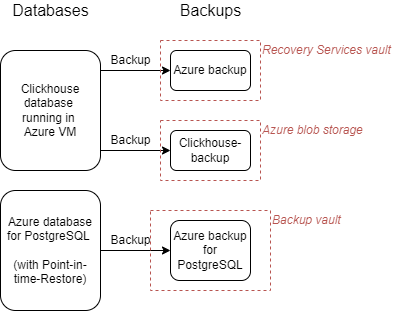
\includegraphics[width=.9\linewidth]{figures/Backupsolution.png}
    \caption{Illustration of the databases and their backup solutions}
    \label{fig:backup_architecture}
\end{figure}

\subsection{Test environments for ClickHouse}
%as well as our rationale for choosing which solutions to test.
\subsubsection{Test environment for non-performance sensitive tests} \label{method:ch-non-perf}
In order to perform experiments where performance was not being measured,
we set up a simple test environment.
The test environment consisted of a single Linux VM running Ubuntu 16.04.
The VM size selected was "Standard B1s" \cite{rishabv90_b-series_nodate}, which is a general purpose VM with
a single vCPU, 1GB of RAM, and a 30GB SSD. 
ClickHouse and clickhouse-backup was installed on the VM and configured. In addition, Azure Backup was set up. A data set of around 700MB (when compressed by ClickHouse) was used. A detailed overview of how the non-performance critical test environment was set up is included in the appendix, see \ref{app:ch-non-perf}.

\subsubsection{Test environment for performance tests}

For performance tests,
a different test environment was used.
A more powerful VM was necessary in order to 
avoid bottlenecks that could interfere with the performance test results.
The VM size selected was "Standard D4s v4" \cite{andysports8_dv4_nodate}.
This is a general purpose VM with 4 vCPUs and 16GB of RAM.
16GB of RAM is less than the amount recommended for ClickHouse \cite{noauthor_usage_nodate} but greater than the minimum requirement \cite{noauthor_requirements_nodate}.
The reason we chose this VM size was because it was the largest size available with our Azure subscriptions vCPU quota.
This is unfortunate, but we believe it was sufficient for our tests.

The OS disk size selected was 2048GB, which was enough to leave some overhead after loading the test data. The uncompressed size on disk of the data set used was around 5TB. The data set was compressed to a size of 955GB by ClickHouse. We believe this amount of data should be enough to give a realistic overview of the performance of each backup solution.

For a detailed overview of how the performance test environment was set up, 
see \ref{app:ch-perf} in the appendix.

\subsection{Test environment for PostgreSQL}
We tested Azure database for PostgreSQL with the \texttt{GP\_Gen5\_2}-SKU, a general purpose configuration that is similar to the needs of most businesses. The setup was done with a PowerShell script for repeatability, and can be seen in appendix \ref{pg_setup}. Point-in-time-restore is enabled by default (and can not be disabled.) 

Connecting to the PostgreSQL instance was done with pgAdmin 4.
This is a tool used to manage PostgreSQL databases.
Another option here would have been using Azure Data Studio.
% which would require installing the PostgreSQL extension. 

We populated the database with data using a script.
See appendix \ref{pg_populate} for details.
%in order to show data loss and restoration in the experiments. 

In order to protect PostgreSQL with Azure Backup, we created a Backup vault and deployed a backup instance with an accompanying backup policy for the PostgreSQL server within it. 
The process is described in detail in appendix \ref{pg_azurebackup}. 

\section{Scenarios} \label{Scenarios}
In order to evaluate the effectiveness of each of the backup solutions, we came up with three practical scenarios. These are imagined attacks against the databases or backups, which the backup architecture has to be able to withstand.

These scenarios were used as a basis to create experiments, which are practical demonstrations of how an attack could be carried out, and how the system would recover from the attack, or otherwise how the risk of the attack may be mitigated. The scenarios are also used to provide a meaningful context for discussing each backup solution's resistance to ransomware. 

\subsection{Scenario 1: Attacker encrypts database data}

This first scenario is perhaps the most central scenario for the project.
This is essentially a basic ransomware attack, where only the data stored on the database servers are encrypted.
This attack is illustrated in figure \ref{fig:scenario 1}.

\begin{figure}[h!]
    \centering
    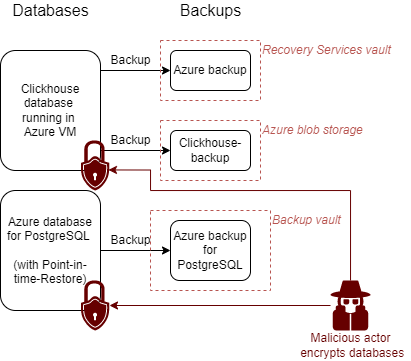
\includegraphics[width=.9\linewidth]{figures/Scenario1.png}
    \caption{Illustration of Scenario 1, a malicious attacker encrypting databases}
    \label{fig:scenario 1}
\end{figure}


\subsubsection{Conditions}
This scenario assumed an attacker has managed to gain access to the database-server, or the server that configures it. The attacker has also managed to elevate their privileges enough to delete or encrypt data. The attacker is not necessarily sophisticated enough to look further into the system,
or attempt to counteract the security controls in place. 

\subsubsection{Consequences}
The worst case consequences of this scenario is complete data loss.
Given that the attackers are using a modern strain of 
ransomware with sophisticated encryption schemes,
as it is fair to assume, the encrypted data could be completely lost.
This attack without a plan for data restoration could force the 
victim organisation to pay the ransom or risk bankruptcy 
especially if the data is business-critical. 

\subsubsection{Risk Mitigation}
Recovering from this attack involves restoring the data in the databases from backup. As the goal of the attack is to ensure the organisation loses access to their data, and making the ransom the only viable method of recovery, our goal should be to ensure another method of recovery exists. 

In our case, recovery from this scenario involved verifying that the backup solutions reliably backed up data, and that the data restored from them was the same as we backed up. 

\subsubsection{Testing}
To test this scenario we encrypted or deleted data in each database. Each of these has backups that we then restored from. In addition to testing that restoring from these backups works, we noted significant aspects of the recovery process in order to better evaluate the non-functional attributes of the backups. 

\paragraph{ClickHouse experiment:} 

To test this scenario with ClickHouse, we ran an experiment where we encrypted certain files in \texttt{/var/lib/clickhouse/}. This is the default storage path for ClickHouse. The files were encrypted using an encryption tool called \texttt{ccrypt}. The full details of how this experiment was conducted can be found in section \ref{app:chs1e1} of the appendix.

A short summary follows here.\\

\noindent
The files we encrypted were files that correspond to columns in a database table.
We tried encrypting both a single file and the whole directory containing the files.
The effects the encryption had on the database were observed.
Then, the database was recovered using backups from clickhouse-backup and Azure Backup.

The following files were encrypted:

\begin{itemize}
    \item \path{/var/lib/clickhouse/store/c28/c283470d-9ab3-4be8-bd81-132274c9f9b0/all_1_35_2/radio.bin}
    \item \path{/var/lib/clickhouse/store/}
\end{itemize}

\paragraph{PostgreSQL experiments:} % [TODO] Åsmund eller Omer les gjennom og godkjenn endringer
We find it unlikely that a normal ransomware virus would be able 
to encrypt data in a managed PostgreSQL database. It is however not unlikely that future threat actors target managed cloud services to a greater degree than is normal now, as more organisations move to the cloud
To test this scenario we will, instead of encrypting tables, 
simulate an attack where the tables in the database are dropped.
This gives us an opportunity to test how recovery is performed with each backup solution.


The first backup method that was tested was Point-in-time restore (PITR).
The table was dropped and then restored with PITR.
The experiment is described in detail in the appendix (\ref{app_pg_s1e1}). 
%In this experiment we used the built-in PITR feature,
%and restored to a new database server instance in order to restore the data in a safe environment. 

To test recovery with Azure Backup for PostgreSQL,
we once again dropped the table and started recovery.
The Backup vault GUI for Azure Backup for PostgreSQL was used to restore to a new database from the latest backup available.
This is described in detail in appendix \ref{app_pg_s1e2}.

\subsection{Scenario 2: Attacker deletes backups}
In a human-operated ransomware attack, it is likely that the attacker would attempt
to delete backups before deploying the ransomware itself. Figure \ref{fig:scenario 2} shows the attacker deleting the backups in our test environment. 
\begin{figure}[h!]
    \centering
    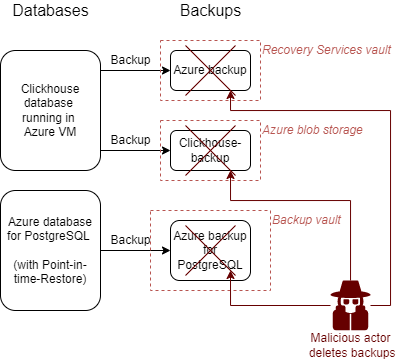
\includegraphics[width=.9\linewidth]{figures/Scenario2.png}
    \caption{Illustration of Scenario 2, a malicious attacker deleting backups}
    \label{fig:scenario 2}
\end{figure}

\subsubsection{Conditions}
The attacker would need access rights at a high enough level to threaten the backups. Whereas in scenario 1 the attacker only needed access to the specific data they attempted to ransom, the attacker would in this scenario also require access to the backup administrator's Azure account, or an account with equivalent privileges over the backups.   

\subsubsection{Consequences}
This attack is unlikely to be devastating on its own, 
but if the attacker is able to delete or encrypt the data in the databases as well, 
this could be crippling for an organisation. 
The ultimate consequence of such an attack would be total data loss.

\subsubsection{Risk Mitigation}
Preventing this scenario from even occurring is critical to any backup implementation. If for example a compromised administrator has access to both the database and the backup, they become a single point of failure for the whole system. 

A number of attacks may be avoided if there are routines to monitor logs and alerts that may tell the organisation that something is wrong. Even if an attacker is able to bypass the security features protecting the backups, there ought to still be someone monitoring any log entries or alerts that this is happening. This would let the organisation preemptively try to mitigate the attack, and ideally lock the attackers out of the network.

Even if the backups are deleted, they may still be recoverable. By default Recovery service vaults has soft delete (see \ref{Soft Delete}) enabled, which would allow the organisation to recover their backups, and then recover their data from them. Note that Backup vaults do not supports soft delete. Soft delete can also be enabled for Azure Storage Blobs.

\subsubsection{Testing} 
In order to test this scenario, we attempted to delete backups made with the different backup solutions.
After this we attempted to restore them and recover data from the now undeleted backups.
Where that was not possible we also looked into other security mitigation possibilities.

\paragraph{ClickHouse experiments:} 

For ClickHouse, four experiments were performed.
These all involved destroying backups in different ways.

In the first experiment, local backups made with clickhouse-backup were encrypted using the tool \texttt{ccrypt}, and the results were observed. We attempted to list and restore the encrypted backup using \texttt{clickhouse backup list} and \texttt{clickhouse backup restore} respectively. See the appendix (\ref{app:chs2e1}) for full details regarding how the experiment was carried out.

Clickhouse-backup has commands for deleting local and remote backups 
(\texttt{clickhouse-backup delete [local/remote]}).
In the second experiment, backups made using clickhouse-backup were deleted using these commands.
This was done in order to simulate an attack where the attacker has root access to the VM,
but not to the Azure environment itself.
Afterwards, the deleted backups were recovered by
undeleting the Blobs via the Azure CLI,
and then restoring the database with \texttt{clickhouse-backup restore\_remote}.
See the appendix (\ref{app:chs2e2}) for the full details.

The third experiment was similar to the second, 
in that remote backups made using clickhouse-backup were deleted.
This time, they were deleted  using the Azure CLI,
in order to simulate an attack where  the attack has access to an Azure Cloud Shell session.
Afterwards, the backups were once again recovered by undeleting
the Blobs using the Azure CLI and then restoring the database with \texttt{clickhouse-backup restore\_remote}.
See the appendix (\ref{app:chs2e3}) for the full details.

In the fourth experiment, backups made using Azure Backup were
deleted, and then restored from their soft deleted state.
Both deletion and restoration was performed using the Azure CLI.
See the appendix (\ref{app:chs2e4}) for the full details.


\paragraph{PostgreSQL experiments}
Backups for a managed PostgreSQL database are inherently tied to the database, due to its point-in-time restore (PITR) function. To test this scenario, we therefore deleted the database server instance in an attempt to delete the backup, and then restored it from PITR. When creating a new managed PostgreSQL Azure Database the option is given to restore from a PITR-point. This allows the database to be "undeleted" in practice, as long as it is restored within the restore period. This process is shown in \ref{app_pg_s2e1}.

As Backup vaults, which Azure Backup for PostgreSQL uses, does not support soft delete functionality, the experiment for the Azure Backup solution was simply to delete the backup instance in the Backup vault. %The process is described in detail in appendix \ref{app_pg_s2e3}.
After doing so, there was no option to undelete or restore the backup data. 

In addition to restoring the deleted backups, one important risk mitigation effort would be to ensure that the backup administrator is alerted when backup data is deleted. 
Azure Database for PostgreSQL does not automatically alert the backup administrator when backup data is deleted.
Alerts will also have to be monitored elsewhere than the Backup Center, as no alerts have shown up here throughout our testing.

We created an Alert Rule that sent an alert each time the "Microsoft.DataPro-tection/backupVaults/backupInstances/delete" action succeeded within the scope of the subscription containing the Backup vault. This is the action which deletes backup instances in backup vaults. This rule was linked to an Action Group that sent an email to the backup administrator each time the Alert was delivered. This could also be sent as a phone notification or a text message. This alert rule is described in detail in appendix \ref{app_pg_s2e2}. 

\subsection{Scenario 3: Backup administrator compromised}
The third scenario assumes a complete compromise of the backup administrator account.
This account has administrator access to the vaults in Azure,
or has other permissions allowing them to modify or delete backups, or change security settings.
In the previous scenario we looked at how to mitigate risks associated with a lost or deleted backup. This time the attacker has access to the backup administrator account and can disable whatever security settings or delete whichever resources they wish. 

This attack is illustrated in figure \ref{fig:scenario 3}, which shows the backup administrator account controlled by the malicious actor, as well as the domain which the backup admin account controls.

\begin{figure}[h!]
    \centering
    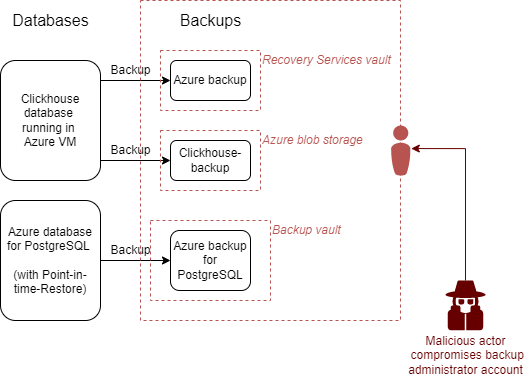
\includegraphics[width=.9\linewidth]{figures/Scenario3.png}
    \caption{Illustration of Scenario 3, a malicious attacker compromising backup admin}
    \label{fig:scenario 3}
\end{figure}

\subsubsection{Conditions}

The condition for this scenario to occur is simply that an attacker has gained access to the backup administrator account. As discussed in section \ref{ZeroTrust}, this can easily happen through simple human error, or misuse of administrator accounts when performing mundane tasks.

\subsubsection{Consequences}
One of the consequences of this scenario is the permanent loss of all data, given that the attacker is able to disable soft delete and delete all backups and deploy ransomware shortly thereafter. Ransomware operators spend weeks trying to figure out all there is to know about an organization, and if they see an opportunity to attack both the databases and their backups simultaneously, they are sure to grab it. 

\subsubsection{Risk mitigation}
There are security features in Azure to prevent a compromised administrator account from disabling soft-delete and deleting backups. One of them is Multi-user authorization, as described in \ref{MUAtheory}. In addition to that feature in particular, well designed access control in general, based on Role-based access control, and Zero-trust features such as Just-in-time access can prevent this scenario from resulting in any major consequences.
 
\subsubsection{Testing}
Testing for this scenario involved exploring how much data could be made irrecoverable with full access to the backup resources in Azure, 

\paragraph{ClickHouse experiments:}

We performed 3 experiments for this scenario in Clickhouse.

In the first experiment, 
soft delete was disabled for a protected item in Azure Backup before the item was deleted using the Azure CLI.
See the appendix (\ref{app:chs3e1}) for the full details.

In the second experiment, the entire Recovery Services vault used to store Azure Backup backups
was deleted using a PowerShell script.
See the appendix (\ref{app:chs3e2}) for the full details.

In the third experiment, we once again attempted to run the Recovery Services vault deletion script,
but before doing so, we enabled Multi-user authorization and observed what happened.
See the appendix (\ref{app:chs3e3}) for the full details.

\paragraph{PostgreSQL experiments:} \label{pg_sc3}
Since there it is not possible to disable the soft delete feature of PITR, this scenario is less relevant for PostgreSQL compared to ClickHouse. Backup vaults support neither soft delete nor MUA, so this scenario does not have a direct solution using Azure Backup either.  

\section{Performance testing} \label{Perftest}

In order to determine whether it is realistic that a backup solution 
is able to recover data within a given RTO,
we conducted performance tests for each backup solution.
The performance tests measure how long it takes to restore a database of a certain size.
This is a useful parameter to consider when comparing the different backup solutions.  

\subsection{Performance tests for ClickHouse}
ClickHouse is able to handle large amounts of data,
which means a backup solution for ClickHouse should also be able to.
We decided to load ClickHouse with 1TB (compressed) of data,
which we believe was enough to get a realistic idea of
the backup solutions' performance.

For the Azure Backup test, we first prepared the environment by deleting the VM, listing the available restore points, and then selecting which restore point to use. A stopwatch was started the moment we initiated the restore job. The stopwatch was stopped when it was possible to connect to the VM using SSH and run database queries. The time used by the restore job itself is printed of the command 
\noindent \texttt{Restore-AzRecoveryServicesBackupItem}.
This was noted separately.
See \ref{app:chab-perf} in the appendix for the full details regarding how the tests were performed.

For clickhouse-backup, the plan was to measure the time it took to create a new VM with the necessary software,
using a stopwatch.
Then, the builtin command \texttt{time} was to be used to measure the time used by the
\texttt{clickhouse-backup restore\_remote}.
Afterwards, the times were to be summed up to get the total restore time.
However, we experienced errors we were not able to resolve, which prevented us from carrying out the test.
Appendix \ref{app:chbk-perf} contains details about how the tests were performed,
and what went wrong.
This is also discussed in chapter \ref{Results}.

%, we first measured the time it took to create a new VM and install the necessary software with a stopwatch. Then we used the builtin shell command \texttt{time} was used to measure the time used by the command  \texttt{clickhouse-backup restore\_remote}. The times were then summed up. See \ref{app:chbk-perf} in the appendix for the full details regarding how the tests were performed.

\subsection{Performance tests for PostgreSQL}

The following experiments compared the performance of Azure Database for PostgreSQL single server when restoring using different methods. A general purpose single server with 4 vCores and 100 GB of storage was deployed in the same way as for our other testing, as seen in \ref{pg_setup}.

We populated the databases with data using a script (see appendix \ref{pg_populate}). 
The script generated 7107MB of data.

% Connecting to the database using pgadmin4 and running the psql command below returned a size of 7107 MB.
% 
% \begin{minted}[breaklines=true,breakanywhere=true]{sql}
% SELECT pg_size_pretty( pg_database_size('postgres') );
% \end{minted} 


\subsubsection{Delete server and restore using backup vault}

After deleting the data in the database we recorded how long it took to restore the data to a running PostgreSQL-instance. 

%If archive then could take longer,.. Backup vault test was performed a newly full backup, while PITR uses transactional history as well as differential backups to build back to a previous state.

HER TRENGS DET Å SKRIVES MER/TYDELIGERE.

This was sufficient for a baseline test. Further, a key vault was deployed which the backup vault linked to for access to the connection string necessary to work with the PostgreSQL single server. 

The goal was measuring the restore time after deleting a server. 

\subsubsection{Delete server and restore using point-in-time restore}

A test similar to the previous was performed with point-in-time Restore.
PITR has an option to create a new server from the restore point,
which is what was used in this test.

% Azure has the option of point-in-time restore to a new server which is tested out with the same database and single server configuration as the one used in the backup vault performance test above. The difference in implementation was that PITR creates a new server as part of the restore process, while the same has to be done as a separate operation for backup vault.

\chapter{Results}
\label{Results}
In this chapter, we present the results of the analysis described in chapter 3. We present these results separately for ClickHouse and PostgreSQL in order to more easily look at them holistically here and in the discussion later. 

As this project analyzes the different backup solutions qualitatively, the results are based on our evaluation of how well each experiment highlights the resistance to ransomware of each backup solution, as well as their ease of use.   

\section{ClickHouse}

\subsection{Scenario 1, experiment 1: Encrypting database files}

In this experiment, we encrypted files in our ClickHouse database.
After encrypting the database files, we expected that either the database would crash entirely, or that database queries would return strange or unreadable output.
Instead, we observed that the database continued to run, but that certain queries would fail. Queries that included a column whose corresponding file had been encrypted would fail, while queries that didn't would succeed.
Encrypting the \path{/var/lib/clickhouse/store} directory made all queries against the \texttt{cell\_towers} table fail. Queries against the \texttt{system} table would succeed, though.

This experiment has given us insights about the threat of ransomware attacks against ClickHouse.
Since ClickHouse is an unmanaged service that runs as a normal program on a VM, it is possible to encrypt the files used by it. In this regard, ClickHouse can be vulnerable to ransomware. The backup solutions themselves do not provide any ways to detect that the data being backed up is encrypted, as far as we know.
However, since queries are likely to fail when all the ClickHouse data is encrypted, we believe it is possible that the attack would be discovered quickly, if the database is queried frequently.
If this is not the case, though, the attack might go unnoticed for a long time, resulting in the backups being replaced by encrypted data over time -- depending on the chosen retention time. 
A possible way to detect encryption could simply be to regularly test if all columns are query-able. This could be done with a simple SQL query which selects all columns. This possibility has not been explored by us, so it is hard to say whether it would be sufficient.

The experiment has also shown us how Azure Backup and clickhouse-backup can be used to recover files, which gave us useful insights into their ease of use. Recovery using Azure Backup can be done in two ways, with the Azure CLI or with the Azure Portal. We used the Azure CLI for these experiments for the sake of reproducibility.
The CLI does have some advantages over the Portal, like the ability to automate recovery, as well as making it possible to automatically verify that backups are working as intended. If recovery scripts are prepared in advance, it is likely faster than using the Portal, as well as reducing the chance of human errors.

We found recovery using clickhouse-backup to be a bit more involved than recovery using Azure Backup. In order to prevent the spread of ransomware, we suggest rebuilding the VM running ClickHouse before recovering the data. Azure Backup supports replacing the existing VM when recovering, which makes this easy to do. clickhouse-backup only loads data from the backups into the database. The VM has to be rebuilt manually, or by using scripts. Then all the software has to be installed and configured before the backup can be loaded. This is quite simple, but it could be a time consuming process, unless prepared for with scripts or Infrastructure as Code-tools.

\subsection{Scenario 2, experiment 1: Encrypting local backups made with clickhouse-backup}

In this experiment, we encrypted the files corresponding to local backups made with clickhouse-backup. Encrypting local backups causes visual glitches when trying to list them with clickhouse-backup. 

\noindent Attempts at recovering from an encrypted local backup causes the following error: \texttt{error stat /var/lib/clickhouse/backup/local/metadata: no such file or directory}.  \texttt{clickhouse-client} would not start if \path{/var/lib/clickhouse/backup} was encrypted.

In a ransomware attack, it is fair to assume that these backups would be encrypted along with other ClickHouse files, given that the ransomware attacks the \path{/var/lib/clickhouse} directory. As long as the remote backups are still working, recovery should be possible however. 

Encryption of local backups could potentially be dangerous if the local backups are encrypted before they are exported to remote storage. It is difficult to say whether it is likely that ransomware could encrypt the local backup before it is exported in this case. It would depend on the sophistication of the attacker that has managed to gain access to the organisations systems. 

As long as the \texttt{clickhouse-backup create\_remote} command is used to create remote backups, we find this unlikely. This command creates a local backup and exports it immediately to remote storage, which we doubt many attackers would be able to circumvent. 


\subsection{Scenario 2, experiments 2 and 3: Deleting backups made with clickhouse-backup}

In experiments 2 and 3, we deleted remote backups made with clickhouse-backup. In experiment 2, we used the clickhouse-backup program itself to delete the backups. In experiment 3, we used the Azure CLI to delete the backups, by deleting the Blobs the backups were stored in.

The reason we tried two methods of doing the same thing was to explore different angles of attack. In experiment 2, we assume the attacker has access to the VM, but not the rest of the system. In experiment 3, we assume the attack has access to the Azure environment.

Deleting the remote backups was possible from both angles of attack. In both cases, the backups were retained in a soft deleted state. We were therefore able to recover the backups by undeleting them. Soft delete has to be explicitly enabled for Blobs first; it is not enabled by default.

The experiments showed how soft delete can be a useful defense against backup deletion. Without it the risk of data loss is higher. The process of undeleting before recovery was also quite easy to do, and whilst undeleting increases the time spent, it is not a complicated step to add to a recovery plan. 

\subsection{Scenario 2, experiment 4: Deleting backups in Recovery Services Vaults}

This experiment was similar to experiments 2 and 3. In this experiment, backups made with Azure Backup were deleted using the Azure CLI. Like with Blobs (used by clickhouse-backup), soft delete prevents the immediate deletion of the backups. Unlike with Blobs, soft delete is enabled by default for Recovery Services vaults.

Like in experiment 2 and 3, soft delete is a feature that both increases security, but without increasing complexity. 

The deletion of backups in Azure Backup triggered an automatic "Delete Backup Data" alert from Azure Monitor. Alerts such as these can help an organization detect that they are under attack. Recieving such an alert should mean that the organisation is able to react much faster to a ransomware attack. 

\subsection{Scenario 3, experiment 1: Disabling soft delete and deleting backups}

In this experiment, we disabled soft delete for Azure Backup and then deleted the backups. This resulted in immediate deletion of the backups, with no way of recovering them. While soft delete can be a useful tool for recovering deleted backups, it is not a silver bullet. Backups made using either backup solution can be deleted instantly and permanently by first disabling soft delete. This is expected functionality, as there can be legitimate reasons to delete backups instantly. This shows that stopping malicious actors from disabling soft delete is crucial.

\subsection{Scenario 3, experiment 2: Deleting a Recovery Services vault}

In this experiment, the Recovery Services vault used for Azure Backup was deleted using a PowerShell script.

The goal was to see how fast an attacker can delete an RSV, if they have the right privileges.
It turns out that this can be done very quickly. The script only takes a few minutes to complete and permanently deletes everything in the vault, with no way to recover it.

In addition to elevated privileges, access to four variables is required:
\begin{itemize}
    \item The name of vault
    \item The name of the resource group
    \item The name of the subscription
    \item The subscription ID
\end{itemize}

A "Soft Delete disabled for Vault" alert was fired by Azure Monitor, but by the time this goes through, it might be to late to do anything about it.

This script can be used to quickly and easily delete all backup data stored in Azure Backup. A script could also be made for deleting a Storage Blob Container in a similar manner. In the case where an attacker obtains the necessary privileges, it seems neither backup solution is able to prevent such an attack without other protections in place. 

While these experiments show that data loss is inevitable if an attacker gains access to full administrator privileges, it is not a bad thing: Unless such features are configured and implemented into a system, an administrator account Should be able to delete their own backups. Protecting against compromised administrator accounts is however necessary to avoid having a single point of failure for an entire organisations data. 

\subsection{Scenario 3, experiment 3: Preventing soft delete from being disabled with MUA}

In this experiment, Multi-user authorization (MUA) was enabled for a Recovery Services vault before attempting to delete it with the script from experiment 2. With MUA enabled, we were unable to delete it. We were also unable to disable soft delete for the vault without requesting access from the security administrator. 

MUA can prevent this attack as long as the attacker does not have access to both the backup administrator and the security administrator account. This greatly reduces the probability that the attacker would be able to threaten an organisations data even with access to a compromised administrator account. With MUA enabled, we believe Azure Backup would be quite resistant to backup deletion.

Unfortunately, MUA is not available for Azure Storage Blobs, which means that this extra layer of security cannot be utilized by clickhouse-backup.
The risk can still be mitigated by ensuring that alerts are being properly monitored, and that administrator accounts are only used when absolutely necessary.

\subsection{Performance tests for ClickHouse}

The speed of recovery using both Azure Backup and clickhouse-backup was measured,
in order to compare their performance.

\subsubsection{Azure Backup}

%Several unsuccessful attempts at recovery using Azure Backup were performed. The failed recoveries all used the same recovery point  (the one that was made by triggering an instant backup job during the preparation of the performance test environment. See \ref{app:ch-perf} in the appendix). After recovery was performed using this restore point, the ClickHouse server would not start, and SSH would stop working after rebooting the VM. When recovery was attempted using a different recovery point, tests were successful.

Two successful performance tests were performed.
One using the Azure Portal, and one using the Azure CLI.
The time for the restore job itself is noted separately.
The total time includes the time for us to paste commands, etc.\\

Test 1 (Azure Portal):
\begin{center}
\begin{tabular}{lr}
\hline
 & Time (hh:mm:ss)\\
\hline
Restore job: & 00:02:10\\
Total: & 00:03:30\\
\hline
\end{tabular}
\end{center}

Test 2 (Azure CLI):
\begin{center}
\begin{tabular}{lr}
\hline
 & Time (hh:mm:ss)\\
\hline
Restore job: & 00:01:06\\
Total: & 00:06:33\\
\hline
\end{tabular}
\end{center}

This assumes that an Instant Restore point is available. If this is not the case, the backup first has to be retrieved from the Recovery Services vault. This can take several hours, depending on various factors [citation needed].

% [TODO] Fast 1TB recovery
% Supports 32TB.
% Is presumably pretty fast even then
Azure Backup supports individual disks up to 32TB \cite{v-amallick_azure_nodate}.

\subsubsection{clickhouse-backup}
Three unsuccessful attempts were made at recovering from clickhouse-backup. We were unable to solve the issue.Here is an example of an error that occurred during a download:

\texttt{2022/05/12 10:02:43.087969 error one of Download go-routine return error: one of downloadTableData go-routine return error: handling file: /all\_3441\_4218\_4/file\_time.bin: context deadline exceeded}

Because of this, we were unable to do a proper performance test for clickhouse-backup.

clickhouse-backup's GitHub page contains a short paragraph about backing up terabytes of data using clickhouse-backup \cite{akulov_clickhouse-backup_2022-1}. They recommend making a local backup with clickhouse-backup and then using clickhouse-copier (see \ref{theory:ch-solutions} to copy the backup to another VM. This might indicate that clickhouse-backup's remote storage feature does not scale well enough to be used for several terabyte large databases.
% [TODO] Nevne at vi burde researcha bedre?

% [TODO] ha med?
% This experience shook our trust in clickhouse-backup as a reliable backup solution.

Despite our struggles, we still believe we were able to get a good overview of how long recovery could take.
Recovery with clickhouse-backup consists of two steps:
Downloading the backup and restoring the database.
The first step is determined by the time it takes to transfer the files from Blob storage to the VM.
The second is determined by how fast the data can be loaded in the database.
While preparing the test environment (\ref{app:ch-perf}),
the time it took to make and upload the backup was measured.
If we assume the upload and the download time for the backups are the same,
we essentially know how long it would take to download the backups.
What remains is the restore step.
This was measured by restoring the database from the local backup of the same 1TB data set.
Below is a table showing the theoretical performance of clickhouse-backup with 1TB of data.\\

Theoretical performance:
\begin{center}
\begin{tabular}{lr}
\hline
 & Time (hh:mm:ss)\\
\hline
Upload: & 03:18:48\\
Local restore: & 00:00:03\\
Total: & 03:18:51\\
\hline
\end{tabular}
\end{center}

\subsection{Cost}

The cost of both backup solutions can vary greatly based on several factors.

Prices are calculated in the North Europe region and displayed in USD.

\subsubsection{Azure Backup cost}

The pricing information in this section is based on the pricing details provided by Microsoft
\cite{noauthor_pricing_nodate-1}.
% [https://azure.microsoft.com/en-us/pricing/details/backup/].

Azure Backup has a base cost, which is calculated per VM.
For instances larger than 500GB, this cost is 
\$10 for each 500 GB increment + storage consumed.
In addition, a separate amount is charged based on the redundancy tier used
(see \ref{theory:redundancy-tiers} for information on redundancy tiers).

Below are two simple calculations assuming that a single 10TB VM will be backed up,
and that the amount of data will not change over time.

Cost of backing up a 10TB VM using LRS:
\begin{center}
\begin{tabular}{ll}
\hline
 & Cost per month\\
\hline
Base cost & \$200\\
Redundancy (LRS) & \$224\\
\hline
Total & \$424\\
\hline
\end{tabular}
\end{center}

Cost of backing up a 10TB VM using GRS:
\begin{center}
\begin{tabular}{ll}
\hline
 & Cost per month\\
\hline
Base cost & \$200\\
Redundancy (GRS) & \$448\\
\hline
Total & \$648\\
\hline
\end{tabular}
\end{center}

The number of Instant Restore points can affect the total cost of Azure Backup.
According to Microsoft, the cost can be calculated with the following formula:
"Snapshot retention period daily churn per VM storage cost per GB" 
[https://docs.microsoft.com/en-us/azure/backup/backup-instant-restore-capability].
The term churn refers to percentage of data that is changed each day.
The minimum number of Instant Restore points one can have with Azure Backup is one.

The number of retention points and the length of the retention period also affect costs.
This is dependent on churn, which varies from organization to organization.

\subsubsection{clickhouse-backup cost [TODO]}

Pricing details are based on the pricing for Blob storage in Microsoft's documentation 
\cite{noauthor_azure_nodate-1} 

% [https://azure.microsoft.com/en-us/pricing/details/storage/blobs/#pricing].

clickhouse-backup used in combination with 
Azure Storage Blobs can provide a cost effective backup solution.
The pricing model is a bit simpler than Azure Backup's.
Below are two simple calculations for the monthly price of 10TB of data using different redundancy tiers.
The calculations assume that the "hot" storage is used.

LRS:
$\$0.022 \times 10000GB = \$220$ per month.

GRS:
$\$0.037 \times 10000GB = \$370$ per month.

Like the calculations for Azure Backup, these calculations assume that data will not change over time,
which is unrealistic in many cases.

clickhouse-backup supports the use of incremental backups.
This would make the cost calculation over time similar to Azure Backup,
in that the changes 




\section{PostgreSQL}

\subsection{Scenario 1, experiment 1: Recovery with Point-in-time-Restore}
The first experiment of this scenario shows how easy and effective postgres' PITR-functionality is. We could restore to exactly the point in time we needed to, regardless of whether a backup had been made at that time. The lost data was recovered, and we were quickly up and running again, in part due to its ease of use. 

One aspect of the restoration process that is a drawback for ease of use is the fact that a new database instance had to be deployed which the data could be restored to. This includes configuration of the new server instance in order to integrate it with the rest of the architecture, and if there is no procedure, practice, or plan in order to do this effectively, RTO may increase considerably. RTO will be looked at more closely when performance testing the backup solutions.  

This experiment also shows how highly PITR functionality scores for RPO, as the organisation can restore to the state of the data only seconds before the data breach. This is because the feature uses the change-log in the database to track continuous changes to the data. However, if the breach had long been ongoing and the database filled with corrupted data, the short retention period may be detrimental. This is due to the relatively meager 35 days of retention in PITR. Whether it is likely that encrypted data in this database would not be discovered is dependent on the data type and the organisation in question.
%The first experiment of this scenario showed us how easy and effective postgres' PITR-functionality is. We could restore to exactly the point in time we needed to, regardless of whether a backup had been made at that time. The lost data was restored, and we were quickly up and running again, in part due to its ease of use. 

%This experiment also showed how highly this functionality scores for RPO, as the organisation can restore to the state of the data only seconds before the data breach. This is because the feature uses the change-log in the database to track continuous changes to the data. However, if the breach had long been ongoing and the database filled with corrupted data, the short retention period may be detrimental. Whether it is likely that encrypted data in this database would not be discovered in dependent on the data type and the organisation in question. RTO will be looked at more closely in the performance testing.

\subsection{Scenario 1, experiment 2: Recovery with Azure Backup For PostgreSQL}
Similarly to the previous experiment, this was just as easy to use, and was also able to meet the requirement of the experiment; restoring the data. Where it falls short however is in RPO. The latest data, or recent changes to the data can only be recovered if the latest backup was made after those changes.  This could result in a bigger data loss depending on the time of the attack. Whilst not an uncommon caveat of any backup solution, it's relevant to consider how important any change in data is to the organisation. The fact that Azure Backup data can be stored for up to ten years in a Backup vault is an advantage however, since long-term storage may be necessary for compliance. 

This scenario shows how well PITR and Azure Backup complement each other in a holistic implementation. These backup-solutions are compatible, may be used in parallel, and work in consort. Both recovered the database easily and effectively, and were reliable in our testing. In this way an organisation can combine the great RPO of PITR, and still retain long term backups with Azure Backup.

\subsection{Scenario 2, experiment 1: Deleting database-server and restoring with PITR}
This experiment largely yielded the same results as the first experiment in scenario 1. As recovery with PITR has to be made to a new server instance anyway, the difference between the two experiments was negligible. 

Deleting the database-server does not delete the recovery points, and there is no way of deleting restore points. This means that despite there being no way of restoring the deleted database or backup, the organisation can still recover their data through PITR.

\subsection{Scenario 2, experiment 2: Deleting backup-instance in Backup vault and attempting undelete}
This experiment highlighted some weaknesses of Backup vaults. Azure backup for PostgreSQL is implemented in Backup vaults, instead of the newer Recovery Service vaults, and lacks support for several features that increase security, especially for this scenario.  Soft-delete is a great feature of Recovery Services vault, as our Clickhouse-experiments showed. This not being a feature of Backup vault makes PostgreSQL backups far more vulnerable attacks that target the backup data.

The combination of Azure backup and PITR met the security requirements of our second scenario. The solution would however have been more robust and reliable if the PostgreSQL-database had been backed up in a Recovery Service vault instead of a Backup vault.

%RIP til en legendarisk avsnitt
%Attempting to undelete a deleted backup instance from inside a Backup vault proved to be difficult. That is because you cannot do it. This experiment showed how brittle Backup vault is, and how much its lacking features cripple it. In this experiment Azure backup fails on all accounts, apart from cost -- as it is much cheaper to store no data in a Backup vault than years worth of Backups. 

\subsection{Scenario 2, experiment 3: Setting up alerts and deleting backup-instance}
This experiment is not about evaluating the restoration process of either backup solution, but rather a related security feature. It was discovered in testing the other experiments, and is a relevant part of our analysis, which is why we included it.

In this experiment we discovered that Azures built in, automatic alerts for deleted backup data does not work with their PostgreSQL backup solution. The cause of this is likely that the Alerts are inherently tied to the soft delete functionality, and as Backup vault does not support soft delete, they do not support those alerts either. The fact that the documentation made it appear as if these alerts were automatic when they were not is something we consider a massive flaw of either the implementation in Azure, or the documentation.

Setting up manual alerts was an effective counter to this problem, and by the end of the experiment we were able to maintain needed functionality and get alerted whenever any backup instance was deleted from a backup vault. After implementing our own alert-rule for deleted backup instances, we consider our PostgreSQL backup architecture to be even more resilient, as administrators can be alerted if an attack is ongoing.

This scores low on ease-of-use however, and we imagine it is far easier to bypass compared to the built-in solution that worked effectively in our Clickhouse experiments.

\subsection{Scenario 3}
As discussed earlier in chapter \ref{pg_sc3}, there were no experiments needed to be performed here that were not already done for scenario two. There are some remarks however.

As Backup vault does not support Multi-user authorization there was no need to attempt to enable it. Consequently, there was no way to limit the capabilities of a compromised backup admin within the scope of the Backup vault. This means that a compromised account in this role would all but guarantee the loss of all data in the vault. Instead of MUA, designing and implementing an access management design that is based on RBAC and Zero trust proved a worthy replacement. As learned in chapter \ref{ZeroTrust}, administrator accounts become vulnerable to risk if used more often than necessary. A large number of permissions in a single account is a single point of failure. No account should have any permissions beyond the ones they absolutely need, and administrator accounts should not be used beyond the tasks they need those privileges for.

Ensuring that the backup admin does not have permissions to delete the database instance will reduce risk in the system. Whilst not actually being MUA, it will inherently require two administrator accounts to be compromised before risk of data loss, which is more unlikely. Since the backup in Azure Backup is a different resource in Azure than the database itself, dividing responsibilities in the organisation according to RBAC-methology, and making no admin the single source of failure accomplishes some of the protection that lies in MUA.

In addition to MUA, other lacking Recovery Service vault features such as soft-delete and automatic alerts would all be helpful in this implementation. Use of PITR alongside Backup Vault largely remedied the shortcomings of a lack of soft-delete feature. Further, our implementation of alert rules in appendix \ref{app_pg_s2e2} was an adequate replacement for the automatic ones in Recovery Service vaults. 

Azure supports a lot of fine-grained control over access rules and alerts, and this scenario showed how much an organisations security can improve with the correct implementation, despite the latest security features not being available. Even though Recovery Service vaults would have been nice to have, and would have made implementation easier and less prone to human error, the lack of that support does not mean that security is inherently compromised.

\subsection{Performance tests for PostgreSQL}
A Backup vault has the ability to perform a manual full backup at any given time, which is more effective to restore to than a solution based on a range of differential backups. A full backup in a Backup vault was performed with operation details shown in the appendix (see \ref{app:pg-restore1}). The backup instance was then deployed to a new server, giving a recovery time of 1 minute and 54 seconds.

For PITR we used the Azure REST API to deploy a server with PITR creation mode, where the goal was to measure the time it takes to have a functioning database from a given previous state. A database equal in size to the one used in the backup vault experiment took 31 minutes and 27 seconds to deploy, see operation details in the appendix (\ref{app:pg-restore2}). 

There was an expectation of different performance when recovering from backup vault versus using PITR. Part of this was that PITR recovery requires deploying a new server, which meant we had to count with server creation time as part of the recovery time. Our expectations were however exceeded in regards to the efficiency the vault solution exhibited with a stark difference of 29 minutes and 33 seconds, approximating to 15 times faster recovery using backup vault compared to PITR.

It is worth noting however that the backup instance in the vault was a recent full backup, while PITR most likely used transaction logs and differential backups to reconstruct the database to the specified point in time. Because of this there is a trade-off that the victim organisation must consider: Do they restore as quickly as possible to as quickly as possible resume business operations, or do they restore to the most recent possible recovery point with PITR, but spend much longer doing so? The difference may be more substantial than in our case if the transaction log is much longer than in our experiments. 

\subsection{PostgreSQL cost}
Similarly to Clickhouses backup solutions the pricing for PostgreSQLs backup solutions vary depending on several factors. The PostgreSQL-service in Azure is priced depending on performance -- the number of virtual cores and memory -- as well as the storage used \cite{noauthor_pricing_nodate-1}. The Point-in-time-Restore data is part of this, but charges an additional amount depending on redundancy tier and storage amount. If the data changes frequently this extra storage amount will increase. 

Azure Backup is priced in a similar manner, with a set price per instance, plus however much storage is used for the backup -- again depending on redundany tier. Extra fees are also incurred if archived data is deleted early, or retrieved back to hot storage.

\chapter{Discussion} \label{Discussion}

% In this chapter, we do some reflection with regards to how each 
% backup solution is able to deal with each scenario.

Our initial thesis topic was to analyze cloud backup architectures with regards to their resistance to ransomware attacks. In the following discussion, we answer the research questions we have defined \ref{RQ}. In order to do this we compare and evaluate the different backup solutions we tested in regards to the criteria laid out in the method chapter \ref{criteria}.

\\ 
The research questions were: 
\paragraph{Research question 1}
What are some  best practices for securing backups against ransomware and other malware, and how can they be implemented in Azure?
\paragraph{Research question 2}
Are Azure's security mechanisms effective against a modern ransomware attack?
\\ \\

\section{Discussion of backup solutions for each database}
The purpose of discussing and comparing the backup solutions at the core of our analysis is to identify relevant findings in order to best answer our research questions. 

\subsection{ClickHouse}
Based on our findings, as presented in chapter \ref{Results}, we will discuss the two backup solutions we tested for ClickHouse: Azure Backup, and clickhouse-backup. 
The former is the solution that we found to both the most secure, reliable, and easy to use, all in all.  

We found clickhouse-backup to be generally more unreliable and complicated to use in our experience. Unless the organization wishes to back up ClickHouse data outside of Azure,  we do not see much reason to choose clickhouse-backup implementation in an Azure environment,  as Azure Backup provides more security features and an easier setup. When we tried to recover 1TB of data with clickhouse-backup, the restore operation failed, and we were unable to find the cause. Obscure error messages are not a welcome sight when trying to recover from a ransomware attack. While we were unable to perform a proper performance test, we did get an idea of the potential recovery speed of the solution. If upload and download speeds are similar, we can expect a recovery time of around 3.3 hours for 1TB of data, which is much slower than Azure Backup's 3-7 minutes for the same amount of data. Another downside of clickhouse-backup is the lack of support for Multi-User authorization  (or rather, the lack of support for MUA in Azure Blob Storage). Hopefully, Microsoft will implement MUA for Blob storage in the future.

With that being said, the solution was able to withstand two of the three scenarios,  and with proper monitoring tools and Role-based access control in place there is nothing to suggest that clickhouse-backup will be an insecure solution. It has support for many of the same security features as Azure Backup, and it is also possible to put the backup in a different cloud environment entirely if needed.  Because of the option to use Blob storage, the cost of clickhouse-backup is lower than that of Azure Backup. This may be a decisive factor in a cost-benefit analysis of the different alternatives. 

The advantages of Azure Backup on the other hand are its ease of use, and its support for some of the better security features available, like MUA. One of the features that highlight Azure backup's ease of use is the configuration of backup policies. Azure Backup provides great control over retention, backup frequency, data redundancy, through a graphical user interface. In clickhouse-backup, configuration is done by editing a YAML file, which is far less intuitive. Another area where Azure Backup is more intuitive than clickhouse-backup is error messages. We found that Azure Backup provides clear and understandable error messages, both in the CLI and in the Portal, when something goes wrong.  The big disadvantage compared to clickhouse-backup is however the price for the service. 

% Azure backup is easy to both deploy, configure and monitor through the Azure portal. The Recovery Services vault has an intuitive design and prompts for newer security features. Multi-User authorization was implemented just months before we started working on this project, and we were prompted to enable the feature when configuring the vault. The possibility to either use scripts or orchestration-tools was also positive. 

Soft delete and Multi-user authorization are two security features that have proven to be very effective. When used together, as they are designed to be, they make it practically impossible to lose data without the attacker compromising two specific administrator accounts -- which we find unlikely.

Our experience with restoring from the Azure Backup were also positive. When Instant Restore points were available, the performance was excellent -- and far more reliable than clickhouse-backup. After our experiences with restoring from both backup solutions the Azure Backup process was simple, effective and reliable. Exactly what you want from a backup solution. 

While Azure Backup locks the organization in to a single cloud service provider,
and that may have its disadvantages, there are also advantages to using a single platform.
Azure Backup provide central monitoring of backups via the Backup Center service, which also provides a good overview to ensure compliance and security. Security should be easy and automatic, and Azure Backup manages to go a long way to get there. 

It seems Azure Monitor has a higher degree of integration with Azure Backup, than with Blob storage. After all, Blobs are a general purpose storage solutions, while Azure Backup is more specific.

\subsection{PostgreSQL}
For PostgreSQL, we are not as focused on comparing alternative backup solutions, as both Azure Backup for PostgreSQL and Point-in-time Restore can, and should be, used in combination. These two solutions complemented each other well in a common architecture. Neither service did everything perfectly, but combining the great RPO, soft delete, and ease of use of PITR, with the longer retention and more granular control of Azure backup provided an excellent total package. 

The overall process of backing up and restoring a managed PostgreSQL instance in Azure left us impressed with the ease of use and efficiency of the processes. Setting up a single server instance of Azure Database for PostgreSQL and then backing it up in a Backup vault was a quick and intuitive, and with the automatically enabled Point-in-time-Restore (PITR)-feature, restoring to any previous point in time is easy. 

By default, there are no automatic alerts for critical actions performed on backup data in a Backup vault. This means that if an attacker has managed to compromise the backup administrator, and then deletes the backup instance, it is possible no one might know, unless they actively and manually monitor the Backup Center. Manually enabling alert rules for backup delete actions is critical when relying on a Backup vault in a production environment. Testing that this functionality is set up correctly is also important, as our experiments showed that the alert system is somewhat fiddly in the way that it has to be implemented.

With no soft delete or Multi-user authorization support, a compromised backup admin can cause great damage to backup instances. Luckily PITR is supported even if a database instance is deleted. So both restoring to an earlier state, and undeleting a database instance is possible, as long as one operates within the configured retention time of up to 35 days.

An important security feature that is supported by Backup vaults is RBAC. As mentioned, the backup administrator becomes a single point of failure for the Backup instance, so separating the backup administrator from accessing administrator privileges for the database instance is critical to security. This ensures no single point of failure for the database data itself, and essentially becomes an air gap between the database and its backup. 

To minimize RTO we recommend restoring from the Backup vault data, as its restore times generally were much quicker, compared to PITR. However, depending on the frequency of backups as per the backup policy, it might prove more effective with regards to RPO to choose a specific PITR-point to restore from. 

As discussed in the previous chapter, there Backup vaults have less support for the newer security features in Azure than Recovery Services vaults, and as such fewer security features available for Azure Backup for PostgreSQL, than in Azure Backup for VMs. Despite this we found the backup solution we tested to be quite secure. 

While a secure and effective backup architecture can be built for Azure database for PostgreSQL, there is no denying that Recovery Services vaults are inherently more secure than Backup vaults. Recovery Services vaults support features such as MUA, soft delete, and automatic alerts.  As long as only Backup vaults support PostgreSQL servers, they will be secure as long as the overall level of security in the organisation is high enough. Given that with time, Azure backup for PostgreSQL support is added to Recovery Services vaults, any organisation should upgrade to a Recovery Services vault as soon as it becomes available. 

\section{Research questions}
The purpose of this project was to answer the research questions from chapter \ref{RQ}, using our experience with the backup solutions for the two different databases in Azure to do so. 
% En setning til om noe?

\subsection{Research question 1}
\paragraph{What are some best practices for securing backups against ransomware and other malware, and how can they be implemented in Azure?}

Protecting backups from ransomware is different in the cloud age, than in the time of physical infrastructures, but the principles largely remain the same. It is important to protect against unauthorized access to the backups, and against modifications or deletion. The CIA triad was described in section \ref{CIA}, and all three principles are important for securing backups.

Protecting against unauthorized access is important to ensure both the confidentiality, and integrity of the backups. This can be done outside of cloud platforms with physical barriers separating the servers from unwanted persons. The use of passwords or other access control mechanisms is also standard practice. In the cloud age however, everything is available over the internet, and the security controls must address this. 

% Noe om at man generelt bør følge zero trust, osv?
% RBAC er jo kinda zero trust related.

In Azure unauthorized access is hindered with Role-based access control (see \ref{theory:RBAC} for details). Through the use of strict permissions and roles for all users, the system can prevent unauthorized access to specified resources or resource groups. This means that only a very limited set of people can access the backup data, and even fewer can perform modifications to it, when implemented properly. 

Backups must also be protected from changes to ensure the integrity of the data. It is essential when a backup is restored to a production system, that the data can be trusted to be the same as when it was backed up. In Azure Backup there is no way to change backups after they are created. When a backup job runs, it is allowed to write the backup into storage, but after the backup job is finished, the data is read-only. This ensures that an attacker can not encrypt backups directly, or tamper with them by any other means than deleting them. 

Naturally it follows that backups must also be available to authorized personnel in a timely manner. This means that they for example should not be able to be deleted by unauthorized users. In Azure Backups Recovery Services vaults, this can be ensured with several features. 
Soft delete prevents all backup data from being permanently deleted within 14 days of attempting to delete it.
During this time, it is possible to recover the data by undeleting it.
Multi-user authorization prevents data from being deleted (and soft delete from getting disabled) without the authorization from another administrator account beyond the backup administrator.

\subsection{Research question 2}
\paragraph{Are Azure's security mechanisms effective against a modern ransomware attack?}

Modern ransomware is created by professional threat actors, and the modern encryption schemes used are not going to be able to be bypassed without the decryption key. Falling victim to ransomware will require data recovery from some other source. Human-operated ransomware is also usually preceded by weeks of reconnaissance, and all the systems the attacker is able to reach will likely be targeted by the ransomware, or otherwise attacked to increase the highest likelihood of the ransom being paid.

The weakness of off-site backups on systems that are still available over the internet is that the ransomware very well could target them as well. This is one of the advantages of Azure Backup -- the vaults provide a way to store backup data in a read-only state, which makes it impossible to modify that data, apart from deleting it. New backups in Azure Backup do not overwrite existing ones, until the retention period for the older backups run out. That means that a compromised system that is getting backed up cannot tamper with old backups by sending bad data. 

This means that one of the major vulnerabilities of Azure's backup solutions is going to come from a compromised backup administrator account. Our scenarios addressed this, and the backup solutions for each database was able to resist these scenarios. This indicates a resilience and reliability of the backup solutions which meets the standards of security that organisations should expect. 

Separating privileges, which can help eliminate single points of failure, as well as lowering the chance of unauthorized access, is crucial. It also lowers the risk of backups getting deleted or tampered with in some way. We believe Azure's implementation of RBAC is effective, based on our tests. Combined with MUA, RBAC appears to be very secure. 

Soft delete was an essential security feature in Azure, and the biggest disadvantage of this feature is that it is not supported by more services in Azure. Throughout our analysis it has been one of the most important features to ensure the availability of backup data. Together with MUA, this made backup data in Recovery Services vaults as secure as we could hope for, by preventing data loss even with a fully compromised backup administrator account. 

On the other hand, it is noticeable that the features in cloud platforms are under constant development. Protecting backup data in Backup vaults (used by Azure Backup for PostgreSQL), compared to Recovery Services vaults (used by Azure Backup for VMs) is more difficult. The addition of new features may introduce bugs or security flaws, which puts the customer at risk. The customer has to trust that the cloud provider will fix such vulnerabilities. Part of the responsibility of ensuring security is shifted from the administrators to the cloud services providers, which has both advantages and disadvantages.

In total it is our evaluation that Azure's security mechanisms do protect against modern ransomware attacks, but some more than others. Azure Backup supports many different services and supports a number of different workloads, but the security features supported for each service varies. In the case of Azure Backup for VMs, we believe it is sufficient to prevent modern ransomware attacks, if MUA is configured. Azure Backup for PostgreSQL is still lacking some features like MUA, making it less resilient against ransomware.  The existence of Point-in-time restore mitigates the shortcomings of Azure Backup in this specific instance, though. In general, Azure provides the tools needed to protect against a modern ransomware attack, and in the case of services that use Recovery Services vaults, it does most of this right out of the box. 

\section{Future work/Limitations}
This thesis explored several different technologies that all could have been explored in much more depth if we had chosen to do so. As we limited the scope of the thesis to a less detailed view of each of the databases backup possibilities, we list some of the areas we chose not to explore further.    

\paragraph{PostgreSQL Infrastructure Double encryption effect:}
Future research could measure whether there is a noticable difference with and without the use of infrasctructure double encryption feature when creating the PostgreSQL-server instance. To avoid expected margin of error the database should be scaled up to 40 GB, and ought to be coupled with more thorough performance tests to evaluate how different features affect performance

\paragraph{PostgreSQL Flexible server, being burstable effect on restore time}
It is also possible to test out whether having a burstable flexible server affects restore time where adding to vCores when restoring will decrease the restoration time compared to operating on the normal amount used in a general purpose single server. This should also use scaled up databases (40 GB), 

\paragraph{More backup solutions for ClickHouse}
There were a number of backup solutions for clickhouse that we chose to not explore beyond the theory. Limiting the number of technologies we had to explore was necassary, but future work could explore a wider range of backup solutions. 

\paragraph{Successful performance test for clickhouse-backup}
Whilst initially within the scope of this thesis, we were unsuccessful in performing a performance test for clickhouse-backup. As such, we are not sure how this compares to the performance of Azure backup. 

\paragraph{Multi-cloud backup using clickhouse-backup}
One of the advantages of clickhouse-backup was that the data could be stored wherever you choose. The potential advantages of using clickhouse-backup to store backup data in a different cloud environment should be explored in future. A multi-cloud backup solution in general is something this thesis did not explore, but something that would be interesting. 


% Noe om clickhouse-backup til AWS? Type multi-cloud



\chapter{Conclusion}

\section{Summary}
In our thesis we asked two research questions. What are some best practices for securing backups against ransomware and other malware, how can they be implemented in Azure, and are these security mechanisms effective against a modern ransomware attack? 

We have described the threat that modern ransomware poses, and some ways in which the security of a backup architecture can be breached. Based on this, we showed how a backup architecture in the cloud was likely to be attacked with three different scenarios. These scenarios each had a number of experiments which examined the capabilities of the different backup solutions. On a larger scale these experiments provided insight into what some best practices for securing backups against ransomware could be in Azure.

The backup solutions we analyzed secured an unmanaged ClickHouse database running in an Azure VM, and a managed PostgreSQL database hosted in Azure. Our analysis was largely focused on a qualitative analysis of the security features available for these backup solutions, as well as requirements like cost, performance and ease-of-use. 

Our findings showed that Azure is a platform in continuous development with many services further in their development lifecycle than others. This was evident when comparing the backup solutions available for each of the databases where the effectiveness of the security mechanisms varied considerably. 

One of our main takeaways was the importance of features such as multi-user authorization in conjunction with role-based access control to ensure elimination of single points of failure, or soft delete-functionality to hinder data loss due to unauthorized deletions. Where these features were missing, workarounds could be designed to achieve some degree of the same security. Our results show that Azure’s security mechanisms are effective against a modern ransomware attack, given that they are implemented correctly. 


%Importance of having read-only backup.
% We focused on compromised backup administrator
%separating privilges, eliminating SPOF. RBAC, in conjunction with MUA, is secure.
%Soft delete, important feature lacking in Backup vault. Noticable that under development
%Evaluate to be secure, though some solutions need more careful implementation to be as secure as others out-of-the box.

% Our review was largely focused on a qualitative analysis of the security features available for these backup solutions, as well as requirements like cost and performance. 


%By performing experiments based on these scenarios, we learned more about the backup solutions, and discovered strengths and weaknesses of each solution. We also looked at how certain best practices could be followed for the backup solutions. Most were a direct implementation of more general security best practices meant to reduce the exploitation of security holes one unfortunately might see due to faulty implementation or a process lacking in attention to detail. Among our suggestions were the way one should configure a managed instance to combine PITR with Backup Vault for a comprehensive backup architecture.  Additionally, we suggested and in some scale implemented a monitoring system meant to give a system admin the upper hand through an early warning when an attack scenario is initiated. Further, we suggested implementing role-based access control in such a way as to reduce the attack surface when a user with privileges is compromised.

%Finally, we reviewed each backup solution's resistance to ransomware, performance, cost and ease of use of the given backup solutions. This helped us paint a holistic picture of the solution and review them in a larger sense so as to ease the decision-making process of any party looking to back up their data with Azure technologies.

% Hva prøvde vi å finne ut? Hva var RQs? Hva er svaret?
        % Ulike tjenester har forskjellig støtte kinda
        %Forskjell på forskjellige typer vaults.
% Oppsummere det vi har gjort?
    % Undersøkt best practices etc (teori)
    % Scenarioer og eksperimenter for å svare på RQs
    % Analyse av diverse kriterier (inkludert ting som ikke har med sikkerhet å gjøre,
    %    men som kan være nyttige for en bedrift)
    % Helhetlig konklusjon om hva vi anbefaler


%Clearly state the answer to the main research question.
%which are:

% 1.What are some best practices for securing backups against ransomware and other malware, and how can they be implemented in Azure?

% 2. Are Azure’s security mechanisms effective against a modern ransomware attack?

%Summarize and reflect on the research.
%Show what new knowledge you have contributed.

\section{Future developments}
Security features are constantly in development, as shown in this thesis. The same is true for malware development. Malicious actors are always exploring new ways to exploit vulnerabilities and attempt to profit. The ransomware of today is the way it is because our architectures are designed with traditional server technology, and when that changes, so will the malware.

We can't predict the future, but as the world moves towards managed services hosted on cloud platforms, malware will follow. The same security principles will remain true, but the implementation differs. While it was hard for us to see how ransomware could attack a managed database, malicious actors are without a doubt exploring how to threaten those services as well. 

Future work in this field must keep working to ensure security before malicious actors have a chance to profit.

%elns


%Attacks on managed services
%Multi-cloud architecture
%Performance for max RTO. Tweaking double encryption, flexible server configuration etc.


\section{Greater context}
This thesis only looks at a small section of the security controls that an organisation need to implement in order to keep their data secure. We described backups as the last line of defense, and that means they should hopefully never be needed, and the guard should not be lowered even if a secure backup solution is implemented. Other security controls must ensure that.

These security controls include the culture in the organisation, to make sure that employees and personnel maintain a security-focused mindset at all times. As explored in this thesis, human error is a major vulnerability, and much of that can be lowered by working with the people that use the systems every day.

Another important aspect is the other security controls in place. Even if the backups are secure, the data in production systems must remain secure as well. The computer systems of an organisation are still targets of attacks even if they do not have neither sensitive data or access to backups. 

Secure backup solutions are important, but they are not the whole picture. This thesis considers only one part of the puzzle, one link in the chain. Malicious actors will no doubt stretch the chain to look for the weakest link. The entire system must therefore be secure. 
% Ting fra discussion jeg har flytta:
\section{ClickHouse}

% Originally scenario 2
Resistance to deletion

In summary, both backup types were resistant to deleted or encrypted backups. 
The soft delete functionality in Azure is very powerful, and along with monitoring systems in Azure that notifies both when backups are deleted and when soft-delete is disabled, it is not likely that such an attack would go unnoticed either. 

Since Azure Backup stores read-only snapshots of the VM,
which cannot be changed, we find it unlikely that an attacker would be able to encrypt Azure Backup's backups directly.
The possibility of corrupting backups by overwriting them with encrypted database data was explored in scenario 1,
where we concluded that it would be unlikely.

By using soft delete, it is possible to recover deleted backups made with both Azure Backup and clickhouse-backup.
Soft delete is enabled by default for Azure Backup,
but has to be enabled manually for the Storage Blobs used by clickhouse-backup.
Enabling it is not particularly difficult, though.
As long as soft delete remains enabled, we believe both backup solutions can recover from attempts at deleting the backups.
As we will see in scenario 3, though, soft delete can be disabled,
which means backups can be permanently deleted. Soft delete alone is not sufficient.



\subsection{Resistance to ransomware [TODO]}

Azure Backup's backups are read-only, which means they can't be overwritten.

The same is true for 
Azure Blob Storage, which is one of the supported remote storage solutions for clickhouse-backup,
support 

\subsection{Performance [TODO]}
% Discussion
%The time it takes to rebuild the environment can vary greatly.
%If IaC is used, one can expect the time to be quite short, for example.
%We will therefore be measuring the time it takes to get the database fully operational again.





\subsection{Ease of use [TODO]}

\subsubsection{Azure Backup}

We found Azure Backup is easy to set up.
It can be configured with the Azure Portal,
which is good for learning the system and discovering features.
Azure Backup uses "Backup Policies" to configure backup routines.
These policies define how often backups should be made,
how long they should be retained,
the type of encryption to use,
the data redundancy tiers, and more.
A policy can be defined once and applied to multiple VMs.
This makes it easy to achieve compliance with the organization's backup policies.

\subsubsection{clickhouse-backup}

We found clickhouse-backup to require more manual configuration than Azure Backup does,
in order to achieve an equivalent setup.
A yaml file is used to configure options like remote storage.
The configuration file stores informat10:02:43.087969ion %hva skjer her
like access keys and SAS tokens,
which are used to provide access to resources.
Though the type of access can be limited when generating the SAS token,
care must be taken to ensure that this information is not leaked.

When clickhouse-backup fails,
the error messages can be difficult to interpret,
making troubleshooting difficult.
When we were working on performance tests for ClickHouse,
we had trouble downloading the remote backups (see \ref{app:chbk-perf} for details).

Troubleshooting obscure error messages is the last thing you want to do in an emergency.

\subsection{General discussion [TODO]}

Azure Backup is more flexible than clickhouse-backup,
in the sense that it can be used to backup a greater number of services.
clickhouse-backup can only back up ClickHouse databases.
Azure Backup can back up any VM, and can also backup various Azure services.
This makes it ideal for organizations that are already invested in the Azure ecosystem.

clickhouse-backup is not tied to any single cloud environment.
Instead, it supports multiple environments and storage types.

\subsection{From ch6}
After a holistic analysis of the backup solutions we explored for ClickHouse,
we have concluded that Azure Backup is the option we would recommend.
Azure Backup is easy to use and maintain,
provides a number of security features.

MUA can greatly increase resilience against attacks against backups,
as it prevents privileged actions without the confirmation of another, specific account.
In a human-operated ransomware attack, 
the attacker would need to 

Azure Backup is generally more expensive than clickhouse-backup using Storage Blobs.
Depending on how valuable the data is, 
This may be 
But still not prohibitively expensive.
This all depends on how valuable the data is of course.

Issues when recovering clickhouse-backup.
Generally difficult to troubleshoot.
More configuration required.

Azure Backup has excellent performance as long as an Instant Restore point is available.
The number of Instant Restore points affect cost.


Integrates well with other Azure services.
Should be quite easy to 

Azure is quite business oriented.
Easy to achieve compliance with policies.





\section{PostgreSQL}
The overall process of backing up and restoring a managed PostgreSQL instance in Azure left us impressed with the ease of use and efficiency of the processes. This proves to be the case with both Point-in-time Restore (PITR) and Azure backup with Backup vault. Despite this, neither solution was the complete package and some major configuration was required to bring especially the Azure backup-solution up to a satisfying standard. Several important and effective security features were completely lacking as well, and future updates of Azure Backup for PostgreSQL should address these. 

\subsection{Resistance to Ransomware}
On of the primary criteria for the analysis in this project was to determine whether the chosen backup solutions were able to protect against data loss in the event of a ransomware attack. Our tested solutions for Postgres were able to meet this requirement, but neither of the two solutions were sufficient on their own. PITR supports restoring data even if deleted, and withstood all of our scenarios in terms of ransomware protection. 

The lengthier retention of Azure Backup was however missed in PITR. With human operated ransomware it's not impossible that the data in the database is bad data even long before the organisation notices something is wrong. Azure backup however lacks several important security features, such as soft-delete and MUA in its implementation for Postges databases, so it alone is not secure enough if an attacker has gained enough access to the organisations systems. The possibility of separation of duties (and privileges) made possible by the backup being a completely different resource, able to be managed by a completely different administrator was also a big advantage.  

%Ability to recover encrypted files
%• Resistance to ransomware spread.
%• Ransomware detection.
%21
%Chapter 3: Method 22
%• Ability for backup to withstand encryption
%• Ability for backup to withstand deletion

\subsection{Performance}
The difference in recovery time between PITR and Backup vault is significant, but does not exclude the use of one or the other, as they have different functions. PITR provides more fine-grained control of the exact recovery point, where backup vault only saves the state of the database as often as defined in the backup policy. In return, backup vault provides the opportunity to recover to a point far back in time, up to 10 years, where PITR only has an approximate maximum of a month back in time.

%\subsubsection{Performance future work}
%\paragraph{Infrastructure Double encryption effect:}
%Measure whether there is a noticable difference with and without the use of infrasctructure double encryption feature when creating the server. To avoid expected margin of error the database should be scaled up to 40 GB.

%\paragraph{Flexible server, being burstable effect on restore time}
%Again with scaled up databases (40 GB), test out whether having a burstable flexible server affects restore time where adding to vCores when restoring will decrease the restoration time compared to operating on the normal amount used in a general purpose single server.

\subsection{Cost}
The cost of the backup solutions proved not to be as great a consideration as we initially assumed it would be. This is due to the cost of a PostgreSQL single server managed database depending greatly on the server configuration rather than the backup architecture solution. 


\subsection{Ease of use}
Both backup solutions tested proved in general to be easy to use, so much so that we felt we became quite proficient through the course of our experiments. There were complexities to work through, and additional configurations that required more effort than we would have liked -- especially for the Azure Backup-implementation. 

Setting up PITR was about as easy as it could possibly be, as it was a built-in feature of the Postgres database instance. Azure Backup needed a little more work, but clear documentation and simple wizards caused this to also be quite trivial. 

Setting up the alert rules were however far more cumbersome than we would have liked. Despite the appendixes of this report showing the simple solution once we found it, it took more time than we would have preferred. The frustration lies not as much with the process itself, but the fact that there is very little in the Azure documentation to serve as a guide when undergoing the process. The alerts we had to set up manually were of course expected to be turned on by default, and as such there was no documentation that showed how to do it manually. This was a strenuous and unnecessary part of the setup process, and as it so closely ties to good security practices, it should not be that difficult. Some administrators will surely discover the same problem as we did, but not bother to fix it simply because they can not presume that the return on their time investment is worthwhile.

%Bytt tilbake hvis ønskelig :)
%Some administrators will surely discover the same problem as we did, but not bother to fix it, simply because humans are humans, and there is often not enough time to do a thorough job. 

The recovery process was simple enough for both solutions, but needed the setup and configuration of new server instances. This didn't make the process much harder however, and it is probably safest to setup a new server instance anyway, in case the attackers have installed some backdoor to return later. The process should ideally be scripted or be automated in some way to maximise RTO, and minimize risk of human error. 

Both solutions offered the ability to regularly test the backup instances manually, as restoring to a backup does not need to interfere with the production environment what so ever. This makes it possible for administrators to manually (or automatically) monitor the automatic backup solution in the organisation to check that they are still protected. Regularly testing disaster recovery solutions is an important part of the protection efforts, so this is a welcome possibility.  

\subsection{General discussion [TODO]}

The initial goal was to protect a managed Postgres instance with the different backup solutions we figured would be most effective in protecting it. The two chosen were initially meant to be compared and then one of them selected as the superior solution based on whichever needs an organisation might have. What we have discovered through our experiments and research however is that they are perfect complements to one another. PITR and Azure backup for Postgres are both decent solutions, but the strengths of one fills the weakness of the other, and vice versa.

In general 

\subsection{PostgreSQL (from ch6)}


The deciding factor for cost was the amount of vCores and size of RAM. In short, virtual Cores, or rather vCores, are a simplification that make it easier to translate the hardware spec needs of an on-prem infrastrucure into one hosted in the cloud.

In our experiments we used a 4vCore 100 GB server in the General purpose tier. General purpose is well suited for the hosting requirements of an average organisation. The step up from general purpose tier would be memory-optimized, which provides faster transaction processing and higher concurrency. We can also assume a better recovery time for the memory-optimized servers though we did not conduct performance tests to confirm our belief. The guidelines set by Azure steered most use cases into the general purpose tier, which is where our experiments set their focus. The price of a General purpose, fifth generation, 4vCore, 100GB server was approximately 260 US Dollars a month [CITE]. %cite https://azure.microsoft.com/en-us/pricing/details/backup/
The backup solution pricing depends greatly on the form of archiving, where locally-redundant is half the price of geo-redundant storage. In a holistic sense determining the cost factor is not useful since Azure has the ability to cater to the specific needs of an organisation in such a way that an identical service architecture can vary greatly in cost depending on miniscule details in configuration.

However, one general recommendation relating is the use of linux-based flexible server instead of the windows-based single server for managed PostgreSQL. It provides several features such as being able to scale up or down in tier according to load, schedule maintenance windows as well as the ability to temporarily stop the server, among other cost-saving features.


\section{Drøft løsning}

[Note: Liker ikke helt dette som er skrevet/måten det er skrevet på... Virker litt ufokusert. Kan heller bare foreslå løsningen rett i konklusjonen mener jeg.... ]

Based on the results of our tests and the theoretical background these tests were based on, we propose the following recommendation for a backup solution using Azure Backup. This solution is not a complete system architecture, as that would be beyond our scope, but simply the features we deem necessary to minimize the risk of data loss because of ransomware. 

Azure Backup must be configured with policy settings according to each organisations needs. For data that rarely changes, but which is business critical, the frequency of backups could be lower whilst the redundancy is higher. On the other hand, for data that is less critical, but often updated, frequent backups may be handy, whilst the regular redundancy tiers may be enough. This is for each organisation to decide based on their needs and budget. 

Ensuring the most important security features of Azure Backup are enabled is however necessary no matter what type of data is backed up. Soft-delete is enabled on all recovery service vaults by default. To further ensure the security of backups, multi user authentication ought to be enabled on all recovery service vaults in an organisation in order to prevent unauthorized disabling of soft-delete or deletion of backups. Using multi user authentication demands that the organisation also has tight control over their domain, and effectively use role based access control to control access. In a zero trust environment with just-in-time access to both performing destructive actions, and approving them, the chance of an attacker managing to tamper with the backups is significantly reduced.  




\subsection{Research questions [TODO]}

\subsection{Security aspects beyond our scope}
%Er det verdt å skrive om det som er utenfor vårt scope? Hjelper for å sette i kontekst, men skal vi det?

Despite the security features of Azure working as expected, and our own inability to permanently compromise our data within the scope of our scenarioes, there is no doubt that more has to be done. As the time spent performing the analysis testifies to, nothing is ever easy if you do not do it often. As with the principles of Infrastructure as Code from chapter  \ref{IaC}, you cannot expect to handle a disaster if you never practice it. Designing the infrastructure that the backup solution lives in to handle unexpected downtime, outtages, data loss, and worse is essential to managing to restore in a reasonable amount of time. 

Culture, Security culture




\chapter{Scenarios}
[Mye av dette skal flyttes til kapittel 3, men vi vil vite at ting legges inn skikkelig.]

\section{Ransomware encrypting files on a Clickhouse server randomly}

\subsection{Conditions}

\begin{itemize}
    \item Access to the server (able to execute programs remotely, ssh, etc.)
    \item Permissions on the server, in order to overwrite restricted files.
\end{itemize}

\subsection{Etc}

In order to avoid breaking the victim's system,
ransomware often uses a whitelist of directories and file extensions to determine which files to encrypt.
If the system were to be broken, the  victim would be unable interact with their computer,
and [...]

Whether Clickhouse files would be affected depends on the whitelist used.
Clickhouse stores data in [INSERT FILE/DIRECTORY] by default. 

If the ransomware were to encrypt a Clickhouse database file, [...]


\section{Multi-user authentication for backup and subscription deletion}
\subsection{Conditions}


\subsection{Consequences}

lorem ipsum

\subsection{}

\section{Dead Ends}

\subsection{Testing whether resource migration can allow for key vault purge protection to be turned off}
To test this out an Azure Database for PostgreSQL Single Server was set up, along with the corresponding key vault. Purge protection was turned on when creating the key-vault, which enforces a mandatory retention period where there is no way to delete the key vault or turn off the purge protection. The key vault holds a connection string to the database, and the goal is to make this inaccessible. Azure has an option to migrate a resource to another resource group. 

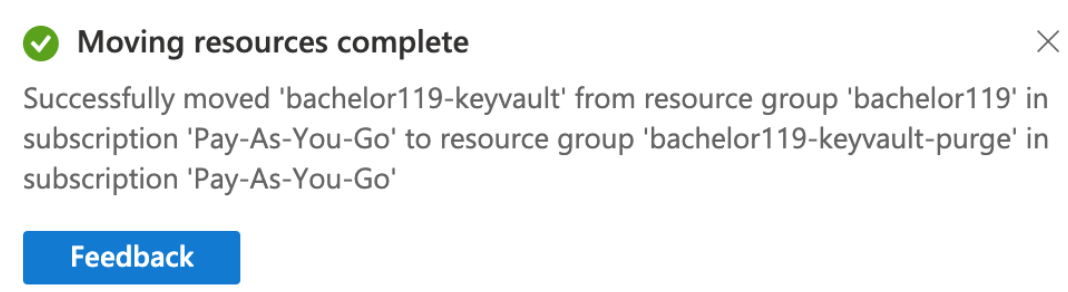
\includegraphics[scale=0.5]{figures/migrate-resource-success.png}

Now it would be interesting to find out what happens when migrating the key vault to a resource group and deleting said group. Testing this out by deleting the resource resource group and the key vault:

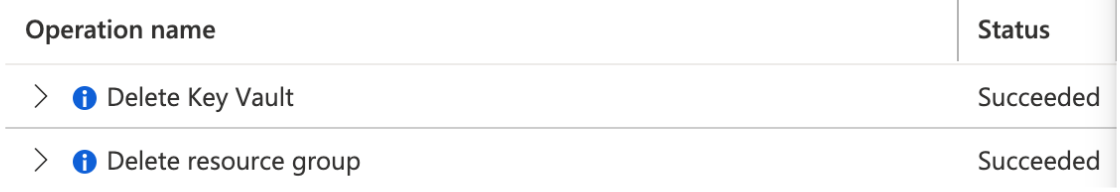
\includegraphics[scale=0.5]{figures/delete-group.png}

Managing deleted key vaults allows the recovery of the key vault. This actions also recreates the previously deleted resource group.

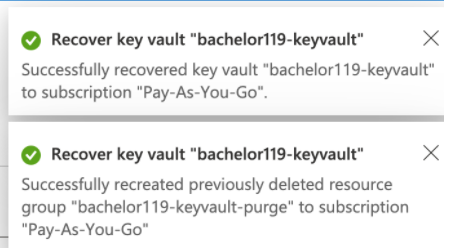
\includegraphics[scale=1.3]{figures/recover-vault.png}

This establishes that purge protection is a safe mechanism for ensuring key vaults regardless of resource group environment. It can not be deleted before the retention period has passed.

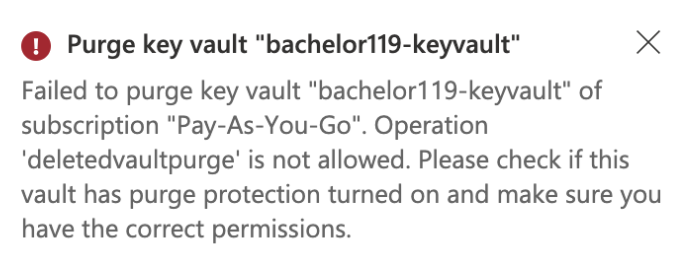
\includegraphics[scale=.8]{figures/purge-denied.png}

It is worth noting that attempting the resource migration and deletion action on a backup vault will not work. In this case the backup vault can not be deleted since it has an active instance being backed up. 

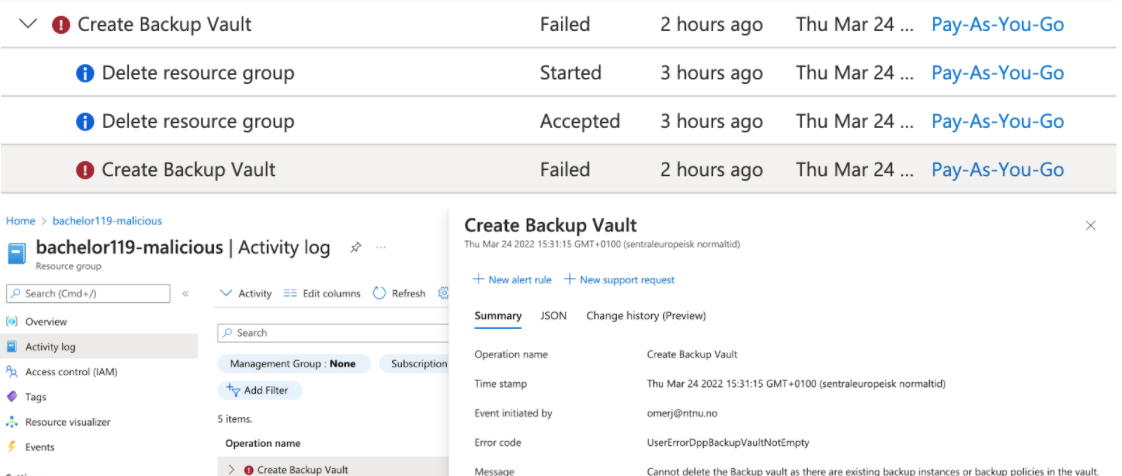
\includegraphics[scale=.7]{figures/backup-migration.png}

\subsection{Deleting a backup vault}
%Worth looking into resource guard here
To delete a resource group with a backup vault:
\begin{enumerate}
    \item Suspend backups of backup instance
    \item Delete backup instance
    \item Delete backup policy
    \item Delete backup vault
    \item Delete resource group
\end{enumerate}
 Each step is is a prerequisite for the next one. You can not delete a backup instance if it is in use, meaning not suspended. You can not delete a backup policy if there is an instance using that policy. The same goes for policy in vault and vault in resource group.

% Backup vault for a postgreSQL flexible server. Set up with data
% Set up policy. Delete database and restore from backup. Record time it takes.
% 

% Can you somehow delete all backups as well?
% Test the same with resource guard.
%
%TODO first thing: Migrate data.

%flexible can restore to a different Vnet while single can only restore to the same one.

%Can you use backup vault for Azure Database for PostgreSQL single server?

%If not, what options are there?

%Test out option. Compare to flexible server restore time.

%Should I add a read replica for PostgreSQL single server?
%write a bit about different ways of backing uup
%https://www.postgresql.org/docs/current/backup.html#:~:text=There%20are%20three%20fundamentally%20different,Continuous%20archiving

\section{Multi-User Authenication takeover}
Unlikely?
Requires 2 specific accounts.


\chapter*{\bibname}
\printbibliography[heading=none]

% First paper

% \begin{paper}{papers/landes1951scrutiny.pdf}{paper:scrutiny}
%     Here, you may add a description of the paper, an illustration, or just give the bibliographic reference:
%     \begin{quote}
%         \fullcite{landes1951scrutiny}
%     \end{quote}
%     Or you may leave it empty, if you like.
% \end{paper}

% Second paper etc.

\appendix

\chapter{Experiment Data}
\label{app:experiment}

This section contains details about how experiments related to the
analysis were performed, as well as results.


% Additional material that does not fit in the main thesis but may still be relevant to share, e.g., raw data from experiments and surveys, code listings, additional plots, pre-project reports, project agreements, contracts, logs etc., can be put in appendices. Simply issue the command \texttt{\textbackslash appendix} in the main \texttt{.tex} file, and make one chapter per appendix.

% If the appendix is in the form of a ready-made PDF file, it should be supported by a small descriptive text, and included using the \texttt{pdfpages} package. To illustrate how it works, a standard project agreement (for the IE faculty at NTNU in Gjøvik) is attached here. You would probably want the included PDF file to begin on an odd (right hand) page, which is achieved by using the \texttt{\textbackslash cleardoublepage} command immediately before the \texttt{\textbackslash includepdf[]\{\}} command. Use the option \texttt{[pages=-]} to include all pages of the PDF document, or, e.g., \texttt{[pages=2-4]} to include only the given page range.

\cleardoublepage
%\includepdf[pages=-]{appendices/NTNUProsjektavtale.pdf}
 \section{Setup of test environment for ClickHouse experiments} 
\label{app:ch-non-perf}
This section contains documentation for how our ClickHouse test environment was set up
in accordance with the specifications listed in the Method chapter (see \ref{method:ch-non-perf}).
This test environment was used for tests that were not performance sensitive.

Most commands were run in the Azure Cloud Shell.
Instead of using the bash environment for the Azure CLI,
we used the PowerShell environment.
Backticks (\texttt{`}) are therefore used instead of backslashes (\texttt{\textbackslash{}}) to escape newlines.

\subsection{Declare variables}
\label{sec:org92d6807}
The following variables were declared to make scripts more reusable:
\begin{minted}[breaklines=true,breakanywhere=true]{powershell}
$AzCloudUser = "torstein"        # Name of Azure user used for CLI commands
$RGName = "testRG"               # Name of resource group
$CHName = "clickhouseVM"         # Name of VM running ClickHouse
$SSHKey = "mySSHKey"             # Name of SSH key used to connect to VM
$SSHPath = "/home/$AzCloudUser/.ssh/$SSHKey.pub"  # Path of SSH keys in Azure Cloud Shell storage
$SAName = "chbksa"               # Name of storage account used by clickhouse-backup
$ContainerName = "chbkcontainer" # Name of container storing clickhouse-backup data
$StagingSAName = "stagingchsa"   # Name of storage account used for Azure Backup staging
$SASExpDate = "2022-05-05"       # Expiry date of SAS token used by clickhouse-backup
$location = "eastus"             # Location of Azure resources
$RSVName = "myRSV"               # Name of Recovery Services Vault
$subscription = "4b48eb85-91f3-4902-b74b-e84641fb6785"  # Subscription ID
$PolicyName = "DefaultPolicy"    # Policy to be used by Azure Backup
\end{minted}

These variables were loaded the other (non-performance) experiments as well.

\subsection{Generate SSH keys}
\label{sec:org07a6fff}
In order to connect to the VM via SSH, SSH keys needed to be generated.

\begin{minted}[breaklines=true,breakanywhere=true]{powershell}
az sshkey create --name $SSHKey --resource-group $RGName
\end{minted}

Output:

\begin{minted}[breaklines=true,breakanywhere=true]{text}
No public key is provided. A key pair is being generated for you.
Private key is saved to "/home/torstein/.ssh/1650965634_7008111".
Public key is saved to "/home/torstein/.ssh/1650965634_7008111.pub".
\end{minted}

\begin{minted}[breaklines=true,breakanywhere=true]{json}
{
  "id": "/subscriptions/4b48eb85-91f3-4902-b74b-e84641fb6785/resourceGroups/TESTRG/providers/Microsoft.Compute/sshPublicKeys/mySSHKey",
  "location": "eastus",
  "name": "mySSHKey",
  "publicKey": "ssh-rsa AAAAB3NzaC1yc2EAAAADAQABAAABgQC4N1FPh8lylHaF1Y2BpTCNNYkO\r\nJ0aaMLSklwBzdA4MrLY0vqnIhJY1QzB7NC3tOxOAqEZVQjqiOiFQRZu0ifV91odi\r\njwuEOWCWia8Wix0AKpxPlFIcUbWE4auf6KOSAAuoTCuXp3H29H+tGtuy/l1ZjBJb\r\nazxFz32j9uwEjVLtkYiYtSPxtnhuTnN6l5wkI36mxni6dQsTKQNTck4bmkU+BmSI\r\nQ4k5YXfhxV0UTqYL5WeVzVDTJnBrDFu8fClio/kcbhCn+w6B2yWfNFuvLmOlpIA6\r\nVZm4MaWpD9mp25J9YDcJ/Y5MewuNW7QqVNQDKfTrWXKz+blkKQ9DVzXvF63myNtQ\r\niMJdzLTvAbgTL0zXPw111r5x8KKHW0nCehWtKvHk2xh2sOcdSVSDu4uZN6eacAPC\r\n4Ii3rJ3QgjL1IxRTITBJ/oZAFxxFZCtPbPYF9pD2iURzibAvLkp5BhLwk954So8G\r\nMzRvVUnM7gtaVNL4UxCYHMbvibwkXaNtu2ZWjGU= generated-by-azure\r\n",
  "resourceGroup": "TESTRG",
  "tags": null,
  "type": null
}
\end{minted}

The keys were then renamed:
\begin{minted}[breaklines=true,breakanywhere=true]{powershell}
cd ~/.ssh
mv ./1650965634_7008111 $SSHKey
mv ./1650965634_7008111.pub ($SSHKey + ".pub")
\end{minted}

These files were then copied to a local machine
in order to be able to access virtual machines using SSH.
\subsection{Set up a resource group}
\label{sec:org880946b}
\begin{minted}[breaklines=true,breakanywhere=true]{powershell}
az group create --name $RGName --location $location
\end{minted}

Output:

\begin{minted}[breaklines=true,breakanywhere=true]{json}
{
  "id": "/subscriptions/4b48eb85-91f3-4902-b74b-e84641fb6785/resourceGroups/testRG",
  "location": "eastus",
  "managedBy": null,
  "name": "testRG",
  "properties": {
    "provisioningState": "Succeeded"
  },
  "tags": null,
  "type": "Microsoft.Resources/resourceGroups"
}
\end{minted}
\subsection{Set up a VM}
\label{sec:orgccb5fe2}
Create an Ubuntu VM:
\begin{minted}[breaklines=true,breakanywhere=true]{powershell}
az vm create `
    --resource-group $RGName `
    --name $CHName `
    --image Canonical:UbuntuServer:16.04-LTS:16.04.202109280 `
    --admin-username azureuser `
    --size Standard_B1s `
    --ssh-key-values $SSHPath `
    --public-ip-sku Standard
\end{minted}

Output:
\begin{minted}[breaklines=true,breakanywhere=true]{json}
{
  "fqdns": "",
  "id": "/subscriptions/4b48eb85-91f3-4902-b74b-e84641fb6785/resourceGroups/testRG/providers/Microsoft.Compute/virtualMachines/clickhouseVM",
  "location": "eastus",
  "macAddress": "00-0D-3A-4F-38-61",
  "powerState": "VM running",
  "privateIpAddress": "10.0.0.4",
  "publicIpAddress": "20.127.83.11",
  "resourceGroup": "testRG",
  "zones": ""
}
\end{minted}

\subsection{Install ClickHouse}
\label{sec:org2265ef7}
Commands to install ClickHouse were copied from the installation guide in the ClickHouse documentation 
\cite{noauthor_installation_nodate}.
% [InstallationClickHouseDocs].

\begin{minted}[breaklines=true,breakanywhere=true]{bash}
sudo apt-get install -y apt-transport-https ca-certificates dirmngr
sudo apt-key adv --keyserver hkp://keyserver.ubuntu.com:80 --recv 8919F6BD2B48D754

echo "deb https://packages.clickhouse.com/deb stable main" | sudo tee \
    /etc/apt/sources.list.d/clickhouse.list
sudo apt-get update

sudo apt-get install -y clickhouse-server clickhouse-client

sudo service clickhouse-server start
\end{minted}

The commands were run as \texttt{azureuser} on the ClickHouse VM.
The ClickHouse default user password was left empty.

Upon running \texttt{clickhouse-client}, which is used to interact with the database, the following warnings were printed:
\begin{minted}[breaklines=true,breakanywhere=true]{text}
 * Linux transparent hugepage are set to "always".
 * Linux threads max count is too low.
 * Available memory at server startup is too low (2GiB).
 * Maximum number of threads is lower than 30000. There could be problems with handling a lot of simultaneous queries.
\end{minted}

This is caused by the VM having quite weak hardware.
The dataset we used was small enough,
and the queries we ran were simple enough,
for this now to be an issue.

\subsection{Load test data}
\label{sec:org62af589}
A simple set of test data was retrieved from the ClickHouse website \cite{noauthor_cell_nodate}.
%[CellTowersClickHouse]
The data set contains cell tower data and is around 700MB.
Since this data set is not intended for use in performance sensitive tests,
we determined that it was sufficiently large.

The data was loaded by following the instructions in the documentation.

Load test data:
\begin{minted}[breaklines=true,breakanywhere=true]{bash}
# Download dataset
wget https://datasets.clickhouse.com/cell_towers.csv.xz

# Decompress dataset
xz -d cell_towers.csv.xz

# Load data into clickhouse
clickhouse-client --query \
"CREATE TABLE cell_towers_two
(
    radio Enum8('' = 0, 'CDMA' = 1, 'GSM' = 2, 'LTE' = 3, 'NR' = 4, 'UMTS' = 5),
    mcc UInt16,
    net UInt16,
    area UInt16,
    cell UInt64,
    unit Int16,
    lon Float64,
    lat Float64,
    range UInt32,
    samples UInt32,
    changeable UInt8,
    created DateTime,
    updated DateTime,
    averageSignal UInt8
)
ENGINE = MergeTree ORDER BY (radio, mcc, net, created);"

# Load test data into database
clickhouse-client --query "INSERT INTO cell_towers FORMAT CSVWithNames" < cell_towers.csv
\end{minted}

\subsection{Run test queries}
\label{sec:org19e6a30}
The following test queries were run from \texttt{clickhouse-client} to verify that
the data was loaded correctly.
The results were compared with the results listed in the documentation \cite{noauthor_cell_nodate}.
% [CellTowersClickHouse]

The outputs of queries are shown in comments under the SQL statements.
The \texttt{TabSeparated} format is used because the default output format
contains Unicode characters that are difficult to display when using \LaTeX.

Test query 1:
\begin{minted}[breaklines=true,breakanywhere=true]{sql}
SELECT
    radio,
    count() AS c
FROM cell_towers
GROUP BY radio
ORDER BY c DESC
FORMAT TabSeparated

-- Query id: 067359b9-2a3b-4683-9e85-74a50cd93719
--
-- UMTS    20686487
-- LTE     12101148
-- GSM     9931312
-- CDMA    556344
-- NR      867
--
-- 10 rows in set. Elapsed: 0.205 sec. Processed 43.28 million rows, 86.55 MB (211.56 million rows/s., 423.12 MB/s.)
\end{minted}

Test query 2:
\begin{minted}[breaklines=true,breakanywhere=true]{sql}
SELECT
    mcc,
    count()
FROM cell_towers
GROUP BY mcc
ORDER BY count() DESC
LIMIT 10
FORMAT TabSeparated

-- Query id: 6f1c8ef2-f866-48d5-b521-abde9d34a65c
--
-- 310     5024650
-- 262     2622423
-- 250     1953176
-- 208     1891187
-- 724     1836150
-- 404     1729151
-- 234     1618924
-- 510     1353998
-- 440     1343355
-- 311     1332798
--
-- 10 rows in set. Elapsed: 0.397 sec. Processed 43.28 million rows, 86.55 MB (108.92 million rows/s., 217.84 MB/s.)
\end{minted}

The results of both queries matched the results in the documentation.

\subsection{Install \texttt{clickhouse-backup}}
\label{sec:org7ea2ed5}
The most recent (as of 2022-05-02) \texttt{clickhouse-backup} binary was downloaded
from \texttt{clickhouse-backup}'s GitHub page \cite{akulov_clickhouse-backup_2022}.
% [akulovClickhousebackup2022]

\begin{minted}[breaklines=true,breakanywhere=true]{bash}
# Download archive containing binary
wget https://github.com/AlexAkulov/clickhouse-backup/releases/download/v1.3.2/clickhouse-backup-linux-amd64.tar.gz

# Decompress archive
tar -zxvf clickhouse-backup-linux-amd64.tar.gz

# Move binary to home directory
mv build/linux/amd64/clickhouse-backup ~

# Cleanup
rmdir -p build/linux/amd64
rm clickhouse-backup-linux-amd64.tar.gz
\end{minted}
\subsection{Set up Azure Blob storage for use with \texttt{clickhouse-backup}}
\label{sec:org929d868}
\texttt{clickhouse-backup} can store remote backups in Azure Blob Storage.
This requires an Azure Storage Account and a Storage Container,
which we created by following the instructions in the Azure documentation \cite{stevenmatthew_quickstart_nodate}
% [stevenmatthewQuickstartUploadDownload]

\subsubsection{Create a storage account}
\label{sec:org292fd33}
Create storage account:
\begin{minted}[breaklines=true,breakanywhere=true]{powershell}
az storage account create `
    --name $SAName `
    --resource-group $RGName `
    --location eastus `
    --sku Standard_LRS `
    --encryption-services blob
\end{minted}

Output:
\begin{minted}[breaklines=true,breakanywhere=true]{json}
{
  "accessTier": "Hot",
  "allowBlobPublicAccess": true,
  "allowCrossTenantReplication": null,
  "allowSharedKeyAccess": null,
  "allowedCopyScope": null,
  "azureFilesIdentityBasedAuthentication": null,
  "blobRestoreStatus": null,
  "creationTime": "2022-04-30T10:14:26.700057+00:00",
  "customDomain": null,
  "defaultToOAuthAuthentication": null,
  "dnsEndpointType": null,
  "enableHttpsTrafficOnly": true,
  "enableNfsV3": null,
  "encryption": {
    "encryptionIdentity": null,
    "keySource": "Microsoft.Storage",
    "keyVaultProperties": null,
    "requireInfrastructureEncryption": null,
    "services": {
      "blob": {
        "enabled": true,
        "keyType": "Account",
        "lastEnabledTime": "2022-04-30T10:14:26.825032+00:00"
      },
      "file": {
        "enabled": true,
        "keyType": "Account",
        "lastEnabledTime": "2022-04-30T10:14:26.825032+00:00"
      },
      "queue": null,
      "table": null
    }
  },
  "extendedLocation": null,
  "failoverInProgress": null,
  "geoReplicationStats": null,
  "id": "/subscriptions/4b48eb85-91f3-4902-b74b-e84641fb6785/resourceGroups/testRG/providers/Microsoft.Storage/storageAccounts/chbksa",
  "identity": null,
  "immutableStorageWithVersioning": null,
  "isHnsEnabled": null,
  "isLocalUserEnabled": null,
  "isSftpEnabled": null,
  "keyCreationTime": {
    "key1": "2022-04-30T10:14:26.825032+00:00",
    "key2": "2022-04-30T10:14:26.825032+00:00"
  },
  "keyPolicy": null,
  "kind": "StorageV2",
  "largeFileSharesState": null,
  "lastGeoFailoverTime": null,
  "location": "eastus",
  "minimumTlsVersion": "TLS1_0",
  "name": "chbksa",
  "networkRuleSet": {
    "bypass": "AzureServices",
    "defaultAction": "Allow",
    "ipRules": [],
    "resourceAccessRules": null,
    "virtualNetworkRules": []
  },
  "primaryEndpoints": {
    "blob": "https://chbksa.blob.core.windows.net/",
    "dfs": "https://chbksa.dfs.core.windows.net/",
    "file": "https://chbksa.file.core.windows.net/",
    "internetEndpoints": null,
    "microsoftEndpoints": null,
    "queue": "https://chbksa.queue.core.windows.net/",
    "table": "https://chbksa.table.core.windows.net/",
    "web": "https://chbksa.z13.web.core.windows.net/"
  },
  "primaryLocation": "eastus",
  "privateEndpointConnections": [],
  "provisioningState": "Succeeded",
  "publicNetworkAccess": null,
  "resourceGroup": "testRG",
  "routingPreference": null,
  "sasPolicy": null,
  "secondaryEndpoints": null,
  "secondaryLocation": null,
  "sku": {
    "name": "Standard_LRS",
    "tier": "Standard"
  },
  "statusOfPrimary": "available",
  "statusOfSecondary": null,
  "storageAccountSkuConversionStatus": null,
  "tags": {},
  "type": "Microsoft.Storage/storageAccounts"
}
\end{minted}

\subsubsection{Create a storage container}
\label{sec:org11db3a7}
Create storage container:
\begin{minted}[breaklines=true,breakanywhere=true]{powershell}
az storage container create `
    --account-name $SAName `
    --name $ContainerName `
    --auth-mode login
\end{minted}

Output:
\begin{minted}[breaklines=true,breakanywhere=true]{json}
{
  "created": true
}
\end{minted}
\subsection{Enable soft delete for Blob container}
\label{sec:orgd26843b}
Enable soft delete for Blob container:
\begin{minted}[breaklines=true,breakanywhere=true]{powershell}
az storage account blob-service-properties update `
    --enable-container-delete-retention true `
    --container-delete-retention-days 7 `
    --account-name $SAName `
    --resource-group $RGName
\end{minted}

Output:
\begin{minted}[breaklines=true,breakanywhere=true]{json}
{
  "automaticSnapshotPolicyEnabled": null,
  "changeFeed": null,
  "containerDeleteRetentionPolicy": {
    "allowPermanentDelete": null,
    "days": 7,
    "enabled": true
  },
  "cors": {
    "corsRules": []
  },
  "defaultServiceVersion": null,
  "deleteRetentionPolicy": {
    "allowPermanentDelete": false,
    "days": null,
    "enabled": false
  },
  "id": "/subscriptions/4b48eb85-91f3-4902-b74b-e84641fb6785/resourceGroups/testRG/providers/Microsoft.Storage/storageAccounts/chbksa/blobServices/default",
  "isVersioningEnabled": null,
  "lastAccessTimeTrackingPolicy": null,
  "name": "default",
  "resourceGroup": "testRG",
  "restorePolicy": null,
  "sku": null,
  "type": "Microsoft.Storage/storageAccounts/blobServices"
}
\end{minted}
\subsection{Configure \texttt{clickhouse-backup} to use Blob storage}
\label{sec:org8552124}
\subsubsection{Generate \texttt{clickkhouse-backup} configuration file}
\label{sec:org2c08657}
A configuration file for \texttt{clickhouse-backup} was generated with
\texttt{sudo ./clickhouse-backup default-config > config.yaml}

\begin{minted}[breaklines=true,breakanywhere=true]{yaml}
general:
  remote_storage: none
  max_file_size: 0
  disable_progress_bar: true
  backups_to_keep_local: 0
  backups_to_keep_remote: 0
  log_level: info
  allow_empty_backups: false
  download_concurrency: 1
  upload_concurrency: 1
  restore_schema_on_cluster: ""
  upload_by_part: true
  download_by_part: true
clickhouse:
  username: default
  password: ""
  host: localhost
  port: 9000
  disk_mapping: {}
  skip_tables:
  - system.*
  - INFORMATION_SCHEMA.*
  - information_schema.*
  timeout: 5m
  freeze_by_part: false
  secure: false
  skip_verify: false
  sync_replicated_tables: false
  log_sql_queries: true
  config_dir: /etc/clickhouse-server/
  restart_command: systemctl restart clickhouse-server
  ignore_not_exists_error_during_freeze: true
  tls_key: ""
  tls_cert: ""
  tls_ca: ""
  debug: false
s3:
  access_key: ""
  secret_key: ""
  bucket: ""
  endpoint: ""
  region: us-east-1
  acl: private
  assume_role_arn: ""
  force_path_style: false
  path: ""
  disable_ssl: false
  compression_level: 1
  compression_format: tar
  sse: ""
  disable_cert_verification: false
  storage_class: STANDARD
  concurrency: 1
  part_size: 0
  max_parts_count: 10000
  debug: false
gcs:
  credentials_file: ""
  credentials_json: ""
  bucket: ""
  path: ""
  compression_level: 1
  compression_format: tar
  debug: false
  endpoint: ""
cos:
  url: ""
  timeout: 2m
  secret_id: ""
  secret_key: ""
  path: ""
  compression_format: tar
  compression_level: 1
  debug: false
api:
  listen: localhost:7171
  enable_metrics: true
  enable_pprof: false
  username: ""
  password: ""
  secure: false
  certificate_file: ""
  private_key_file: ""
  create_integration_tables: false
  allow_parallel: false
ftp:
  address: ""
  timeout: 2m
  username: ""
  password: ""
  tls: false
  path: ""
  compression_format: tar
  compression_level: 1
  concurrency: 1
  debug: false
sftp:
  address: ""
  port: 22
  username: ""
  password: ""
  key: ""
  path: ""
  compression_format: tar
  compression_level: 1
  concurrency: 1
  debug: false
azblob:
  endpoint_suffix: core.windows.net
  account_name: ""
  account_key: ""
  sas: ""
  use_managed_identity: false
  container: ""
  path: ""
  compression_level: 1
  compression_format: tar
  sse_key: ""
  buffer_size: 0
  buffer_count: 3
  max_parts_count: 0
\end{minted}

\subsubsection{Get necessary config details}
\label{sec:org287aa3d}
In order to configure \texttt{clickhouse-backup} for use with Azure Storage Blobs,
we need an access key and a SAS token.

\begin{enumerate}
\item Get access key for storage account
\label{sec:org9615db0}
\begin{minted}[breaklines=true,breakanywhere=true]{powershell}
az storage account keys list `
  --resource-group $RGName `
  --account-name $SAName
\end{minted}

Output:
\begin{minted}[breaklines=true,breakanywhere=true]{json}
[
  {
    "creationTime": "2022-04-30T10:14:26.825032+00:00",
    "keyName": "key1",
    "permissions": "FULL",
    "value": "NdbW07WlHBf5zcpMXundwkP88Ie2SO1Ad+84VD8moaUg1ihIeRR7cEdy4FXIgHRvIQwPIMc7eD2q+ASt6EqxWg=="
  },
  {
    "creationTime": "2022-04-30T10:14:26.825032+00:00",
    "keyName": "key2",
    "permissions": "FULL",
    "value": "vs33au0M52gdtKdhqeOiC0vBGRRqO1qUtvQk0Eg2c4TVIFHETmWR7taS8w2ZU5mEAPzYS4ySWBXY+AStcBusiQ=="
  }
]
\end{minted}

\item Get SAS token for container
\label{sec:org6e529f4}
\begin{minted}[breaklines=true,breakanywhere=true]{powershell}
az storage container generate-sas `
    --account-name $SAName `
    --name $ContainerName `
    --permissions acdlrw `
    --expiry $SASExpDate `
    --auth-mode login `
    --as-user
\end{minted}

Output:
\begin{minted}[breaklines=true,breakanywhere=true]{text}
"se=2022-05-05&sp=racwdl&sv=2021-04-10&sr=c&skoid=d404139d-e156-421c-9450-19e9734a8141&sktid=09a10672-822f-4467-a5ba-5bb375967c05&skt=2022-04-30T10%3A32%3A05Z&ske=2022-05-05T00%3A00%3A00Z&sks=b&skv=2021-04-10&sig=CoeOsK63ZSnuqUqn%2Bv2ZgE9/sELwp/Hinxj6abW9qfo%3D"
\end{minted}
\end{enumerate}

\subsubsection{Modify configuration file to make it work with Blob storage}
\label{sec:org513a57f}
Some \texttt{general} settings were modified:
\begin{itemize}
\item \texttt{remote\_storage} was set to \texttt{azblob} (from \texttt{none}).
\item \texttt{max\_parts\_count} was set to 1 (from 0).
\item \texttt{disable\_progress\_bar} was set to \texttt{false} (from \texttt{true}).
\end{itemize}

The necessary \texttt{azblob} details were also filled in.

Modified version of \texttt{config.yaml}:
\begin{minted}[breaklines=true,breakanywhere=true]{yaml}
general:
  remote_storage: azblob
  max_file_size: 0
  disable_progress_bar: false
  backups_to_keep_local: 0
  backups_to_keep_remote: 0
  log_level: info
  allow_empty_backups: false
  download_concurrency: 1
  upload_concurrency: 1
  restore_schema_on_cluster: ""
  upload_by_part: true
  download_by_part: true
clickhouse:
  username: default
  password: ""
  host: localhost
  port: 9000
  disk_mapping: {}
  skip_tables:
  - system.*
  - INFORMATION_SCHEMA.*
  - information_schema.*
  timeout: 5m
  freeze_by_part: false
  secure: false
  skip_verify: false
  sync_replicated_tables: false
  log_sql_queries: true
  config_dir: /etc/clickhouse-server/
  restart_command: systemctl restart clickhouse-server
  ignore_not_exists_error_during_freeze: true
  tls_key: ""
  tls_cert: ""
  tls_ca: ""
  debug: false
s3:
  access_key: ""
  secret_key: ""
  bucket: ""
  endpoint: ""
  region: us-east-1
  acl: private
  assume_role_arn: ""
  force_path_style: false
  path: ""
  disable_ssl: false
  compression_level: 1
  compression_format: tar
  sse: ""
  disable_cert_verification: false
  storage_class: STANDARD
  concurrency: 1
  part_size: 0
  max_parts_count: 10000
  debug: false
gcs:
  credentials_file: ""
  credentials_json: ""
  bucket: ""
  path: ""
  compression_level: 1
  compression_format: tar
  debug: false
  endpoint: ""
cos:
  url: ""
  timeout: 2m
  secret_id: ""
  secret_key: ""
  path: ""
  compression_format: tar
  compression_level: 1
  debug: false
api:
  listen: localhost:7171
  enable_metrics: true
  enable_pprof: false
  username: ""
  password: ""
  secure: false
  certificate_file: ""
  private_key_file: ""
  create_integration_tables: false
  allow_parallel: false
ftp:
  address: ""
  timeout: 2m
  username: ""
  password: ""
  tls: false
  path: ""
  compression_format: tar
  compression_level: 1
  concurrency: 1
  debug: false
sftp:
  address: ""
  port: 22
  username: ""
  password: ""
  key: ""
  path: ""
  compression_format: tar
  compression_level: 1
  concurrency: 1
  debug: false
azblob:
  endpoint_suffix: core.windows.net
  account_name: "chbksa"
  account_key: "NdbW07WlHBf5zcpMXundwkP88Ie2SO1Ad+84VD8moaUg1ihIeRR7cEdy4FXIgHRvIQwPIMc7eD2q+ASt6EqxWg=="
  sas: "?sv=2020-08-04&ss=bfqt&srt=c&sp=rwdlacupitfx&se=2022-05-02T14:36:42Z&st=2022-05-02T06:36:42Z&spr=https&sig=ONxr9dN3ayvlq1fwk4b516u%2F9X1ZjVNamV88yeeYksU%3D"
  use_managed_identity: false
  container: "chbkcontainer"
  path: "https://chbksa.blob.core.windows.net/chbkcontainer"
  compression_level: 1
  compression_format: tar
  sse_key: ""
  buffer_size: 0
  buffer_count: 3
  max_parts_count: 1
\end{minted}

\subsubsection{Perform local backup}
\label{sec:orgfb658c8}
Create a local backup:
\begin{minted}[breaklines=true,breakanywhere=true]{bash}
sudo ./clickhouse-backup create

# 2022/05/02 09:34:00.837899  info SELECT name, engine FROM system.databases WHERE name NOT IN ('system', 'INFORMATION_SCHEMA', 'information_schema')
# 2022/05/02 09:34:00.844477  info SHOW CREATE DATABASE `default`
# 2022/05/02 09:34:00.849781  info SELECT count() FROM system.settings WHERE name = 'show_table_uuid_in_table_create_query_if_not_nil'
# 2022/05/02 09:34:00.861793  info SELECT name FROM system.databases WHERE engine IN ('MySQL','PostgreSQL')
# 2022/05/02 09:34:00.867246  info
# 		SELECT
# 			countIf(name='data_path') is_data_path_present,
# 			countIf(name='data_paths') is_data_paths_present,
# 			countIf(name='uuid') is_uuid_present,
# 			countIf(name='create_table_query') is_create_table_query_present,
# 			countIf(name='total_bytes') is_total_bytes_present
# 		FROM system.columns WHERE database='system' AND table='tables'
#
# 2022/05/02 09:34:00.881984  info SELECT database, name, engine , data_paths , uuid , create_table_query , coalesce(total_bytes, 0) AS total_bytes   FROM system.tables WHERE is_temporary = 0 SETTINGS show_table_uuid_in_table_create_query_if_not_nil=1
# 2022/05/02 09:34:00.911828  info SELECT value FROM `system`.`build_options` where name='VERSION_INTEGER'
# 2022/05/02 09:34:00.920436  info SELECT * FROM system.disks;
# 2022/05/02 09:34:00.929018  info ALTER TABLE `default`.`cell_towers` FREEZE WITH NAME '671596e8b89e4fc4bc4b69c4992011d4';
# 2022/05/02 09:34:01.002079  info done                      backup=2022-05-02T09-34-00 operation=create table=default.cell_towers
# 2022/05/02 09:34:01.002456  info SELECT value FROM `system`.`build_options` where name='VERSION_DESCRIBE'
# 2022/05/02 09:34:01.008365  info done                      backup=2022-05-02T09-34-00 duration=173ms operation=create
\end{minted}

List local backups:
\begin{minted}[breaklines=true,breakanywhere=true]{bash}
sudo ./clickhouse-backup list

# 2022/05/02 09:36:01.867327  info SELECT value FROM `system`.`build_options` where name='VERSION_INTEGER'
# 2022/05/02 09:36:01.871571  info SELECT * FROM system.disks;
# 2022-05-02T09-34-00   1.07GiB   02/05/2022 09:34:01   local
\end{minted}

\subsubsection{Perform remote backup}
\label{sec:orgbcc25d0}
Create a remote backup:
\begin{minted}[breaklines=true,breakanywhere=true]{bash}
sudo ./clickhouse-backup create_remote --config config.yaml

# 2022/05/02 09:48:18.613252  info SELECT name, engine FROM system.databases WHERE name NOT IN ('system', 'INFORMATION_SCHEMA', 'information_schema')
# 2022/05/02 09:48:18.616953  info SHOW CREATE DATABASE `default`
# 2022/05/02 09:48:18.619861  info SELECT count() FROM system.settings WHERE name = 'show_table_uuid_in_table_create_query_if_not_nil'
# 2022/05/02 09:48:18.622844  info SELECT name FROM system.databases WHERE engine IN ('MySQL','PostgreSQL')
# 2022/05/02 09:48:18.625686  info
# 		SELECT
# 			countIf(name='data_path') is_data_path_present,
# 			countIf(name='data_paths') is_data_paths_present,
# 			countIf(name='uuid') is_uuid_present,
# 			countIf(name='create_table_query') is_create_table_query_present,
# 			countIf(name='total_bytes') is_total_bytes_present
# 		FROM system.columns WHERE database='system' AND table='tables'
#
# 2022/05/02 09:48:18.633230  info SELECT database, name, engine , data_paths , uuid , create_table_query , coalesce(total_bytes, 0) AS total_bytes   FROM system.tables WHERE is_temporary = 0 SETTINGS show_table_uuid_in_table_create_query_if_not_nil=1
# 2022/05/02 09:48:18.642818  info SELECT value FROM `system`.`build_options` where name='VERSION_INTEGER'
# 2022/05/02 09:48:18.648335  info SELECT * FROM system.disks;
# 2022/05/02 09:48:18.652902  info ALTER TABLE `default`.`cell_towers` FREEZE WITH NAME '005688e38c3e41dfa2da8d275e7d3c2b';
# 2022/05/02 09:48:18.736020  info done                      backup=2022-05-02T09-48-18 operation=create table=default.cell_towers
# 2022/05/02 09:48:18.736333  info SELECT value FROM `system`.`build_options` where name='VERSION_DESCRIBE'
# 2022/05/02 09:48:18.741265  info done                      backup=2022-05-02T09-48-18 duration=132ms operation=create
# 2022/05/02 09:48:18.747950  info SELECT value FROM `system`.`build_options` where name='VERSION_INTEGER'
# 2022/05/02 09:48:18.752206  info SELECT * FROM system.disks;
# 2022/05/02 09:48:18.758250  info SELECT max(toInt64(bytes_on_disk * 1.02)) AS max_file_size FROM system.parts
# 2022/05/02 09:48:39.787095  info done                      backup=2022-05-02T09-48-18 duration=20.971s operation=upload size=1.07GiB table=default.cell_towers
# 2022/05/02 09:48:39.804194  info done                      backup=2022-05-02T09-48-18 duration=21.063s operation=upload size=1.07GiB
\end{minted}

List remote backups:
\begin{minted}[breaklines=true,breakanywhere=true]{bash}
sudo ./clickhouse-backup list remote --config config.yaml

# 2022/05/02 09:53:50.813272  info SELECT max(toInt64(bytes_on_disk * 1.02)) AS max_file_size FROM system.parts
# 2022-05-02T09-48-18   1.07GiB   02/05/2022 09:48:39   remote      tar
\end{minted}

The backup was also visible in the Azure Portal.

\subsection{Set up Azure Backup}
\label{sec:org6963b1d}
Azure Backup was set up to back up the ClickHouse VM.
Commands are mostly based on instructions from the Azure Documentation \cite{v-amallick_quickstart_nodate}
% [v-amallickQuickstartBackVM]

\subsubsection{Create a Recovery Services vault}
\label{sec:org05625d6}
\begin{minted}[breaklines=true,breakanywhere=true]{powershell}
az backup vault create --location $location --name $RSVName --resource-group $RGName
\end{minted}

Output:
\begin{minted}[breaklines=true,breakanywhere=true]{json}
{
  "etag": "W/\"datetime'2022-05-02T12%3A34%3A13.452294Z'\"",
  "id": "/subscriptions/4b48eb85-91f3-4902-b74b-e84641fb6785/resourceGroups/testRG/providers/Microsoft.RecoveryServices/vaults/myRSV",
  "identity": null,
  "location": "eastus",
  "name": "myRSV",
  "properties": {
    "encryption": null,
    "privateEndpointConnections": null,
    "privateEndpointStateForBackup": "None",
    "privateEndpointStateForSiteRecovery": "None",
    "provisioningState": "Succeeded",
    "upgradeDetails": null
  },
  "resourceGroup": "testRG",
  "sku": {
    "name": "Standard",
    "tier": null
  },
  "systemData": null,
  "tags": null,
  "type": "Microsoft.RecoveryServices/vaults"
}
\end{minted}

\subsubsection{Disable geo-redundancy}
\label{sec:orgf8d56a4}
To save on costs, we disabled geo-redundant storage.

\begin{minted}[breaklines=true,breakanywhere=true]{powershell}
az backup vault backup-properties set --backup-storage-redundancy LocallyRedundant --name $RSVName --resource-group $RGName --subscription $subscription
\end{minted}

Output:
\begin{minted}[breaklines=true,breakanywhere=true]{json}
{
  "eTag": null,
  "id": "/subscriptions/4b48eb85-91f3-4902-b74b-e84641fb6785/resourceGroups/testRG/providers/Microsoft.RecoveryServices/vaults/myRSV/backupstorageconfig/vaultstorageconfig",
  "location": null,
  "name": "vaultstorageconfig",
  "properties": {
    "crossRegionRestoreFlag": false,
    "dedupState": "Disabled",
    "storageModelType": "LocallyRedundant",
    "storageType": "LocallyRedundant",
    "storageTypeState": "Unlocked",
    "xcoolState": "Disabled"
  },
  "resourceGroup": "testRG",
  "tags": null,
  "type": "Microsoft.RecoveryServices/vaults/backupstorageconfig"
}
\end{minted}
\subsubsection{Decide which backup policy to use}
\label{sec:orgbd40151}
We determined that the default policy is sufficient for our experiments.
The policy is listed below.

\begin{minted}[breaklines=true,breakanywhere=true]{powershell}
az backup policy show -g $RGName -v $RSVName -n DefaultPolicy
\end{minted}

Output:
\begin{minted}[breaklines=true,breakanywhere=true]{json}
{
  "eTag": null,
  "id": "/subscriptions/4b48eb85-91f3-4902-b74b-e84641fb6785/resourceGroups/testRG/providers/Microsoft.RecoveryServices/vaults/myRSV/backupPolicies/DefaultPolicy",
  "location": null,
  "name": "DefaultPolicy",
  "properties": {
    "backupManagementType": "AzureIaasVM",
    "instantRpDetails": {
      "azureBackupRgNamePrefix": null,
      "azureBackupRgNameSuffix": null
    },
    "instantRpRetentionRangeInDays": 2,
    "policyType": null,
    "protectedItemsCount": 0,
    "resourceGuardOperationRequests": null,
    "retentionPolicy": {
      "dailySchedule": {
        "retentionDuration": {
          "count": 30,
          "durationType": "Days"
        },
        "retentionTimes": [
          "2022-05-02T20:00:00+00:00"
        ]
      },
      "monthlySchedule": null,
      "retentionPolicyType": "LongTermRetentionPolicy",
      "weeklySchedule": null,
      "yearlySchedule": null
    },
    "schedulePolicy": {
      "hourlySchedule": null,
      "schedulePolicyType": "SimpleSchedulePolicy",
      "scheduleRunDays": null,
      "scheduleRunFrequency": "Daily",
      "scheduleRunTimes": [
        "2022-05-02T20:00:00+00:00"
      ],
      "scheduleWeeklyFrequency": 0
    },
    "timeZone": "UTC"
  },
  "resourceGroup": "testRG",
  "tags": null,
  "type": "Microsoft.RecoveryServices/vaults/backupPolicies"
}
\end{minted}
\subsubsection{Enable backup for the VM}
\label{sec:org3803369}
\begin{minted}[breaklines=true,breakanywhere=true]{powershell}
az backup protection enable-for-vm `
 --resource-group $RGName `
 --vault-name $RSVName `
 --vm $CHName `
 --policy-name $PolicyName
\end{minted}

Output:
\begin{minted}[breaklines=true,breakanywhere=true]{json}
{
  "eTag": null,
  "id": "/subscriptions/4b48eb85-91f3-4902-b74b-e84641fb6785/resourceGroups/testRG/providers/Microsoft.RecoveryServices/vaults/myRSV/backupJobs/a09a2633-ec57-43c5-b121-b48d19cd936a",
  "location": null,
  "name": "a09a2633-ec57-43c5-b121-b48d19cd936a",
  "properties": {
    "actionsInfo": null,
    "activityId": "62452fde-ca14-11ec-a1e3-0a580af43d64",
    "backupManagementType": "AzureIaasVM",
    "containerName": "iaasvmcontainerv2;testrg;clickhousevm",
    "duration": "0:00:30.954373",
    "endTime": "2022-05-02T12:36:20.005999+00:00",
    "entityFriendlyName": "clickhousevm",
    "errorDetails": null,
    "extendedInfo": {
      "dynamicErrorMessage": null,
      "estimatedRemainingDuration": null,
      "internalPropertyBag": null,
      "progressPercentage": null,
      "propertyBag": {
        "Policy Name": "DefaultPolicy",
        "VM Name": "clickhousevm"
      },
      "tasksList": []
    },
    "isUserTriggered": null,
    "jobType": "AzureIaaSVMJob",
    "operation": "ConfigureBackup",
    "startTime": "2022-05-02T12:35:49.051626+00:00",
    "status": "Completed",
    "virtualMachineVersion": "Compute"
  },
  "resourceGroup": "testRG",
  "tags": null,
  "type": "Microsoft.RecoveryServices/vaults/backupJobs"
}
\end{minted}

\subsubsection{Make a backup of the ClickHouse VM}
\label{sec:org9e0d508}
In order to trigger a backup job instantly, we ran the following:
\begin{minted}[breaklines=true,breakanywhere=true]{powershell}
az backup protection backup-now `
    --resource-group $RGName `
    --vault-name $RSVName `
    --container-name $CHName `
    --item-name $CHName `
    --backup-management-type AzureIaaSVM `
    --retain-until 06-05-2022
\end{minted}

Output:
\begin{minted}[breaklines=true,breakanywhere=true]{json}
{
  "eTag": null,
  "id": "/subscriptions/4b48eb85-91f3-4902-b74b-e84641fb6785/resourceGroups/testRG/providers/Microsoft.RecoveryServices/vaults/myRSV/backupJobs/d52437c1-3ad2-4312-98a7-a75b4eea6e7e",
  "location": null,
  "name": "d52437c1-3ad2-4312-98a7-a75b4eea6e7e",
  "properties": {
    "actionsInfo": [
      "1"
    ],
    "activityId": "950770e4-ca14-11ec-a745-0a580af43d64",
    "backupManagementType": "AzureIaasVM",
    "containerName": "iaasvmcontainerv2;testrg;clickhousevm",
    "duration": "0:00:01.836772",
    "endTime": null,
    "entityFriendlyName": "clickhousevm",
    "errorDetails": null,
    "extendedInfo": {
      "dynamicErrorMessage": null,
      "estimatedRemainingDuration": null,
      "internalPropertyBag": {
        "IsInstantRpJob": "True"
      },
      "progressPercentage": null,
      "propertyBag": {
        "Recovery Point Expiry Time in UTC": "5/6/2022 12:00:00 AM",
        "VM Name": "clickhousevm"
      },
      "tasksList": [
        {
          "duration": "0:00:00",
          "endTime": null,
          "instanceId": null,
          "progressPercentage": null,
          "startTime": null,
          "status": "InProgress",
          "taskExecutionDetails": null,
          "taskId": "Take Snapshot"
        },
        {
          "duration": "0:00:00",
          "endTime": null,
          "instanceId": null,
          "progressPercentage": null,
          "startTime": null,
          "status": "NotStarted",
          "taskExecutionDetails": null,
          "taskId": "Transfer data to vault"
        }
      ]
    },
    "isUserTriggered": null,
    "jobType": "AzureIaaSVMJob",
    "operation": "Backup",
    "startTime": "2022-05-02T12:37:10.978974+00:00",
    "status": "InProgress",
    "virtualMachineVersion": "Compute"
  },
  "resourceGroup": "testRG",
  "tags": null,
  "type": "Microsoft.RecoveryServices/vaults/backupJobs"
}
\end{minted}

 \section{Test environment for ClickHouse performance tests}
\label{app:ch-perf}
Azure CLI commands were run in the Azure Cloud Shell (PowerShell).

Bash commands (the commands run on the VM) were run as \texttt{azureuser}
(the default user) in \path{/home/azureuser}, unless specified otherwise.

SQL queries were run in \texttt{clickhouse-client}.

The VM used had the following specifications:
\begin{itemize}
\item 16 GB of RAM
\item 4 vCPUs
\item 2048GB SSD
\item Ubuntu 16.04
\end{itemize}

The procedure for setting the environment up is generally the same as for the normal test environment
(see [cref]).

\subsection{Declare variables}
\label{sec:org306c306}
The following variables were declared to make scripts more reusable.
They are mostly the same as the normal test environment,
except having ``perf'' (performance) prefixed.

\begin{minted}[breaklines=true,breakanywhere=true]{powershell}
$AzCloudUser = "torstein"        # Name of Azure user used for CLI commands
$RGName = "perfRG"               # Name of resource group
$CHName = "perfClickhouseVM"         # Name of VM running ClickHouse
$SSHKey = "mySSHKey"             # Name of SSH key used to connect to VM
$SSHPath = "/home/$AzCloudUser/.ssh/$SSHKey.pub"  # Path of SSH keys in Azure Cloud Shell storage
$SAName = "perfchbksa"               # Name of storage account used by clickhouse-backup
$ContainerName = "chbkperfcontainer" # Name of container storing clickhouse-backup data
$StagingSAName = "perfstagingchsa"   # Name of storage account used for Azure Backup staging
$SASExpDate = "2022-05-18"       # Expiry date of SAS token used by clickhouse-backup
$location = "eastus"             # Location of Azure resources
$RSVName = "perfRSV"               # Name of Recovery Services Vault
$subscription = "4b48eb85-91f3-4902-b74b-e84641fb6785"  # Subscription ID
$PolicyName = "DefaultPolicy"    # Policy to be used by Azure Backup
\end{minted}
\subsection{Set up a resource group}
\label{sec:orgccc1bce}
Create resource group:
\begin{minted}[breaklines=true,breakanywhere=true]{powershell}
az group create --name $RGName --location $location
\end{minted}

Output:
\begin{minted}[breaklines=true,breakanywhere=true]{json}
{
  "id": "/subscriptions/4b48eb85-91f3-4902-b74b-e84641fb6785/resourceGroups/perfRG",
  "location": "eastus",
  "managedBy": null,
  "name": "perfRG",
  "properties": {
    "provisioningState": "Succeeded"
  },
  "tags": null,
  "type": "Microsoft.Resources/resourceGroups"
}
\end{minted}
\subsection{Set up a VM}
\label{sec:orgc560500}
Create an Ubuntu VM:
\begin{minted}[breaklines=true,breakanywhere=true]{powershell}
az vm create `
    --resource-group $RGName `
    --name $CHName `
    --image Canonical:UbuntuServer:16.04-LTS:16.04.202109280 `
    --admin-username azureuser `
    --size Standard_D4s_v4 `
    --os-disk-size-gb 2048 `
    --ssh-key-values $SSHPath `
    --public-ip-sku Standard
\end{minted}

Output:
\begin{minted}[breaklines=true,breakanywhere=true]{json}
{
  "fqdns": "",
  "id": "/subscriptions/4b48eb85-91f3-4902-b74b-e84641fb6785/resourceGroups/perfRG/providers/Microsoft.Compute/virtualMachines/perfClickhouseVM",
  "location": "eastus",
  "macAddress": "00-22-48-25-AA-BE",
  "powerState": "VM running",
  "privateIpAddress": "10.0.0.4",
  "publicIpAddress": "20.237.81.139",
  "resourceGroup": "perfRG",
  "zones": ""
}
\end{minted}
\subsection{Install ClickHouse}
\label{sec:org963a40c}
Commands to install ClickHouse were copied from the installation guide in the ClickHouse documentation [InstallationClickHouseDocs].
The ClickHouse default user password was left empty.

\begin{minted}[breaklines=true,breakanywhere=true]{bash}
sudo apt-get install -y apt-transport-https ca-certificates dirmngr
sudo apt-key adv --keyserver hkp://keyserver.ubuntu.com:80 --recv 8919F6BD2B48D754

echo "deb https://packages.clickhouse.com/deb stable main" | sudo tee \
    /etc/apt/sources.list.d/clickhouse.list
sudo apt-get update

sudo apt-get install -y clickhouse-server clickhouse-client

sudo service clickhouse-server start
\end{minted}

\subsection{Load test data}
\label{sec:orgf169474}
Followed instructions at
[\url{https://ghe.clickhouse.tech/}]

The compressed size was 200GB when loaded in the database.
The dataset was therefore loaded 5 times into different tables in ClickHouse,
in order to fill the database with 1TB of compressed data.

Commands were run on the VM.

Install tool for decompression:
\begin{minted}[breaklines=true,breakanywhere=true]{bash}
sudo apt install pixz
\end{minted}

Download compressed dataset:
\begin{minted}[breaklines=true,breakanywhere=true]{bash}
wget https://datasets.clickhouse.com/github_events_v2.native.xz
\end{minted}

Create five tables for the data in \texttt{clickhouse-client}:
\begin{minted}[breaklines=true,breakanywhere=true]{sql}
CREATE TABLE github_events1
(
    file_time DateTime,
    event_type Enum('CommitCommentEvent' = 1, 'CreateEvent' = 2, 'DeleteEvent' = 3, 'ForkEvent' = 4,
                    'GollumEvent' = 5, 'IssueCommentEvent' = 6, 'IssuesEvent' = 7, 'MemberEvent' = 8,
                    'PublicEvent' = 9, 'PullRequestEvent' = 10, 'PullRequestReviewCommentEvent' = 11,
                    'PushEvent' = 12, 'ReleaseEvent' = 13, 'SponsorshipEvent' = 14, 'WatchEvent' = 15,
                    'GistEvent' = 16, 'FollowEvent' = 17, 'DownloadEvent' = 18, 'PullRequestReviewEvent' = 19,
                    'ForkApplyEvent' = 20, 'Event' = 21, 'TeamAddEvent' = 22),
    actor_login LowCardinality(String),
    repo_name LowCardinality(String),
    created_at DateTime,
    updated_at DateTime,
    action Enum('none' = 0, 'created' = 1, 'added' = 2, 'edited' = 3, 'deleted' = 4, 'opened' = 5, 'closed' = 6, 'reopened' = 7, 'assigned' = 8, 'unassigned' = 9,
                'labeled' = 10, 'unlabeled' = 11, 'review_requested' = 12, 'review_request_removed' = 13, 'synchronize' = 14, 'started' = 15, 'published' = 16, 'update' = 17, 'create' = 18, 'fork' = 19, 'merged' = 20),
    comment_id UInt64,
    body String,
    path String,
    position Int32,
    line Int32,
    ref LowCardinality(String),
    ref_type Enum('none' = 0, 'branch' = 1, 'tag' = 2, 'repository' = 3, 'unknown' = 4),
    creator_user_login LowCardinality(String),
    number UInt32,
    title String,
    labels Array(LowCardinality(String)),
    state Enum('none' = 0, 'open' = 1, 'closed' = 2),
    locked UInt8,
    assignee LowCardinality(String),
    assignees Array(LowCardinality(String)),
    comments UInt32,
    author_association Enum('NONE' = 0, 'CONTRIBUTOR' = 1, 'OWNER' = 2, 'COLLABORATOR' = 3, 'MEMBER' = 4, 'MANNEQUIN' = 5),
    closed_at DateTime,
    merged_at DateTime,
    merge_commit_sha String,
    requested_reviewers Array(LowCardinality(String)),
    requested_teams Array(LowCardinality(String)),
    head_ref LowCardinality(String),
    head_sha String,
    base_ref LowCardinality(String),
    base_sha String,
    merged UInt8,
    mergeable UInt8,
    rebaseable UInt8,
    mergeable_state Enum('unknown' = 0, 'dirty' = 1, 'clean' = 2, 'unstable' = 3, 'draft' = 4),
    merged_by LowCardinality(String),
    review_comments UInt32,
    maintainer_can_modify UInt8,
    commits UInt32,
    additions UInt32,
    deletions UInt32,
    changed_files UInt32,
    diff_hunk String,
    original_position UInt32,
    commit_id String,
    original_commit_id String,
    push_size UInt32,
    push_distinct_size UInt32,
    member_login LowCardinality(String),
    release_tag_name String,
    release_name String,
    review_state Enum('none' = 0, 'approved' = 1, 'changes_requested' = 2, 'commented' = 3, 'dismissed' = 4, 'pending' = 5)
)
ENGINE = MergeTree
ORDER BY (event_type, repo_name, created_at)

CREATE TABLE github_events2
(
    file_time DateTime,
    event_type Enum('CommitCommentEvent' = 1, 'CreateEvent' = 2, 'DeleteEvent' = 3, 'ForkEvent' = 4,
                    'GollumEvent' = 5, 'IssueCommentEvent' = 6, 'IssuesEvent' = 7, 'MemberEvent' = 8,
                    'PublicEvent' = 9, 'PullRequestEvent' = 10, 'PullRequestReviewCommentEvent' = 11,
                    'PushEvent' = 12, 'ReleaseEvent' = 13, 'SponsorshipEvent' = 14, 'WatchEvent' = 15,
                    'GistEvent' = 16, 'FollowEvent' = 17, 'DownloadEvent' = 18, 'PullRequestReviewEvent' = 19,
                    'ForkApplyEvent' = 20, 'Event' = 21, 'TeamAddEvent' = 22),
    actor_login LowCardinality(String),
    repo_name LowCardinality(String),
    created_at DateTime,
    updated_at DateTime,
    action Enum('none' = 0, 'created' = 1, 'added' = 2, 'edited' = 3, 'deleted' = 4, 'opened' = 5, 'closed' = 6, 'reopened' = 7, 'assigned' = 8, 'unassigned' = 9,
                'labeled' = 10, 'unlabeled' = 11, 'review_requested' = 12, 'review_request_removed' = 13, 'synchronize' = 14, 'started' = 15, 'published' = 16, 'update' = 17, 'create' = 18, 'fork' = 19, 'merged' = 20),
    comment_id UInt64,
    body String,
    path String,
    position Int32,
    line Int32,
    ref LowCardinality(String),
    ref_type Enum('none' = 0, 'branch' = 1, 'tag' = 2, 'repository' = 3, 'unknown' = 4),
    creator_user_login LowCardinality(String),
    number UInt32,
    title String,
    labels Array(LowCardinality(String)),
    state Enum('none' = 0, 'open' = 1, 'closed' = 2),
    locked UInt8,
    assignee LowCardinality(String),
    assignees Array(LowCardinality(String)),
    comments UInt32,
    author_association Enum('NONE' = 0, 'CONTRIBUTOR' = 1, 'OWNER' = 2, 'COLLABORATOR' = 3, 'MEMBER' = 4, 'MANNEQUIN' = 5),
    closed_at DateTime,
    merged_at DateTime,
    merge_commit_sha String,
    requested_reviewers Array(LowCardinality(String)),
    requested_teams Array(LowCardinality(String)),
    head_ref LowCardinality(String),
    head_sha String,
    base_ref LowCardinality(String),
    base_sha String,
    merged UInt8,
    mergeable UInt8,
    rebaseable UInt8,
    mergeable_state Enum('unknown' = 0, 'dirty' = 1, 'clean' = 2, 'unstable' = 3, 'draft' = 4),
    merged_by LowCardinality(String),
    review_comments UInt32,
    maintainer_can_modify UInt8,
    commits UInt32,
    additions UInt32,
    deletions UInt32,
    changed_files UInt32,
    diff_hunk String,
    original_position UInt32,
    commit_id String,
    original_commit_id String,
    push_size UInt32,
    push_distinct_size UInt32,
    member_login LowCardinality(String),
    release_tag_name String,
    release_name String,
    review_state Enum('none' = 0, 'approved' = 1, 'changes_requested' = 2, 'commented' = 3, 'dismissed' = 4, 'pending' = 5)
)
ENGINE = MergeTree
ORDER BY (event_type, repo_name, created_at)

CREATE TABLE github_events3
(
    file_time DateTime,
    event_type Enum('CommitCommentEvent' = 1, 'CreateEvent' = 2, 'DeleteEvent' = 3, 'ForkEvent' = 4,
                    'GollumEvent' = 5, 'IssueCommentEvent' = 6, 'IssuesEvent' = 7, 'MemberEvent' = 8,
                    'PublicEvent' = 9, 'PullRequestEvent' = 10, 'PullRequestReviewCommentEvent' = 11,
                    'PushEvent' = 12, 'ReleaseEvent' = 13, 'SponsorshipEvent' = 14, 'WatchEvent' = 15,
                    'GistEvent' = 16, 'FollowEvent' = 17, 'DownloadEvent' = 18, 'PullRequestReviewEvent' = 19,
                    'ForkApplyEvent' = 20, 'Event' = 21, 'TeamAddEvent' = 22),
    actor_login LowCardinality(String),
    repo_name LowCardinality(String),
    created_at DateTime,
    updated_at DateTime,
    action Enum('none' = 0, 'created' = 1, 'added' = 2, 'edited' = 3, 'deleted' = 4, 'opened' = 5, 'closed' = 6, 'reopened' = 7, 'assigned' = 8, 'unassigned' = 9,
                'labeled' = 10, 'unlabeled' = 11, 'review_requested' = 12, 'review_request_removed' = 13, 'synchronize' = 14, 'started' = 15, 'published' = 16, 'update' = 17, 'create' = 18, 'fork' = 19, 'merged' = 20),
    comment_id UInt64,
    body String,
    path String,
    position Int32,
    line Int32,
    ref LowCardinality(String),
    ref_type Enum('none' = 0, 'branch' = 1, 'tag' = 2, 'repository' = 3, 'unknown' = 4),
    creator_user_login LowCardinality(String),
    number UInt32,
    title String,
    labels Array(LowCardinality(String)),
    state Enum('none' = 0, 'open' = 1, 'closed' = 2),
    locked UInt8,
    assignee LowCardinality(String),
    assignees Array(LowCardinality(String)),
    comments UInt32,
    author_association Enum('NONE' = 0, 'CONTRIBUTOR' = 1, 'OWNER' = 2, 'COLLABORATOR' = 3, 'MEMBER' = 4, 'MANNEQUIN' = 5),
    closed_at DateTime,
    merged_at DateTime,
    merge_commit_sha String,
    requested_reviewers Array(LowCardinality(String)),
    requested_teams Array(LowCardinality(String)),
    head_ref LowCardinality(String),
    head_sha String,
    base_ref LowCardinality(String),
    base_sha String,
    merged UInt8,
    mergeable UInt8,
    rebaseable UInt8,
    mergeable_state Enum('unknown' = 0, 'dirty' = 1, 'clean' = 2, 'unstable' = 3, 'draft' = 4),
    merged_by LowCardinality(String),
    review_comments UInt32,
    maintainer_can_modify UInt8,
    commits UInt32,
    additions UInt32,
    deletions UInt32,
    changed_files UInt32,
    diff_hunk String,
    original_position UInt32,
    commit_id String,
    original_commit_id String,
    push_size UInt32,
    push_distinct_size UInt32,
    member_login LowCardinality(String),
    release_tag_name String,
    release_name String,
    review_state Enum('none' = 0, 'approved' = 1, 'changes_requested' = 2, 'commented' = 3, 'dismissed' = 4, 'pending' = 5)
)
ENGINE = MergeTree
ORDER BY (event_type, repo_name, created_at)

CREATE TABLE github_events4
(
    file_time DateTime,
    event_type Enum('CommitCommentEvent' = 1, 'CreateEvent' = 2, 'DeleteEvent' = 3, 'ForkEvent' = 4,
                    'GollumEvent' = 5, 'IssueCommentEvent' = 6, 'IssuesEvent' = 7, 'MemberEvent' = 8,
                    'PublicEvent' = 9, 'PullRequestEvent' = 10, 'PullRequestReviewCommentEvent' = 11,
                    'PushEvent' = 12, 'ReleaseEvent' = 13, 'SponsorshipEvent' = 14, 'WatchEvent' = 15,
                    'GistEvent' = 16, 'FollowEvent' = 17, 'DownloadEvent' = 18, 'PullRequestReviewEvent' = 19,
                    'ForkApplyEvent' = 20, 'Event' = 21, 'TeamAddEvent' = 22),
    actor_login LowCardinality(String),
    repo_name LowCardinality(String),
    created_at DateTime,
    updated_at DateTime,
    action Enum('none' = 0, 'created' = 1, 'added' = 2, 'edited' = 3, 'deleted' = 4, 'opened' = 5, 'closed' = 6, 'reopened' = 7, 'assigned' = 8, 'unassigned' = 9,
                'labeled' = 10, 'unlabeled' = 11, 'review_requested' = 12, 'review_request_removed' = 13, 'synchronize' = 14, 'started' = 15, 'published' = 16, 'update' = 17, 'create' = 18, 'fork' = 19, 'merged' = 20),
    comment_id UInt64,
    body String,
    path String,
    position Int32,
    line Int32,
    ref LowCardinality(String),
    ref_type Enum('none' = 0, 'branch' = 1, 'tag' = 2, 'repository' = 3, 'unknown' = 4),
    creator_user_login LowCardinality(String),
    number UInt32,
    title String,
    labels Array(LowCardinality(String)),
    state Enum('none' = 0, 'open' = 1, 'closed' = 2),
    locked UInt8,
    assignee LowCardinality(String),
    assignees Array(LowCardinality(String)),
    comments UInt32,
    author_association Enum('NONE' = 0, 'CONTRIBUTOR' = 1, 'OWNER' = 2, 'COLLABORATOR' = 3, 'MEMBER' = 4, 'MANNEQUIN' = 5),
    closed_at DateTime,
    merged_at DateTime,
    merge_commit_sha String,
    requested_reviewers Array(LowCardinality(String)),
    requested_teams Array(LowCardinality(String)),
    head_ref LowCardinality(String),
    head_sha String,
    base_ref LowCardinality(String),
    base_sha String,
    merged UInt8,
    mergeable UInt8,
    rebaseable UInt8,
    mergeable_state Enum('unknown' = 0, 'dirty' = 1, 'clean' = 2, 'unstable' = 3, 'draft' = 4),
    merged_by LowCardinality(String),
    review_comments UInt32,
    maintainer_can_modify UInt8,
    commits UInt32,
    additions UInt32,
    deletions UInt32,
    changed_files UInt32,
    diff_hunk String,
    original_position UInt32,
    commit_id String,
    original_commit_id String,
    push_size UInt32,
    push_distinct_size UInt32,
    member_login LowCardinality(String),
    release_tag_name String,
    release_name String,
    review_state Enum('none' = 0, 'approved' = 1, 'changes_requested' = 2, 'commented' = 3, 'dismissed' = 4, 'pending' = 5)
)
ENGINE = MergeTree
ORDER BY (event_type, repo_name, created_at)

CREATE TABLE github_events5
(
    file_time DateTime,
    event_type Enum('CommitCommentEvent' = 1, 'CreateEvent' = 2, 'DeleteEvent' = 3, 'ForkEvent' = 4,
                    'GollumEvent' = 5, 'IssueCommentEvent' = 6, 'IssuesEvent' = 7, 'MemberEvent' = 8,
                    'PublicEvent' = 9, 'PullRequestEvent' = 10, 'PullRequestReviewCommentEvent' = 11,
                    'PushEvent' = 12, 'ReleaseEvent' = 13, 'SponsorshipEvent' = 14, 'WatchEvent' = 15,
                    'GistEvent' = 16, 'FollowEvent' = 17, 'DownloadEvent' = 18, 'PullRequestReviewEvent' = 19,
                    'ForkApplyEvent' = 20, 'Event' = 21, 'TeamAddEvent' = 22),
    actor_login LowCardinality(String),
    repo_name LowCardinality(String),
    created_at DateTime,
    updated_at DateTime,
    action Enum('none' = 0, 'created' = 1, 'added' = 2, 'edited' = 3, 'deleted' = 4, 'opened' = 5, 'closed' = 6, 'reopened' = 7, 'assigned' = 8, 'unassigned' = 9,
                'labeled' = 10, 'unlabeled' = 11, 'review_requested' = 12, 'review_request_removed' = 13, 'synchronize' = 14, 'started' = 15, 'published' = 16, 'update' = 17, 'create' = 18, 'fork' = 19, 'merged' = 20),
    comment_id UInt64,
    body String,
    path String,
    position Int32,
    line Int32,
    ref LowCardinality(String),
    ref_type Enum('none' = 0, 'branch' = 1, 'tag' = 2, 'repository' = 3, 'unknown' = 4),
    creator_user_login LowCardinality(String),
    number UInt32,
    title String,
    labels Array(LowCardinality(String)),
    state Enum('none' = 0, 'open' = 1, 'closed' = 2),
    locked UInt8,
    assignee LowCardinality(String),
    assignees Array(LowCardinality(String)),
    comments UInt32,
    author_association Enum('NONE' = 0, 'CONTRIBUTOR' = 1, 'OWNER' = 2, 'COLLABORATOR' = 3, 'MEMBER' = 4, 'MANNEQUIN' = 5),
    closed_at DateTime,
    merged_at DateTime,
    merge_commit_sha String,
    requested_reviewers Array(LowCardinality(String)),
    requested_teams Array(LowCardinality(String)),
    head_ref LowCardinality(String),
    head_sha String,
    base_ref LowCardinality(String),
    base_sha String,
    merged UInt8,
    mergeable UInt8,
    rebaseable UInt8,
    mergeable_state Enum('unknown' = 0, 'dirty' = 1, 'clean' = 2, 'unstable' = 3, 'draft' = 4),
    merged_by LowCardinality(String),
    review_comments UInt32,
    maintainer_can_modify UInt8,
    commits UInt32,
    additions UInt32,
    deletions UInt32,
    changed_files UInt32,
    diff_hunk String,
    original_position UInt32,
    commit_id String,
    original_commit_id String,
    push_size UInt32,
    push_distinct_size UInt32,
    member_login LowCardinality(String),
    release_tag_name String,
    release_name String,
    review_state Enum('none' = 0, 'approved' = 1, 'changes_requested' = 2, 'commented' = 3, 'dismissed' = 4, 'pending' = 5)
)
ENGINE = MergeTree
ORDER BY (event_type, repo_name, created_at)
\end{minted}

Show the tables:
\begin{minted}[breaklines=true,breakanywhere=true]{sql}
SHOW TABLES
FORMAT TabSeparated

-- Query id: 4b7e02e7-4afa-4440-be42-c10481fa0732
--
-- github_events1
-- github_events2
-- github_events3
-- github_events4
-- github_events5
--
-- 5 rows in set. Elapsed: 0.002 sec.
\end{minted}

Insert data into tables
\begin{minted}[breaklines=true,breakanywhere=true]{bash}
pixz -d < github_events_v2.native.xz | clickhouse-client --query "INSERT INTO github_events1 FORMAT Native"
pixz -d < github_events_v2.native.xz | clickhouse-client --query "INSERT INTO github_events2 FORMAT Native"
pixz -d < github_events_v2.native.xz | clickhouse-client --query "INSERT INTO github_events3 FORMAT Native"
pixz -d < github_events_v2.native.xz | clickhouse-client --query "INSERT INTO github_events4 FORMAT Native"
pixz -d < github_events_v2.native.xz | clickhouse-client --query "INSERT INTO github_events5 FORMAT Native"
\end{minted}

Each command took around 3 hours.
They were left to run overnight in a \texttt{screen} session.
Everything appears to have worked fine.
\subsection{Verify data\hfill{}\textsc{ATTACH}}
\label{sec:org861f597}
To verify that the data, we ran a query created by the Altinity Knowledge Base
to view the size of tables in ClickHouse [DatabaseSizeTable].
See figure [@fig:table\textsubscript{sizes}] for the results.
There is a slight difference in the exact size of each table.
Despite this, the number of rows in each table is exactly the same.
We believe this has to do with minor ``decisions'' ClickHouse made when loading the data.
The part count is for example not the same for all tables.
The total amount of (compressed) data is 955GB (890GiB), which should be sufficient
for our performance tests.
Uncompressed, the data would be around 5.5TB (5TiB).

Get size of tables in ClickHouse:
\begin{minted}[breaklines=true,breakanywhere=true]{sql}
SELECT
    database,
    table,
    formatReadableSize(sum(data_compressed_bytes) AS size) AS compressed,
    formatReadableSize(sum(data_uncompressed_bytes) AS usize) AS uncompressed,
    round(usize / size, 2) AS compr_rate,
    sum(rows) AS rows,
    count() AS part_count
FROM system.parts
WHERE (active = 1) AND (database LIKE '%') AND (table LIKE '%')
GROUP BY
    database,
    table
ORDER BY size DESC
\end{minted}

Size of database tables after loading test data:
\begin{center}
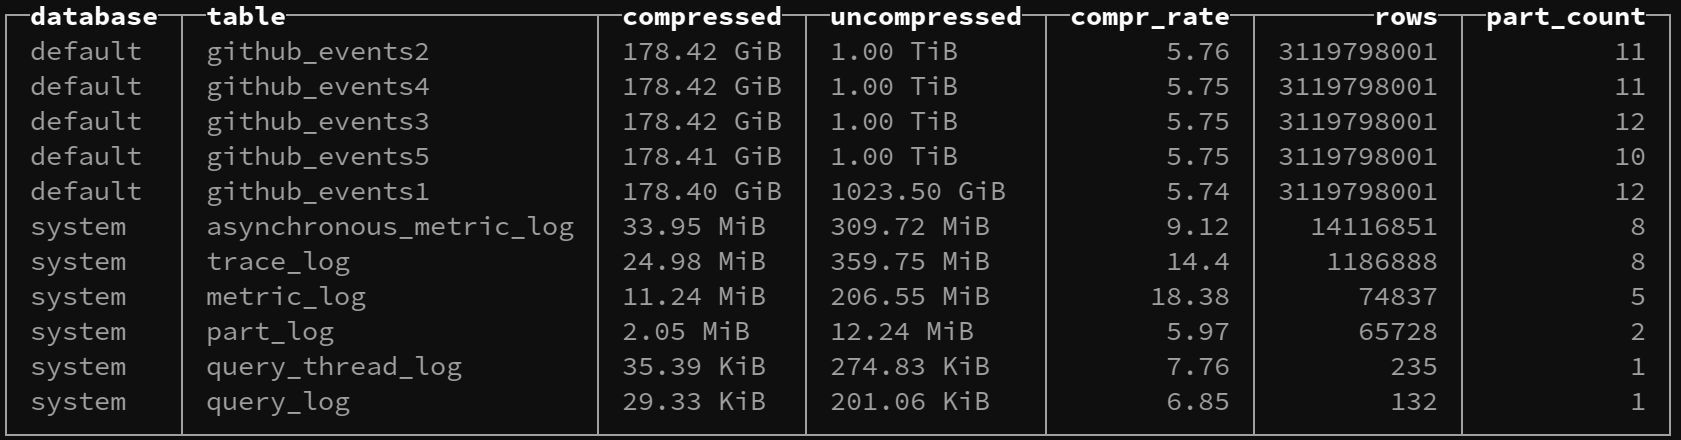
\includegraphics[width=.9\linewidth]{figures/clickhouse/table_sizes.png}
\end{center}
\subsection{Install \texttt{clickhouse-backup}}
\label{sec:org3015272}
The most recent (as of 2022-05-09) \texttt{clickhouse-backup} binary was downloaded
from \texttt{clickhouse-backup}'s GitHub page \cite{akulov_clickhouse-backup_2022}.
%[akulovClickhousebackup2022].

\begin{minted}[breaklines=true,breakanywhere=true]{bash}
# Download archive containing binary
wget https://github.com/AlexAkulov/clickhouse-backup/releases/download/v1.3.2/clickhouse-backup-linux-amd64.tar.gz

# Decompress archive
tar -zxvf clickhouse-backup-linux-amd64.tar.gz

# Move binary to home directory
mv build/linux/amd64/clickhouse-backup ~

# Cleanup
rmdir -p build/linux/amd64
rm clickhouse-backup-linux-amd64.tar.gz
\end{minted}
\subsection{Set up Azure Blob storage for use with \texttt{clickhouse-backup}}
\label{sec:orgf1120ab}
Commands run from the Azure Cloud Shell
\subsubsection{Create a storage account}
\label{sec:org7131bc2}
\begin{minted}[breaklines=true,breakanywhere=true]{powershell}
az storage account create `
    --name $SAName `
    --resource-group $RGName `
    --location eastus `
    --sku Standard_LRS `
    --encryption-services blob
\end{minted}

Output:
\begin{minted}[breaklines=true,breakanywhere=true]{json}
{
  "accessTier": "Hot",
  "allowBlobPublicAccess": true,
  "allowCrossTenantReplication": null,
  "allowSharedKeyAccess": null,
  "allowedCopyScope": null,
  "azureFilesIdentityBasedAuthentication": null,
  "blobRestoreStatus": null,
  "creationTime": "2022-05-10T09:55:00.481299+00:00",
  "customDomain": null,
  "defaultToOAuthAuthentication": null,
  "dnsEndpointType": null,
  "enableHttpsTrafficOnly": true,
  "enableNfsV3": null,
  "encryption": {
    "encryptionIdentity": null,
    "keySource": "Microsoft.Storage",
    "keyVaultProperties": null,
    "requireInfrastructureEncryption": null,
    "services": {
      "blob": {
        "enabled": true,
        "keyType": "Account",
        "lastEnabledTime": "2022-05-10T09:55:00.606291+00:00"
      },
      "file": {
        "enabled": true,
        "keyType": "Account",
        "lastEnabledTime": "2022-05-10T09:55:00.606291+00:00"
      },
      "queue": null,
      "table": null
    }
  },
  "extendedLocation": null,
  "failoverInProgress": null,
  "geoReplicationStats": null,
  "id": "/subscriptions/4b48eb85-91f3-4902-b74b-e84641fb6785/resourceGroups/perfRG/providers/Microsoft.Storage/storageAccounts/perfchbksa",
  "identity": null,
  "immutableStorageWithVersioning": null,
  "isHnsEnabled": null,
  "isLocalUserEnabled": null,
  "isSftpEnabled": null,
  "keyCreationTime": {
    "key1": "2022-05-10T09:55:00.606291+00:00",
    "key2": "2022-05-10T09:55:00.606291+00:00"
  },
  "keyPolicy": null,
  "kind": "StorageV2",
  "largeFileSharesState": null,
  "lastGeoFailoverTime": null,
  "location": "eastus",
  "minimumTlsVersion": "TLS1_0",
  "name": "perfchbksa",
  "networkRuleSet": {
    "bypass": "AzureServices",
    "defaultAction": "Allow",
    "ipRules": [],
    "resourceAccessRules": null,
    "virtualNetworkRules": []
  },
  "primaryEndpoints": {
    "blob": "https://perfchbksa.blob.core.windows.net/",
    "dfs": "https://perfchbksa.dfs.core.windows.net/",
    "file": "https://perfchbksa.file.core.windows.net/",
    "internetEndpoints": null,
    "microsoftEndpoints": null,
    "queue": "https://perfchbksa.queue.core.windows.net/",
    "table": "https://perfchbksa.table.core.windows.net/",
    "web": "https://perfchbksa.z13.web.core.windows.net/"
  },
  "primaryLocation": "eastus",
  "privateEndpointConnections": [],
  "provisioningState": "Succeeded",
  "publicNetworkAccess": null,
  "resourceGroup": "perfRG",
  "routingPreference": null,
  "sasPolicy": null,
  "secondaryEndpoints": null,
  "secondaryLocation": null,
  "sku": {
    "name": "Standard_LRS",
    "tier": "Standard"
  },
  "statusOfPrimary": "available",
  "statusOfSecondary": null,
  "storageAccountSkuConversionStatus": null,
  "tags": {},
  "type": "Microsoft.Storage/storageAccounts"
}
\end{minted}

\subsubsection{Create a storage container}
\label{sec:org80fd248}
\begin{minted}[breaklines=true,breakanywhere=true]{powershell}
az storage container create `
    --account-name $SAName `
    --name $ContainerName `
    --auth-mode login
\end{minted}

Output:
\begin{minted}[breaklines=true,breakanywhere=true]{json}
{
  "created": true
}
\end{minted}
\subsubsection{Enable soft delete for Blobs and Blob container}
\label{sec:org35b84b2}
Enable soft delete for Blob container:
\begin{minted}[breaklines=true,breakanywhere=true]{powershell}
az storage account blob-service-properties update `
    --enable-container-delete-retention true `
    --container-delete-retention-days 7 `
    --account-name $SAName `
    --resource-group $RGName
\end{minted}

Output:
\begin{minted}[breaklines=true,breakanywhere=true]{json}
{
  "automaticSnapshotPolicyEnabled": null,
  "changeFeed": null,
  "containerDeleteRetentionPolicy": {
    "allowPermanentDelete": null,
    "days": 7,
    "enabled": true
  },
  "cors": {
    "corsRules": []
  },
  "defaultServiceVersion": null,
  "deleteRetentionPolicy": {
    "allowPermanentDelete": false,
    "days": null,
    "enabled": false
  },
  "id": "/subscriptions/4b48eb85-91f3-4902-b74b-e84641fb6785/resourceGroups/perfRG/providers/Microsoft.Storage/storageAccounts/perfchbksa/blobServices/default",
  "isVersioningEnabled": null,
  "lastAccessTimeTrackingPolicy": null,
  "name": "default",
  "resourceGroup": "perfRG",
  "restorePolicy": null,
  "sku": null,
  "type": "Microsoft.Storage/storageAccounts/blobServices"
}
\end{minted}

Enable soft delete for all Blobs:
\begin{minted}[breaklines=true,breakanywhere=true]{powershell}
az storage account blob-service-properties update --account-name $SAName `
    --resource-group $RGName `
    --enable-delete-retention true `
    --delete-retention-days 7
\end{minted}

Output:
\begin{minted}[breaklines=true,breakanywhere=true]{json}
{
  "automaticSnapshotPolicyEnabled": null,
  "changeFeed": null,
  "containerDeleteRetentionPolicy": {
    "allowPermanentDelete": null,
    "days": 7,
    "enabled": true
  },
  "cors": {
    "corsRules": []
  },
  "defaultServiceVersion": null,
  "deleteRetentionPolicy": {
    "allowPermanentDelete": null,
    "days": 7,
    "enabled": true
  },
  "id": "/subscriptions/4b48eb85-91f3-4902-b74b-e84641fb6785/resourceGroups/perfRG/providers/Microsoft.Storage/storageAccounts/perfchbksa/blobServices/default",
  "isVersioningEnabled": null,
  "lastAccessTimeTrackingPolicy": null,
  "name": "default",
  "resourceGroup": "perfRG",
  "restorePolicy": null,
  "sku": null,
  "type": "Microsoft.Storage/storageAccounts/blobServices"
}
\end{minted}
\subsection{Configure \texttt{clickhouse-backup} to use Blob storage}
\label{sec:org05c9377}
\subsubsection{Get necessary config details}
\label{sec:org28a9875}
The configuration details needed to configure \texttt{clickhouse-backup} were retrieved
and copied into the configuration file.

Commands were run from the Azure Cloud Shell.

\begin{enumerate}
\item Get access key for storage account
\label{sec:org9369db9}
Get storage account keys:
\begin{minted}[breaklines=true,breakanywhere=true]{powershell}
az storage account keys list `
  --resource-group $RGName `
  --account-name $SAName
\end{minted}

Output:
\begin{minted}[breaklines=true,breakanywhere=true]{json}
[
  {
    "creationTime": "2022-05-10T09:55:00.606291+00:00",
    "keyName": "key1",
    "permissions": "FULL",
    "value": "EIhee0y3zertAVbAa7cRAhYQ/2Oui25vdr6DoL05qkA+CfZZpFMlabzJFPtJG8Xdc735PAbA8w8r+AStl89ieA=="
  },
  {
    "creationTime": "2022-05-10T09:55:00.606291+00:00",
    "keyName": "key2",
    "permissions": "FULL",
    "value": "4Rm6943iYttVqjLBE/csYCa7rnS02xQKjAPW7C/sScZ189My20+/Opl0HmOql1CLnL53x5NYzB/5+AStAqv2kw=="
  }
]
\end{minted}

\texttt{key1} was copied.

\item Get SAS token for container
\label{sec:org2a7114d}
Generate SAS token
\begin{minted}[breaklines=true,breakanywhere=true]{powershell}
az storage container generate-sas `
    --account-name $SAName `
    --name $ContainerName `
    --permissions acdlrw `
    --expiry $SASExpDate `
    --auth-mode login `
    --as-user
\end{minted}

Output:

\begin{minted}[breaklines=true,breakanywhere=true]{text}
"se=2022-05-18&sp=racwdl&sv=2021-04-10&sr=c&skoid=d404139d-e156-421c-9450-19e9734a8141&sktid=09a10672-822f-4467-a5ba-5bb375967c05&skt=2022-05-11T07%3A01%3A18Z&ske=2022-05-18T00%3A00%3A00Z&sks=b&skv=2021-04-10&sig=GgFsZifUWr0r71gCZaD9PbxRXrybhWS09Hpb2scfsKg%3D"
\end{minted}
\end{enumerate}
\subsubsection{Configure \texttt{clickhouse-backup} to use Blob storage}
\label{sec:org265a2b6}
The configuration file from the non-performance test environment
was copied and modified to use the new account key and SAS token.
\texttt{account\_name}, \texttt{container} and \texttt{path} was also modified.
It was saved as \path{/home/azureuser/config.yaml} on the ClickHouse VM.

\begin{minted}[breaklines=true,breakanywhere=true]{yaml}
general:
  remote_storage: azblob
  max_file_size: 0
  disable_progress_bar: false
  backups_to_keep_local: 0
  backups_to_keep_remote: 0
  log_level: info
  allow_empty_backups: false
  download_concurrency: 1
  upload_concurrency: 1
  restore_schema_on_cluster: ""
  upload_by_part: true
  download_by_part: true
clickhouse:
  username: default
  password: ""
  host: localhost
  port: 9000
  disk_mapping: {}
  skip_tables:
  - system.*
  - INFORMATION_SCHEMA.*
  - information_schema.*
  timeout: 5m
  freeze_by_part: false
  secure: false
  skip_verify: false
  sync_replicated_tables: false
  log_sql_queries: true
  config_dir: /etc/clickhouse-server/
  restart_command: systemctl restart clickhouse-server
  ignore_not_exists_error_during_freeze: true
  tls_key: ""
  tls_cert: ""
  tls_ca: ""
  debug: false
s3:
  access_key: ""
  secret_key: ""
  bucket: ""
  endpoint: ""
  region: us-east-1
  acl: private
  assume_role_arn: ""
  force_path_style: false
  path: ""
  disable_ssl: false
  compression_level: 1
  compression_format: tar
  sse: ""
  disable_cert_verification: false
  storage_class: STANDARD
  concurrency: 1
  part_size: 0
  max_parts_count: 10000
  debug: false
gcs:
  credentials_file: ""
  credentials_json: ""
  bucket: ""
  path: ""
  compression_level: 1
  compression_format: tar
  debug: false
  endpoint: ""
cos:
  url: ""
  timeout: 2m
  secret_id: ""
  secret_key: ""
  path: ""
  compression_format: tar
  compression_level: 1
  debug: false
api:
  listen: localhost:7171
  enable_metrics: true
  enable_pprof: false
  username: ""
  password: ""
  secure: false
  certificate_file: ""
  private_key_file: ""
  create_integration_tables: false
  allow_parallel: false
ftp:
  address: ""
  timeout: 2m
  username: ""
  password: ""
  tls: false
  path: ""
  compression_format: tar
  compression_level: 1
  concurrency: 1
  debug: false
sftp:
  address: ""
  port: 22
  username: ""
  password: ""
  key: ""
  path: ""
  compression_format: tar
  compression_level: 1
  concurrency: 1
  debug: false
azblob:
  endpoint_suffix: core.windows.net
  account_name: "perfchbksa"
  account_key: "EIhee0y3zertAVbAa7cRAhYQ/2Oui25vdr6DoL05qkA+CfZZpFMlabzJFPtJG8Xdc735PAbA8w8r+AStl89ieA=="
  sas: "se=2022-05-18&sp=racwdl&sv=2021-04-10&sr=c&skoid=d404139d-e156-421c-9450-19e9734a8141&sktid=09a10672-822f-4467-a5ba-5bb375967c05&skt=2022-05-11T07%3A01%3A18Z&ske=2022-05-18T00%3A00%3A00Z&sks=b&skv=2021-04-10&sig=GgFsZifUWr0r71gCZaD9PbxRXrybhWS09Hpb2scfsKg%3D"
  use_managed_identity: false
  container: "chbkperfcontainer"
  path: "https://perfchbksa.blob.core.windows.net/chbkperfcontainer"
  compression_level: 1
  compression_format: tar
  sse_key: ""
  buffer_size: 0
  buffer_count: 3
  max_parts_count: 1
\end{minted}

\subsubsection{Perform remote backup}
\label{sec:org982a0d7}
Commands were run in \texttt{bash} on the ClickHouse VM.

While the time to \emph{make} backups was not one of the criteria
we decided to focus on, we measured the time anyway.
The time was measured using the builtin bash tool \texttt{time}.
In order to avoid timing \texttt{sudo} the commands were run as \texttt{root}.

Create a remote backup:
\begin{minted}[breaklines=true,breakanywhere=true]{bash}
time ./clickhouse-backup create_remote --config config.yaml
\end{minted}

Time to make a full backup with \texttt{clickhouse-backup}:
\begin{minted}[breaklines=true,breakanywhere=true]{text}
real    198m48.369s
user    14m17.555s
sys     12m38.432s
\end{minted}

List remote backups:
\begin{minted}[breaklines=true,breakanywhere=true]{bash}
./clickhouse-backup list remote --config config.yaml
# 2022/05/11 10:59:53.978855  info SELECT max(toInt64(bytes_on_disk * 1.02)) AS max_file_size FROM system.parts
# 2022-05-11T07-25-16   895.29GiB   11/05/2022 10:44:05   remote      tar
\end{minted}

895GiB is roughly equal to 961GB, which seems correct based on the table sizes.

\subsection{Set up Azure Backup}
\label{sec:org29e551a}
\subsubsection{Create a Recovery Services vault}
\label{sec:orgc6db81c}
\begin{minted}[breaklines=true,breakanywhere=true]{powershell}
az backup vault create --location $location --name $RSVName --resource-group $RGName
\end{minted}

Output:
\begin{minted}[breaklines=true,breakanywhere=true]{json}
{
  "etag": "W/\"datetime'2022-05-10T09%3A58%3A14.2637541Z'\"",
  "id": "/subscriptions/4b48eb85-91f3-4902-b74b-e84641fb6785/resourceGroups/perfRG/providers/Microsoft.RecoveryServices/vaults/perfRSV",
  "identity": null,
  "location": "eastus",
  "name": "perfRSV",
  "properties": {
    "encryption": null,
    "privateEndpointConnections": null,
    "privateEndpointStateForBackup": "None",
    "privateEndpointStateForSiteRecovery": "None",
    "provisioningState": "Succeeded",
    "upgradeDetails": null
  },
  "resourceGroup": "perfRG",
  "sku": {
    "name": "Standard",
    "tier": null
  },
  "systemData": null,
  "tags": null,
  "type": "Microsoft.RecoveryServices/vaults"
}
\end{minted}

\subsubsection{Disable geo-redundancy}
\label{sec:org5e6a978}
\begin{minted}[breaklines=true,breakanywhere=true]{powershell}
az backup vault backup-properties set --backup-storage-redundancy LocallyRedundant --name $RSVName --resource-group $RGName --subscription $subscription
\end{minted}

Output:
\begin{minted}[breaklines=true,breakanywhere=true]{json}
{
  "eTag": null,
  "id": "/subscriptions/4b48eb85-91f3-4902-b74b-e84641fb6785/resourceGroups/perfRG/providers/Microsoft.RecoveryServices/vaults/perfRSV/backupstorageconfig/vaultstorageconfig",
  "location": null,
  "name": "vaultstorageconfig",
  "properties": {
    "crossRegionRestoreFlag": false,
    "dedupState": "Disabled",
    "storageModelType": "LocallyRedundant",
    "storageType": "LocallyRedundant",
    "storageTypeState": "Unlocked",
    "xcoolState": "Disabled"
  },
  "resourceGroup": "perfRG",
  "tags": null,
  "type": "Microsoft.RecoveryServices/vaults/backupstorageconfig"
}
\end{minted}
\subsubsection{Enable backup for the VM}
\label{sec:org6d56370}
\begin{minted}[breaklines=true,breakanywhere=true]{powershell}
az backup protection enable-for-vm `
 --resource-group $RGName `
 --vault-name $RSVName `
 --vm $CHName `
 --policy-name $PolicyName
\end{minted}

Output:
\begin{minted}[breaklines=true,breakanywhere=true]{json}
{
  "eTag": null,
  "id": "/subscriptions/4b48eb85-91f3-4902-b74b-e84641fb6785/resourceGroups/perfRG/providers/Microsoft.RecoveryServices/vaults/perfRSV/backupJobs/e17cce76-2b1e-47e4-a47d-07672d5400cc",
  "location": null,
  "name": "e17cce76-2b1e-47e4-a47d-07672d5400cc",
  "properties": {
    "actionsInfo": null,
    "activityId": "529e46da-d11a-11ec-aebb-0a580af40666",
    "backupManagementType": "AzureIaasVM",
    "containerName": "iaasvmcontainerv2;perfrg;perfclickhousevm",
    "duration": "0:00:30.947098",
    "endTime": "2022-05-11T11:06:30.280573+00:00",
    "entityFriendlyName": "perfclickhousevm",
    "errorDetails": null,
    "extendedInfo": {
      "dynamicErrorMessage": null,
      "estimatedRemainingDuration": null,
      "internalPropertyBag": null,
      "progressPercentage": null,
      "propertyBag": {
        "Policy Name": "DefaultPolicy",
        "VM Name": "perfclickhousevm"
      },
      "tasksList": []
    },
    "isUserTriggered": null,
    "jobType": "AzureIaaSVMJob",
    "operation": "ConfigureBackup",
    "startTime": "2022-05-11T11:05:59.333474+00:00",
    "status": "Completed",
    "virtualMachineVersion": "Compute"
  },
  "resourceGroup": "perfRG",
  "tags": null,
  "type": "Microsoft.RecoveryServices/vaults/backupJobs"
}
\end{minted}

\subsubsection{Make a backup of the ClickHouse VM}
\label{sec:org448ef16}
Instantly trigger a backup job:
\begin{minted}[breaklines=true,breakanywhere=true]{powershell}
az backup protection backup-now `
    --resource-group $RGName `
    --vault-name $RSVName `
    --container-name $CHName `
    --item-name $CHName `
    --backup-management-type AzureIaaSVM `
    --retain-until 18-05-2022
\end{minted}

Output:
\begin{minted}[breaklines=true,breakanywhere=true]{json}
{
  "eTag": null,
  "id": "/subscriptions/4b48eb85-91f3-4902-b74b-e84641fb6785/resourceGroups/perfRG/providers/Microsoft.RecoveryServices/vaults/perfRSV/backupJobs/07a1a270-885a-4210-b7bf-c51f2dcacdad",
  "location": null,
  "name": "07a1a270-885a-4210-b7bf-c51f2dcacdad",
  "properties": {
    "actionsInfo": [
      "1"
    ],
    "activityId": "bb5f9db8-d11a-11ec-8215-0a580af40666",
    "backupManagementType": "AzureIaasVM",
    "containerName": "iaasvmcontainerv2;perfrg;perfclickhousevm",
    "duration": "0:00:01.278993",
    "endTime": null,
    "entityFriendlyName": "perfclickhousevm",
    "errorDetails": null,
    "extendedInfo": {
      "dynamicErrorMessage": null,
      "estimatedRemainingDuration": null,
      "internalPropertyBag": {
        "IsInstantRpJob": "True"
      },
      "progressPercentage": null,
      "propertyBag": {
        "Recovery Point Expiry Time in UTC": "5/18/2022 12:00:00 AM",
        "VM Name": "perfclickhousevm"
      },
      "tasksList": [
        {
          "duration": "0:00:00",
          "endTime": null,
          "instanceId": null,
          "progressPercentage": null,
          "startTime": null,
          "status": "InProgress",
          "taskExecutionDetails": null,
          "taskId": "Take Snapshot"
        },
        {
          "duration": "0:00:00",
          "endTime": null,
          "instanceId": null,
          "progressPercentage": null,
          "startTime": null,
          "status": "NotStarted",
          "taskExecutionDetails": null,
          "taskId": "Transfer data to vault"
        }
      ]
    },
    "isUserTriggered": null,
    "jobType": "AzureIaaSVMJob",
    "operation": "Backup",
    "startTime": "2022-05-11T11:08:52.010975+00:00",
    "status": "InProgress",
    "virtualMachineVersion": "Compute"
  },
  "resourceGroup": "perfRG",
  "tags": null,
  "type": "Microsoft.RecoveryServices/vaults/backupJobs"
}
\end{minted}
\subsubsection{Create a storage account for staging}
\label{sec:orgdb0da58}
A storage account is needed to stage recoveries from Azure Backup.

Create storage account:
\begin{minted}[breaklines=true,breakanywhere=true]{powershell}
az storage account create `
    --name $StagingSAName `
    --resource-group $RGName `
    --location eastus `
    --sku Standard_LRS
\end{minted}

\begin{minted}[breaklines=true,breakanywhere=true]{json}
{
  "accessTier": "Hot",
  "allowBlobPublicAccess": true,
  "allowCrossTenantReplication": null,
  "allowSharedKeyAccess": null,
  "allowedCopyScope": null,
  "azureFilesIdentityBasedAuthentication": null,
  "blobRestoreStatus": null,
  "creationTime": "2022-05-12T06:35:41.131490+00:00",
  "customDomain": null,
  "defaultToOAuthAuthentication": null,
  "dnsEndpointType": null,
  "enableHttpsTrafficOnly": true,
  "enableNfsV3": null,
  "encryption": {
    "encryptionIdentity": null,
    "keySource": "Microsoft.Storage",
    "keyVaultProperties": null,
    "requireInfrastructureEncryption": null,
    "services": {
      "blob": {
        "enabled": true,
        "keyType": "Account",
        "lastEnabledTime": "2022-05-12T06:35:41.272095+00:00"
      },
      "file": {
        "enabled": true,
        "keyType": "Account",
        "lastEnabledTime": "2022-05-12T06:35:41.272095+00:00"
      },
      "queue": null,
      "table": null
    }
  },
  "extendedLocation": null,
  "failoverInProgress": null,
  "geoReplicationStats": null,
  "id": "/subscriptions/4b48eb85-91f3-4902-b74b-e84641fb6785/resourceGroups/perfRG/providers/Microsoft.Storage/storageAccounts/perfstagingchsa",
  "identity": null,
  "immutableStorageWithVersioning": null,
  "isHnsEnabled": null,
  "isLocalUserEnabled": null,
  "isSftpEnabled": null,
  "keyCreationTime": {
    "key1": "2022-05-12T06:35:41.256500+00:00",
    "key2": "2022-05-12T06:35:41.256500+00:00"
  },
  "keyPolicy": null,
  "kind": "StorageV2",
  "largeFileSharesState": null,
  "lastGeoFailoverTime": null,
  "location": "eastus",
  "minimumTlsVersion": "TLS1_0",
  "name": "perfstagingchsa",
  "networkRuleSet": {
    "bypass": "AzureServices",
    "defaultAction": "Allow",
    "ipRules": [],
    "resourceAccessRules": null,
    "virtualNetworkRules": []
  },
  "primaryEndpoints": {
    "blob": "https://perfstagingchsa.blob.core.windows.net/",
    "dfs": "https://perfstagingchsa.dfs.core.windows.net/",
    "file": "https://perfstagingchsa.file.core.windows.net/",
    "internetEndpoints": null,
    "microsoftEndpoints": null,
    "queue": "https://perfstagingchsa.queue.core.windows.net/",
    "table": "https://perfstagingchsa.table.core.windows.net/",
    "web": "https://perfstagingchsa.z13.web.core.windows.net/"
  },
  "primaryLocation": "eastus",
  "privateEndpointConnections": [],
  "provisioningState": "Succeeded",
  "publicNetworkAccess": null,
  "resourceGroup": "perfRG",
  "routingPreference": null,
  "sasPolicy": null,
  "secondaryEndpoints": null,
  "secondaryLocation": null,
  "sku": {
    "name": "Standard_LRS",
    "tier": "Standard"
  },
  "statusOfPrimary": "available",
  "statusOfSecondary": null,
  "storageAccountSkuConversionStatus": null,
  "tags": {},
  "type": "Microsoft.Storage/storageAccounts"
}
\end{minted}

 \section{Azure Backup performance tests}
\label{app:chab-perf}
Four attempts were made at recovering the VM with Azure Backup.
The first two failed, presumably because something was wrong with the restore point used.

The two last attempts used a different restore point.
The time spent was measured using a stopwatch.
Measurements were started the moment the restore job was started
and stopped when it was possible to SSH to the VM and query the database.

Azure measures the time taken by the restore job itself.
This is noted separately.
The total time is influenced by how fast we were able to paste commands into the CLI.
The restore job time is probably the most interesting time.

Recovery using Azure Portal:
\begin{center}
\begin{tabular}{lr}
\hline
 & Time (hours:minutes:seconds)\\
\hline
Restore job: & 00:02:10\\
Total: & 00:03:30\\
\hline
\end{tabular}
\end{center}

Recovery using Azure CLI:
\begin{center}
\begin{tabular}{lr}
\hline
 & Time (hours:minutes:seconds)\\
\hline
Restore job: & 00:01:06\\
Total: & 00:06:33\\
\hline
\end{tabular}
\end{center}


\subsection{Recovery with Azure Backup via CLI (failed first attempt)}
\label{sec:orgb039355}
\subsubsection{Delete VM}
\label{sec:org5859260}
There are not enough vCPUs available in the quota,
which means the VM has to be deleted before recovery can happen.

\begin{minted}[breaklines=true,breakanywhere=true]{powershell}
az vm delete --name $CHName --resource-group $RGName --yes
\end{minted}

\subsubsection{Preparation}
\label{sec:orgd393ff5}
Prepare environment and retrieve restore points
\begin{minted}[breaklines=true,breakanywhere=true]{powershell}
# Get RSV and set context
$RSV = Get-AzRecoveryServicesVault -Name $RSVName -ResourceGroupName $RGName
Set-AzRecoveryServicesVaultContext -Vault $RSV

# Select VM
$namedContainer = Get-AzRecoveryServicesBackupContainer  -ContainerType "AzureVM" -Status "Registered" -FriendlyName $CHName -VaultId $RSV.ID
$backupitem = Get-AzRecoveryServicesBackupItem -Container $namedContainer  -WorkloadType "AzureVM" -VaultId $RSV.ID

# Get start and end date
$startDate = (Get-Date).AddDays(-7)
$endDate = Get-Date

# Store recovery points in variable
$rp = Get-AzRecoveryServicesBackupRecoveryPoint -Item $backupitem -StartDate $startdate.ToUniversalTime() -EndDate $enddate.ToUniversalTime() -VaultId $RSV.ID
\end{minted}

List contents of \texttt{\$rp}:
\begin{minted}[breaklines=true,breakanywhere=true]{powershell}
$rp
# RecoveryPointId    RecoveryPointType  RecoveryPointTime      ContainerName                        ContainerType
# ---------------    -----------------  -----------------      -------------                        -------------
# 15649757922643     FileSystemConsist… 5/11/2022 7:44:53 PM   iaasvmcontainerv2;perfrg;perfclickh… AzureVM
# 12290901249728     FileSystemConsist… 5/11/2022 11:09:00 AM  iaasvmcontainerv2;perfrg;perfclickh… AzureVM
\end{minted}

12290901249728 is the point that was triggered manually when Azure Backup was set up (see \ref{app:ch-perf}).
The point is stored in \texttt{\$rp[1]}.

\subsubsection{Create restore job}
\label{sec:orgd99419b}
Start restore job:
\begin{minted}[breaklines=true,breakanywhere=true]{powershell}
# Select recovery point
$RecPoint = $rp[1]

# Create a restore job for the backup item
$restorejob = Restore-AzRecoveryServicesBackupItem -RecoveryPoint $RecPoint -StorageAccountName $StagingSAName -StorageAccountResourceGroupName $RGName -TargetResourceGroupName $RGName -VaultId $RSV.ID

# Wait for the restore job to complete
Wait-AzRecoveryServicesBackupJob -Job $restorejob -Timeout 43200
# WorkloadName     Operation            Status               StartTime                 EndTime                   JobID
# ------------     ---------            ------               ---------                 -------                   -----
# perfclickhousevm Restore              Completed            5/12/2022 7:13:45 AM      5/12/2022 7:14:51 AM      30d32412-e718-4dde-a52e-c48444364cf3

# Get details of the restore job
$restorejob = Get-AzRecoveryServicesBackupJob -Job $restorejob -VaultId $RSV.ID
$details = Get-AzRecoveryServicesBackupJobDetail -Job $restorejob -VaultId $RSV.ID
\end{minted}

Contents of \texttt{\$details.Properties}:
\begin{minted}[breaklines=true,breakanywhere=true]{powershell}
$details.Properties

# Key                         Value
# ---                         -----
# Job Type                    Recover disks
# Target VM Name              vmName
# Target Storage Account Name perfstagingchsa
# Recovery point time         5/11/2022 11:09:00 AM
# Config Blob Name            config-perfclickhousevm-30d32412-e718-4dde-a52e-c48444364cf3.json
# Config Blob Container Name  perfclickhousevm-8726c9fbe67e4ca4a5ff7e06238eac29
# Config Blob Uri             https://perfstagingchsa.blob.core.windows.net/perfclickhousevm-8726c9fbe67e4ca4a5ff7e06238eac29/config-perfclickhousevm-30d32412-e718-4dde-a52e-c48444364cf3.json
# Target resource group       perfRG
# Template Blob Uri           https://perfstagingchsa.blob.core.windows.net/perfclickhousevm-8726c9fbe67e4ca4a5ff7e06238eac29/azuredeploy30d32412-e718-4dde-a52e-c48444364cf3.json
\end{minted}

Save details:
\begin{minted}[breaklines=true,breakanywhere=true]{powershell}
$properties = $details.properties
$storageAccountName = $properties["Target Storage Account Name"]
$containerName = $properties["Config Blob Container Name"]
$templateBlobURI = $properties["Template Blob Uri"]
\end{minted}

\subsubsection{Deploy VM}
\label{sec:orgd09ce0a}
Deploy VM:
\begin{minted}[breaklines=true,breakanywhere=true]{powershell}
# Template name was copied from the last part of "Template Blob Uri"
$templateName = "azuredeploy30d32412-e718-4dde-a52e-c48444364cf3.json"

# Set the storage account
Set-AzCurrentStorageAccount -Name $storageAccountName -ResourceGroupName $RGName

# Generate SAS token
$templateBlobFullURI = New-AzStorageBlobSASToken -Container $containerName -Blob $templateName -Permission r -FullUri

# Deploy VM (VirtualMachineName had to be specified interactively)
New-AzResourceGroupDeployment -Name $CHName -ResourceGroupName $RGName -TemplateUri $templateBlobFullURI
#DeploymentName          : perfClickhouseVM
#ResourceGroupName       : perfRG
#ProvisioningState       : Succeeded
#Timestamp               : 5/12/2022 7:20:25 AM
#Mode                    : Incremental
#TemplateLink            :
#         Uri            : https://perfstagingchsa.blob.core.windows.net/perfclickhousevm-8726c9fbe67e4ca4a5ff7e06238eac29/azuredeploy30d32412-e718-4dde-a52e-c48444364cf3.json?sv=2021-04-10&se=2022-05-12T08%3A19%3A11Z&sr=b&sp=r
#         &sig=5Uzo66b%2B1I9IvrpVokKaqHtJiBCx0ZEl6r8SIyM0XGc%3D
#         ContentVersion : 1.0.0.0
#
#Parameters              :
# Name                           Type                       Value
# =============================  =========================  ==========
# virtualMachineName             String                     "perfClickhouseVM"
# virtualNetwork                 String                     "perfClickhouseVMVNET"
# virtualNetworkResourceGroup    String                     "perfRG"
# subnet                         String                     "perfClickhouseVMSubnet"
# osDiskName                     String                     "perfClickhouseVMOSDisk"
# networkInterfacePrefixName     String                     "perfClickhouseVMRestoredNIC"
# publicIpAddressName            String                     "perfClickhouseVMRestoredip"
#
#Outputs                 :
#DeploymentDebugLogLevel :
\end{minted}

\subsubsection{Trouble connecting to the VM}
\label{sec:org3c86200}
\texttt{clickhouse-client} would not start at first.
The VM was therefore restarted.
After this, SSH would time out repeatedly.
The VM was restarted again, but SSH still did not work.
Azure's SSH ``Connection troubleshoot'' in the Azure Portal was attempted,
but it would also hang for a long time.

Another attempt at recovering the data was attempted with the Azure Portal.
The recovery appears to have succeeded.
The same problems with \texttt{clickhouse-client} not starting,
and SSH timing out still appeared, though.
Maybe the restore point was broken in some way.

We decided to abort the attempt at recovering with Azure Backup for now.
Instead, we decided to try to recover with \texttt{clickhouse-backup} instead,
and then make a new restore point in Azure Backup to recover from.

\subsection{Recovery with Azure Backup (failed second attempt)}
\label{sec:org2c0f303}
We tried to recover from Azure Backup once again.
Output was omitted for brevity, except for when waiting for the restore job,
as that output contains information about the time the restore job took.

\subsubsection{Delete VM}
\label{sec:org0fbc45f}
\begin{minted}[breaklines=true,breakanywhere=true]{powershell}
az vm delete --name $CHName --resource-group $RGName --yes
\end{minted}

\subsubsection{Get restore point}
\label{sec:orgd8ba7ae}
\begin{minted}[breaklines=true,breakanywhere=true]{powershell}
# Get RSV and set context
$RSV = Get-AzRecoveryServicesVault -Name $RSVName -ResourceGroupName $RGName
Set-AzRecoveryServicesVaultContext -Vault $RSV

# Select VM
$namedContainer = Get-AzRecoveryServicesBackupContainer  -ContainerType "AzureVM" -Status "Registered" -FriendlyName $CHName -VaultId $RSV.ID
$backupitem = Get-AzRecoveryServicesBackupItem -Container $namedContainer  -WorkloadType "AzureVM" -VaultId $RSV.ID

# Get start and end date
$startDate = (Get-Date).AddDays(-7)
$endDate = Get-Date

# Store recovery points in variable
$rp = Get-AzRecoveryServicesBackupRecoveryPoint -Item $backupitem -StartDate $startdate.ToUniversalTime() -EndDate $enddate.ToUniversalTime() -VaultId $RSV.ID
\end{minted}

\subsubsection{Restore}
\label{sec:org22dad73}
Start restore job:
\begin{minted}[breaklines=true,breakanywhere=true]{powershell}
# Select recovery point
$RecPoint = $rp[1]

# Create a restore job for the backup item
$restorejob = Restore-AzRecoveryServicesBackupItem -RecoveryPoint $RecPoint -StorageAccountName $StagingSAName -StorageAccountResourceGroupName $RGName -TargetResourceGroupName $RGName -VaultId $RSV.ID

# Wait for the restore job to complete
Wait-AzRecoveryServicesBackupJob -Job $restorejob -Timeout 43200
# WorkloadName     Operation            Status               StartTime                 EndTime                   JobID
# ------------     ---------            ------               ---------                 -------                   -----
# perfclickhousevm Restore              Completed            5/12/2022 11:30:24 AM     5/12/2022 11:31:34 AM     2940f1d3-b57f-4428-9b1b-066e116a1389

# Get details of the restore job
$restorejob = Get-AzRecoveryServicesBackupJob -Job $restorejob -VaultId $RSV.ID
$details = Get-AzRecoveryServicesBackupJobDetail -Job $restorejob -VaultId $RSV.ID
\end{minted}

Save details:
\begin{minted}[breaklines=true,breakanywhere=true]{powershell}
$properties = $details.properties
$storageAccountName = $properties["Target Storage Account Name"]
$containerName = $properties["Config Blob Container Name"]
$templateBlobURI = $properties["Template Blob Uri"]
\end{minted}

\subsubsection{Deploy VM (failed)}
\label{sec:org9eacaf3}
Deploy VM:
\begin{minted}[breaklines=true,breakanywhere=true]{powershell}
# Template name was copied from the last part of "Template Blob Uri"
$templateName = "azuredeploy2940f1d3-b57f-4428-9b1b-066e116a1389.json"

# Set the storage account
Set-AzCurrentStorageAccount -Name $storageAccountName -ResourceGroupName $RGName

# Generate SAS token
$templateBlobFullURI = New-AzStorageBlobSASToken -Container $containerName -Blob $templateName -Permission r -FullUri

# Deploy VM (VirtualMachineName had to be specified interactively)
New-AzResourceGroupDeployment -Name $CHName -ResourceGroupName $RGName -TemplateUri $templateBlobFullURI
# New-AzResourceGroupDeployment: 11:34:35 AM - The deployment 'perfClickhouseVM' failed with error(s). Showing 1 out of 1 error(s).
# Status Message: Resource /subscriptions/4b48eb85-91f3-4902-b74b-e84641fb6785/resourceGroups/perfRG/providers/Microsoft.Network/networkInterfaces/perfClickhouseVMRestoredNIC5324890b7fe44a77ae9def7a461b6e81/ipConfigurations/c0dbf1d5514749ec849957897d9405d1 is referencing public IP address /subscriptions/4b48eb85-91f3-4902-b74b-e84641fb6785/resourceGroups/perfRG/providers/Microsoft.Network/publicIPAddresses/perfClickhouseVMRestoredip that is already allocated to resource /subscriptions/4b48eb85-91f3-4902-b74b-e84641fb6785/resourceGroups/perfRG/providers/Microsoft.Network/networkInterfaces/perfClickhouseVMRestoredNICb9bd95260138425bab106f324a42acbc/ipConfigurations/7ba12bb4efcf444d9f08dd1aff9a1cc6. (Code: PublicIPAddressInUse)
# CorrelationId: 2677f822-ff57-4405-8600-c96b2eb802b4
#
# DeploymentName          : perfClickhouseVM
# ResourceGroupName       : perfRG
# ProvisioningState       : Failed
# Timestamp               : 5/12/2022 11:34:30 AM
# Mode                    : Incremental
# TemplateLink            :
#                           Uri            : https://perfstagingchsa.blob.core.windows.net/perfclickhousevm-b52ea1d968e04fc68ea92dea4d441451/azuredeploy2940f1d3-b57f-4428-9b1b-066e116a1389.json?sv=2
#                           021-04-10&se=2022-05-12T12%3A33%3A08Z&sr=b&sp=r&sig=ELTwTiFCjOc3kLiTipWd0cElPgJcGFidk8EXxJxaYfU%3D
#                           ContentVersion : 1.0.0.0
#
# Parameters              :
#                           Name                           Type                       Value
#                           =============================  =========================  ==========
#                           virtualMachineName             String                     "perfClickhouseVM"
#                           virtualNetwork                 String                     "perfClickhouseVMVNET"
#                           virtualNetworkResourceGroup    String                     "perfRG"
#                           subnet                         String                     "perfClickhouseVMSubnet"
#                           osDiskName                     String                     "perfClickhouseVMOSDisk"
#                           networkInterfacePrefixName     String                     "perfClickhouseVMRestoredNIC"
#                           publicIpAddressName            String                     "perfClickhouseVMRestoredip"
#
# Outputs                 :
\end{minted}

The deployment failed because the IP address was consider to already be in use.
The Azure Portal seems to be able to deal with these kinds of conflicts better,
so we tried to deploy using the Portal.

\subsubsection{Deploy VM using the Azure Portal}
\label{sec:org9b58952}
We decided to try to restore the VM using the Azure Portal,
instead of the CLI.

Restoring the VM using the Azure Portal:
\begin{center}
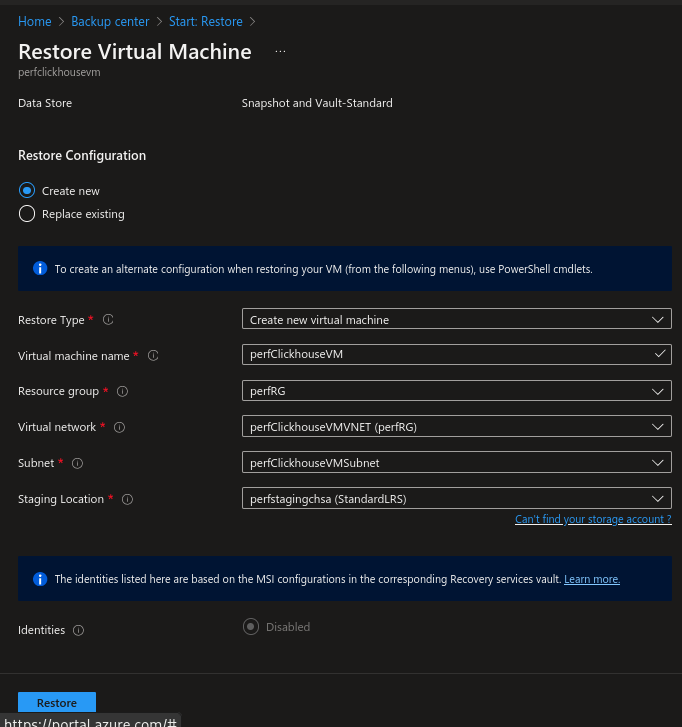
\includegraphics[width=.9\linewidth]{figures/clickhouse/azure_restore_portal.png}
\end{center}

According to the Azure Portal, the duration of the restore
was 2 minutes and 15 seconds.

Details for the restore job:
\begin{center}
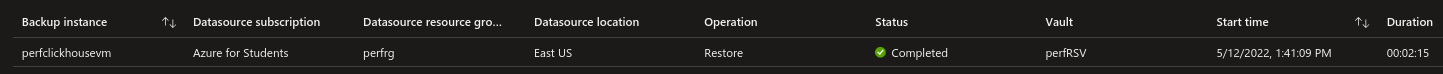
\includegraphics[width=.9\linewidth]{figures/clickhouse/ab_restore_duration.png}
\end{center}

\subsubsection{Connect to VM and verify recovery}
\label{sec:org7097732}
At first \texttt{clickhouse-client} would not start.
Several attempt were made at starting or restarting the ClickHouse server with
\texttt{sudo systemctl [start/restart] clickhouse-server.service}.

We attempted to reboot the VM.
After that, we experienced the same problem as earlier, where SSH would not connect.

After a lot of troubleshooting, we gave up.

\subsection{Recovery with Azure Backup via Portal (successful third attempt)}
\label{sec:org1aa719c}
The VM was first deleted using the Azure Portal.

The VM was then restored from a different restore point
(one that was automatically created on the same day, but later).

Restoring the VM:
\begin{center}
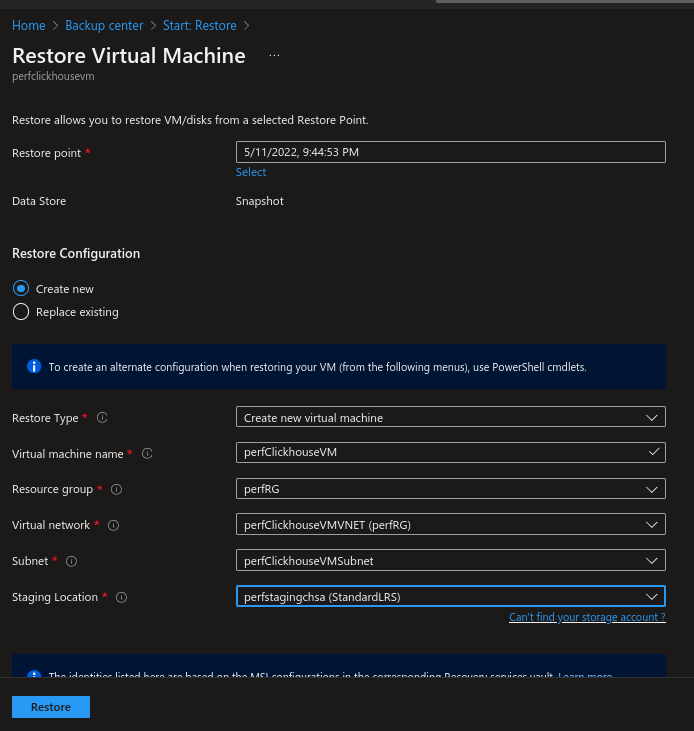
\includegraphics[width=.9\linewidth]{figures/clickhouse/ab_restore_2.png}
\end{center}

The duration was 2 minutes, 10 seconds:
\begin{center}
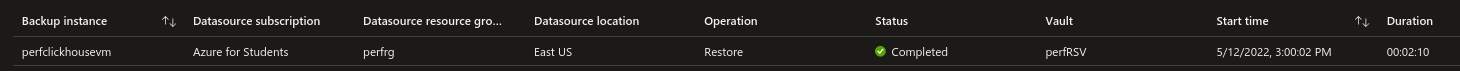
\includegraphics[width=.9\linewidth]{figures/clickhouse/ab_restore2_duration.png}
\end{center}

We were able to connect to the VM immediately.
\texttt{clickhouse-client} would not start on the first boot.
The server was rebooted.
After this, \texttt{clickhouse-client} started like normal.
It took 1 minutes and 20 seconds to get \texttt{clickhouse-client} up and running after the restore job.
The total time for the entire restoration was 3 minutes and 30 seconds.

Listing the table sizes:
\begin{minted}[breaklines=true,breakanywhere=true]{sql}
SELECT
    database,
    table,
    formatReadableSize(sum(data_compressed_bytes) AS size) AS compressed,
    formatReadableSize(sum(data_uncompressed_bytes) AS usize) AS uncompressed,
    round(usize / size, 2) AS compr_rate,
    sum(rows) AS rows,
    count() AS part_count
FROM system.parts
WHERE (active = 1) AND (database LIKE '%') AND (table LIKE '%')
GROUP BY
    database,
    table
ORDER BY size DESC
\end{minted}

Result:
\begin{center}
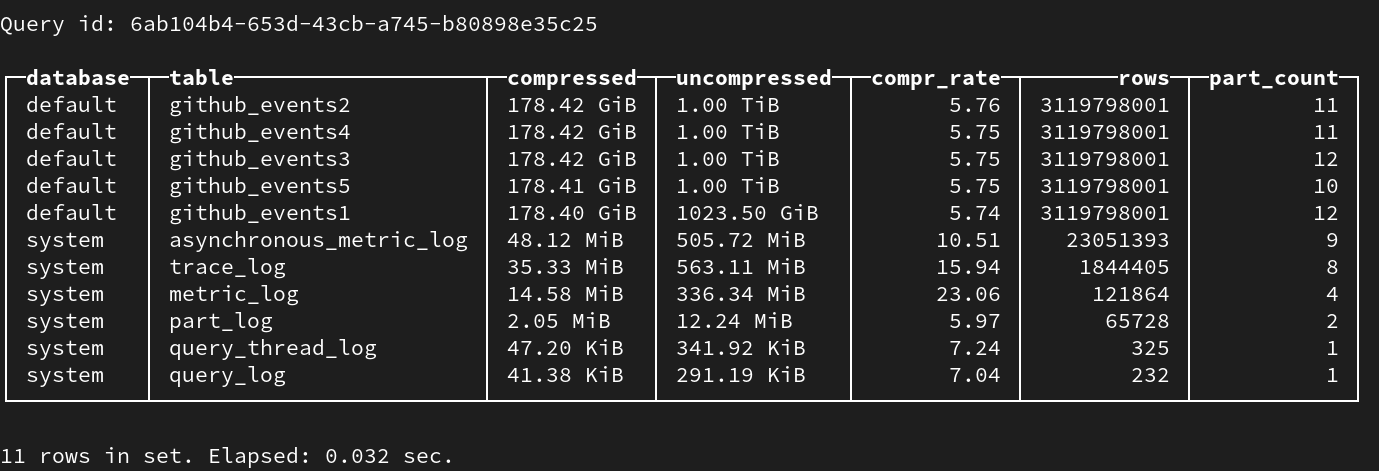
\includegraphics[width=.9\linewidth]{figures/clickhouse/ab_restore2_tables.png}
\end{center}

Everything appears to be in order.

\subsection{Recovery with Azure Backup via CLI (successful fourth attempt)}
\label{sec:orgcd90f70}
We decided to try to recover the VM via the CLI one last time,
this time using the same restore point as we did in the successful
attempt where we used the Azure Portal.

The restore job itself took 1 minute and 6 seconds.
The total time was 6 minutes and 33 seconds.

\subsubsection{Preparation}
\label{sec:org012927e}
Delete VM:
\begin{minted}[breaklines=true,breakanywhere=true]{powershell}
az vm delete --name $CHName --resource-group $RGName --yes
\end{minted}

Prepare environment and retrieve restore points
\begin{minted}[breaklines=true,breakanywhere=true]{powershell}
# Get RSV and set context
$RSV = Get-AzRecoveryServicesVault -Name $RSVName -ResourceGroupName $RGName
Set-AzRecoveryServicesVaultContext -Vault $RSV

# Select VM
$namedContainer = Get-AzRecoveryServicesBackupContainer  -ContainerType "AzureVM" -Status "Registered" -FriendlyName $CHName -VaultId $RSV.ID
$backupitem = Get-AzRecoveryServicesBackupItem -Container $namedContainer  -WorkloadType "AzureVM" -VaultId $RSV.ID

# Get start and end date
$startDate = (Get-Date).AddDays(-7)
$endDate = Get-Date

# Store recovery points in variable
$rp = Get-AzRecoveryServicesBackupRecoveryPoint -Item $backupitem -StartDate $startdate.ToUniversalTime() -EndDate $enddate.ToUniversalTime() -VaultId $RSV.ID
\end{minted}

List contents of \texttt{\$rp}:
\begin{minted}[breaklines=true,breakanywhere=true]{powershell}
$rp
# RecoveryPointId    RecoveryPointType  RecoveryPointTime      ContainerName                        ContainerType
# ---------------    -----------------  -----------------      -------------                        -------------
# 15649757922643     FileSystemConsist… 5/11/2022 7:44:53 PM   iaasvmcontainerv2;perfrg;perfclickh… AzureVM
# 12290901249728     FileSystemConsist… 5/11/2022 11:09:00 AM  iaasvmcontainerv2;perfrg;perfclickh… AzureVM
\end{minted}

Since we were able to restore the VM using \texttt{\$rp[0]} (15649757922643),
when using the Azure Portal, we decided to try using it with the CLI as well.

\subsubsection{Create restore job}
\label{sec:org58fc843}
A stopwatch was started the moment the restore job was initiated.

\begin{minted}[breaklines=true,breakanywhere=true]{powershell}
# Select recovery point
$RecPoint = $rp[0]

# Create a restore job for the backup item
$restorejob = Restore-AzRecoveryServicesBackupItem -RecoveryPoint $RecPoint -StorageAccountName $StagingSAName -StorageAccountResourceGroupName $RGName -TargetResourceGroupName $RGName -VaultId $RSV.ID

# Wait for the restore job to complete
Wait-AzRecoveryServicesBackupJob -Job $restorejob -Timeout 43200
# WorkloadName     Operation            Status               StartTime                 EndTime                   JobID
# ------------     ---------            ------               ---------                 -------                   -----
# perfclickhousevm Restore              Completed            5/12/2022 1:29:59 PM      5/12/2022 1:31:05 PM      17882329-4b0f-416f-8080-bbfd7a32f81b

# Get details of the restore job
$restorejob = Get-AzRecoveryServicesBackupJob -Job $restorejob -VaultId $RSV.ID
$details = Get-AzRecoveryServicesBackupJobDetail -Job $restorejob -VaultId $RSV.ID
\end{minted}

The restore job lasted from 1:29:59 PM to 1:31:05 PM,
which means the duration was 1 minute and 6 seconds.

Save details:
\begin{minted}[breaklines=true,breakanywhere=true]{powershell}
$properties = $details.properties
$storageAccountName = $properties["Target Storage Account Name"]
$containerName = $properties["Config Blob Container Name"]
$templateBlobURI = $properties["Template Blob Uri"]
\end{minted}

\subsubsection{Deploy VM}
\label{sec:orgf121154}
Generate SAS:
\begin{minted}[breaklines=true,breakanywhere=true]{powershell}
# Template name was copied from the last part of "Template Blob Uri"
$templateName = "azuredeploy17882329-4b0f-416f-8080-bbfd7a32f81b.json"

# Set the storage account
Set-AzCurrentStorageAccount -Name $storageAccountName -ResourceGroupName $RGName

# Generate SAS token
$templateBlobFullURI = New-AzStorageBlobSASToken -Container $containerName -Blob $templateName -Permission r -FullUri
\end{minted}

Deploy VM:
\begin{minted}[breaklines=true,breakanywhere=true]{powershell}
# Deploy VM (VirtualMachineName had to be specified interactively)
New-AzResourceGroupDeployment -Name $CHName -ResourceGroupName $RGName -TemplateUri $templateBlobFullURI
#DeploymentName          : perfClickhouseVM
#ResourceGroupName       : perfRG
#ProvisioningState       : Succeeded
#Timestamp               : 5/12/2022 1:38:51 PM
#Mode                    : Incremental
#TemplateLink            :
#                          Uri            : https://perfstagingchsa.blob.core.windows.net/perfclickhousevm-0411d36fae58488d809caa803c51a60a/azuredeploy17882329-4b0f-416f-8080-bbfd7a32f81b.json?sv=2
#                          021-04-10&se=2022-05-12T14%3A36%3A06Z&sr=b&sp=r&sig=xIXTM%2FIAZW40zO5nv%2BRFcB4MJrNeAhaLbYWo4oMHKz0%3D
#                          ContentVersion : 1.0.0.0
#
#Parameters              :
#                          Name                           Type                       Value
#                          =============================  =========================  ==========
#                          virtualMachineName             String                     "perfClickhouseVM"
#                          virtualNetwork                 String                     "perfClickhouseVMVNET"
#                          virtualNetworkResourceGroup    String                     "perfRG"
#                          subnet                         String                     "perfClickhouseVMSubnet"
#                          osDiskName                     String                     "perfClickhouseVMOSDisk"
#                          networkInterfacePrefixName     String                     "perfClickhouseVMRestoredNIC"
#                          publicIpAddressName            String                     "perfClickhouseVMRestoredip"
#
#Outputs                 :
#DeploymentDebugLogLevel :
\end{minted}

\subsubsection{Verify that the recovery was successful}
\label{sec:org7d71d01}
We were able to connect to the VM with SSH after 4 minutes and 49 seconds.
\texttt{clickhouse-client} would not start on the first boot.
The VM was restarted.
After this, \texttt{clickhouse-client} started properly and we were able to query the database.
The total time was 6 minutes and 33 seconds.

Listing the table sizes:
\begin{minted}[breaklines=true,breakanywhere=true]{sql}
SELECT
    database,
    table,
    formatReadableSize(sum(data_compressed_bytes) AS size) AS compressed,
    formatReadableSize(sum(data_uncompressed_bytes) AS usize) AS uncompressed,
    round(usize / size, 2) AS compr_rate,
    sum(rows) AS rows,
    count() AS part_count
FROM system.parts
WHERE (active = 1) AND (database LIKE '%') AND (table LIKE '%')
GROUP BY
    database,
    table
ORDER BY size DESC
\end{minted}

Result:
\begin{center}
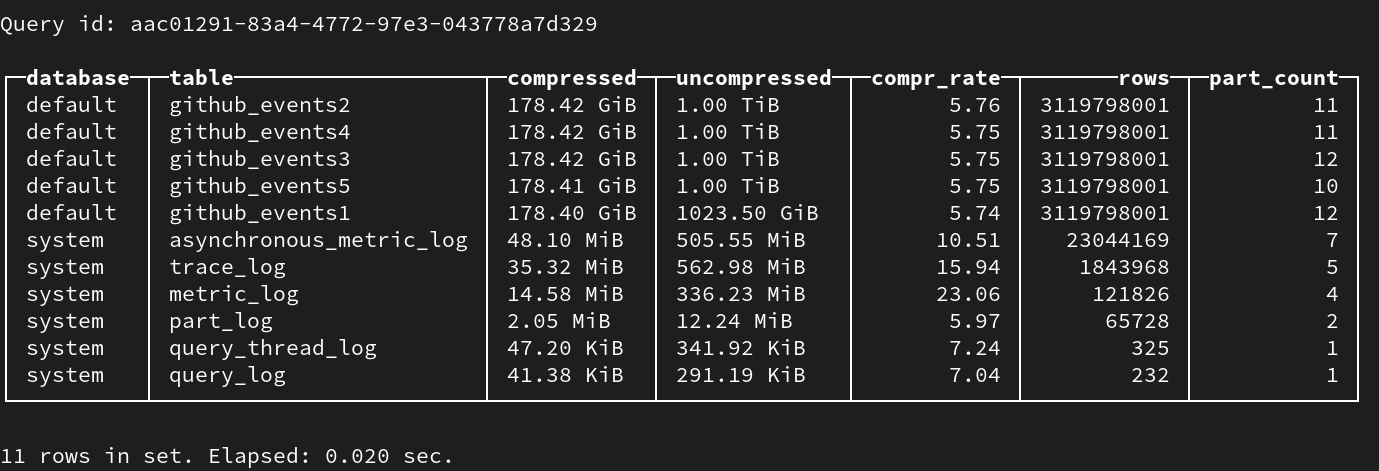
\includegraphics[width=.9\linewidth]{figures/clickhouse/restore3_tables.png}
\end{center}

It appears that the recovery was successful!

 \section{\texttt{clickhouse-backup} performance test}
\label{app:chbk-perf}
While backing up and uploading a backup to remote storage
seemed to work fine (see \ref{app:ch-perf}),
we were unable to actually recover from the backup.
Several attempts were made at restoring from or downloading the remote backups.
All were unsuccessful.
Errors occured during the download phase of the recovery.

An attempt was made to back up up a single table,
upload it to remote storage and then restore from it.
This attempt was successful, but only used a tiny amount of data.
This, and the fact that we were able to list remote backups,
indicates that the configuration/connection to the remote storage itself was probably fine.

Unfortunately, we were not able to perform a proper
performance test of \texttt{clickhouse-backup} with 1TB of data.

\subsection{Recovery with \texttt{clickhouse-backup} (first set of attempts)}
\label{sec:org4d2ee6b}
\subsubsection{Rebuild VM}
\label{sec:org0452162}
Delete VM:
\begin{minted}[breaklines=true,breakanywhere=true]{powershell}
# Delete the VM
az vm delete --name $CHName --resource-group $RGName --yes

# Get all resources in resource group
$resources = az resource list --resource-group $RGName | ConvertFrom-Json -AsHashtable

# Fetch only the ids of resources with names containing "Clickhouse".
$filtered = foreach($r in $resources) {
    Write-Output $r["id"] | grep Clickhouse
}

# Delete the resources
$filtered | % {Remove-AzResource -ResourceId $_ -Force}
$filtered | % {Remove-AzResource -ResourceId $_ -Force}
\end{minted}

Create VM:
\begin{minted}[breaklines=true,breakanywhere=true]{powershell}
az vm create `
    --resource-group $RGName `
    --name $CHName `
    --image Canonical:UbuntuServer:16.04-LTS:16.04.202109280 `
    --admin-username azureuser `
    --size Standard_D4s_v4 `
    --os-disk-size-gb 2048 `
    --ssh-key-values $SSHPath `
    --public-ip-sku Standard
\end{minted}

Install ClickHouse:
\begin{minted}[breaklines=true,breakanywhere=true]{bash}
sudo apt-get install -y apt-transport-https ca-certificates dirmngr
sudo apt-key adv --keyserver hkp://keyserver.ubuntu.com:80 --recv 8919F6BD2B48D754

echo "deb https://packages.clickhouse.com/deb stable main" | sudo tee \
    /etc/apt/sources.list.d/clickhouse.list
sudo apt-get update

sudo apt-get install -y clickhouse-server clickhouse-client

sudo clickhouse start
sudo service clickhouse-server start
\end{minted}

Install \texttt{clickhouse-backup}:
\begin{minted}[breaklines=true,breakanywhere=true]{bash}
# Download archive containing binary
wget https://github.com/AlexAkulov/clickhouse-backup/releases/download/v1.3.2/clickhouse-backup-linux-amd64.tar.gz

# Decompress archive
tar -zxvf clickhouse-backup-linux-amd64.tar.gz

# Move binary to home directory
mv build/linux/amd64/clickhouse-backup ~

# Cleanup
rmdir -p build/linux/amd64
rm clickhouse-backup-linux-amd64.tar.gz
\end{minted}

\texttt{config.yaml} was copied from the test environment (see \ref{app:ch-perf}).

\texttt{config.yaml}:
\begin{minted}[breaklines=true,breakanywhere=true]{yaml}
general:
  remote_storage: azblob
  max_file_size: 0
  disable_progress_bar: false
  backups_to_keep_local: 0
  backups_to_keep_remote: 0
  log_level: info
  allow_empty_backups: false
  download_concurrency: 1
  upload_concurrency: 1
  restore_schema_on_cluster: ""
  upload_by_part: true
  download_by_part: true
clickhouse:
  username: default
  password: ""
  host: localhost
  port: 9000
  disk_mapping: {}
  skip_tables:
  - system.*
  - INFORMATION_SCHEMA.*
  - information_schema.*
  timeout: 5m
  freeze_by_part: false
  secure: false
  skip_verify: false
  sync_replicated_tables: false
  log_sql_queries: true
  config_dir: /etc/clickhouse-server/
  restart_command: systemctl restart clickhouse-server
  ignore_not_exists_error_during_freeze: true
  tls_key: ""
  tls_cert: ""
  tls_ca: ""
  debug: false
s3:
  access_key: ""
  secret_key: ""
  bucket: ""
  endpoint: ""
  region: us-east-1
  acl: private
  assume_role_arn: ""
  force_path_style: false
  path: ""
  disable_ssl: false
  compression_level: 1
  compression_format: tar
  sse: ""
  disable_cert_verification: false
  storage_class: STANDARD
  concurrency: 1
  part_size: 0
  max_parts_count: 10000
  debug: false
gcs:
  credentials_file: ""
  credentials_json: ""
  bucket: ""
  path: ""
  compression_level: 1
  compression_format: tar
  debug: false
  endpoint: ""
cos:
  url: ""
  timeout: 2m
  secret_id: ""
  secret_key: ""
  path: ""
  compression_format: tar
  compression_level: 1
  debug: false
api:
  listen: localhost:7171
  enable_metrics: true
  enable_pprof: false
  username: ""
  password: ""
  secure: false
  certificate_file: ""
  private_key_file: ""
  create_integration_tables: false
  allow_parallel: false
ftp:
  address: ""
  timeout: 2m
  username: ""
  password: ""
  tls: false
  path: ""
  compression_format: tar
  compression_level: 1
  concurrency: 1
  debug: false
sftp:
  address: ""
  port: 22
  username: ""
  password: ""
  key: ""
  path: ""
  compression_format: tar
  compression_level: 1
  concurrency: 1
  debug: false
azblob:
  endpoint_suffix: core.windows.net
  account_name: "perfchbksa"
  account_key: "EIhee0y3zertAVbAa7cRAhYQ/2Oui25vdr6DoL05qkA+CfZZpFMlabzJFPtJG8Xdc735PAbA8w8r+AStl89ieA=="
  sas: "se=2022-05-18&sp=racwdl&sv=2021-04-10&sr=c&skoid=d404139d-e156-421c-9450-19e9734a8141&sktid=09a10672-822f-4467-a5ba-5bb375967c05&skt=2022-05-11T07%3A01%3A18Z&ske=2022-05-18T00%3A00%3A00Z&sks=b&skv=2021-04-10&sig=GgFsZifUWr0r71gCZaD9PbxRXrybhWS09Hpb2scfsKg%3D"
  use_managed_identity: false
  container: "chbkperfcontainer"
  path: "https://perfchbksa.blob.core.windows.net/chbkperfcontainer"
  compression_level: 1
  compression_format: tar
  sse_key: ""
  buffer_size: 0
  buffer_count: 3
  max_parts_count: 1
\end{minted}
\subsubsection{Try to restore from remote backup}
\label{sec:org5cb0fa6}
Bash commands were performed as root in \path{/home/azureuser}.
SQL statements were performed in \texttt{clickhouse-client}.

Showing the tables in the database (no tables):
\begin{minted}[breaklines=true,breakanywhere=true]{sql}
SHOW TABLES

-- Query id: e41781d1-477e-4d48-be0c-73e3b5f26eaa
--
-- Ok.
--
-- 0 rows in set. Elapsed: 0.002 sec.
\end{minted}

Listing remote backups:
\begin{minted}[breaklines=true,breakanywhere=true]{bash}
./clickhouse-backup list remote --config ./config.yaml
# 2022/05/12 09:39:48.379024  info SELECT max(toInt64(bytes_on_disk * 1.02)) AS max_file_size FROM system.parts
# 2022-05-11T07-25-16   895.29GiB   11/05/2022 10:44:05   remote      tar
\end{minted}

Restoring from the remote backup:
\begin{minted}[breaklines=true,breakanywhere=true]{bash}
time ./clickhouse-backup restore_remote 2022-05-11T07-25-16 --config ./config.yaml

# 2022/05/12 09:48:21.324699  info SELECT value FROM `system`.`build_options` where name='VERSION_INTEGER'
# 2022/05/12 09:48:21.326557  info SELECT * FROM system.disks;
# 2022/05/12 09:48:21.332100  info SELECT max(toInt64(bytes_on_disk * 1.02)) AS max_file_size FROM system.parts
# 2022/05/12 09:48:21.459701  info done                      backup=2022-05-11T07-25-16 duration=54ms operation=download size=3.36KiB table_metadata=default.github_events1
# 2022/05/12 09:48:21.507383  info done                      backup=2022-05-11T07-25-16 duration=48ms operation=download size=3.32KiB table_metadata=default.github_events2
# 2022/05/12 09:48:21.512022  info done                      backup=2022-05-11T07-25-16 duration=5ms operation=download size=3.36KiB table_metadata=default.github_events3
# 2022/05/12 09:48:21.516128  info done                      backup=2022-05-11T07-25-16 duration=4ms operation=download size=3.32KiB table_metadata=default.github_events4
# 2022/05/12 09:48:21.520984  info done                      backup=2022-05-11T07-25-16 duration=5ms operation=download size=3.28KiB table_metadata=default.github_events5
# 2022/05/12 09:49:21.524887 error can't acquire semaphore during downloadTableData: context canceled---------]  57.67% 59s
# 2022/05/12 09:49:21.642779 error can't acquire semaphore during Download: context canceled backup=2022-05-11T07-25-16 operation=download
# 2022/05/12 09:50:21.672318 error can't acquire semaphore during downloadTableData: context canceled---------]   8.04% 59s
# 2022/05/12 09:50:21.770237 error one of Download go-routine return error: one of downloadTableData go-routine return error: handling file: /all_3441_4218_4/file_time.bin: context deadline exceeded
#
# real    2m0.461s
# user    0m10.068s
# sys     0m14.108s
\end{minted}

The restoration failed.
\subsubsection{Try to download remote backup}
\label{sec:org8b2d881}
Since \texttt{clickhouse-backup restore\_remote} failed,
we tried to instead download the backup first, and then restore afterwards.
This also failed with the same error.

\begin{minted}[breaklines=true,breakanywhere=true]{bash}
time ./clickhouse-backup download 2022-05-11T07-25-16 --config ./config.yaml

# 2022/05/12 10:00:42.788222  info SELECT value FROM `system`.`build_options` where name='VERSION_INTEGER'
# 2022/05/12 10:00:42.790756  info SELECT * FROM system.disks;
# 2022/05/12 10:00:42.797256  info SELECT max(toInt64(bytes_on_disk * 1.02)) AS max_file_size FROM system.parts
# 2022/05/12 10:00:42.846572  info done                      backup=2022-05-11T07-25-16 duration=5ms operation=download size=3.36KiB table_metadata=default.github_events1
# 2022/05/12 10:00:42.853218  info done                      backup=2022-05-11T07-25-16 duration=7ms operation=download size=3.32KiB table_metadata=default.github_events2
# 2022/05/12 10:00:42.857772  info done                      backup=2022-05-11T07-25-16 duration=4ms operation=download size=3.36KiB table_metadata=default.github_events3
# 2022/05/12 10:00:42.864379  info done                      backup=2022-05-11T07-25-16 duration=7ms operation=download size=3.32KiB table_metadata=default.github_events4
# 2022/05/12 10:00:42.869284  info done                      backup=2022-05-11T07-25-16 duration=5ms operation=download size=3.28KiB table_metadata=default.github_events5
# 2022/05/12 10:01:42.873871 error can't acquire semaphore during downloadTableData: context canceled---------]  63.84% 59s
# 2022/05/12 10:01:42.966195 error can't acquire semaphore during Download: context canceled backup=2022-05-11T07-25-16 operation=download
# 2022/05/12 10:02:43.002110 error can't acquire semaphore during downloadTableData: context canceled---------]   8.08% 59s
# 2022/05/12 10:02:43.087969 error one of Download go-routine return error: one of downloadTableData go-routine return error: handling file: /all_3441_4218_4/file_time.bin: context deadline exceeded
#
# real    2m0.314s
# user    0m10.550s
# sys     0m12.509s
\end{minted}
\subsubsection{Rebuild VM again}
\label{sec:org56a63e8}
The VM was once again rebuilt,
in the same way as in \hyperref[sec:org0452162]{Rebuild VM}.
\subsubsection{Download remote backup again (third attempt)}
\label{sec:org3f5a3c3}
Tried to download the remote backup again, like in \hyperref[sec:org8b2d881]{Try to download remote backup},
but it failed once again.
\subsection{Recovery with \texttt{clickhouse-backup} (second set of attempts)}
\label{sec:orgfaf1fce}
We had another go at restoring from the remote \texttt{clickhouse-backup} backups.
Downloading/restoring from remote backups
failed once again, and we were not sure what to do about it.

We made an attempt at uploading a very small backup to remote storage and then recovering from it.
This worked fine.

Finally, we made an attempt at recovering from the local version of the remote backup.
This worked well.
The restoration took only 2.687 seconds.

\subsubsection{Restore VM}
\label{sec:org46296f4}
The VM was restored via Azure Backup.
This process is the same as in [cref].
\subsubsection{Drop tables}
\label{sec:org5bece9d}
Make it possible to drop tables (had to be run between drop table statements):
\begin{minted}[breaklines=true,breakanywhere=true]{bash}
sudo touch '/var/lib/clickhouse/flags/force_drop_table' && sudo chmod 666 '/var/lib/clickhouse/flags/force_drop_table'
\end{minted}

\begin{minted}[breaklines=true,breakanywhere=true]{sql}
DROP TABLE github_events1
DROP TABLE github_events2
DROP TABLE github_events3
DROP TABLE github_events4
DROP TABLE github_events5
\end{minted}
\subsubsection{Download backup}
\label{sec:org25a0557}
Commands were performed as root.

List remote backups:
\begin{minted}[breaklines=true,breakanywhere=true]{bash}
./clickhouse-backup list remote --config config.yaml
# 2022/05/14 10:00:29.509778  info SELECT max(toInt64(bytes_on_disk * 1.02)) AS max_file_size FROM system.parts
# 2022-05-11T07-25-16   895.29GiB   11/05/2022 10:44:05   remote      tar
\end{minted}

Drop
\begin{minted}[breaklines=true,breakanywhere=true]{bash}
./clickhouse-backup delete local 2022-05-11T07-25-16
\end{minted}

Restore from remote backup:
\begin{minted}[breaklines=true,breakanywhere=true]{bash}
time ./clickhouse-backup restore_remote 2022-05-11T07-25-16 --config config.yaml
# 2022/05/14 10:04:26.068449  info SELECT value FROM `system`.`build_options` where name='VERSION_INTEGER'
# 2022/05/14 10:04:26.071514  info SELECT * FROM system.disks;
# 2022/05/14 10:04:26.078712  info SELECT max(toInt64(bytes_on_disk * 1.02)) AS max_file_size FROM system.parts
# 2022/05/14 10:04:26.202816  info done                      backup=2022-05-11T07-25-16 duration=54ms operation=download size=3.36KiB table_metadata=default.github_events1
# 2022/05/14 10:04:26.207742  info done                      backup=2022-05-11T07-25-16 duration=5ms operation=download size=3.32KiB table_metadata=default.github_events2
# 2022/05/14 10:04:26.220053  info done                      backup=2022-05-11T07-25-16 duration=12ms operation=download size=3.36KiB table_metadata=default.github_events3
# 2022/05/14 10:04:26.225487  info done                      backup=2022-05-11T07-25-16 duration=5ms operation=download size=3.32KiB table_metadata=default.github_events4
# 2022/05/14 10:04:26.230170  info done                      backup=2022-05-11T07-25-16 duration=5ms operation=download size=3.28KiB table_metadata=default.github_events5
# 2022/05/14 10:05:26.234385 error can't acquire semaphore during downloadTableData: context canceled---------]  66.83% 59s
# 2022/05/14 10:05:26.314936 error can't acquire semaphore during Download: context canceled backup=2022-05-11T07-25-16 operation=download
# 2022/05/14 10:06:26.354581 error can't acquire semaphore during downloadTableData: context canceled---------]   9.17% 59s
# 2022/05/14 10:06:26.452971 error one of Download go-routine return error: one of downloadTableData go-routine return error: handling file: /all_3441_4218_4/merge_commit_sha.bin: context deadline exceeded
#
# real    2m0.400s
# user    0m11.283s
# sys     0m14.051s
\end{minted}
\subsubsection{Test with a smaller amount of data (not measuring performance)}
\label{sec:orgbd12c9f}
We did a test where we backup up and recovered a small amount of data,
to prove that the configuration was valid.

Create empty table:
\begin{minted}[breaklines=true,breakanywhere=true]{sql}
CREATE TABLE github_events1
(
    file_time DateTime,
    event_type Enum('CommitCommentEvent' = 1, 'CreateEvent' = 2, 'DeleteEvent' = 3, 'ForkEvent' = 4,
                    'GollumEvent' = 5, 'IssueCommentEvent' = 6, 'IssuesEvent' = 7, 'MemberEvent' = 8,
                    'PublicEvent' = 9, 'PullRequestEvent' = 10, 'PullRequestReviewCommentEvent' = 11,
                    'PushEvent' = 12, 'ReleaseEvent' = 13, 'SponsorshipEvent' = 14, 'WatchEvent' = 15,
                    'GistEvent' = 16, 'FollowEvent' = 17, 'DownloadEvent' = 18, 'PullRequestReviewEvent' = 19,
                    'ForkApplyEvent' = 20, 'Event' = 21, 'TeamAddEvent' = 22),
    actor_login LowCardinality(String),
    repo_name LowCardinality(String),
    created_at DateTime,
    updated_at DateTime,
    action Enum('none' = 0, 'created' = 1, 'added' = 2, 'edited' = 3, 'deleted' = 4, 'opened' = 5, 'closed' = 6, 'reopened' = 7, 'assigned' = 8, 'unassigned' = 9,
                'labeled' = 10, 'unlabeled' = 11, 'review_requested' = 12, 'review_request_removed' = 13, 'synchronize' = 14, 'started' = 15, 'published' = 16, 'update' = 17, 'create' = 18, 'fork' = 19, 'merged' = 20),
    comment_id UInt64,
    body String,
    path String,
    position Int32,
    line Int32,
    ref LowCardinality(String),
    ref_type Enum('none' = 0, 'branch' = 1, 'tag' = 2, 'repository' = 3, 'unknown' = 4),
    creator_user_login LowCardinality(String),
    number UInt32,
    title String,
    labels Array(LowCardinality(String)),
    state Enum('none' = 0, 'open' = 1, 'closed' = 2),
    locked UInt8,
    assignee LowCardinality(String),
    assignees Array(LowCardinality(String)),
    comments UInt32,
    author_association Enum('NONE' = 0, 'CONTRIBUTOR' = 1, 'OWNER' = 2, 'COLLABORATOR' = 3, 'MEMBER' = 4, 'MANNEQUIN' = 5),
    closed_at DateTime,
    merged_at DateTime,
    merge_commit_sha String,
    requested_reviewers Array(LowCardinality(String)),
    requested_teams Array(LowCardinality(String)),
    head_ref LowCardinality(String),
    head_sha String,
    base_ref LowCardinality(String),
    base_sha String,
    merged UInt8,
    mergeable UInt8,
    rebaseable UInt8,
    mergeable_state Enum('unknown' = 0, 'dirty' = 1, 'clean' = 2, 'unstable' = 3, 'draft' = 4),
    merged_by LowCardinality(String),
    review_comments UInt32,
    maintainer_can_modify UInt8,
    commits UInt32,
    additions UInt32,
    deletions UInt32,
    changed_files UInt32,
    diff_hunk String,
    original_position UInt32,
    commit_id String,
    original_commit_id String,
    push_size UInt32,
    push_distinct_size UInt32,
    member_login LowCardinality(String),
    release_tag_name String,
    release_name String,
    review_state Enum('none' = 0, 'approved' = 1, 'changes_requested' = 2, 'commented' = 3, 'dismissed' = 4, 'pending' = 5)
)
ENGINE = MergeTree
ORDER BY (event_type, repo_name, created_at)
\end{minted}

Create local backup:
\begin{minted}[breaklines=true,breakanywhere=true]{bash}
./clickhouse-backup create
# 2022/05/14 10:12:59.474330  info SELECT name, engine FROM system.databases WHERE name NOT IN ('system', 'INFORMATION_SCHE
# MA', 'information_schema')
# 2022/05/14 10:12:59.477846  info SHOW CREATE DATABASE `default`
# 2022/05/14 10:12:59.481048  info SELECT count() FROM system.settings WHERE name = 'show_table_uuid_in_table_create_query_
# if_not_nil'
# 2022/05/14 10:12:59.483473  info SELECT name FROM system.databases WHERE engine IN ('MySQL','PostgreSQL')
# 2022/05/14 10:12:59.485660  info
#                 SELECT
#                         countIf(name='data_path') is_data_path_present,
#                         countIf(name='data_paths') is_data_paths_present,
#                         countIf(name='uuid') is_uuid_present,
#                         countIf(name='create_table_query') is_create_table_query_present,
#                         countIf(name='total_bytes') is_total_bytes_present
#                 FROM system.columns WHERE database='system' AND table='tables'
#
# 2022/05/14 10:12:59.488383  info SELECT database, name, engine , data_paths , uuid , create_table_query , coalesce(total_
# bytes, 0) AS total_bytes   FROM system.tables WHERE is_temporary = 0 SETTINGS show_table_uuid_in_table_create_query_if_no
# t_nil=1
# 2022/05/14 10:12:59.496461  info SELECT sum(bytes_on_disk) as size FROM system.parts WHERE database='default' AND table='
# github_events1' GROUP BY database, table
# 2022/05/14 10:12:59.502336  info SELECT value FROM `system`.`build_options` where name='VERSION_INTEGER'
# 2022/05/14 10:12:59.505121  info SELECT * FROM system.disks;
# 2022/05/14 10:12:59.508045  info ALTER TABLE `default`.`github_events1` FREEZE WITH NAME 'b380781a01ec426e8493f83f940e7f5
# 8';
# 2022/05/14 10:12:59.624218  info done                      backup=2022-05-14T10-12-59 operation=create table=default.gith
# ub_events1
\end{minted}

List backup:
\begin{minted}[breaklines=true,breakanywhere=true]{bash}
./clickhouse-backup list
# 2022/05/14 10:13:19.784137  info SELECT value FROM `system`.`build_options` where name='VERSION_INTEGER'
# 2022/05/14 10:13:19.787608  info SELECT * FROM system.disks;
# 2022-05-14T10-12-59   2.81KiB   14/05/2022 10:12:59   local
\end{minted}

Upload backup to remote storage:
\begin{minted}[breaklines=true,breakanywhere=true]{bash}
./clickhouse-backup upload 2022-05-14T10-12-59 -c config.yaml
\end{minted}

Delete local backup:
\begin{minted}[breaklines=true,breakanywhere=true]{bash}
./clickhouse-backup delete local 2022-05-14T10-12-59
# 2022/05/14 10:18:24.470651  info SELECT value FROM `system`.`build_options` where name='VERSION_INTEGER'
# 2022/05/14 10:18:24.472547  info SELECT * FROM system.disks;
# 2022/05/14 10:18:24.476090  info done                      backup=2022-05-14T10-12-59 duration=8ms location=local operation=delete
\end{minted}

Drop the table:
\begin{minted}[breaklines=true,breakanywhere=true]{sql}
DROP TABLE github_events1
\end{minted}

Restore from remote backup:
\begin{minted}[breaklines=true,breakanywhere=true]{bash}
./clickhouse-backup restore_remote 2022-05-14T10-12-59 -c config.yaml
# 2022/05/14 10:20:05.358861  info SELECT value FROM `system`.`build_options` where name='VERSION_INTEGER'
# 2022/05/14 10:20:05.360724  info SELECT * FROM system.disks;
# 2022/05/14 10:20:05.368823  info SELECT max(toInt64(bytes_on_disk * 1.02)) AS max_file_size FROM system.parts
# 2022/05/14 10:20:05.425455  info done                      backup=2022-05-14T10-12-59 duration=5ms operation=download size=2.81KiB table_metadata=default.github_events1
# 2022/05/14 10:20:05.425540  info done                      diff_parts=0 duration=0s operation=downloadDiffParts
# 2022/05/14 10:20:05.425578  info done                      backup=2022-05-14T10-12-59 duration=0s operation=download_data size=0B table=default.github_events1
# 2022/05/14 10:20:05.433103  info done                      backup=2022-05-14T10-12-59 duration=70ms operation=download size=2.81KiB
# 2022/05/14 10:20:05.436457  info SELECT value FROM `system`.`build_options` where name='VERSION_INTEGER'
# 2022/05/14 10:20:05.439819  info SELECT * FROM system.disks;
# 2022/05/14 10:20:05.442308  info CREATE DATABASE IF NOT EXISTS default
# ENGINE = Atomic
# 2022/05/14 10:20:05.443762  info SELECT engine FROM system.databases WHERE name = 'default'
# 2022/05/14 10:20:05.447623  info DROP TABLE IF EXISTS `default`.`github_events1` NO DELAY
# 2022/05/14 10:20:05.451154  info CREATE DATABASE IF NOT EXISTS `default`
# 2022/05/14 10:20:05.452970  info CREATE TABLE default.github_events1 UUID '8742d240-9dc9-4a43-89d0-f06e9eac0b61' (`file_time` DateTime, `event_type` Enum8('CommitCommentEvent' = 1, 'CreateEvent' = 2, 'DeleteEvent' = 3, 'ForkEvent' = 4, 'GollumEvent' = 5, 'IssueCommentEvent' = 6, 'IssuesEvent' = 7, 'MemberEvent' = 8, 'PublicEvent' = 9, 'PullRequestEvent' = 10, 'PullRequestReviewCommentEvent' = 11, 'PushEvent' = 12, 'ReleaseEvent' = 13, 'SponsorshipEvent' = 14, 'WatchEvent' = 15, 'GistEvent' = 16, 'FollowEvent' = 17, 'DownloadEvent' = 18, 'PullRequestReviewEvent' = 19, 'ForkApplyEvent' = 20, 'Event' = 21, 'TeamAddEvent' = 22), `actor_login` LowCardinality(String), `repo_name` LowCardinality(String), `created_at` DateTime, `updated_at` DateTime, `action` Enum8('none' = 0, 'created' = 1, 'added' = 2, 'edited' = 3, 'deleted' = 4, 'opened' = 5, 'closed' = 6, 'reopened' = 7, 'assigned' = 8, 'unassigned' = 9, 'labeled' = 10, 'unlabeled' = 11, 'review_requested' = 12, 'review_request_removed' = 13, 'synchronize' = 14, 'started' = 15, 'published' = 16, 'update' = 17, 'create' = 18, 'fork' = 19, 'merged' = 20), `comment_id` UInt64, `body` String, `path` String, `position` Int32, `line` Int32, `ref` LowCardinality(String), `ref_type` Enum8('none' = 0, 'branch' = 1, 'tag' = 2, 'repository' = 3, 'unknown' = 4), `creator_user_login` LowCardinality(String), `number` UInt32, `title` String, `labels` Array(LowCardinality(String)), `state` Enum8('none' = 0, 'open' = 1, 'closed' = 2), `locked` UInt8, `assignee` LowCardinality(String), `assignees` Array(LowCardinality(String)), `comments` UInt32, `author_association` Enum8('NONE' = 0, 'CONTRIBUTOR' = 1, 'OWNER' = 2, 'COLLABORATOR' = 3, 'MEMBER' = 4, 'MANNEQUIN' = 5), `closed_at` DateTime, `merged_at` DateTime, `merge_commit_sha` String, `requested_reviewers` Array(LowCardinality(String)), `requested_teams` Array(LowCardinality(String)), `head_ref` LowCardinality(String), `head_sha` String, `base_ref` LowCardinality(String), `base_sha` String, `merged` UInt8, `mergeable` UInt8, `rebaseable` UInt8, `mergeable_state` Enum8('unknown' = 0, 'dirty' = 1, 'clean' = 2, 'unstable' = 3, 'draft' = 4), `merged_by` LowCardinality(String), `review_comments` UInt32, `maintainer_can_modify` UInt8, `commits` UInt32, `additions` UInt32, `deletions` UInt32, `changed_files` UInt32, `diff_hunk` String, `original_position` UInt32, `commit_id` String, `original_commit_id` String, `push_size` UInt32, `push_distinct_size` UInt32, `member_login` LowCardinality(String), `release_tag_name` String, `release_name` String, `review_state` Enum8('none' = 0, 'approved' = 1, 'changes_requested' = 2, 'commented' = 3, 'dismissed' = 4, 'pending' = 5)) ENGINE = MergeTree ORDER BY (event_type, repo_name, created_at) SETTINGS index_granularity = 8192
# 2022/05/14 10:20:05.527062  info SELECT count() FROM system.settings WHERE name = 'show_table_uuid_in_table_create_query_if_not_nil'
# 2022/05/14 10:20:05.544058  info SELECT name FROM system.databases WHERE engine IN ('MySQL','PostgreSQL')
# 2022/05/14 10:20:05.546963  info
# 		SELECT
# 			countIf(name='data_path') is_data_path_present,
# 			countIf(name='data_paths') is_data_paths_present,
# 			countIf(name='uuid') is_uuid_present,
# 			countIf(name='create_table_query') is_create_table_query_present,
# 			countIf(name='total_bytes') is_total_bytes_present
# 		FROM system.columns WHERE database='system' AND table='tables'
#
# 2022/05/14 10:20:05.568889  info SELECT database, name, engine , data_paths , uuid , create_table_query , coalesce(total_bytes, 0) AS total_bytes   FROM system.tables WHERE is_temporary = 0 SETTINGS show_table_uuid_in_table_create_query_if_not_nil=1
# 2022/05/14 10:20:05.578972  info SELECT sum(bytes_on_disk) as size FROM system.parts WHERE database='default' AND table='github_events1' GROUP BY database, table
# 2022/05/14 10:20:05.582682  info done                      backup=2022-05-14T10-12-59 operation=restore table=default.github_events1
# 2022/05/14 10:20:05.582734  info done                      backup=2022-05-14T10-12-59 duration=59ms operation=restore
# 2022/05/14 10:20:05.582763  info done                      backup=2022-05-14T10-12-59 operation=restore
\end{minted}
\subsubsection{Attempt to restore from local backups}
\label{sec:org6d27792}
The VM was restored with Azure Backup, in order to recover the local backup.

The restore was timed with \texttt{time}.
It took 2.687 seconds.

\begin{minted}[breaklines=true,breakanywhere=true]{bash}
./clickhouse-backup list
# 2022/05/14 10:47:31.108857  info SELECT value FROM `system`.`build_options` where name='VERSION_INTEGER'
# 2022/05/14 10:47:31.112370  info SELECT * FROM system.disks;
# 2022-05-11T07-25-16   895.28GiB   11/05/2022 07:25:17   local
\end{minted}

In \texttt{clickhouse-client}, all tables were dropped:
\begin{minted}[breaklines=true,breakanywhere=true]{sql}
DROP TABLE github_events1
DROP TABLE github_events2
DROP TABLE github_events3
DROP TABLE github_events4
DROP TABLE github_events5
\end{minted}

Before each drop table statement, the following command had to be run in bash:
\begin{minted}[breaklines=true,breakanywhere=true]{bash}
sudo touch '/var/lib/clickhouse/flags/force_drop_table' && sudo chmod 666 '/var/lib/clickhouse/flags/force_drop_table'
\end{minted}

Show tables:
\begin{minted}[breaklines=true,breakanywhere=true]{sql}
SHOW TABLES

-- Query id: d104549f-c266-498a-a1c2-07dc85f9ea0e
--
-- Ok.
--
-- 0 rows in set. Elapsed: 0.002 sec.
\end{minted}

ClickHouse was restarted with \texttt{clickhouse restart} before restoring from backup.

Measure time to restore from local backup:
\begin{minted}[breaklines=true,breakanywhere=true]{bash}
time ./clickhouse-backup restore 2022-05-11T07-25-16
# 2022/05/14 11:03:48.480915  info SELECT value FROM `system`.`build_options` where name='VERSION_INTEGER'
# 2022/05/14 11:03:48.484637  info SELECT * FROM system.disks;
# 2022/05/14 11:03:48.490860  info CREATE DATABASE IF NOT EXISTS default
# ENGINE = Atomic
# 2022/05/14 11:03:48.492717  info SELECT engine FROM system.databases WHERE name = 'default'
# 2022/05/14 11:03:48.495213  info DROP TABLE IF EXISTS `default`.`github_events1` NO DELAY
# 2022/05/14 11:03:48.496391  info SELECT engine FROM system.databases WHERE name = 'default'
# 2022/05/14 11:03:48.499202  info DROP TABLE IF EXISTS `default`.`github_events2` NO DELAY
# 2022/05/14 11:03:48.504034  info SELECT engine FROM system.databases WHERE name = 'default'
# 2022/05/14 11:03:48.509525  info DROP TABLE IF EXISTS `default`.`github_events3` NO DELAY
# 2022/05/14 11:03:48.510781  info SELECT engine FROM system.databases WHERE name = 'default'
# 2022/05/14 11:03:48.515357  info DROP TABLE IF EXISTS `default`.`github_events4` NO DELAY
# 2022/05/14 11:03:48.516841  info SELECT engine FROM system.databases WHERE name = 'default'
# 2022/05/14 11:03:48.519688  info DROP TABLE IF EXISTS `default`.`github_events5` NO DELAY
# 2022/05/14 11:03:48.522352  info CREATE DATABASE IF NOT EXISTS `default`
# 2022/05/14 11:03:48.523692  info CREATE TABLE default.github_events1 UUID '1711c114-1286-4a0b-8f9a-11fbc6d35b89' (`file_time` DateTime, `event_type` Enum8('CommitCommentEvent' = 1, 'CreateEvent' = 2, 'DeleteEvent' = 3, 'ForkEvent' = 4, 'GollumEvent' = 5, 'IssueCommentEvent' = 6, 'IssuesEvent' = 7, 'MemberEvent' = 8, 'PublicEvent' = 9, 'PullRequestEvent' = 10, 'PullRequestReviewCommentEvent' = 11, 'PushEvent' = 12, 'ReleaseEvent' = 13, 'SponsorshipEvent' = 14, 'WatchEvent' = 15, 'GistEvent' = 16, 'FollowEvent' = 17, 'DownloadEvent' = 18, 'PullRequestReviewEvent' = 19, 'ForkApplyEvent' = 20, 'Event' = 21, 'TeamAddEvent' = 22), `actor_login` LowCardinality(String), `repo_name` LowCardinality(String), `created_at` DateTime, `updated_at` DateTime, `action` Enum8('none' = 0, 'created' = 1, 'added' = 2, 'edited' = 3, 'deleted' = 4, 'opened' = 5, 'closed' = 6, 'reopened' = 7, 'assigned' = 8, 'unassigned' = 9, 'labeled' = 10, 'unlabeled' = 11, 'review_requested' = 12, 'review_request_removed' = 13, 'synchronize' = 14, 'started' = 15, 'published' = 16, 'update' = 17, 'create' = 18, 'fork' = 19, 'merged' = 20), `comment_id` UInt64, `body` String, `path` String, `position` Int32, `line` Int32, `ref` LowCardinality(String), `ref_type` Enum8('none' = 0, 'branch' = 1, 'tag' = 2, 'repository' = 3, 'unknown' = 4), `creator_user_login` LowCardinality(String), `number` UInt32, `title` String, `labels` Array(LowCardinality(String)), `state` Enum8('none' = 0, 'open' = 1, 'closed' = 2), `locked` UInt8, `assignee` LowCardinality(String), `assignees` Array(LowCardinality(String)), `comments` UInt32, `author_association` Enum8('NONE' = 0, 'CONTRIBUTOR' = 1, 'OWNER' = 2, 'COLLABORATOR' = 3, 'MEMBER' = 4, 'MANNEQUIN' = 5), `closed_at` DateTime, `merged_at` DateTime, `merge_commit_sha` String, `requested_reviewers` Array(LowCardinality(String)), `requested_teams` Array(LowCardinality(String)), `head_ref` LowCardinality(String), `head_sha` String, `base_ref` LowCardinality(String), `base_sha` String, `merged` UInt8, `mergeable` UInt8, `rebaseable` UInt8, `mergeable_state` Enum8('unknown' = 0, 'dirty' = 1, 'clean' = 2, 'unstable' = 3, 'draft' = 4), `merged_by` LowCardinality(String), `review_comments` UInt32, `maintainer_can_modify` UInt8, `commits` UInt32, `additions` UInt32, `deletions` UInt32, `changed_files` UInt32, `diff_hunk` String, `original_position` UInt32, `commit_id` String, `original_commit_id` String, `push_size` UInt32, `push_distinct_size` UInt32, `member_login` LowCardinality(String), `release_tag_name` String, `release_name` String, `review_state` Enum8('none' = 0, 'approved' = 1, 'changes_requested' = 2, 'commented' = 3, 'dismissed' = 4, 'pending' = 5)) ENGINE = MergeTree ORDER BY (event_type, repo_name, created_at) SETTINGS index_granularity = 8192
# 2022/05/14 11:03:48.529620  warn can't create table 'default.github_events1': code: 57, message: Directory for table data store/171/1711c114-1286-4a0b-8f9a-11fbc6d35b89/ already exists, will try again backup=2022-05-11T07-25-16 operation=restore
# 2022/05/14 11:03:48.529647  info CREATE DATABASE IF NOT EXISTS `default`
# 2022/05/14 11:03:48.531904  info CREATE TABLE default.github_events2 UUID '1991bd38-adaf-4691-aa49-c04b27f61485' (`file_time` DateTime, `event_type` Enum8('CommitCommentEvent' = 1, 'CreateEvent' = 2, 'DeleteEvent' = 3, 'ForkEvent' = 4, 'GollumEvent' = 5, 'IssueCommentEvent' = 6, 'IssuesEvent' = 7, 'MemberEvent' = 8, 'PublicEvent' = 9, 'PullRequestEvent' = 10, 'PullRequestReviewCommentEvent' = 11, 'PushEvent' = 12, 'ReleaseEvent' = 13, 'SponsorshipEvent' = 14, 'WatchEvent' = 15, 'GistEvent' = 16, 'FollowEvent' = 17, 'DownloadEvent' = 18, 'PullRequestReviewEvent' = 19, 'ForkApplyEvent' = 20, 'Event' = 21, 'TeamAddEvent' = 22), `actor_login` LowCardinality(String), `repo_name` LowCardinality(String), `created_at` DateTime, `updated_at` DateTime, `action` Enum8('none' = 0, 'created' = 1, 'added' = 2, 'edited' = 3, 'deleted' = 4, 'opened' = 5, 'closed' = 6, 'reopened' = 7, 'assigned' = 8, 'unassigned' = 9, 'labeled' = 10, 'unlabeled' = 11, 'review_requested' = 12, 'review_request_removed' = 13, 'synchronize' = 14, 'started' = 15, 'published' = 16, 'update' = 17, 'create' = 18, 'fork' = 19, 'merged' = 20), `comment_id` UInt64, `body` String, `path` String, `position` Int32, `line` Int32, `ref` LowCardinality(String), `ref_type` Enum8('none' = 0, 'branch' = 1, 'tag' = 2, 'repository' = 3, 'unknown' = 4), `creator_user_login` LowCardinality(String), `number` UInt32, `title` String, `labels` Array(LowCardinality(String)), `state` Enum8('none' = 0, 'open' = 1, 'closed' = 2), `locked` UInt8, `assignee` LowCardinality(String), `assignees` Array(LowCardinality(String)), `comments` UInt32, `author_association` Enum8('NONE' = 0, 'CONTRIBUTOR' = 1, 'OWNER' = 2, 'COLLABORATOR' = 3, 'MEMBER' = 4, 'MANNEQUIN' = 5), `closed_at` DateTime, `merged_at` DateTime, `merge_commit_sha` String, `requested_reviewers` Array(LowCardinality(String)), `requested_teams` Array(LowCardinality(String)), `head_ref` LowCardinality(String), `head_sha` String, `base_ref` LowCardinality(String), `base_sha` String, `merged` UInt8, `mergeable` UInt8, `rebaseable` UInt8, `mergeable_state` Enum8('unknown' = 0, 'dirty' = 1, 'clean' = 2, 'unstable' = 3, 'draft' = 4), `merged_by` LowCardinality(String), `review_comments` UInt32, `maintainer_can_modify` UInt8, `commits` UInt32, `additions` UInt32, `deletions` UInt32, `changed_files` UInt32, `diff_hunk` String, `original_position` UInt32, `commit_id` String, `original_commit_id` String, `push_size` UInt32, `push_distinct_size` UInt32, `member_login` LowCardinality(String), `release_tag_name` String, `release_name` String, `review_state` Enum8('none' = 0, 'approved' = 1, 'changes_requested' = 2, 'commented' = 3, 'dismissed' = 4, 'pending' = 5)) ENGINE = MergeTree ORDER BY (event_type, repo_name, created_at) SETTINGS index_granularity = 8192
# 2022/05/14 11:03:48.535293  warn can't create table 'default.github_events2': code: 57, message: Directory for table data store/199/1991bd38-adaf-4691-aa49-c04b27f61485/ already exists, will try again backup=2022-05-11T07-25-16 operation=restore
# 2022/05/14 11:03:48.535317  info CREATE DATABASE IF NOT EXISTS `default`
# 2022/05/14 11:03:48.537514  info CREATE TABLE default.github_events3 UUID 'c403ed92-213a-4245-b98b-408d6fed9377' (`file_time` DateTime, `event_type` Enum8('CommitCommentEvent' = 1, 'CreateEvent' = 2, 'DeleteEvent' = 3, 'ForkEvent' = 4, 'GollumEvent' = 5, 'IssueCommentEvent' = 6, 'IssuesEvent' = 7, 'MemberEvent' = 8, 'PublicEvent' = 9, 'PullRequestEvent' = 10, 'PullRequestReviewCommentEvent' = 11, 'PushEvent' = 12, 'ReleaseEvent' = 13, 'SponsorshipEvent' = 14, 'WatchEvent' = 15, 'GistEvent' = 16, 'FollowEvent' = 17, 'DownloadEvent' = 18, 'PullRequestReviewEvent' = 19, 'ForkApplyEvent' = 20, 'Event' = 21, 'TeamAddEvent' = 22), `actor_login` LowCardinality(String), `repo_name` LowCardinality(String), `created_at` DateTime, `updated_at` DateTime, `action` Enum8('none' = 0, 'created' = 1, 'added' = 2, 'edited' = 3, 'deleted' = 4, 'opened' = 5, 'closed' = 6, 'reopened' = 7, 'assigned' = 8, 'unassigned' = 9, 'labeled' = 10, 'unlabeled' = 11, 'review_requested' = 12, 'review_request_removed' = 13, 'synchronize' = 14, 'started' = 15, 'published' = 16, 'update' = 17, 'create' = 18, 'fork' = 19, 'merged' = 20), `comment_id` UInt64, `body` String, `path` String, `position` Int32, `line` Int32, `ref` LowCardinality(String), `ref_type` Enum8('none' = 0, 'branch' = 1, 'tag' = 2, 'repository' = 3, 'unknown' = 4), `creator_user_login` LowCardinality(String), `number` UInt32, `title` String, `labels` Array(LowCardinality(String)), `state` Enum8('none' = 0, 'open' = 1, 'closed' = 2), `locked` UInt8, `assignee` LowCardinality(String), `assignees` Array(LowCardinality(String)), `comments` UInt32, `author_association` Enum8('NONE' = 0, 'CONTRIBUTOR' = 1, 'OWNER' = 2, 'COLLABORATOR' = 3, 'MEMBER' = 4, 'MANNEQUIN' = 5), `closed_at` DateTime, `merged_at` DateTime, `merge_commit_sha` String, `requested_reviewers` Array(LowCardinality(String)), `requested_teams` Array(LowCardinality(String)), `head_ref` LowCardinality(String), `head_sha` String, `base_ref` LowCardinality(String), `base_sha` String, `merged` UInt8, `mergeable` UInt8, `rebaseable` UInt8, `mergeable_state` Enum8('unknown' = 0, 'dirty' = 1, 'clean' = 2, 'unstable' = 3, 'draft' = 4), `merged_by` LowCardinality(String), `review_comments` UInt32, `maintainer_can_modify` UInt8, `commits` UInt32, `additions` UInt32, `deletions` UInt32, `changed_files` UInt32, `diff_hunk` String, `original_position` UInt32, `commit_id` String, `original_commit_id` String, `push_size` UInt32, `push_distinct_size` UInt32, `member_login` LowCardinality(String), `release_tag_name` String, `release_name` String, `review_state` Enum8('none' = 0, 'approved' = 1, 'changes_requested' = 2, 'commented' = 3, 'dismissed' = 4, 'pending' = 5)) ENGINE = MergeTree ORDER BY (event_type, repo_name, created_at) SETTINGS index_granularity = 8192
# 2022/05/14 11:03:48.541332  warn can't create table 'default.github_events3': code: 57, message: Directory for table data store/c40/c403ed92-213a-4245-b98b-408d6fed9377/ already exists, will try again backup=2022-05-11T07-25-16 operation=restore
# 2022/05/14 11:03:48.541354  info CREATE DATABASE IF NOT EXISTS `default`
# 2022/05/14 11:03:48.543374  info CREATE TABLE default.github_events4 UUID '6e6a4e02-a9fa-42ad-a0ce-af77e49a2aee' (`file_time` DateTime, `event_type` Enum8('CommitCommentEvent' = 1, 'CreateEvent' = 2, 'DeleteEvent' = 3, 'ForkEvent' = 4, 'GollumEvent' = 5, 'IssueCommentEvent' = 6, 'IssuesEvent' = 7, 'MemberEvent' = 8, 'PublicEvent' = 9, 'PullRequestEvent' = 10, 'PullRequestReviewCommentEvent' = 11, 'PushEvent' = 12, 'ReleaseEvent' = 13, 'SponsorshipEvent' = 14, 'WatchEvent' = 15, 'GistEvent' = 16, 'FollowEvent' = 17, 'DownloadEvent' = 18, 'PullRequestReviewEvent' = 19, 'ForkApplyEvent' = 20, 'Event' = 21, 'TeamAddEvent' = 22), `actor_login` LowCardinality(String), `repo_name` LowCardinality(String), `created_at` DateTime, `updated_at` DateTime, `action` Enum8('none' = 0, 'created' = 1, 'added' = 2, 'edited' = 3, 'deleted' = 4, 'opened' = 5, 'closed' = 6, 'reopened' = 7, 'assigned' = 8, 'unassigned' = 9, 'labeled' = 10, 'unlabeled' = 11, 'review_requested' = 12, 'review_request_removed' = 13, 'synchronize' = 14, 'started' = 15, 'published' = 16, 'update' = 17, 'create' = 18, 'fork' = 19, 'merged' = 20), `comment_id` UInt64, `body` String, `path` String, `position` Int32, `line` Int32, `ref` LowCardinality(String), `ref_type` Enum8('none' = 0, 'branch' = 1, 'tag' = 2, 'repository' = 3, 'unknown' = 4), `creator_user_login` LowCardinality(String), `number` UInt32, `title` String, `labels` Array(LowCardinality(String)), `state` Enum8('none' = 0, 'open' = 1, 'closed' = 2), `locked` UInt8, `assignee` LowCardinality(String), `assignees` Array(LowCardinality(String)), `comments` UInt32, `author_association` Enum8('NONE' = 0, 'CONTRIBUTOR' = 1, 'OWNER' = 2, 'COLLABORATOR' = 3, 'MEMBER' = 4, 'MANNEQUIN' = 5), `closed_at` DateTime, `merged_at` DateTime, `merge_commit_sha` String, `requested_reviewers` Array(LowCardinality(String)), `requested_teams` Array(LowCardinality(String)), `head_ref` LowCardinality(String), `head_sha` String, `base_ref` LowCardinality(String), `base_sha` String, `merged` UInt8, `mergeable` UInt8, `rebaseable` UInt8, `mergeable_state` Enum8('unknown' = 0, 'dirty' = 1, 'clean' = 2, 'unstable' = 3, 'draft' = 4), `merged_by` LowCardinality(String), `review_comments` UInt32, `maintainer_can_modify` UInt8, `commits` UInt32, `additions` UInt32, `deletions` UInt32, `changed_files` UInt32, `diff_hunk` String, `original_position` UInt32, `commit_id` String, `original_commit_id` String, `push_size` UInt32, `push_distinct_size` UInt32, `member_login` LowCardinality(String), `release_tag_name` String, `release_name` String, `review_state` Enum8('none' = 0, 'approved' = 1, 'changes_requested' = 2, 'commented' = 3, 'dismissed' = 4, 'pending' = 5)) ENGINE = MergeTree ORDER BY (event_type, repo_name, created_at) SETTINGS index_granularity = 8192
# 2022/05/14 11:03:48.546649  warn can't create table 'default.github_events4': code: 57, message: Directory for table data store/6e6/6e6a4e02-a9fa-42ad-a0ce-af77e49a2aee/ already exists, will try again backup=2022-05-11T07-25-16 operation=restore
# 2022/05/14 11:03:48.546680  info CREATE DATABASE IF NOT EXISTS `default`
# 2022/05/14 11:03:48.548692  info CREATE TABLE default.github_events5 UUID '697e13ba-37ac-44ac-a7fc-01b0081b4670' (`file_time` DateTime, `event_type` Enum8('CommitCommentEvent' = 1, 'CreateEvent' = 2, 'DeleteEvent' = 3, 'ForkEvent' = 4, 'GollumEvent' = 5, 'IssueCommentEvent' = 6, 'IssuesEvent' = 7, 'MemberEvent' = 8, 'PublicEvent' = 9, 'PullRequestEvent' = 10, 'PullRequestReviewCommentEvent' = 11, 'PushEvent' = 12, 'ReleaseEvent' = 13, 'SponsorshipEvent' = 14, 'WatchEvent' = 15, 'GistEvent' = 16, 'FollowEvent' = 17, 'DownloadEvent' = 18, 'PullRequestReviewEvent' = 19, 'ForkApplyEvent' = 20, 'Event' = 21, 'TeamAddEvent' = 22), `actor_login` LowCardinality(String), `repo_name` LowCardinality(String), `created_at` DateTime, `updated_at` DateTime, `action` Enum8('none' = 0, 'created' = 1, 'added' = 2, 'edited' = 3, 'deleted' = 4, 'opened' = 5, 'closed' = 6, 'reopened' = 7, 'assigned' = 8, 'unassigned' = 9, 'labeled' = 10, 'unlabeled' = 11, 'review_requested' = 12, 'review_request_removed' = 13, 'synchronize' = 14, 'started' = 15, 'published' = 16, 'update' = 17, 'create' = 18, 'fork' = 19, 'merged' = 20), `comment_id` UInt64, `body` String, `path` String, `position` Int32, `line` Int32, `ref` LowCardinality(String), `ref_type` Enum8('none' = 0, 'branch' = 1, 'tag' = 2, 'repository' = 3, 'unknown' = 4), `creator_user_login` LowCardinality(String), `number` UInt32, `title` String, `labels` Array(LowCardinality(String)), `state` Enum8('none' = 0, 'open' = 1, 'closed' = 2), `locked` UInt8, `assignee` LowCardinality(String), `assignees` Array(LowCardinality(String)), `comments` UInt32, `author_association` Enum8('NONE' = 0, 'CONTRIBUTOR' = 1, 'OWNER' = 2, 'COLLABORATOR' = 3, 'MEMBER' = 4, 'MANNEQUIN' = 5), `closed_at` DateTime, `merged_at` DateTime, `merge_commit_sha` String, `requested_reviewers` Array(LowCardinality(String)), `requested_teams` Array(LowCardinality(String)), `head_ref` LowCardinality(String), `head_sha` String, `base_ref` LowCardinality(String), `base_sha` String, `merged` UInt8, `mergeable` UInt8, `rebaseable` UInt8, `mergeable_state` Enum8('unknown' = 0, 'dirty' = 1, 'clean' = 2, 'unstable' = 3, 'draft' = 4), `merged_by` LowCardinality(String), `review_comments` UInt32, `maintainer_can_modify` UInt8, `commits` UInt32, `additions` UInt32, `deletions` UInt32, `changed_files` UInt32, `diff_hunk` String, `original_position` UInt32, `commit_id` String, `original_commit_id` String, `push_size` UInt32, `push_distinct_size` UInt32, `member_login` LowCardinality(String), `release_tag_name` String, `release_name` String, `review_state` Enum8('none' = 0, 'approved' = 1, 'changes_requested' = 2, 'commented' = 3, 'dismissed' = 4, 'pending' = 5)) ENGINE = MergeTree ORDER BY (event_type, repo_name, created_at) SETTINGS index_granularity = 8192
# 2022/05/14 11:03:48.552764 error can't create table `default`.`github_events5`: code: 57, message: Directory for table data store/697/697e13ba-37ac-44ac-a7fc-01b0081b4670/ already exists after 5 times, please check your schema dependencies
#
# real	0m0.089s
# user	0m0.092s
# sys	0m0.022s
\end{minted}

The restore fails because some directories apparently already exist.
The VM was restarted.

New attempt at restoring from a local backup:
\begin{minted}[breaklines=true,breakanywhere=true]{bash}
time ./clickhouse-backup restore 2022-05-11T07-25-16
# 2022/05/14 11:08:27.188612  info SELECT value FROM `system`.`build_options` where name='VERSION_INTEGER'
# 2022/05/14 11:08:27.191239  info SELECT * FROM system.disks;
# 2022/05/14 11:08:27.193861  info CREATE DATABASE IF NOT EXISTS default
# ENGINE = Atomic
# 2022/05/14 11:08:27.195504  info SELECT engine FROM system.databases WHERE name = 'default'
# 2022/05/14 11:08:27.198077  info DROP TABLE IF EXISTS `default`.`github_events1` NO DELAY
# 2022/05/14 11:08:27.200105  info SELECT engine FROM system.databases WHERE name = 'default'
# 2022/05/14 11:08:27.203430  info DROP TABLE IF EXISTS `default`.`github_events2` NO DELAY
# 2022/05/14 11:08:27.205062  info SELECT engine FROM system.databases WHERE name = 'default'
# 2022/05/14 11:08:27.207140  info DROP TABLE IF EXISTS `default`.`github_events3` NO DELAY
# 2022/05/14 11:08:27.209092  info SELECT engine FROM system.databases WHERE name = 'default'
# 2022/05/14 11:08:27.211382  info DROP TABLE IF EXISTS `default`.`github_events4` NO DELAY
# 2022/05/14 11:08:27.212707  info SELECT engine FROM system.databases WHERE name = 'default'
# 2022/05/14 11:08:27.215804  info DROP TABLE IF EXISTS `default`.`github_events5` NO DELAY
# 2022/05/14 11:08:27.217320  info CREATE DATABASE IF NOT EXISTS `default`
# 2022/05/14 11:08:27.219084  info CREATE TABLE default.github_events1 UUID '1711c114-1286-4a0b-8f9a-11fbc6d35b89' (`file_time` DateTime, `event_type` Enum8('CommitCommentEvent' = 1, 'CreateEvent' = 2, 'DeleteEvent' = 3, 'ForkEvent' = 4, 'GollumEvent' = 5, 'IssueCommentEvent' = 6, 'IssuesEvent' = 7, 'MemberEvent' = 8, 'PublicEvent' = 9, 'PullRequestEvent' = 10, 'PullRequestReviewCommentEvent' = 11, 'PushEvent' = 12, 'ReleaseEvent' = 13, 'SponsorshipEvent' = 14, 'WatchEvent' = 15, 'GistEvent' = 16, 'FollowEvent' = 17, 'DownloadEvent' = 18, 'PullRequestReviewEvent' = 19, 'ForkApplyEvent' = 20, 'Event' = 21, 'TeamAddEvent' = 22), `actor_login` LowCardinality(String), `repo_name` LowCardinality(String), `created_at` DateTime, `updated_at` DateTime, `action` Enum8('none' = 0, 'created' = 1, 'added' = 2, 'edited' = 3, 'deleted' = 4, 'opened' = 5, 'closed' = 6, 'reopened' = 7, 'assigned' = 8, 'unassigned' = 9, 'labeled' = 10, 'unlabeled' = 11, 'review_requested' = 12, 'review_request_removed' = 13, 'synchronize' = 14, 'started' = 15, 'published' = 16, 'update' = 17, 'create' = 18, 'fork' = 19, 'merged' = 20), `comment_id` UInt64, `body` String, `path` String, `position` Int32, `line` Int32, `ref` LowCardinality(String), `ref_type` Enum8('none' = 0, 'branch' = 1, 'tag' = 2, 'repository' = 3, 'unknown' = 4), `creator_user_login` LowCardinality(String), `number` UInt32, `title` String, `labels` Array(LowCardinality(String)), `state` Enum8('none' = 0, 'open' = 1, 'closed' = 2), `locked` UInt8, `assignee` LowCardinality(String), `assignees` Array(LowCardinality(String)), `comments` UInt32, `author_association` Enum8('NONE' = 0, 'CONTRIBUTOR' = 1, 'OWNER' = 2, 'COLLABORATOR' = 3, 'MEMBER' = 4, 'MANNEQUIN' = 5), `closed_at` DateTime, `merged_at` DateTime, `merge_commit_sha` String, `requested_reviewers` Array(LowCardinality(String)), `requested_teams` Array(LowCardinality(String)), `head_ref` LowCardinality(String), `head_sha` String, `base_ref` LowCardinality(String), `base_sha` String, `merged` UInt8, `mergeable` UInt8, `rebaseable` UInt8, `mergeable_state` Enum8('unknown' = 0, 'dirty' = 1, 'clean' = 2, 'unstable' = 3, 'draft' = 4), `merged_by` LowCardinality(String), `review_comments` UInt32, `maintainer_can_modify` UInt8, `commits` UInt32, `additions` UInt32, `deletions` UInt32, `changed_files` UInt32, `diff_hunk` String, `original_position` UInt32, `commit_id` String, `original_commit_id` String, `push_size` UInt32, `push_distinct_size` UInt32, `member_login` LowCardinality(String), `release_tag_name` String, `release_name` String, `review_state` Enum8('none' = 0, 'approved' = 1, 'changes_requested' = 2, 'commented' = 3, 'dismissed' = 4, 'pending' = 5)) ENGINE = MergeTree ORDER BY (event_type, repo_name, created_at) SETTINGS index_granularity = 8192
# 2022/05/14 11:08:27.234314  info CREATE DATABASE IF NOT EXISTS `default`
# 2022/05/14 11:08:27.236603  info CREATE TABLE default.github_events2 UUID '1991bd38-adaf-4691-aa49-c04b27f61485' (`file_time` DateTime, `event_type` Enum8('CommitCommentEvent' = 1, 'CreateEvent' = 2, 'DeleteEvent' = 3, 'ForkEvent' = 4, 'GollumEvent' = 5, 'IssueCommentEvent' = 6, 'IssuesEvent' = 7, 'MemberEvent' = 8, 'PublicEvent' = 9, 'PullRequestEvent' = 10, 'PullRequestReviewCommentEvent' = 11, 'PushEvent' = 12, 'ReleaseEvent' = 13, 'SponsorshipEvent' = 14, 'WatchEvent' = 15, 'GistEvent' = 16, 'FollowEvent' = 17, 'DownloadEvent' = 18, 'PullRequestReviewEvent' = 19, 'ForkApplyEvent' = 20, 'Event' = 21, 'TeamAddEvent' = 22), `actor_login` LowCardinality(String), `repo_name` LowCardinality(String), `created_at` DateTime, `updated_at` DateTime, `action` Enum8('none' = 0, 'created' = 1, 'added' = 2, 'edited' = 3, 'deleted' = 4, 'opened' = 5, 'closed' = 6, 'reopened' = 7, 'assigned' = 8, 'unassigned' = 9, 'labeled' = 10, 'unlabeled' = 11, 'review_requested' = 12, 'review_request_removed' = 13, 'synchronize' = 14, 'started' = 15, 'published' = 16, 'update' = 17, 'create' = 18, 'fork' = 19, 'merged' = 20), `comment_id` UInt64, `body` String, `path` String, `position` Int32, `line` Int32, `ref` LowCardinality(String), `ref_type` Enum8('none' = 0, 'branch' = 1, 'tag' = 2, 'repository' = 3, 'unknown' = 4), `creator_user_login` LowCardinality(String), `number` UInt32, `title` String, `labels` Array(LowCardinality(String)), `state` Enum8('none' = 0, 'open' = 1, 'closed' = 2), `locked` UInt8, `assignee` LowCardinality(String), `assignees` Array(LowCardinality(String)), `comments` UInt32, `author_association` Enum8('NONE' = 0, 'CONTRIBUTOR' = 1, 'OWNER' = 2, 'COLLABORATOR' = 3, 'MEMBER' = 4, 'MANNEQUIN' = 5), `closed_at` DateTime, `merged_at` DateTime, `merge_commit_sha` String, `requested_reviewers` Array(LowCardinality(String)), `requested_teams` Array(LowCardinality(String)), `head_ref` LowCardinality(String), `head_sha` String, `base_ref` LowCardinality(String), `base_sha` String, `merged` UInt8, `mergeable` UInt8, `rebaseable` UInt8, `mergeable_state` Enum8('unknown' = 0, 'dirty' = 1, 'clean' = 2, 'unstable' = 3, 'draft' = 4), `merged_by` LowCardinality(String), `review_comments` UInt32, `maintainer_can_modify` UInt8, `commits` UInt32, `additions` UInt32, `deletions` UInt32, `changed_files` UInt32, `diff_hunk` String, `original_position` UInt32, `commit_id` String, `original_commit_id` String, `push_size` UInt32, `push_distinct_size` UInt32, `member_login` LowCardinality(String), `release_tag_name` String, `release_name` String, `review_state` Enum8('none' = 0, 'approved' = 1, 'changes_requested' = 2, 'commented' = 3, 'dismissed' = 4, 'pending' = 5)) ENGINE = MergeTree ORDER BY (event_type, repo_name, created_at) SETTINGS index_granularity = 8192
# 2022/05/14 11:08:27.241784  info CREATE DATABASE IF NOT EXISTS `default`
# 2022/05/14 11:08:27.243580  info CREATE TABLE default.github_events3 UUID 'c403ed92-213a-4245-b98b-408d6fed9377' (`file_time` DateTime, `event_type` Enum8('CommitCommentEvent' = 1, 'CreateEvent' = 2, 'DeleteEvent' = 3, 'ForkEvent' = 4, 'GollumEvent' = 5, 'IssueCommentEvent' = 6, 'IssuesEvent' = 7, 'MemberEvent' = 8, 'PublicEvent' = 9, 'PullRequestEvent' = 10, 'PullRequestReviewCommentEvent' = 11, 'PushEvent' = 12, 'ReleaseEvent' = 13, 'SponsorshipEvent' = 14, 'WatchEvent' = 15, 'GistEvent' = 16, 'FollowEvent' = 17, 'DownloadEvent' = 18, 'PullRequestReviewEvent' = 19, 'ForkApplyEvent' = 20, 'Event' = 21, 'TeamAddEvent' = 22), `actor_login` LowCardinality(String), `repo_name` LowCardinality(String), `created_at` DateTime, `updated_at` DateTime, `action` Enum8('none' = 0, 'created' = 1, 'added' = 2, 'edited' = 3, 'deleted' = 4, 'opened' = 5, 'closed' = 6, 'reopened' = 7, 'assigned' = 8, 'unassigned' = 9, 'labeled' = 10, 'unlabeled' = 11, 'review_requested' = 12, 'review_request_removed' = 13, 'synchronize' = 14, 'started' = 15, 'published' = 16, 'update' = 17, 'create' = 18, 'fork' = 19, 'merged' = 20), `comment_id` UInt64, `body` String, `path` String, `position` Int32, `line` Int32, `ref` LowCardinality(String), `ref_type` Enum8('none' = 0, 'branch' = 1, 'tag' = 2, 'repository' = 3, 'unknown' = 4), `creator_user_login` LowCardinality(String), `number` UInt32, `title` String, `labels` Array(LowCardinality(String)), `state` Enum8('none' = 0, 'open' = 1, 'closed' = 2), `locked` UInt8, `assignee` LowCardinality(String), `assignees` Array(LowCardinality(String)), `comments` UInt32, `author_association` Enum8('NONE' = 0, 'CONTRIBUTOR' = 1, 'OWNER' = 2, 'COLLABORATOR' = 3, 'MEMBER' = 4, 'MANNEQUIN' = 5), `closed_at` DateTime, `merged_at` DateTime, `merge_commit_sha` String, `requested_reviewers` Array(LowCardinality(String)), `requested_teams` Array(LowCardinality(String)), `head_ref` LowCardinality(String), `head_sha` String, `base_ref` LowCardinality(String), `base_sha` String, `merged` UInt8, `mergeable` UInt8, `rebaseable` UInt8, `mergeable_state` Enum8('unknown' = 0, 'dirty' = 1, 'clean' = 2, 'unstable' = 3, 'draft' = 4), `merged_by` LowCardinality(String), `review_comments` UInt32, `maintainer_can_modify` UInt8, `commits` UInt32, `additions` UInt32, `deletions` UInt32, `changed_files` UInt32, `diff_hunk` String, `original_position` UInt32, `commit_id` String, `original_commit_id` String, `push_size` UInt32, `push_distinct_size` UInt32, `member_login` LowCardinality(String), `release_tag_name` String, `release_name` String, `review_state` Enum8('none' = 0, 'approved' = 1, 'changes_requested' = 2, 'commented' = 3, 'dismissed' = 4, 'pending' = 5)) ENGINE = MergeTree ORDER BY (event_type, repo_name, created_at) SETTINGS index_granularity = 8192
# 2022/05/14 11:08:27.247996  info CREATE DATABASE IF NOT EXISTS `default`
# 2022/05/14 11:08:27.249709  info CREATE TABLE default.github_events4 UUID '6e6a4e02-a9fa-42ad-a0ce-af77e49a2aee' (`file_time` DateTime, `event_type` Enum8('CommitCommentEvent' = 1, 'CreateEvent' = 2, 'DeleteEvent' = 3, 'ForkEvent' = 4, 'GollumEvent' = 5, 'IssueCommentEvent' = 6, 'IssuesEvent' = 7, 'MemberEvent' = 8, 'PublicEvent' = 9, 'PullRequestEvent' = 10, 'PullRequestReviewCommentEvent' = 11, 'PushEvent' = 12, 'ReleaseEvent' = 13, 'SponsorshipEvent' = 14, 'WatchEvent' = 15, 'GistEvent' = 16, 'FollowEvent' = 17, 'DownloadEvent' = 18, 'PullRequestReviewEvent' = 19, 'ForkApplyEvent' = 20, 'Event' = 21, 'TeamAddEvent' = 22), `actor_login` LowCardinality(String), `repo_name` LowCardinality(String), `created_at` DateTime, `updated_at` DateTime, `action` Enum8('none' = 0, 'created' = 1, 'added' = 2, 'edited' = 3, 'deleted' = 4, 'opened' = 5, 'closed' = 6, 'reopened' = 7, 'assigned' = 8, 'unassigned' = 9, 'labeled' = 10, 'unlabeled' = 11, 'review_requested' = 12, 'review_request_removed' = 13, 'synchronize' = 14, 'started' = 15, 'published' = 16, 'update' = 17, 'create' = 18, 'fork' = 19, 'merged' = 20), `comment_id` UInt64, `body` String, `path` String, `position` Int32, `line` Int32, `ref` LowCardinality(String), `ref_type` Enum8('none' = 0, 'branch' = 1, 'tag' = 2, 'repository' = 3, 'unknown' = 4), `creator_user_login` LowCardinality(String), `number` UInt32, `title` String, `labels` Array(LowCardinality(String)), `state` Enum8('none' = 0, 'open' = 1, 'closed' = 2), `locked` UInt8, `assignee` LowCardinality(String), `assignees` Array(LowCardinality(String)), `comments` UInt32, `author_association` Enum8('NONE' = 0, 'CONTRIBUTOR' = 1, 'OWNER' = 2, 'COLLABORATOR' = 3, 'MEMBER' = 4, 'MANNEQUIN' = 5), `closed_at` DateTime, `merged_at` DateTime, `merge_commit_sha` String, `requested_reviewers` Array(LowCardinality(String)), `requested_teams` Array(LowCardinality(String)), `head_ref` LowCardinality(String), `head_sha` String, `base_ref` LowCardinality(String), `base_sha` String, `merged` UInt8, `mergeable` UInt8, `rebaseable` UInt8, `mergeable_state` Enum8('unknown' = 0, 'dirty' = 1, 'clean' = 2, 'unstable' = 3, 'draft' = 4), `merged_by` LowCardinality(String), `review_comments` UInt32, `maintainer_can_modify` UInt8, `commits` UInt32, `additions` UInt32, `deletions` UInt32, `changed_files` UInt32, `diff_hunk` String, `original_position` UInt32, `commit_id` String, `original_commit_id` String, `push_size` UInt32, `push_distinct_size` UInt32, `member_login` LowCardinality(String), `release_tag_name` String, `release_name` String, `review_state` Enum8('none' = 0, 'approved' = 1, 'changes_requested' = 2, 'commented' = 3, 'dismissed' = 4, 'pending' = 5)) ENGINE = MergeTree ORDER BY (event_type, repo_name, created_at) SETTINGS index_granularity = 8192
# 2022/05/14 11:08:27.254263  info CREATE DATABASE IF NOT EXISTS `default`
# 2022/05/14 11:08:27.256082  info CREATE TABLE default.github_events5 UUID '697e13ba-37ac-44ac-a7fc-01b0081b4670' (`file_time` DateTime, `event_type` Enum8('CommitCommentEvent' = 1, 'CreateEvent' = 2, 'DeleteEvent' = 3, 'ForkEvent' = 4, 'GollumEvent' = 5, 'IssueCommentEvent' = 6, 'IssuesEvent' = 7, 'MemberEvent' = 8, 'PublicEvent' = 9, 'PullRequestEvent' = 10, 'PullRequestReviewCommentEvent' = 11, 'PushEvent' = 12, 'ReleaseEvent' = 13, 'SponsorshipEvent' = 14, 'WatchEvent' = 15, 'GistEvent' = 16, 'FollowEvent' = 17, 'DownloadEvent' = 18, 'PullRequestReviewEvent' = 19, 'ForkApplyEvent' = 20, 'Event' = 21, 'TeamAddEvent' = 22), `actor_login` LowCardinality(String), `repo_name` LowCardinality(String), `created_at` DateTime, `updated_at` DateTime, `action` Enum8('none' = 0, 'created' = 1, 'added' = 2, 'edited' = 3, 'deleted' = 4, 'opened' = 5, 'closed' = 6, 'reopened' = 7, 'assigned' = 8, 'unassigned' = 9, 'labeled' = 10, 'unlabeled' = 11, 'review_requested' = 12, 'review_request_removed' = 13, 'synchronize' = 14, 'started' = 15, 'published' = 16, 'update' = 17, 'create' = 18, 'fork' = 19, 'merged' = 20), `comment_id` UInt64, `body` String, `path` String, `position` Int32, `line` Int32, `ref` LowCardinality(String), `ref_type` Enum8('none' = 0, 'branch' = 1, 'tag' = 2, 'repository' = 3, 'unknown' = 4), `creator_user_login` LowCardinality(String), `number` UInt32, `title` String, `labels` Array(LowCardinality(String)), `state` Enum8('none' = 0, 'open' = 1, 'closed' = 2), `locked` UInt8, `assignee` LowCardinality(String), `assignees` Array(LowCardinality(String)), `comments` UInt32, `author_association` Enum8('NONE' = 0, 'CONTRIBUTOR' = 1, 'OWNER' = 2, 'COLLABORATOR' = 3, 'MEMBER' = 4, 'MANNEQUIN' = 5), `closed_at` DateTime, `merged_at` DateTime, `merge_commit_sha` String, `requested_reviewers` Array(LowCardinality(String)), `requested_teams` Array(LowCardinality(String)), `head_ref` LowCardinality(String), `head_sha` String, `base_ref` LowCardinality(String), `base_sha` String, `merged` UInt8, `mergeable` UInt8, `rebaseable` UInt8, `mergeable_state` Enum8('unknown' = 0, 'dirty' = 1, 'clean' = 2, 'unstable' = 3, 'draft' = 4), `merged_by` LowCardinality(String), `review_comments` UInt32, `maintainer_can_modify` UInt8, `commits` UInt32, `additions` UInt32, `deletions` UInt32, `changed_files` UInt32, `diff_hunk` String, `original_position` UInt32, `commit_id` String, `original_commit_id` String, `push_size` UInt32, `push_distinct_size` UInt32, `member_login` LowCardinality(String), `release_tag_name` String, `release_name` String, `review_state` Enum8('none' = 0, 'approved' = 1, 'changes_requested' = 2, 'commented' = 3, 'dismissed' = 4, 'pending' = 5)) ENGINE = MergeTree ORDER BY (event_type, repo_name, created_at) SETTINGS index_granularity = 8192
# 2022/05/14 11:08:27.262311  info SELECT count() FROM system.settings WHERE name = 'show_table_uuid_in_table_create_query_if_not_nil'
# 2022/05/14 11:08:27.265255  info SELECT name FROM system.databases WHERE engine IN ('MySQL','PostgreSQL')
# 2022/05/14 11:08:27.267740  info
# 		SELECT
# 			countIf(name='data_path') is_data_path_present,
# 			countIf(name='data_paths') is_data_paths_present,
# 			countIf(name='uuid') is_uuid_present,
# 			countIf(name='create_table_query') is_create_table_query_present,
# 			countIf(name='total_bytes') is_total_bytes_present
# 		FROM system.columns WHERE database='system' AND table='tables'
#
# 2022/05/14 11:08:27.271152  info SELECT database, name, engine , data_paths , uuid , create_table_query , coalesce(total_bytes, 0) AS total_bytes   FROM system.tables WHERE is_temporary = 0 SETTINGS show_table_uuid_in_table_create_query_if_not_nil=1
# 2022/05/14 11:08:27.279692  info SELECT sum(bytes_on_disk) as size FROM system.parts WHERE database='default' AND table='github_events1' GROUP BY database, table
# 2022/05/14 11:08:27.282537  info SELECT sum(bytes_on_disk) as size FROM system.parts WHERE database='default' AND table='github_events2' GROUP BY database, table
# 2022/05/14 11:08:27.285404  info SELECT sum(bytes_on_disk) as size FROM system.parts WHERE database='default' AND table='github_events3' GROUP BY database, table
# 2022/05/14 11:08:27.288135  info SELECT sum(bytes_on_disk) as size FROM system.parts WHERE database='default' AND table='github_events4' GROUP BY database, table
# 2022/05/14 11:08:27.309797  info SELECT sum(bytes_on_disk) as size FROM system.parts WHERE database='default' AND table='github_events5' GROUP BY database, table
# 2022/05/14 11:08:27.336982  info ALTER TABLE `default`.`github_events1` ATTACH PART 'all_1610_2464_4'
# 2022/05/14 11:08:27.350624  info ALTER TABLE `default`.`github_events1` ATTACH PART 'all_1_673_4'
# 2022/05/14 11:08:27.384390  info ALTER TABLE `default`.`github_events1` ATTACH PART 'all_2465_3440_4'
# 2022/05/14 11:08:27.396689  info ALTER TABLE `default`.`github_events1` ATTACH PART 'all_3441_4218_4'
# 2022/05/14 11:08:28.992399  info ALTER TABLE `default`.`github_events1` ATTACH PART 'all_4219_5004_4'
# 2022/05/14 11:08:29.030771  info ALTER TABLE `default`.`github_events1` ATTACH PART 'all_5005_5175_3'
# 2022/05/14 11:08:29.040817  info ALTER TABLE `default`.`github_events1` ATTACH PART 'all_5176_5206_2'
# 2022/05/14 11:08:29.045172  info ALTER TABLE `default`.`github_events1` ATTACH PART 'all_5207_5213_1'
# 2022/05/14 11:08:29.049166  info ALTER TABLE `default`.`github_events1` ATTACH PART 'all_5214_5219_1'
# 2022/05/14 11:08:29.052533  info ALTER TABLE `default`.`github_events1` ATTACH PART 'all_5220_5225_1'
# 2022/05/14 11:08:29.056002  info ALTER TABLE `default`.`github_events1` ATTACH PART 'all_5226_5231_1'
# 2022/05/14 11:08:29.059550  info ALTER TABLE `default`.`github_events1` ATTACH PART 'all_674_1609_4'
# 2022/05/14 11:08:29.075561  info done                      backup=2022-05-11T07-25-16 operation=restore table=default.github_events1
# 2022/05/14 11:08:29.096382  info ALTER TABLE `default`.`github_events2` ATTACH PART 'all_1612_2460_4'
# 2022/05/14 11:08:29.110102  info ALTER TABLE `default`.`github_events2` ATTACH PART 'all_1_700_4'
# 2022/05/14 11:08:29.141549  info ALTER TABLE `default`.`github_events2` ATTACH PART 'all_2461_3426_4'
# 2022/05/14 11:08:29.154434  info ALTER TABLE `default`.`github_events2` ATTACH PART 'all_3427_4340_4'
# 2022/05/14 11:08:29.197997  info ALTER TABLE `default`.`github_events2` ATTACH PART 'all_4341_5037_4'
# 2022/05/14 11:08:29.232228  info ALTER TABLE `default`.`github_events2` ATTACH PART 'all_5038_5070_2'
# 2022/05/14 11:08:29.237555  info ALTER TABLE `default`.`github_events2` ATTACH PART 'all_5071_5223_3'
# 2022/05/14 11:08:29.246467  info ALTER TABLE `default`.`github_events2` ATTACH PART 'all_5224_5229_1'
# 2022/05/14 11:08:29.250524  info ALTER TABLE `default`.`github_events2` ATTACH PART 'all_5230_5230_0'
# 2022/05/14 11:08:29.254688  info ALTER TABLE `default`.`github_events2` ATTACH PART 'all_5231_5231_0'
# 2022/05/14 11:08:29.258458  info ALTER TABLE `default`.`github_events2` ATTACH PART 'all_701_1611_4'
# 2022/05/14 11:08:29.273429  info done                      backup=2022-05-11T07-25-16 operation=restore table=default.github_events2
# 2022/05/14 11:08:29.297371  info ALTER TABLE `default`.`github_events3` ATTACH PART 'all_1600_2557_4'
# 2022/05/14 11:08:29.311401  info ALTER TABLE `default`.`github_events3` ATTACH PART 'all_1_722_4'
# 2022/05/14 11:08:29.342883  info ALTER TABLE `default`.`github_events3` ATTACH PART 'all_2558_3428_4'
# 2022/05/14 11:08:29.355298  info ALTER TABLE `default`.`github_events3` ATTACH PART 'all_3429_4208_4'
# 2022/05/14 11:08:29.392131  info ALTER TABLE `default`.`github_events3` ATTACH PART 'all_4209_5023_4'
# 2022/05/14 11:08:29.432268  info ALTER TABLE `default`.`github_events3` ATTACH PART 'all_5024_5204_3'
# 2022/05/14 11:08:29.444730  info ALTER TABLE `default`.`github_events3` ATTACH PART 'all_5205_5212_1'
# 2022/05/14 11:08:29.449364  info ALTER TABLE `default`.`github_events3` ATTACH PART 'all_5213_5218_1'
# 2022/05/14 11:08:29.453913  info ALTER TABLE `default`.`github_events3` ATTACH PART 'all_5219_5224_1'
# 2022/05/14 11:08:29.457986  info ALTER TABLE `default`.`github_events3` ATTACH PART 'all_5225_5230_1'
# 2022/05/14 11:08:29.461761  info ALTER TABLE `default`.`github_events3` ATTACH PART 'all_5231_5231_0'
# 2022/05/14 11:08:29.464290  info ALTER TABLE `default`.`github_events3` ATTACH PART 'all_723_1599_4'
# 2022/05/14 11:08:29.479531  info done                      backup=2022-05-11T07-25-16 operation=restore table=default.github_events3
# 2022/05/14 11:08:29.500687  info ALTER TABLE `default`.`github_events4` ATTACH PART 'all_1899_2864_4'
# 2022/05/14 11:08:29.512288  info ALTER TABLE `default`.`github_events4` ATTACH PART 'all_1_1898_5'
# 2022/05/14 11:08:29.559629  info ALTER TABLE `default`.`github_events4` ATTACH PART 'all_2865_4197_5'
# 2022/05/14 11:08:29.598962  info ALTER TABLE `default`.`github_events4` ATTACH PART 'all_4198_5026_4'
# 2022/05/14 11:08:29.636805  info ALTER TABLE `default`.`github_events4` ATTACH PART 'all_5027_5197_3'
# 2022/05/14 11:08:29.648912  info ALTER TABLE `default`.`github_events4` ATTACH PART 'all_5198_5204_1'
# 2022/05/14 11:08:29.652660  info ALTER TABLE `default`.`github_events4` ATTACH PART 'all_5205_5212_1'
# 2022/05/14 11:08:29.658078  info ALTER TABLE `default`.`github_events4` ATTACH PART 'all_5213_5218_1'
# 2022/05/14 11:08:29.660785  info ALTER TABLE `default`.`github_events4` ATTACH PART 'all_5219_5224_1'
# 2022/05/14 11:08:29.664747  info ALTER TABLE `default`.`github_events4` ATTACH PART 'all_5225_5230_1'
# 2022/05/14 11:08:29.668866  info ALTER TABLE `default`.`github_events4` ATTACH PART 'all_5231_5231_0'
# 2022/05/14 11:08:29.673154  info done                      backup=2022-05-11T07-25-16 operation=restore table=default.github_events4
# 2022/05/14 11:08:29.692356  info ALTER TABLE `default`.`github_events5` ATTACH PART 'all_1761_2815_4'
# 2022/05/14 11:08:29.705300  info ALTER TABLE `default`.`github_events5` ATTACH PART 'all_1_686_4'
# 2022/05/14 11:08:29.735563  info ALTER TABLE `default`.`github_events5` ATTACH PART 'all_2816_4010_5'
# 2022/05/14 11:08:29.768306  info ALTER TABLE `default`.`github_events5` ATTACH PART 'all_4011_4912_4'
# 2022/05/14 11:08:29.810721  info ALTER TABLE `default`.`github_events5` ATTACH PART 'all_4913_4982_3'
# 2022/05/14 11:08:29.819110  info ALTER TABLE `default`.`github_events5` ATTACH PART 'all_4983_5150_3'
# 2022/05/14 11:08:29.829574  info ALTER TABLE `default`.`github_events5` ATTACH PART 'all_5151_5184_2'
# 2022/05/14 11:08:29.834708  info ALTER TABLE `default`.`github_events5` ATTACH PART 'all_5185_5230_2'
# 2022/05/14 11:08:29.839591  info ALTER TABLE `default`.`github_events5` ATTACH PART 'all_5231_5231_0'
# 2022/05/14 11:08:29.843270  info ALTER TABLE `default`.`github_events5` ATTACH PART 'all_687_1760_4'
# 2022/05/14 11:08:29.860576  info done                      backup=2022-05-11T07-25-16 operation=restore table=default.github_events5
# 2022/05/14 11:08:29.860615  info done                      backup=2022-05-11T07-25-16 duration=2.6s operation=restore
# 2022/05/14 11:08:29.860642  info done                      backup=2022-05-11T07-25-16 operation=restore
#
# real	0m2.687s
# user	0m0.339s
# sys	0m0.191s
\end{minted}

The restoration appears to be successful.
It took 2.687s

Verify table sizes:
\begin{minted}[breaklines=true,breakanywhere=true]{sql}
SELECT
    database,
    table,
    formatReadableSize(sum(data_compressed_bytes) AS size) AS compressed,
    formatReadableSize(sum(data_uncompressed_bytes) AS usize) AS uncompressed,
    round(usize / size, 2) AS compr_rate,
    sum(rows) AS rows,
    count() AS part_count
FROM system.parts
WHERE (active = 1) AND (database LIKE '%') AND (table LIKE '%')
GROUP BY
    database,
    table
ORDER BY size DESC
\end{minted}

Output (correct):
\begin{center}
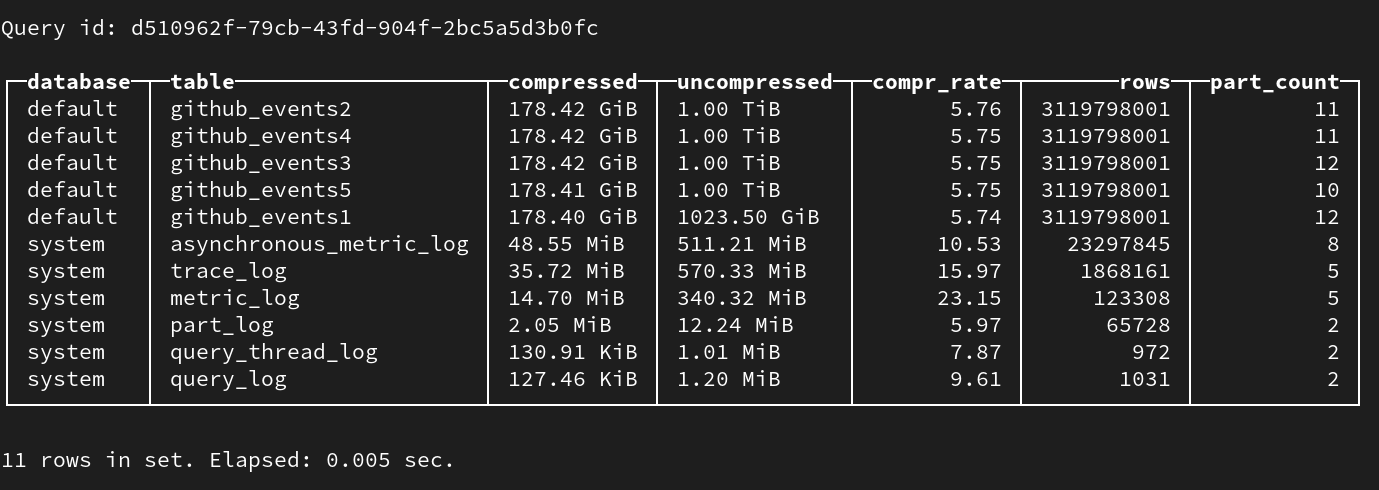
\includegraphics[width=.9\linewidth]{figures/clickhouse/table_size_local_backup.png}
\end{center}
\subsubsection{New attempt at downloading}
\label{sec:orgee99b19}
Delete local backup:
\begin{minted}[breaklines=true,breakanywhere=true]{bash}
./clickhouse-backup delete local 2022-05-11T07-25-16
# 2022/05/14 11:14:26.277665  info SELECT value FROM `system`.`build_options` where name='VERSION_INTEGER'
# 2022/05/14 11:14:26.280677  info SELECT * FROM system.disks;
# 2022/05/14 11:14:26.327285  info done                      backup=2022-05-11T07-25-16 duration=52ms location=local operation=delete
\end{minted}

List remote backups
\begin{minted}[breaklines=true,breakanywhere=true]{bash}
./clickhouse-backup list remote --config config.yaml
# 2022/05/14 11:15:16.688656  info SELECT max(toInt64(bytes_on_disk * 1.02)) AS max_file_size FROM system.parts
# 2022-05-11T07-25-16   895.29GiB   11/05/2022 10:44:05   remote      tar
# 2022-05-14T10-12-59   2.81KiB     14/05/2022 10:13:31   remote      tar
\end{minted}

Downloading the remote backup failed once again:
\begin{minted}[breaklines=true,breakanywhere=true]{bash}
time ./clickhouse-backup download 2022-05-11T07-25-16 --config config.yaml
# 2022/05/14 11:16:23.426432  info SELECT value FROM `system`.`build_options` where name='VERSION_INTEGER'
# 2022/05/14 11:16:23.428319  info SELECT * FROM system.disks;
# 2022/05/14 11:16:23.433846  info SELECT max(toInt64(bytes_on_disk * 1.02)) AS max_file_size FROM system.parts
# 2022/05/14 11:16:23.506743  info done                      backup=2022-05-11T07-25-16 duration=16ms operation=download size=3.36KiB table_metadata=default.github_events1
# 2022/05/14 11:16:23.512251  info done                      backup=2022-05-11T07-25-16 duration=5ms operation=download size=3.32KiB table_metadata=default.github_events2
# 2022/05/14 11:16:23.517891  info done                      backup=2022-05-11T07-25-16 duration=6ms operation=download size=3.36KiB table_metadata=default.github_events3
# 2022/05/14 11:16:23.522455  info done                      backup=2022-05-11T07-25-16 duration=5ms operation=download size=3.32KiB table_metadata=default.github_events4
# 2022/05/14 11:16:23.527403  info done                      backup=2022-05-11T07-25-16 duration=5ms operation=download size=3.28KiB table_metadata=default.github_events5
# 2022/05/14 11:17:23.532041 error can't acquire semaphore during downloadTableData: context canceled---------]  70.38% 59s
# 2022/05/14 11:17:23.697884 error can't acquire semaphore during Download: context canceled backup=2022-05-11T07-25-16 operation=download
# 2022/05/14 11:18:23.730339 error can't acquire semaphore during downloadTableData: context canceled---------]   9.31% 59s
# 2022/05/14 11:18:23.914406 error one of Download go-routine return error: one of downloadTableData go-routine return error: handling file: /all_3441_4218_4/push_distinct_size.bin: context deadline exceeded
#
# real    2m0.504s
# user    0m11.834s
# sys     0m16.363s
\end{minted}

 \section{Encrypt ClickHouse and recover from backup} \label{app:chs1e1}
In this experiment, we install \texttt{ccrypt} (an encryption tool)
in order to encrypt database files and observe the results.
Afterwards, we recover the VM using \texttt{clickhouse-backup} and Azure Backup respectively.
We attempted to encrypt a single file, as well as an entire directory.

This experiment has two main objectives.
One is to encrypt data files used by ClickHouse and observe the results.
How will database queries be affected?
Is it possible to detect a ransomware that encrypts ClickHouse's data files?
The other objective is to recover the database after the files have been encrypted.
The goal is to learn how to configure and use both \texttt{clickhouse-backup} and Azure Backup,
as well as evaluating their usability.

\subsection{Procedure}
\label{sec:org8373240}
Files were encrypted by using the tool \texttt{ccrypt}
with an empty passphrase (example: \texttt{ccrypt -e filename}).

SQL queries were run as \texttt{azureuser} (the default, non-root user) via \texttt{clickhouse-client}.

Bash commands were also run as \texttt{azureuser}.
Commands were run in \path{/home/azureuser} unless specified otherwise.

The output of commands and queries are shown in comments (\texttt{\#} for bash and PowerShell, \texttt{-{}-} for SQL) beneath the command or query.
Comments used to explain what a command does are placed above the command.
The variables from \ref{app:ch-non-perf} need to be declared in order for many commands to work.

\subsection{Determine which files to encrypt}
\label{sec:orge561d86}
Before we could encrypt files, we had to find out which files to encrypt.

In order to find out where table data is stored,
the path to the \texttt{cell\_towers} table was fetched from \texttt{system.parts},
which, as the name suggests, contains the parts of a database table
(when using the MergeTree database engine).
A descripton of \texttt{system.parts} can be found in the ClickHouse documentation.
\cite{noauthor_parts_nodate}
% [PartsClickHouseDocs] 

Query to fetch path of the \texttt{cell\_towers} table:
\begin{minted}[breaklines=true,breakanywhere=true]{sql}
SELECT
    table,
    disk_name,
    path
FROM system.parts
WHERE table = 'cell_towers'
FORMAT TabSeparated

-- cell_towers     default /var/lib/clickhouse/store/c28/c283470d-9ab3-4be8-bd81-132274c9f9b0/all_1_35_2/
-- cell_towers     default /var/lib/clickhouse/store/c28/c283470d-9ab3-4be8-bd81-132274c9f9b0/all_36_41_1/
-- cell_towers     default /var/lib/clickhouse/store/c28/c283470d-9ab3-4be8-bd81-132274c9f9b0/all_42_42_0/
\end{minted}

We navigated to the first path listed and printed the contents of the directory (performed as root):
\begin{minted}[breaklines=true,breakanywhere=true]{bash}
cd /var/lib/clickhouse/store/c28/c283470d-9ab3-4be8-bd81-132274c9f9b0/all_1_35_2/
ls

# area.bin            cell.mrk2        count.txt                      lat.mrk2  net.bin        range.bin     unit.mrk2
# area.mrk2           changeable.bin   created.bin                    lon.bin   net.mrk2       range.mrk2    updated.bin
# averageSignal.bin   changeable.mrk2  created.mrk2                   lon.mrk2  primary.idx    samples.bin   updated.mrk2
# averageSignal.mrk2  checksums.txt    default_compression_codec.txt  mcc.bin   radio.bin.cpt  samples.mrk2
# cell.bin            columns.txt      lat.bin                        mcc.mrk2  radio.mrk2     unit.bin
\end{minted}

In order to determine which files corresponded to columns in the table,
we used \texttt{DESCRIBE TABLE} to display the columns.

\begin{minted}[breaklines=true,breakanywhere=true]{sql}
DESCRIBE TABLE cell_towers
FORMAT TabSeparated

-- radio   Enum8(\'\' = 0, \'CDMA\' = 1, \'GSM\' = 2, \'LTE\' = 3, \'NR\' = 4, \'UMTS\' = 5)
-- mcc     UInt16
-- net     UInt16
-- area    UInt16
-- cell    UInt64
-- unit    Int16
-- lon     Float64
-- lat     Float64
-- range   UInt32
-- samples UInt32
-- changeable      UInt8
-- created DateTime
-- updated DateTime
-- averageSignal   UInt8
\end{minted}

Some of the column names displayed matched the names of files in the directory.
We made an educated guess that \texttt{.bin} files are the actual data files.
A quick Google search indicates that \texttt{.mrk2} files are related to the indexing of the database.

We decided to encrypt the file \texttt{radio.bin},
since the \texttt{radio} column is used in one of the test queries we will use.

\subsection{Install \texttt{ccrypt}}
\label{sec:orga964650}
\begin{minted}[breaklines=true,breakanywhere=true]{bash}
sudo apt install ccrypt
\end{minted}
\subsection{Perform test queries}
\label{sec:org0e389d8}
In order to see how encryption would affect the database,
we first performed two test queries and noted the results.
The queries are the same as the ones used in the \ref{app:ch-non-perf}.

Test query 1:
\begin{minted}[breaklines=true,breakanywhere=true]{sql}
SELECT
    radio,
    count() AS c
FROM cell_towers
GROUP BY radio
ORDER BY c DESC
FORMAT TabSeparated

-- UMTS 20686487
-- LTE  12101148
-- GSM  9931312
-- CDMA 556344
-- NR   867
\end{minted}

Test query 2:
\begin{minted}[breaklines=true,breakanywhere=true]{sql}
SELECT
    mcc,
    count()
FROM cell_towers
GROUP BY mcc
ORDER BY count() DESC
LIMIT 10
FORMAT TabSeparated

-- 310  5024650
-- 262  2622423
-- 250  1953176
-- 208  1891187
-- 724  1836150
-- 404  1729151
-- 234  1618924
-- 510  1353998
-- 440  1343355
-- 311  1332798
\end{minted}
\subsection{Encrypt file and repeat test queries}
\label{sec:orgec4825e}
Navigate to directory and encrypt \texttt{radio.bin} (performed as root):
\begin{minted}[breaklines=true,breakanywhere=true]{bash}
cd /var/lib/clickhouse/store/c28/c283470d-9ab3-4be8-bd81-132274c9f9b0/all_1_35_2
ccrypt -e radio.bin
\end{minted}

The test queries from earlier were repeated in \texttt{clickhouse-client}.
The first test query, which selects data from the \texttt{radio} table fails,
because the file \texttt{radio.bin}, which contains a part of the table used
for the query, is encrypted.

Query using \texttt{radio}, which fails because \texttt{radio.bin} is encrypted:
\begin{minted}[breaklines=true,breakanywhere=true]{sql}
SELECT
    radio,
    count() AS c
FROM cell_towers
GROUP BY radio
ORDER BY c DESC
FORMAT TabSeparated

-- Received exception from server (version 22.4.3):
-- Code: 107. DB::Exception: Received from localhost:9000. DB::Exception: Cannot open file /var/lib/clickhouse/store/c28/c283470d-9ab3-4be8-bd81-132274c9f9b0/all_1_35_2/radio.bin, errno: 2, strerror: No such file or directory: While executing MergeTreeInOrder. (FILE_DOESNT_EXIST)
\end{minted}

The other test query, which does not use the \texttt{radio} table succeeds:
\begin{minted}[breaklines=true,breakanywhere=true]{sql}
SELECT
    mcc,
    count()
FROM cell_towers
GROUP BY mcc
ORDER BY count() DESC
LIMIT 10
FORMAT TabSeparated

-- 310  5024650
-- 262  2622423
-- 250  1953176
-- 208  1891187
-- 724  1836150
-- 404  1729151
-- 234  1618924
-- 510  1353998
-- 440  1343355
-- 311  1332798
\end{minted}
\subsection{Decrypt file and repeat test query}
\label{sec:org164be71}
The file \texttt{radio.bin.cpt} (the encrypted version of \texttt{radio.bin}) was decrypted
with \texttt{ccrypt -d radio.bin.cpt},
and the test queries were repeated.
After decrypting the file, both queries succeeded.

First test query repeated after \texttt{radio.bin.cpt} was decrypted:
\begin{minted}[breaklines=true,breakanywhere=true]{sql}
SELECT
    radio,
    count() AS c
FROM cell_towers
GROUP BY radio
ORDER BY c DESC
FORMAT TabSeparated

-- UMTS 20686487
-- LTE  12101148
-- GSM  9931312
-- CDMA 556344
-- NR   867
\end{minted}

Second test query repeated after \texttt{radio.bin.cpt} was decrypted:
\begin{minted}[breaklines=true,breakanywhere=true]{sql}
SELECT
    mcc,
    count()
FROM cell_towers
GROUP BY mcc
ORDER BY count() DESC
LIMIT 10
FORMAT TabSeparated

-- 310 5024650
-- 262 2622423
-- 250 1953176
-- 208 1891187
-- 724 1836150
-- 404 1729151
-- 234 1618924
-- 510 1353998
-- 440 1343355
-- 311 1332798
\end{minted}

\subsection{Encrypt all files in \texttt{/var/lib/clickhouse/store} and repeat test queries}
\label{sec:orgb28ee20}
In order to simulate a ransomware attack
where the attacker doesn't encrypt specific files one-by-one,
but instead encrypts the entire data directory automatically,
we encrypted the directory which stores the data parts for (non-system) ClickHouse tables.

Files in the directory \path{/var/lib/clickhouse/store},
were encrypted recursively (\texttt{-r}) using \texttt{ccrypt}.
The \texttt{-f} (force) flag makes \texttt{ccrypt} encrypt write-protected files without asking for confirmation.

Encrypting \texttt{store} (performed as root):
\begin{minted}[breaklines=true,breakanywhere=true]{bash}
ccrypt -erf store

-- Enter encryption key:
-- Enter encryption key: (repeat)
-- ccrypt: store/063/0638116a-3105-483f-a2e5-55287d4eaa27/202204_2295_2350_15: No such file or directory
-- ccrypt: store/063/0638116a-3105-483f-a2e5-55287d4eaa27/202204_2355_2355_0: No such file or directory
-- ccrypt: store/063/0638116a-3105-483f-a2e5-55287d4eaa27/202204_2351_2351_0: No such file or directory
-- ccrypt: store/11f/11fafbd1-2c3f-4621-a574-b4f7b5594988/202204_2794_2794_0: No such file or directory
-- ccrypt: store/11f/11fafbd1-2c3f-4621-a574-b4f7b5594988/202204_2140_2793_477: No such file or directory
\end{minted}

The contents of one of the encryted directories (performed as root):
\begin{minted}[breaklines=true,breakanywhere=true]{bash}
ls -l /var/lib/clickhouse/store/c28/c283470d-9ab3-4be8-bd81-132274c9f9b0/all_1_35_2

# Result:
# total 918640
# -rw-r----- 1 clickhouse clickhouse  41208741 Apr 26 13:09 area.bin.cpt
# -rw-r----- 1 clickhouse clickhouse    107576 Apr 26 13:09 area.mrk2.cpt
# -rw-r----- 1 clickhouse clickhouse    163548 Apr 26 13:09 averageSignal.bin.cpt
# -rw-r----- 1 clickhouse clickhouse    107576 Apr 26 13:09 averageSignal.mrk2.cpt
# -rw-r----- 1 clickhouse clickhouse 157679630 Apr 26 13:09 cell.bin.cpt
# -rw-r----- 1 clickhouse clickhouse    107576 Apr 26 13:09 cell.mrk2.cpt
# -rw-r----- 1 clickhouse clickhouse    163548 Apr 26 13:09 changeable.bin.cpt
# -rw-r----- 1 clickhouse clickhouse    107576 Apr 26 13:09 changeable.mrk2.cpt
# -rw-r----- 1 clickhouse clickhouse      1183 Apr 26 13:09 checksums.txt.cpt
# -rw-r----- 1 clickhouse clickhouse       354 Apr 26 13:09 columns.txt.cpt
# -rw-r----- 1 clickhouse clickhouse        40 Apr 26 13:09 count.txt.cpt
# -rw-r----- 1 clickhouse clickhouse  65728056 Apr 26 13:09 created.bin.cpt
# -rw-r----- 1 clickhouse clickhouse    107576 Apr 26 13:09 created.mrk2.cpt
# -rw-r----- 1 clickhouse clickhouse        42 Apr 26 13:09 default_compression_codec.txt.cpt
# -rw-r----- 1 clickhouse clickhouse 224774675 Apr 26 13:09 lat.bin.cpt
# -rw-r----- 1 clickhouse clickhouse    107576 Apr 26 13:09 lat.mrk2.cpt
# -rw-r----- 1 clickhouse clickhouse 227815661 Apr 26 13:09 lon.bin.cpt
# -rw-r----- 1 clickhouse clickhouse    107576 Apr 26 13:09 lon.mrk2.cpt
# -rw-r----- 1 clickhouse clickhouse    331043 Apr 26 13:09 mcc.bin.cpt
# -rw-r----- 1 clickhouse clickhouse    107576 Apr 26 13:09 mcc.mrk2.cpt
# -rw-r----- 1 clickhouse clickhouse    345344 Apr 26 13:09 net.bin.cpt
# -rw-r----- 1 clickhouse clickhouse    107576 Apr 26 13:09 net.mrk2.cpt
# -rw-r----- 1 clickhouse clickhouse     40361 Apr 26 13:09 primary.idx.cpt
# -rw-r----- 1 clickhouse clickhouse    163563 Apr 26 13:09 radio.bin.cpt
# -rw-r----- 1 clickhouse clickhouse    107576 Apr 26 13:09 radio.mrk2.cpt
# -rw-r----- 1 clickhouse clickhouse  41566798 Apr 26 13:09 range.bin.cpt
# -rw-r----- 1 clickhouse clickhouse    107576 Apr 26 13:09 range.mrk2.cpt
# -rw-r----- 1 clickhouse clickhouse  66713118 Apr 26 13:09 samples.bin.cpt
# -rw-r----- 1 clickhouse clickhouse    107576 Apr 26 13:09 samples.mrk2.cpt
# -rw-r----- 1 clickhouse clickhouse   1331731 Apr 26 13:09 unit.bin.cpt
# -rw-r----- 1 clickhouse clickhouse    107576 Apr 26 13:09 unit.mrk2.cpt
# -rw-r----- 1 clickhouse clickhouse 110977534 Apr 26 13:09 updated.bin.cpt
# -rw-r----- 1 clickhouse clickhouse    107576 Apr 26 13:09 updated.mrk2.cpt
\end{minted}

Then the test queries were repeated.

Test query 1 fails:
\begin{minted}[breaklines=true,breakanywhere=true]{sql}
SELECT
    mcc,
    count()
FROM cell_towers
GROUP BY mcc
ORDER BY count() DESC
LIMIT 10
FORMAT TabSeparated

-- Query id: 6d32968b-85bb-4059-9119-ae76a84b8c13
--
-- 0 rows in set. Elapsed: 0.023 sec.
--
-- Received exception from server (version 22.4.3):
-- Code: 107. DB::Exception: Received from localhost:9000. DB::Exception: Cannot open file /var/lib/clickhouse/store/c28/c283470d-9ab3-4be8-bd81-132274c9f9b0/all_1_35_2/mcc.bin, errno: 2, strerror: No such file or directory: While executing MergeTreeInOrder. (FILE_DOESNT_EXIST)
\end{minted}

Test query 2 also fails:
\begin{minted}[breaklines=true,breakanywhere=true]{sql}
SELECT
    radio,
    count() AS c
FROM cell_towers
GROUP BY radio
ORDER BY c DESC
FORMAT TabSeparated

-- Query id: 8c913fd5-b0db-4cc2-b176-f389886c3bce
--
-- 0 rows in set. Elapsed: 0.003 sec.
--
-- Received exception from server (version 22.4.3):
-- Code: 107. DB::Exception: Received from localhost:9000. DB::Exception: Cannot open file /var/lib/clickhouse/store/c28/c283470d-9ab3-4be8-bd81-132274c9f9b0/all_1_35_2/radio.bin, errno: 2, strerror: No such file or directory: While executing MergeTreeInOrder. (FILE_DOESNT_EXIST)
\end{minted}

Selecting all columns fails:
\begin{minted}[breaklines=true,breakanywhere=true]{sql}
SELECT *
FROM cell_towers
LIMIT 10

-- Query id: 7a96d377-2f5b-4439-96d6-eb554b21fea7
--
-- 0 rows in set. Elapsed: 0.003 sec.
--
-- Received exception from server (version 22.4.3):
-- Code: 107. DB::Exception: Received from localhost:9000. DB::Exception: Cannot open file /var/lib/clickhouse/store/c28/c283470d-9ab3-4be8-bd81-132274c9f9b0/all_1_35_2/radio.bin, errno: 2, strerror: No such file or directory: While executing MergeTreeInOrder. (FILE_DOESNT_EXIST)
\end{minted}

Selecting any single column seems to fail:
\begin{minted}[breaklines=true,breakanywhere=true]{sql}
SELECT updated
FROM cell_towers
LIMIT 10

-- Query id: c983d27d-144d-4296-adb3-ade5ebba3777
--
--
-- 0 rows in set. Elapsed: 0.002 sec.
--
-- Received exception from server (version 22.4.3):
-- Code: 107. DB::Exception: Received from localhost:9000. DB::Exception: Cannot open file /var/lib/clickhouse/store/c28/c283470d-9ab3-4be8-bd81-132274c9f9b0/all_1_35_2/updated.bin, errno: 2, strerror: No such file or directory: While executing MergeTreeInOrder. (FILE_DOESNT_EXIST)
\end{minted}

\subsection{Rebuild VM and try to recover}
\label{sec:orgeb16138}
\subsubsection{Delete VM}
\label{sec:orga4a9443}
Script to delete the VM and accociated resources (run in Azure Cloud Shell):
\begin{minted}[breaklines=true,breakanywhere=true]{powershell}
# Delete the VM
az vm delete --name $CHName --resource-group $RGName --yes

# Get all resources in resource group
$resources = az resource list --resource-group $RGName | ConvertFrom-Json -AsHashtable

# Fetch only the ids of resources with names containing "clickhouse".
# The VM was named "clickhouseVM", which is why this works.
# If the VM had a different name, we would have to grep for something else.
$filtered = foreach($r in $resources) {
    Write-Output $r["id"] | grep clickhouse
}

# Delete the resources
$filtered | % {Remove-AzResource -ResourceId $_ -Force}
$filtered | % {Remove-AzResource -ResourceId $_ -Force}
\end{minted}

The last command had to be run twice,
because some resources could not be deleted while other resources depended on them.
Repeating the command had the effect of deleting ``child'' resources first,
so that ``parent'' resources could be deleted.

\subsubsection{Set up VM according to test environment setup}
\label{sec:orge14ae6f}
Outputs were skipped for the sake of brevity.
Everything went as planned.

Create VM (run from cloud shell):
\begin{minted}[breaklines=true,breakanywhere=true]{powershell}
az vm create `
    --resource-group $RGName `
    --name $CHName `
    --image Canonical:UbuntuServer:16.04-LTS:16.04.202109280 `
    --admin-username azureuser `
    --size Standard_B1s `
    --ssh-key-values $SSHPath `
    --public-ip-sku Standard
\end{minted}

Install clickhouse (run from bash in VM):
\begin{minted}[breaklines=true,breakanywhere=true]{bash}
sudo apt-get install -y apt-transport-https ca-certificates dirmngr
sudo apt-key adv --keyserver hkp://keyserver.ubuntu.com:80 --recv 8919F6BD2B48D754

echo "deb https://packages.clickhouse.com/deb stable main" | sudo tee \
    /etc/apt/sources.list.d/clickhouse.list
sudo apt-get update

sudo apt-get install -y clickhouse-server clickhouse-client

sudo service clickhouse-server start
\end{minted}

Install clickhouse-backup (run from bash in VM):
\begin{minted}[breaklines=true,breakanywhere=true]{bash}
# Download archive containing binary
wget https://github.com/AlexAkulov/clickhouse-backup/releases/download/v1.3.2/clickhouse-backup-linux-amd64.tar.gz

# Decompress archive
tar -zxvf clickhouse-backup-linux-amd64.tar.gz

# Move binary to home directory
mv build/linux/amd64/clickhouse-backup ~

# Cleanup
rmdir -p build/linux/amd64
rm clickhouse-backup-linux-amd64.tar.gz
\end{minted}

The \texttt{clickhouse-backup} config file was copied from
the test environment setup (see \ref{app:ch-non-perf})
and saved as \path{~/config.yaml}.

\subsubsection{Restore from remote backup}
\label{sec:org8a05b22}
Commands were run from bash on the VM.

List remote backups:
\begin{minted}[breaklines=true,breakanywhere=true]{bash}
sudo ./clickhouse-backup list remote --config config.yaml

# 2022/05/03 10:38:55.223041  info SELECT max(toInt64(bytes_on_disk * 1.02)) AS max_file_size FROM system.parts
# 2022-05-02T09-48-18   1.07GiB   02/05/2022 09:48:39   remote      tar
\end{minted}

Restore from the remote backup:
\begin{minted}[breaklines=true,breakanywhere=true]{bash}
sudo ./clickhouse-backup restore_remote 2022-05-02T09-48-18 --config config.yaml

# 2022/05/03 10:40:28.403253  info SELECT value FROM `system`.`build_options` where name='VERSION_INTEGER'
# 2022/05/03 10:40:28.407883  info SELECT * FROM system.disks;
# 2022/05/03 10:40:28.422520  info SELECT max(toInt64(bytes_on_disk * 1.02)) AS max_file_size FROM system.parts
# 2022/05/03 10:40:28.512501  info done                      backup=2022-05-02T09-48-18 duration=10ms operation=download size=765B table_metadata=default.cell_towers
# 2022/05/03 10:40:48.487522  info done                      diff_parts=0 duration=0s operation=downloadDiffParts===================================================================================================================] 100.00% 15s
# 2022/05/03 10:40:49.252289  info done                      backup=2022-05-02T09-48-18 duration=20.739s operation=download_data size=1.07GiB table=default.cell_towers
# 2022/05/03 10:40:49.269557  info done                      backup=2022-05-02T09-48-18 duration=20.855s operation=download size=1.07GiB
# 2022/05/03 10:40:49.326168  info SELECT value FROM `system`.`build_options` where name='VERSION_INTEGER'
# 2022/05/03 10:40:49.420143  info SELECT * FROM system.disks;
# 2022/05/03 10:40:49.429084  info CREATE DATABASE IF NOT EXISTS default
# ENGINE = Atomic
# 2022/05/03 10:40:49.437031  info SELECT engine FROM system.databases WHERE name = 'default'
# 2022/05/03 10:40:49.440420  info DROP TABLE IF EXISTS `default`.`cell_towers` NO DELAY
# 2022/05/03 10:40:49.444862  info CREATE DATABASE IF NOT EXISTS `default`
# 2022/05/03 10:40:49.448408  info CREATE TABLE default.cell_towers UUID 'f9b9b44f-3af6-4bf5-9458-9ef6a81a3519' (`radio` Enum8('' = 0, 'CDMA' = 1, 'GSM' = 2, 'LTE' = 3, 'NR' = 4, 'UMTS' = 5), `mcc` UInt16, `net` UInt16, `area` UInt16, `cell` UInt64, `unit` Int16, `lon` Float64, `lat` Float64, `range` UInt32, `samples` UInt32, `changeable` UInt8, `created` DateTime, `updated` DateTime, `averageSignal` UInt8) ENGINE = MergeTree ORDER BY (radio, mcc, net, created) SETTINGS index_granularity = 8192
# 2022/05/03 10:40:49.498743  info SELECT count() FROM system.settings WHERE name = 'show_table_uuid_in_table_create_query_if_not_nil'
# 2022/05/03 10:40:49.519183  info SELECT name FROM system.databases WHERE engine IN ('MySQL','PostgreSQL')
# 2022/05/03 10:40:49.533985  info
#                 SELECT
#                         countIf(name='data_path') is_data_path_present,
#                         countIf(name='data_paths') is_data_paths_present,
#                         countIf(name='uuid') is_uuid_present,
#                         countIf(name='create_table_query') is_create_table_query_present,
#                         countIf(name='total_bytes') is_total_bytes_present
#                 FROM system.columns WHERE database='system' AND table='tables'
#
# 2022/05/03 10:40:49.545657  info SELECT database, name, engine , data_paths , uuid , create_table_query , coalesce(total_bytes, 0) AS total_bytes   FROM system.tables WHERE is_temporary = 0 SETTINGS show_table_uuid_in_table_create_query_if_not_nil=1
# 2022/05/03 10:40:49.566479  info SELECT sum(bytes_on_disk) as size FROM system.parts WHERE database='default' AND table='cell_towers' GROUP BY database, table
# 2022/05/03 10:40:49.578319  info ALTER TABLE `default`.`cell_towers` ATTACH PART 'all_1_35_2'
# 2022/05/03 10:40:49.589570  info ALTER TABLE `default`.`cell_towers` ATTACH PART 'all_36_41_1'
# 2022/05/03 10:40:49.596540  info ALTER TABLE `default`.`cell_towers` ATTACH PART 'all_42_42_0'
# 2022/05/03 10:40:49.601181  info done                      backup=2022-05-02T09-48-18 operation=restore table=default.cell_towers
# 2022/05/03 10:40:49.601380  info done                      backup=2022-05-02T09-48-18 duration=109ms operation=restore
# 2022/05/03 10:40:49.601555  info done                      backup=2022-05-02T09-48-18 operation=restore
\end{minted}

\subsubsection{Repeat test queries}
\label{sec:org4f2f2e4}
Test queries were run from \texttt{clickhouse-backup}
and compared with earlier results to se if they were valid.
Both queries returned valid results, indicating that the recovery was successful.

At first, performance was very poor.
Sometimes the queries would time out because they took too long (more than 300 seconds).
After restarting the VM, queries were as fast as usual (0.072s and 0.2s respectively).

Test query 1:
\begin{minted}[breaklines=true,breakanywhere=true]{sql}
SELECT
    radio,
    count() AS c
FROM cell_towers
GROUP BY radio
ORDER BY c DESC
FORMAT TabSeparated

-- Query id: fea063fa-98e6-4a99-b373-4f51d99be3c1
--
-- UMTS    20686487
-- LTE     12101148
-- GSM     9931312
-- CDMA    556344
-- NR      867
\end{minted}

Test query 2:
\begin{minted}[breaklines=true,breakanywhere=true]{sql}
SELECT
    mcc,
    count()
FROM cell_towers
GROUP BY mcc
ORDER BY count() DESC
LIMIT 10
FORMAT TabSeparated

-- Query id: e4cd8484-7d4e-4e97-b78f-5373ed61c2b2
--
-- 310     5024650
-- 262     2622423
-- 250     1953176
-- 208     1891187
-- 724     1836150
-- 404     1729151
-- 234     1618924
-- 510     1353998
-- 440     1343355
-- 311     1332798
\end{minted}

\subsection{Repeat encryption and recover database with Azure Backup}
\label{sec:org2f39a38}
\subsubsection{Encrypt \texttt{store} directory}
\label{sec:org53cf4ea}
Run as root in bash on the VM:
\begin{minted}[breaklines=true,breakanywhere=true]{bash}
ccrypt -erf /var/lib/clickhouse/store
\end{minted}
\subsubsection{Delete VM}
\label{sec:org3c61e5e}
Deleting the VM:
\begin{minted}[breaklines=true,breakanywhere=true]{powershell}
az vm delete --name $CHName --resource-group $RGName --yes
\end{minted}

When using Azure Backup via the Azure Portal to recover a VM,
a virtual network and a subnet have to be provided.
We assume the same holds true for recovering via the Azure CLI,
even though no commands seem to be asking for the aforementioned resources (at least not directly).
This is why we only deleted the VM, and not related resources like network cards and IP adresses as well.

\subsubsection{Create a Storage Account}
\label{sec:orgab49f59}
In order to recover the VM, a storage account is required for staging the recovery.

Creating a storage account:
\begin{minted}[breaklines=true,breakanywhere=true]{powershell}
az storage account create `
    --name $StagingSAName `
    --resource-group $RGName `
    --location eastus `
    --sku Standard_LRS
\end{minted}

Output:
\begin{minted}[breaklines=true,breakanywhere=true]{json}
{
  "accessTier": "Hot",
  "allowBlobPublicAccess": true,
  "allowCrossTenantReplication": null,
  "allowSharedKeyAccess": null,
  "allowedCopyScope": null,
  "azureFilesIdentityBasedAuthentication": null,
  "blobRestoreStatus": null,
  "creationTime": "2022-05-04T07:11:01.403417+00:00",
  "customDomain": null,
  "defaultToOAuthAuthentication": null,
  "dnsEndpointType": null,
  "enableHttpsTrafficOnly": true,
  "enableNfsV3": null,
  "encryption": {
    "encryptionIdentity": null,
    "keySource": "Microsoft.Storage",
    "keyVaultProperties": null,
    "requireInfrastructureEncryption": null,
    "services": {
      "blob": {
        "enabled": true,
        "keyType": "Account",
        "lastEnabledTime": "2022-05-04T07:11:01.528489+00:00"
      },
      "file": {
        "enabled": true,
        "keyType": "Account",
        "lastEnabledTime": "2022-05-04T07:11:01.528489+00:00"
      },
      "queue": null,
      "table": null
    }
  },
  "extendedLocation": null,
  "failoverInProgress": null,
  "geoReplicationStats": null,
  "id": "/subscriptions/4b48eb85-91f3-4902-b74b-e84641fb6785/resourceGroups/testRG/providers/Microsoft.Storage/storageAccounts/stagingchsa",
  "identity": null,
  "immutableStorageWithVersioning": null,
  "isHnsEnabled": null,
  "isLocalUserEnabled": null,
  "isSftpEnabled": null,
  "keyCreationTime": {
    "key1": "2022-05-04T07:11:01.528489+00:00",
    "key2": "2022-05-04T07:11:01.528489+00:00"
  },
  "keyPolicy": null,
  "kind": "StorageV2",
  "largeFileSharesState": null,
  "lastGeoFailoverTime": null,
  "location": "eastus",
  "minimumTlsVersion": "TLS1_0",
  "name": "stagingchsa",
  "networkRuleSet": {
    "bypass": "AzureServices",
    "defaultAction": "Allow",
    "ipRules": [],
    "resourceAccessRules": null,
    "virtualNetworkRules": []
  },
  "primaryEndpoints": {
    "blob": "https://stagingchsa.blob.core.windows.net/",
    "dfs": "https://stagingchsa.dfs.core.windows.net/",
    "file": "https://stagingchsa.file.core.windows.net/",
    "internetEndpoints": null,
    "microsoftEndpoints": null,
    "queue": "https://stagingchsa.queue.core.windows.net/",
    "table": "https://stagingchsa.table.core.windows.net/",
    "web": "https://stagingchsa.z13.web.core.windows.net/"
  },
  "primaryLocation": "eastus",
  "privateEndpointConnections": [],
  "provisioningState": "Succeeded",
  "publicNetworkAccess": null,
  "resourceGroup": "testRG",
  "routingPreference": null,
  "sasPolicy": null,
  "secondaryEndpoints": null,
  "secondaryLocation": null,
  "sku": {
    "name": "Standard_LRS",
    "tier": "Standard"
  },
  "statusOfPrimary": "available",
  "statusOfSecondary": null,
  "storageAccountSkuConversionStatus": null,
  "tags": {},
  "type": "Microsoft.Storage/storageAccounts"
}
\end{minted}

\subsubsection{Recover from Azure Backup}
\label{sec:orgd58c2f9}
The VM was recovered by modifying instructions in the documentation \cite{v-amallick_back_nodate-1}
to suit our use case.
% [v-amallickBackRecoverAzure]
Many steps, like creating a Recovery Services vault, had already been performed and were thus skipped.
The commands we performed to recover the VM are listed below.
The process consists of retrieving information used to list relevant recovery points.
Then, a restore job is started in order to recover the VHD.
When the restore job is finished,
it produces a template which is then used to deploy a new VM.

Initial setup:
\begin{minted}[breaklines=true,breakanywhere=true]{powershell}
# Get RSV and set context
$RSV = Get-AzRecoveryServicesVault -Name $RSVName -ResourceGroupName $RGName
Set-AzRecoveryServicesVaultContext -Vault $RSV

# Select VM
$namedContainer = Get-AzRecoveryServicesBackupContainer  -ContainerType "AzureVM" -Status "Registered" -FriendlyName $CHName -VaultId $RSV.ID
$backupitem = Get-AzRecoveryServicesBackupItem -Container $namedContainer  -WorkloadType "AzureVM" -VaultId $RSV.ID

# Get start and end date
$startDate = (Get-Date).AddDays(-7)
$endDate = Get-Date

# Store recovery points in variable
$rp = Get-AzRecoveryServicesBackupRecoveryPoint -Item $backupitem -StartDate $startdate.ToUniversalTime() -EndDate $enddate.ToUniversalTime() -VaultId $RSV.ID
\end{minted}

Show contents of \texttt{rp}:
\begin{minted}[breaklines=true,breakanywhere=true]{powershell}
$rp

# RecoveryPointId    RecoveryPointType  RecoveryPointTime      ContainerName                        ContainerType
# ---------------    -----------------  -----------------      -------------                        -------------
# 201217219254041    CrashConsistent    5/4/2022 9:30:41 AM    iaasvmcontainerv2;testrg;clickhouse… AzureVM
# 208189198246820    CrashConsistent    5/2/2022 10:35:59 PM   iaasvmcontainerv2;testrg;clickhouse… AzureVM
# 210069911701143    CrashConsistent    5/2/2022 12:37:15 PM   iaasvmcontainerv2;testrg;clickhouse… AzureVM
\end{minted}

The recovery point \texttt{\$rp[1]} (208189198246820) is the one that was triggered manually earlier (see \ref{app:ch-non-perf}).
It was chosen to be used for recovery.

A restore job was started:
\begin{minted}[breaklines=true,breakanywhere=true]{powershell}
# Select recovery point
$RecPoint = $rp[1]

# Create a restore job for the backup item
$restorejob = Restore-AzRecoveryServicesBackupItem -RecoveryPoint $RecPoint -StorageAccountName $StagingSAName -StorageAccountResourceGroupName $RGName -TargetResourceGroupName $RGName -VaultId $RSV.ID

# Wait for the restore job to complete
Wait-AzRecoveryServicesBackupJob -Job $restorejob -Timeout 43200

# Get details of the restore job
$restorejob = Get-AzRecoveryServicesBackupJob -Job $restorejob -VaultId $RSV.ID
$details = Get-AzRecoveryServicesBackupJobDetail -Job $restorejob -VaultId $RSV.ID

# Print details
$details
# WorkloadName     Operation            Status               StartTime                 EndTime                   JobID
# ------------     ---------            ------               ---------                 -------                   -----
# clickhousevm     Restore              Completed            5/4/2022 9:30:38 AM       5/4/2022 9:51:17 AM       3019de90-58c6-4f40-9157-cd53c7546223
\end{minted}

We then declared some variables based on the details, to be used for future commands:
\begin{minted}[breaklines=true,breakanywhere=true]{powershell}
$properties = $details.properties
$storageAccountName = $properties["Target Storage Account Name"]
$containerName = $properties["Config Blob Container Name"]
$templateBlobURI = $properties["Template Blob Uri"]
\end{minted}

The contents of \texttt{\$properties}:
\begin{minted}[breaklines=true,breakanywhere=true]{text}
Key                         Value
---                         -----
Job Type                    Recover disks
Target VM Name              vmName
Target Storage Account Name stagingchsa
Recovery point time         5/2/2022 10:35:59 PM
Config Blob Name            config-clickhousevm-19ee2306-41c2-49bf-896f-40aa8172d2ea.json
Config Blob Container Name  clickhousevm-0edd1295169343bda63beb53c8781b85
Config Blob Uri             https://stagingchsa.blob.core.windows.net/clickhousevm-0edd1295169343bda63beb53c8781b85/config-clickhousevm-19ee2306-41c2-49bf-896f-40aa8172d2ea.j…
Target resource group       testRG
Template Blob Uri           https://stagingchsa.blob.core.windows.net/clickhousevm-0edd1295169343bda63beb53c8781b85/azuredeploy19ee2306-41c2-49bf-896f-40aa8172d2ea.json
\end{minted}

Deploying the VM from the template:
\begin{minted}[breaklines=true,breakanywhere=true]{powershell}
# Template name was copied from the "Template Blob Uri"
$templateName = "azuredeploy19ee2306-41c2-49bf-896f-40aa8172d2ea.json"

# Set the storage account
Set-AzCurrentStorageAccount -Name $storageAccountName -ResourceGroupName $RGName

# Generate SAS token
$templateBlobFullURI = New-AzStorageBlobSASToken -Container $containerName -Blob $templateName -Permission r -FullUri

# Deploy VM (VirtualMachineName had to be specified interactively)
New-AzResourceGroupDeployment -Name $CHName -ResourceGroupName $RGName -TemplateUri $templateBlobFullURI
\end{minted}

Output from the \texttt{New-AzResourceGroupDeployment} (The VirtualMachineName had to be supplied via user input, indentation was adjusted for readability):
\begin{minted}[breaklines=true,breakanywhere=true]{text}
cmdlet New-AzResourceGroupDeployment at command pipeline position 1
Supply values for the following parameters:
(Type !? for Help.)
VirtualMachineName: clickhouseVM

DeploymentName          : clickhouseVM
ResourceGroupName       : testRG
ProvisioningState       : Succeeded
Timestamp               : 5/4/2022 11:50:42 AM
Mode                    : Incremental
TemplateLink            :
Uri            : https://stagingchsa.blob.core.windows.net/clickhousevm-0edd1295169343bda63beb53c8781b85/azuredeploy19ee2306-41c2-49bf-896f-40aa8172d
2ea.json?sv=2021-04-10&se=2022-05-04T12%3A46%3A51Z&sr=b&sp=r&sig=Le%2BGX1JoU%2FSivJi9EpXyk0bPHAXxBsww%2BxY7SpGsP9k%3D
ContentVersion : 1.0.0.0
Parameters              :
Name                           Type                       Value
=============================  =========================  ==========
virtualMachineName             String                     "clickhouseVM"
virtualNetwork                 String                     "clickhouseVMVNET"
virtualNetworkResourceGroup    String                     "testRG"
subnet                         String                     "clickhouseVMSubnet"
osDiskName                     String                     "clickhouseVMOSDisk"
networkInterfacePrefixName     String                     "clickhouseVMRestoredNIC"
publicIpAddressName            String                     "clickhouseVMRestoredip"

Outputs                 :
DeploymentDebugLogLevel :
\end{minted}
\subsubsection{Repeat test queries}
\label{sec:org704b2f8}
The test queries were repeated in \texttt{clickhouse-client}.
Both were successful and reasonably fast.

Test query 1:
\begin{minted}[breaklines=true,breakanywhere=true]{sql}
SELECT
    radio,
    count() AS c
FROM cell_towers
GROUP BY radio
ORDER BY c DESC
FORMAT TabSeparated

-- Query id: fa3847f4-e564-4c8b-b2be-e85e2d4db87e
--
-- UMTS	20686487
-- LTE	12101148
-- GSM	9931312
-- CDMA	556344
-- NR	867
--
-- 5 rows in set. Elapsed: 0.094 sec. Processed 43.28 million rows, 43.28 MB (462.68 million rows/s., 462.68 MB/s.)
\end{minted}

Test query 2:
\begin{minted}[breaklines=true,breakanywhere=true]{sql}
SELECT
    mcc,
    count()
FROM cell_towers
GROUP BY mcc
ORDER BY count() DESC
LIMIT 10
FORMAT TabSeparated

-- Query id: f944c5ad-937c-45fa-a9f1-d173d12f7dbc
--
-- 310	5024650
-- 262	2622423
-- 250	1953176
-- 208	1891187
-- 724	1836150
-- 404	1729151
-- 234	1618924
-- 510	1353998
-- 440	1343355
-- 311	1332798
--
-- 10 rows in set. Elapsed: 0.392 sec. Processed 43.28 million rows, 86.55 MB (110.54 million rows/s., 221.07 MB/s.)
\end{minted}

 \section{Encrypt local backups}
\label{app:chs2e1}
In this experiment, we encrypted local backups made with \texttt{clickhouse-backup}
and observed the results.

\subsection{Create and encrypt a local backup}
\label{sec:orgccc578b}
A local backup was created:
\begin{minted}[breaklines=true,breakanywhere=true]{bash}
sudo ./clickhouse-backup create
# 2022/05/06 13:33:41.900950  info SELECT name, engine FROM system.databases WHERE name NOT IN ('system', 'INFORMATION_SCHEMA', 'information_schema')
# 2022/05/06 13:33:41.910260  info SHOW CREATE DATABASE `default`
# 2022/05/06 13:33:41.922356  info SELECT count() FROM system.settings WHERE name = 'show_table_uuid_in_table_create_query_if_not_nil'
# 2022/05/06 13:33:41.928718  info SELECT name FROM system.databases WHERE engine IN ('MySQL','PostgreSQL')
# 2022/05/06 13:33:41.934157  info
# 		SELECT
# 			countIf(name='data_path') is_data_path_present,
# 			countIf(name='data_paths') is_data_paths_present,
# 			countIf(name='uuid') is_uuid_present,
# 			countIf(name='create_table_query') is_create_table_query_present,
# 			countIf(name='total_bytes') is_total_bytes_present
# 		FROM system.columns WHERE database='system' AND table='tables'
#
# 2022/05/06 13:33:41.945031  info SELECT database, name, engine , data_paths , uuid , create_table_query , coalesce(total_bytes, 0) AS total_bytes   FROM system.tables WHERE is_temporary = 0 SETTINGS show_table_uuid_in_table_create_query_if_not_nil=1
# 2022/05/06 13:33:41.969735  info SELECT value FROM `system`.`build_options` where name='VERSION_INTEGER'
# 2022/05/06 13:33:41.975802  info SELECT * FROM system.disks;
# 2022/05/06 13:33:41.981654  info ALTER TABLE `default`.`cell_towers` FREEZE WITH NAME '46510daab8304f1bb845cc0a3378dc81';
# 2022/05/06 13:33:42.094131  info done                      backup=2022-05-06T13-33-41 operation=create table=default.cell_towers
# 2022/05/06 13:33:42.094551  info SELECT value FROM `system`.`build_options` where name='VERSION_DESCRIBE'
# 2022/05/06 13:33:42.103890  info done                      backup=2022-05-06T13-33-41 duration=206ms operation=create
\end{minted}

The \texttt{backup} directory was encrypted (as \texttt{root}) with an empty passphrase (output truncated):
\begin{minted}[breaklines=true,breakanywhere=true]{bash}
ccrypt -erf /var/lib/clickhouse/backup
# Enter encryption key:
# Enter encryption key: (repeat)
# ccrypt: warning: backup/2022-05-06T13-33-41/shadow/default/cell_towers/default/all_36_41_1/updated.mrk2 has 2 links
# ccrypt: warning: backup/2022-05-06T13-33-41/shadow/default/cell_towers/default/all_36_41_1/lon.bin has 2 links
# ccrypt: warning: backup/2022-05-06T13-33-41/shadow/default/cell_towers/default/all_36_41_1/checksums.txt has 2 links
# ccrypt: warning: backup/2022-05-06T13-33-41/shadow/default/cell_towers/default/all_36_41_1/default_compression_codec.txt has 2 links
# ccrypt: warning: backup/2022-05-06T13-33-41/shadow/default/cell_towers/default/all_36_41_1/radio.bin has 2 links
# ccrypt: warning: backup/2022-05-06T13-33-41/shadow/default/cell_towers/default/all_36_41_1/count.txt has 2 links
# ccrypt: warning: backup/2022-05-06T13-33-41/shadow/default/cell_towers/default/all_36_41_1/range.bin has 2 links
# ccrypt: warning: backup/2022-05-06T13-33-41/shadow/default/cell_towers/default/all_36_41_1/area.bin has 2 links
# ccrypt: warning: backup/2022-05-06T13-33-41/shadow/default/cell_towers/default/all_36_41_1/lon.mrk2 has 2 links
# ccrypt: warning: backup/2022-05-06T13-33-41/shadow/default/cell_towers/default/all_36_41_1/primary.idx has 2 links
# ccrypt: warning: backup/2022-05-06T13-33-41/shadow/default/cell_towers/default/all_36_41_1/mcc.mrk2 has 2 links
# ccrypt: warning: backup/2022-05-06T13-33-41/shadow/default/cell_towers/default/all_36_41_1/columns.txt has 2 links
# ccrypt: warning: backup/2022-05-06T13-33-41/shadow/default/cell_towers/default/all_36_41_1/created.bin has 2 links
\end{minted}

Listing backups via \texttt{clickhouse-backup}:
\begin{minted}[breaklines=true,breakanywhere=true]{bash}
./clickhouse-backup list
# 2022/05/06 13:39:10.487501  info SELECT value FROM `system`.`build_options` where name='VERSION_INTEGER'
# 2022/05/06 13:39:10.601852  info SELECT * FROM system.disks;
# 2022-05-06T13-33-41   ???   06/05/2022 13:37:27   local
\end{minted}

Trying to restore from the encrypted backup:
\begin{minted}[breaklines=true,breakanywhere=true]{bash}
./clickhouse-backup restore local 2022-05-06T13-33-41
# 2022/05/06 13:40:23.945646  info SELECT value FROM `system`.`build_options` where name='VERSION_INTEGER'
# 2022/05/06 13:40:23.950380  info SELECT * FROM system.disks;
# 2022/05/06 13:40:23.956845 error stat /var/lib/clickhouse/backup/local/metadata: no such file or directory
\end{minted}

We also discovered that the \texttt{clickhouse-client} would not start while \path{/var/lib/clickhouse/backup} was encrypted.

 \section{Delete backups via \texttt{clickhouse-backup}}
\label{app:chs2e2}
In this experiment, local and remote backups were deleted using \texttt{clickhouse-backup}.
Attempts were then made to recover the deleted remote files by undeleting them using the Azure CLI.
The first attempt failed, because soft delete had not been enabled correctly.
Soft delete was then enabled for blobs, and the experiment was repeated.

\subsection{Preparation}
\label{sec:orgde09cc4}
The following variables were declared:
\begin{minted}[breaklines=true,breakanywhere=true]{powershell}
$AccKey = "NdbW07WlHBf5zcpMXundwkP88Ie2SO1Ad+84VD8moaUg1ihIeRR7cEdy4FXIgHRvIQwPIMc7eD2q+ASt6EqxWg==" # Storage Account Access Key
$StorageAccount = Get-AzStorageAccount | Where-Object { $_.StorageAccountName -eq $SAName} # clickhouse-backup storage account
\end{minted}

\subsection{Delete local backups}
\label{sec:orgc3afe18}
Listing local backups:
\begin{minted}[breaklines=true,breakanywhere=true]{bash}
sudo ./clickhouse-backup list
# 2022/05/06 06:20:48.820972  info SELECT value FROM `system`.`build_options` where name='VERSION_INTEGER'
# 2022/05/06 06:20:48.830191  info SELECT * FROM system.disks;
# 2022-05-02T09-34-00   1.07GiB   02/05/2022 09:34:01   local
# 2022-05-02T09-48-03   1.07GiB   02/05/2022 09:48:03   local
# 2022-05-02T09-48-18   1.07GiB   02/05/2022 09:48:18   local
\end{minted}

Deleting all the local backups:
\begin{minted}[breaklines=true,breakanywhere=true]{bash}
sudo ./clickhouse-backup delete local 2022-05-02T09-34-00
# 2022/05/06 06:51:05.560887  info SELECT value FROM `system`.`build_options` where name='VERSION_INTEGER'
# 2022/05/06 06:51:05.567336  info SELECT * FROM system.disks;
# 2022/05/06 06:51:05.585788  info done                      backup=2022-05-02T09-34-00 duration=29ms location=local operation=delete

sudo ./clickhouse-backup delete local 2022-05-02T09-48-03
# 2022/05/06 06:51:05.630403  info SELECT value FROM `system`.`build_options` where name='VERSION_INTEGER'
# 2022/05/06 06:51:05.635599  info SELECT * FROM system.disks;
# 2022/05/06 06:51:05.645033  info done                      backup=2022-05-02T09-48-03 duration=18ms location=local operation=delete

sudo ./clickhouse-backup delete local 2022-05-02T09-48-18
# 2022/05/06 06:51:05.677436  info SELECT value FROM `system`.`build_options` where name='VERSION_INTEGER'
# 2022/05/06 06:51:05.683594  info SELECT * FROM system.disks;
# 2022/05/06 06:51:05.696499  info done                      backup=2022-05-02T09-48-18 duration=23ms location=local operation=delete
\end{minted}

Trying to list the backups (no results):
\begin{minted}[breaklines=true,breakanywhere=true]{bash}
sudo ./clickhouse-backup list
# 2022/05/06 06:52:09.307718  info SELECT value FROM `system`.`build_options` where name='VERSION_INTEGER'
# 2022/05/06 06:52:09.313018  info SELECT * FROM system.disks;
\end{minted}

\subsection{Delete remote backups via \texttt{clickhouse-backup} and restore via Azure CLI (first attempt)}
\label{sec:orgc78125c}
\subsubsection{Create remote backup}
\label{sec:orga0b4c06}
Creating a remote backup:
\begin{minted}[breaklines=true,breakanywhere=true]{bash}
sudo ./clickhouse-backup create_remote --config config.yaml
# 2022/05/06 12:08:24.906957  info SELECT name, engine FROM system.databases WHERE name NOT IN ('system', 'INFORMATION_SCHEMA', 'information_schema')
# 2022/05/06 12:08:24.916734  info SHOW CREATE DATABASE `default`
# 2022/05/06 12:08:24.928118  info SELECT count() FROM system.settings WHERE name = 'show_table_uuid_in_table_create_query_if_not_nil'
# 2022/05/06 12:08:24.934948  info SELECT name FROM system.databases WHERE engine IN ('MySQL','PostgreSQL')
# 2022/05/06 12:08:24.940334  info
# 		SELECT
# 			countIf(name='data_path') is_data_path_present,
# 			countIf(name='data_paths') is_data_paths_present,
# 			countIf(name='uuid') is_uuid_present,
# 			countIf(name='create_table_query') is_create_table_query_present,
# 			countIf(name='total_bytes') is_total_bytes_present
# 		FROM system.columns WHERE database='system' AND table='tables'
#
# 2022/05/06 12:08:24.947893  info SELECT database, name, engine , data_paths , uuid , create_table_query , coalesce(total_bytes, 0) AS total_bytes   FROM system.tables WHERE is_temporary = 0 SETTINGS show_table_uuid_in_table_create_query_if_not_nil=1
# 2022/05/06 12:08:24.984565  info SELECT value FROM `system`.`build_options` where name='VERSION_INTEGER'
# 2022/05/06 12:08:24.991468  info SELECT * FROM system.disks;
# 2022/05/06 12:08:24.996567  info ALTER TABLE `default`.`cell_towers` FREEZE WITH NAME '247d916bc61f4c05af26280ad8f3be9f';
# 2022/05/06 12:08:25.032979  info done                      backup=2022-05-06T12-08-24 operation=create table=default.cell_towers
# 2022/05/06 12:08:25.034527  info SELECT value FROM `system`.`build_options` where name='VERSION_DESCRIBE'
# 2022/05/06 12:08:25.041405  info done                      backup=2022-05-06T12-08-24 duration=142ms operation=create
# 2022/05/06 12:08:25.047661  info SELECT value FROM `system`.`build_options` where name='VERSION_INTEGER'
# 2022/05/06 12:08:25.051625  info SELECT * FROM system.disks;
# 2022/05/06 12:08:25.059594  info SELECT max(toInt64(bytes_on_disk * 1.02)) AS max_file_size FROM system.parts
# 2022/05/06 12:10:21.914725  info done                      backup=2022-05-06T12-08-24 duration=1m56.772s operation=upload size=1.07GiB table=default.cell_towers
# 2022/05/06 12:10:21.932113  info done                      backup=2022-05-06T12-08-24 duration=1m56.89s operation=upload size=1.07GiB
\end{minted}

Listing remote backups:
\begin{minted}[breaklines=true,breakanywhere=true]{bash}
sudo ./clickhouse-backup list remote --config config.yaml
# 2022/05/06 12:13:23.147970  info SELECT max(toInt64(bytes_on_disk * 1.02)) AS max_file_size FROM system.parts
# 2022-05-06T12-08-24   1.07GiB   06/05/2022 12:10:21   remote      tar
\end{minted}

\subsubsection{Delete remote backup}
\label{sec:orgc9798ca}
Deleting remote backups:
\begin{minted}[breaklines=true,breakanywhere=true]{bash}
sudo ./clickhouse-backup delete remote 2022-05-06T12-08-24 --config config.yaml
# 2022/05/06 12:15:02.656213  info SELECT max(toInt64(bytes_on_disk * 1.02)) AS max_file_size FROM system.parts
# 2022/05/06 12:15:02.777130  info done                      backup=2022-05-06T12-08-24 duration=124ms location=remote operation=delete
\end{minted}

Trying to list remote backups (no result):
\begin{minted}[breaklines=true,breakanywhere=true]{bash}
sudo ./clickhouse-backup list remote --config config.yaml
# 2022/05/06 12:15:19.106515  info SELECT max(toInt64(bytes_on_disk * 1.02)) AS max_file_size FROM system.parts
\end{minted}

\subsubsection{Undelete remote backups via Azure CLI}
\label{sec:orgba36207}
Trying to list remote backups (blobs) via the Azure Cloud Shell (including deleted blobs):
\begin{minted}[breaklines=true,breakanywhere=true]{powershell}
az storage blob list --account-name $SAName --container-name $ContainerName --account-key $AccKey --include d
\end{minted}

The result was an empty array (\texttt{[]}).
The container was still visible in the Azure Portal, though.

It appears that \texttt{clickhouse-backup} bypasses container soft delete in a sense,
by deleting the contents of the container, but not the container itself.
Thus, the container (and the backups) cannot be undeleted, since it was never deleted in the first place.
To verify this, the container was deleted via the Azure Portal and then undeleted.

\subsection{Enable soft delete for blobs}
\label{sec:org351b010}
Since the previous attempt at recovering remote \texttt{clickhouse-backups} via soft delete failed,
because we used the ``wrong'' type of soft delete, we decided to try again.
This time, we enabled soft delete for the blobs themselves.

Enable soft delete for Blobs:
\begin{minted}[breaklines=true,breakanywhere=true]{powershell}
az storage account blob-service-properties update --account-name $SAName `
    --resource-group $RGName `
    --enable-delete-retention true `
    --delete-retention-days 7
\end{minted}

\begin{minted}[breaklines=true,breakanywhere=true]{json}
{
  "automaticSnapshotPolicyEnabled": null,
  "changeFeed": null,
  "containerDeleteRetentionPolicy": {
    "allowPermanentDelete": null,
    "days": 7,
    "enabled": true
  },
  "cors": {
    "corsRules": []
  },
  "defaultServiceVersion": null,
  "deleteRetentionPolicy": {
    "allowPermanentDelete": null,
    "days": 7,
    "enabled": true
  },
  "id": "/subscriptions/4b48eb85-91f3-4902-b74b-e84641fb6785/resourceGroups/testRG/providers/Microsoft.Storage/storageAccounts/chbksa/blobServices/default",
  "isVersioningEnabled": null,
  "lastAccessTimeTrackingPolicy": null,
  "name": "default",
  "resourceGroup": "testRG",
  "restorePolicy": null,
  "sku": null,
  "type": "Microsoft.Storage/storageAccounts/blobServices"
}
\end{minted}

\subsection{Delete remote backups via \texttt{clickhouse-backup} and restore via Azure CLI (second attempt)}
\label{sec:orge96f96c}
\subsubsection{Create remote backup}
\label{sec:org237f76e}
A remote backup was created:
\begin{minted}[breaklines=true,breakanywhere=true]{bash}
sudo ./clickhouse-backup create_remote --config config.yaml
# 2022/05/06 12:41:19.110753  info SELECT name, engine FROM system.databases WHERE name NOT IN ('system', 'INFORMATION_SCHEMA', 'information_schema')
# 2022/05/06 12:41:19.185348  info SHOW CREATE DATABASE `default`
# 2022/05/06 12:41:19.192509  info SELECT count() FROM system.settings WHERE name = 'show_table_uuid_in_table_create_query_if_not_nil'
# 2022/05/06 12:41:19.199675  info SELECT name FROM system.databases WHERE engine IN ('MySQL','PostgreSQL')
# 2022/05/06 12:41:19.205297  info
# 		SELECT
# 			countIf(name='data_path') is_data_path_present,
# 			countIf(name='data_paths') is_data_paths_present,
# 			countIf(name='uuid') is_uuid_present,
# 			countIf(name='create_table_query') is_create_table_query_present,
# 			countIf(name='total_bytes') is_total_bytes_present
# 		FROM system.columns WHERE database='system' AND table='tables'
#
# 2022/05/06 12:41:19.212594  info SELECT database, name, engine , data_paths , uuid , create_table_query , coalesce(total_bytes, 0) AS total_bytes   FROM system.tables WHERE is_temporary = 0 SETTINGS show_table_uuid_in_table_create_query_if_not_nil=1
# 2022/05/06 12:41:19.231869  info SELECT value FROM `system`.`build_options` where name='VERSION_INTEGER'
# 2022/05/06 12:41:19.237796  info SELECT * FROM system.disks;
# 2022/05/06 12:41:19.243268  info ALTER TABLE `default`.`cell_towers` FREEZE WITH NAME '8fac6ff911f04cf68521c2d87f778dd7';
# 2022/05/06 12:41:19.320599  info done                      backup=2022-05-06T12-41-19 operation=create table=default.cell_towers
# 2022/05/06 12:41:19.321056  info SELECT value FROM `system`.`build_options` where name='VERSION_DESCRIBE'
# 2022/05/06 12:41:19.330933  info done                      backup=2022-05-06T12-41-19 duration=227ms operation=create
# 2022/05/06 12:41:19.338082  info SELECT value FROM `system`.`build_options` where name='VERSION_INTEGER'
# 2022/05/06 12:41:19.342402  info SELECT * FROM system.disks;
# 2022/05/06 12:41:19.350151  info SELECT max(toInt64(bytes_on_disk * 1.02)) AS max_file_size FROM system.parts
# 2022/05/06 12:41:40.804639  info done                      backup=2022-05-06T12-41-19 duration=21.379s operation=upload size=1.07GiB table=default.cell_towers
# 2022/05/06 12:41:40.822260  info done                      backup=2022-05-06T12-41-19 duration=21.491s operation=upload size=1.07GiB
\end{minted}

Listing the remote backup:
\begin{minted}[breaklines=true,breakanywhere=true]{bash}
sudo ./clickhouse-backup list remote --config config.yaml
# 2022/05/06 12:43:35.718005  info SELECT max(toInt64(bytes_on_disk * 1.02)) AS max_file_size FROM system.parts
# 2022-05-06T12-41-19   1.07GiB   06/05/2022 12:41:40   remote      tar
\end{minted}

\subsubsection{Delete remote backup}
\label{sec:org1dca49d}
Deleting the remote backup:
\begin{minted}[breaklines=true,breakanywhere=true]{bash}
sudo ./clickhouse-backup delete remote 2022-05-06T12-41-19 --config config.yaml
# 2022/05/06 12:44:26.871214  info SELECT max(toInt64(bytes_on_disk * 1.02)) AS max_file_size FROM system.parts
# 2022/05/06 12:44:26.977566  info done                      backup=2022-05-06T12-41-19 duration=110ms location=remote operation=delete
\end{minted}

Listing the remote backup (no result):
\begin{minted}[breaklines=true,breakanywhere=true]{bash}
sudo ./clickhouse-backup list remote --config config.yaml
# 2022/05/06 12:44:54.497519  info SELECT max(toInt64(bytes_on_disk * 1.02)) AS max_file_size FROM system.parts
\end{minted}

Listing the deleted blobs in the Azure CLI:
\begin{minted}[breaklines=true,breakanywhere=true]{powershell}
az storage blob list --account-name $SAName --container-name $ContainerName --account-key $AccKey --include d
\end{minted}

Output (notice that \texttt{deleted} is \texttt{true} for the blobs):
\begin{minted}[breaklines=true,breakanywhere=true]{json}
[
  {
    "container": "chbkcontainer",
    "content": "",
    "deleted": true,
    "encryptedMetadata": null,
    "encryptionKeySha256": null,
    "encryptionScope": null,
    "hasLegalHold": null,
    "hasVersionsOnly": null,
    "immutabilityPolicy": {
      "expiryTime": null,
      "policyMode": null
    },
    "isAppendBlobSealed": null,
    "isCurrentVersion": null,
    "lastAccessedOn": null,
    "metadata": {},
    "name": "https:/chbksa.blob.core.windows.net/chbkcontainer/2022-05-06T12-41-19/metadata.json",
    "objectReplicationDestinationPolicy": null,
    "objectReplicationSourceProperties": [],
    "properties": {
      "appendBlobCommittedBlockCount": null,
      "blobTier": "Hot",
      "blobTierChangeTime": null,
      "blobTierInferred": true,
      "blobType": "BlockBlob",
      "contentLength": 518,
      "contentRange": null,
      "contentSettings": {
        "cacheControl": null,
        "contentDisposition": null,
        "contentEncoding": null,
        "contentLanguage": null,
        "contentMd5": null,
        "contentType": "application/octet-stream"
      },
      "copy": {
        "completionTime": null,
        "destinationSnapshot": null,
        "id": null,
        "incrementalCopy": null,
        "progress": null,
        "source": null,
        "status": null,
        "statusDescription": null
      },
      "creationTime": "2022-05-06T12:41:40+00:00",
      "deletedTime": "2022-05-07T12:27:14+00:00",
      "etag": "0x8DA2F5DC4E522F7",
      "lastModified": "2022-05-06T12:41:40+00:00",
      "lease": {
        "duration": null,
        "state": null,
        "status": null
      },
      "pageBlobSequenceNumber": null,
      "pageRanges": null,
      "rehydrationStatus": null,
      "remainingRetentionDays": 6,
      "serverEncrypted": true
    },
    "rehydratePriority": null,
    "requestServerEncrypted": null,
    "snapshot": null,
    "tagCount": null,
    "tags": null,
    "versionId": null
  },
  {
    "container": "chbkcontainer",
    "content": "",
    "deleted": true,
    "encryptedMetadata": null,
    "encryptionKeySha256": null,
    "encryptionScope": null,
    "hasLegalHold": null,
    "hasVersionsOnly": null,
    "immutabilityPolicy": {
      "expiryTime": null,
      "policyMode": null
    },
    "isAppendBlobSealed": null,
    "isCurrentVersion": null,
    "lastAccessedOn": null,
    "metadata": {},
    "name": "https:/chbksa.blob.core.windows.net/chbkcontainer/2022-05-06T12-41-19/metadata/default/cell_towers.json",
    "objectReplicationDestinationPolicy": null,
    "objectReplicationSourceProperties": [],
    "properties": {
      "appendBlobCommittedBlockCount": null,
      "blobTier": "Hot",
      "blobTierChangeTime": null,
      "blobTierInferred": true,
      "blobType": "BlockBlob",
      "contentLength": 888,
      "contentRange": null,
      "contentSettings": {
        "cacheControl": null,
        "contentDisposition": null,
        "contentEncoding": null,
        "contentLanguage": null,
        "contentMd5": null,
        "contentType": "application/octet-stream"
      },
      "copy": {
        "completionTime": null,
        "destinationSnapshot": null,
        "id": null,
        "incrementalCopy": null,
        "progress": null,
        "source": null,
        "status": null,
        "statusDescription": null
      },
      "creationTime": "2022-05-06T12:41:40+00:00",
      "deletedTime": "2022-05-07T12:27:14+00:00",
      "etag": "0x8DA2F5DC4E23D31",
      "lastModified": "2022-05-06T12:41:40+00:00",
      "lease": {
        "duration": null,
        "state": null,
        "status": null
      },
      "pageBlobSequenceNumber": null,
      "pageRanges": null,
      "rehydrationStatus": null,
      "remainingRetentionDays": 6,
      "serverEncrypted": true
    },
    "rehydratePriority": null,
    "requestServerEncrypted": null,
    "snapshot": null,
    "tagCount": null,
    "tags": null,
    "versionId": null
  },
  {
    "container": "chbkcontainer",
    "content": "",
    "deleted": true,
    "encryptedMetadata": null,
    "encryptionKeySha256": null,
    "encryptionScope": null,
    "hasLegalHold": null,
    "hasVersionsOnly": null,
    "immutabilityPolicy": {
      "expiryTime": null,
      "policyMode": null
    },
    "isAppendBlobSealed": null,
    "isCurrentVersion": null,
    "lastAccessedOn": null,
    "metadata": {},
    "name": "https:/chbksa.blob.core.windows.net/chbkcontainer/2022-05-06T12-41-19/shadow/default/cell_towers/default_all_1_35_2.tar",
    "objectReplicationDestinationPolicy": null,
    "objectReplicationSourceProperties": [],
    "properties": {
      "appendBlobCommittedBlockCount": null,
      "blobTier": "Hot",
      "blobTierChangeTime": null,
      "blobTierInferred": true,
      "blobType": "BlockBlob",
      "contentLength": 940539392,
      "contentRange": null,
      "contentSettings": {
        "cacheControl": null,
        "contentDisposition": null,
        "contentEncoding": null,
        "contentLanguage": null,
        "contentMd5": null,
        "contentType": "application/octet-stream"
      },
      "copy": {
        "completionTime": null,
        "destinationSnapshot": null,
        "id": null,
        "incrementalCopy": null,
        "progress": null,
        "source": null,
        "status": null,
        "statusDescription": null
      },
      "creationTime": "2022-05-06T12:41:36+00:00",
      "deletedTime": "2022-05-07T12:27:14+00:00",
      "etag": "0x8DA2F5DC241DE8B",
      "lastModified": "2022-05-06T12:41:36+00:00",
      "lease": {
        "duration": null,
        "state": null,
        "status": null
      },
      "pageBlobSequenceNumber": null,
      "pageRanges": null,
      "rehydrationStatus": null,
      "remainingRetentionDays": 6,
      "serverEncrypted": true
    },
    "rehydratePriority": null,
    "requestServerEncrypted": null,
    "snapshot": null,
    "tagCount": null,
    "tags": null,
    "versionId": null
  },
  {
    "container": "chbkcontainer",
    "content": "",
    "deleted": true,
    "encryptedMetadata": null,
    "encryptionKeySha256": null,
    "encryptionScope": null,
    "hasLegalHold": null,
    "hasVersionsOnly": null,
    "immutabilityPolicy": {
      "expiryTime": null,
      "policyMode": null
    },
    "isAppendBlobSealed": null,
    "isCurrentVersion": null,
    "lastAccessedOn": null,
    "metadata": {},
    "name": "https:/chbksa.blob.core.windows.net/chbkcontainer/2022-05-06T12-41-19/shadow/default/cell_towers/default_all_36_41_1.tar",
    "objectReplicationDestinationPolicy": null,
    "objectReplicationSourceProperties": [],
    "properties": {
      "appendBlobCommittedBlockCount": null,
      "blobTier": "Hot",
      "blobTierChangeTime": null,
      "blobTierInferred": true,
      "blobType": "BlockBlob",
      "contentLength": 201757696,
      "contentRange": null,
      "contentSettings": {
        "cacheControl": null,
        "contentDisposition": null,
        "contentEncoding": null,
        "contentLanguage": null,
        "contentMd5": null,
        "contentType": "application/octet-stream"
      },
      "copy": {
        "completionTime": null,
        "destinationSnapshot": null,
        "id": null,
        "incrementalCopy": null,
        "progress": null,
        "source": null,
        "status": null,
        "statusDescription": null
      },
      "creationTime": "2022-05-06T12:41:40+00:00",
      "deletedTime": "2022-05-07T12:27:14+00:00",
      "etag": "0x8DA2F5DC4B0D44C",
      "lastModified": "2022-05-06T12:41:40+00:00",
      "lease": {
        "duration": null,
        "state": null,
        "status": null
      },
      "pageBlobSequenceNumber": null,
      "pageRanges": null,
      "rehydrationStatus": null,
      "remainingRetentionDays": 6,
      "serverEncrypted": true
    },
    "rehydratePriority": null,
    "requestServerEncrypted": null,
    "snapshot": null,
    "tagCount": null,
    "tags": null,
    "versionId": null
  },
  {
    "container": "chbkcontainer",
    "content": "",
    "deleted": true,
    "encryptedMetadata": null,
    "encryptionKeySha256": null,
    "encryptionScope": null,
    "hasLegalHold": null,
    "hasVersionsOnly": null,
    "immutabilityPolicy": {
      "expiryTime": null,
      "policyMode": null
    },
    "isAppendBlobSealed": null,
    "isCurrentVersion": null,
    "lastAccessedOn": null,
    "metadata": {},
    "name": "https:/chbksa.blob.core.windows.net/chbkcontainer/2022-05-06T12-41-19/shadow/default/cell_towers/default_all_42_42_0.tar",
    "objectReplicationDestinationPolicy": null,
    "objectReplicationSourceProperties": [],
    "properties": {
      "appendBlobCommittedBlockCount": null,
      "blobTier": "Hot",
      "blobTierChangeTime": null,
      "blobTierInferred": true,
      "blobType": "BlockBlob",
      "contentLength": 8671232,
      "contentRange": null,
      "contentSettings": {
        "cacheControl": null,
        "contentDisposition": null,
        "contentEncoding": null,
        "contentLanguage": null,
        "contentMd5": null,
        "contentType": "application/octet-stream"
      },
      "copy": {
        "completionTime": null,
        "destinationSnapshot": null,
        "id": null,
        "incrementalCopy": null,
        "progress": null,
        "source": null,
        "status": null,
        "statusDescription": null
      },
      "creationTime": "2022-05-06T12:41:40+00:00",
      "deletedTime": "2022-05-07T12:27:14+00:00",
      "etag": "0x8DA2F5DC4DEE251",
      "lastModified": "2022-05-06T12:41:40+00:00",
      "lease": {
        "duration": null,
        "state": null,
        "status": null
      },
      "pageBlobSequenceNumber": null,
      "pageRanges": null,
      "rehydrationStatus": null,
      "remainingRetentionDays": 6,
      "serverEncrypted": true
    },
    "rehydratePriority": null,
    "requestServerEncrypted": null,
    "snapshot": null,
    "tagCount": null,
    "tags": null,
    "versionId": null
  }
]
\end{minted}

\subsubsection{Undelete remote backups via Azure CLI}
\label{sec:org3630c7e}
Undeleting the deleted backups:
\begin{minted}[breaklines=true,breakanywhere=true]{powershell}
# List all blobs and retrieve deleted blobs from list
$Blobs = az storage blob list --account-name $SAName --container-name $ContainerName --account-key $AccKey --include d | ConvertFrom-Json -AsHashtable
$DeletedBlobs = $($Blobs | Where-Object { $_.deleted })

# Undelete deleted blobs
foreach($Blob in $DeletedBlobs) {
    az storage blob undelete --container-name $ContainerName --name $Blob.name --account-key $AccKey --account-name $SAName
}
\end{minted}

Output:
\begin{minted}[breaklines=true,breakanywhere=true]{json}
{
  "undeleted": null
}
{
  "undeleted": null
}
{
  "undeleted": null
}
{
  "undeleted": null
}
{
  "undeleted": null
}
\end{minted}

\subsubsection{Verify results}
\label{sec:org0597206}
Listing the Blobs in the Azure Cloud Shell:

\begin{minted}[breaklines=true,breakanywhere=true]{powershell}
az storage blob list --account-name $SAName --container-name $ContainerName --account-key $AccKey --include d
\end{minted}

Output (notice that \texttt{deleted} is \texttt{null}):
\begin{minted}[breaklines=true,breakanywhere=true]{json}
[
  {
    "container": "chbkcontainer",
    "content": "",
    "deleted": null,
    "encryptedMetadata": null,
    "encryptionKeySha256": null,
    "encryptionScope": null,
    "hasLegalHold": null,
    "hasVersionsOnly": null,
    "immutabilityPolicy": {
      "expiryTime": null,
      "policyMode": null
    },
    "isAppendBlobSealed": null,
    "isCurrentVersion": null,
    "lastAccessedOn": null,
    "metadata": {},
    "name": "https:/chbksa.blob.core.windows.net/chbkcontainer/2022-05-06T12-41-19/metadata.json",
    "objectReplicationDestinationPolicy": null,
    "objectReplicationSourceProperties": [],
    "properties": {
      "appendBlobCommittedBlockCount": null,
      "blobTier": "Hot",
      "blobTierChangeTime": null,
      "blobTierInferred": true,
      "blobType": "BlockBlob",
      "contentLength": 518,
      "contentRange": null,
      "contentSettings": {
        "cacheControl": null,
        "contentDisposition": null,
        "contentEncoding": null,
        "contentLanguage": null,
        "contentMd5": null,
        "contentType": "application/octet-stream"
      },
      "copy": {
        "completionTime": null,
        "destinationSnapshot": null,
        "id": null,
        "incrementalCopy": null,
        "progress": null,
        "source": null,
        "status": null,
        "statusDescription": null
      },
      "creationTime": "2022-05-06T12:41:40+00:00",
      "deletedTime": null,
      "etag": "0x8DA2F5DC4E522F7",
      "lastModified": "2022-05-06T12:41:40+00:00",
      "lease": {
        "duration": null,
        "state": "available",
        "status": "unlocked"
      },
      "pageBlobSequenceNumber": null,
      "pageRanges": null,
      "rehydrationStatus": null,
      "remainingRetentionDays": null,
      "serverEncrypted": true
    },
    "rehydratePriority": null,
    "requestServerEncrypted": null,
    "snapshot": null,
    "tagCount": null,
    "tags": null,
    "versionId": null
  },
  {
    "container": "chbkcontainer",
    "content": "",
    "deleted": null,
    "encryptedMetadata": null,
    "encryptionKeySha256": null,
    "encryptionScope": null,
    "hasLegalHold": null,
    "hasVersionsOnly": null,
    "immutabilityPolicy": {
      "expiryTime": null,
      "policyMode": null
    },
    "isAppendBlobSealed": null,
    "isCurrentVersion": null,
    "lastAccessedOn": null,
    "metadata": {},
    "name": "https:/chbksa.blob.core.windows.net/chbkcontainer/2022-05-06T12-41-19/metadata/default/cell_towers.json",
    "objectReplicationDestinationPolicy": null,
    "objectReplicationSourceProperties": [],
    "properties": {
      "appendBlobCommittedBlockCount": null,
      "blobTier": "Hot",
      "blobTierChangeTime": null,
      "blobTierInferred": true,
      "blobType": "BlockBlob",
      "contentLength": 888,
      "contentRange": null,
      "contentSettings": {
        "cacheControl": null,
        "contentDisposition": null,
        "contentEncoding": null,
        "contentLanguage": null,
        "contentMd5": null,
        "contentType": "application/octet-stream"
      },
      "copy": {
        "completionTime": null,
        "destinationSnapshot": null,
        "id": null,
        "incrementalCopy": null,
        "progress": null,
        "source": null,
        "status": null,
        "statusDescription": null
      },
      "creationTime": "2022-05-06T12:41:40+00:00",
      "deletedTime": null,
      "etag": "0x8DA2F5DC4E23D31",
      "lastModified": "2022-05-06T12:41:40+00:00",
      "lease": {
        "duration": null,
        "state": "available",
        "status": "unlocked"
      },
      "pageBlobSequenceNumber": null,
      "pageRanges": null,
      "rehydrationStatus": null,
      "remainingRetentionDays": null,
      "serverEncrypted": true
    },
    "rehydratePriority": null,
    "requestServerEncrypted": null,
    "snapshot": null,
    "tagCount": null,
    "tags": null,
    "versionId": null
  },
  {
    "container": "chbkcontainer",
    "content": "",
    "deleted": null,
    "encryptedMetadata": null,
    "encryptionKeySha256": null,
    "encryptionScope": null,
    "hasLegalHold": null,
    "hasVersionsOnly": null,
    "immutabilityPolicy": {
      "expiryTime": null,
      "policyMode": null
    },
    "isAppendBlobSealed": null,
    "isCurrentVersion": null,
    "lastAccessedOn": null,
    "metadata": {},
    "name": "https:/chbksa.blob.core.windows.net/chbkcontainer/2022-05-06T12-41-19/shadow/default/cell_towers/default_all_1_35_2.tar",
    "objectReplicationDestinationPolicy": null,
    "objectReplicationSourceProperties": [],
    "properties": {
      "appendBlobCommittedBlockCount": null,
      "blobTier": "Hot",
      "blobTierChangeTime": null,
      "blobTierInferred": true,
      "blobType": "BlockBlob",
      "contentLength": 940539392,
      "contentRange": null,
      "contentSettings": {
        "cacheControl": null,
        "contentDisposition": null,
        "contentEncoding": null,
        "contentLanguage": null,
        "contentMd5": null,
        "contentType": "application/octet-stream"
      },
      "copy": {
        "completionTime": null,
        "destinationSnapshot": null,
        "id": null,
        "incrementalCopy": null,
        "progress": null,
        "source": null,
        "status": null,
        "statusDescription": null
      },
      "creationTime": "2022-05-06T12:41:36+00:00",
      "deletedTime": null,
      "etag": "0x8DA2F5DC241DE8B",
      "lastModified": "2022-05-06T12:41:36+00:00",
      "lease": {
        "duration": null,
        "state": "available",
        "status": "unlocked"
      },
      "pageBlobSequenceNumber": null,
      "pageRanges": null,
      "rehydrationStatus": null,
      "remainingRetentionDays": null,
      "serverEncrypted": true
    },
    "rehydratePriority": null,
    "requestServerEncrypted": null,
    "snapshot": null,
    "tagCount": null,
    "tags": null,
    "versionId": null
  },
  {
    "container": "chbkcontainer",
    "content": "",
    "deleted": null,
    "encryptedMetadata": null,
    "encryptionKeySha256": null,
    "encryptionScope": null,
    "hasLegalHold": null,
    "hasVersionsOnly": null,
    "immutabilityPolicy": {
      "expiryTime": null,
      "policyMode": null
    },
    "isAppendBlobSealed": null,
    "isCurrentVersion": null,
    "lastAccessedOn": null,
    "metadata": {},
    "name": "https:/chbksa.blob.core.windows.net/chbkcontainer/2022-05-06T12-41-19/shadow/default/cell_towers/default_all_36_41_1.tar",
    "objectReplicationDestinationPolicy": null,
    "objectReplicationSourceProperties": [],
    "properties": {
      "appendBlobCommittedBlockCount": null,
      "blobTier": "Hot",
      "blobTierChangeTime": null,
      "blobTierInferred": true,
      "blobType": "BlockBlob",
      "contentLength": 201757696,
      "contentRange": null,
      "contentSettings": {
        "cacheControl": null,
        "contentDisposition": null,
        "contentEncoding": null,
        "contentLanguage": null,
        "contentMd5": null,
        "contentType": "application/octet-stream"
      },
      "copy": {
        "completionTime": null,
        "destinationSnapshot": null,
        "id": null,
        "incrementalCopy": null,
        "progress": null,
        "source": null,
        "status": null,
        "statusDescription": null
      },
      "creationTime": "2022-05-06T12:41:40+00:00",
      "deletedTime": null,
      "etag": "0x8DA2F5DC4B0D44C",
      "lastModified": "2022-05-06T12:41:40+00:00",
      "lease": {
        "duration": null,
        "state": "available",
        "status": "unlocked"
      },
      "pageBlobSequenceNumber": null,
      "pageRanges": null,
      "rehydrationStatus": null,
      "remainingRetentionDays": null,
      "serverEncrypted": true
    },
    "rehydratePriority": null,
    "requestServerEncrypted": null,
    "snapshot": null,
    "tagCount": null,
    "tags": null,
    "versionId": null
  },
  {
    "container": "chbkcontainer",
    "content": "",
    "deleted": null,
    "encryptedMetadata": null,
    "encryptionKeySha256": null,
    "encryptionScope": null,
    "hasLegalHold": null,
    "hasVersionsOnly": null,
    "immutabilityPolicy": {
      "expiryTime": null,
      "policyMode": null
    },
    "isAppendBlobSealed": null,
    "isCurrentVersion": null,
    "lastAccessedOn": null,
    "metadata": {},
    "name": "https:/chbksa.blob.core.windows.net/chbkcontainer/2022-05-06T12-41-19/shadow/default/cell_towers/default_all_42_42_0.tar",
    "objectReplicationDestinationPolicy": null,
    "objectReplicationSourceProperties": [],
    "properties": {
      "appendBlobCommittedBlockCount": null,
      "blobTier": "Hot",
      "blobTierChangeTime": null,
      "blobTierInferred": true,
      "blobType": "BlockBlob",
      "contentLength": 8671232,
      "contentRange": null,
      "contentSettings": {
        "cacheControl": null,
        "contentDisposition": null,
        "contentEncoding": null,
        "contentLanguage": null,
        "contentMd5": null,
        "contentType": "application/octet-stream"
      },
      "copy": {
        "completionTime": null,
        "destinationSnapshot": null,
        "id": null,
        "incrementalCopy": null,
        "progress": null,
        "source": null,
        "status": null,
        "statusDescription": null
      },
      "creationTime": "2022-05-06T12:41:40+00:00",
      "deletedTime": null,
      "etag": "0x8DA2F5DC4DEE251",
      "lastModified": "2022-05-06T12:41:40+00:00",
      "lease": {
        "duration": null,
        "state": "available",
        "status": "unlocked"
      },
      "pageBlobSequenceNumber": null,
      "pageRanges": null,
      "rehydrationStatus": null,
      "remainingRetentionDays": null,
      "serverEncrypted": true
    },
    "rehydratePriority": null,
    "requestServerEncrypted": null,
    "snapshot": null,
    "tagCount": null,
    "tags": null,
    "versionId": null
  }
]
\end{minted}

Listing undeleted Blobs in \texttt{clickhouse-backup}:
\begin{minted}[breaklines=true,breakanywhere=true]{bash}
sudo ./clickhouse-backup list remote --config config.yaml
# 2022/05/07 12:26:27.136458  info SELECT max(toInt64(bytes_on_disk * 1.02)) AS max_file_size FROM system.parts
# 2022-05-06T12-41-19   1.07GiB   06/05/2022 12:41:40   remote      tar
\end{minted}

Restoring the database from the undeleted remote backup:
\begin{minted}[breaklines=true,breakanywhere=true]{bash}
sudo ./clickhouse-backup restore_remote 2022-05-06T12-41-19 --config config.yaml
# 2022/05/07 12:30:32.003711  info SELECT value FROM `system`.`build_options` where name='VERSION_INTEGER'
# 2022/05/07 12:30:32.007101  info SELECT * FROM system.disks;
# 2022/05/07 12:30:32.018499  info SELECT max(toInt64(bytes_on_disk * 1.02)) AS max_file_size FROM system.parts
# 2022/05/07 12:30:32.094614  info done                      backup=2022-05-06T12-41-19 duration=7ms operation=download size=765B table_metadata=default.cell_towers
# 2022/05/07 12:30:51.137543  info done                      diff_parts=0 duration=0s operation=downloadDiffParts100.00% 0s
# 2022/05/07 12:30:51.137700  info done                      backup=2022-05-06T12-41-19 duration=19.043s operation=download_data size=1.07GiB table=default.cell_towers
# 2022/05/07 12:30:51.146800  info done                      backup=2022-05-06T12-41-19 duration=19.135s operation=download size=1.07GiB
# 2022/05/07 12:30:52.193726  info SELECT value FROM `system`.`build_options` where name='VERSION_INTEGER'
# 2022/05/07 12:30:53.438041  info SELECT * FROM system.disks;
# 2022/05/07 12:30:53.441231  info CREATE DATABASE IF NOT EXISTS default
# ENGINE = Atomic
# 2022/05/07 12:30:53.458792  info SELECT engine FROM system.databases WHERE name = 'default'
# 2022/05/07 12:30:53.483831  info DROP TABLE IF EXISTS `default`.`cell_towers` NO DELAY
# 2022/05/07 12:30:53.509936  info CREATE DATABASE IF NOT EXISTS `default`
# 2022/05/07 12:30:53.517094  info CREATE TABLE default.cell_towers UUID 'f9b9b44f-3af6-4bf5-9458-9ef6a81a3519' (`radio` Enum8('' = 0, 'CDMA' = 1, 'GSM' = 2, 'LTE' = 3, 'NR' = 4, 'UMTS' = 5), `mcc` UInt16, `net` UInt16, `area` UInt16, `cell` UInt64, `unit` Int16, `lon` Float64, `lat` Float64, `range` UInt32, `samples` UInt32, `changeable` UInt8, `created` DateTime, `updated` DateTime, `averageSignal` UInt8) ENGINE = MergeTree ORDER BY (radio, mcc, net, created) SETTINGS index_granularity = 8192
# 2022/05/07 12:30:53.764502  info SELECT count() FROM system.settings WHERE name = 'show_table_uuid_in_table_create_query_if_not_nil'
# 2022/05/07 12:30:53.771475  info SELECT name FROM system.databases WHERE engine IN ('MySQL','PostgreSQL')
# 2022/05/07 12:30:53.780565  info
# 		SELECT
# 			countIf(name='data_path') is_data_path_present,
# 			countIf(name='data_paths') is_data_paths_present,
# 			countIf(name='uuid') is_uuid_present,
# 			countIf(name='create_table_query') is_create_table_query_present,
# 			countIf(name='total_bytes') is_total_bytes_present
# 		FROM system.columns WHERE database='system' AND table='tables'
#
# 2022/05/07 12:30:53.791797  info SELECT database, name, engine , data_paths , uuid , create_table_query , coalesce(total_bytes, 0) AS total_bytes   FROM system.tables WHERE is_temporary = 0 SETTINGS show_table_uuid_in_table_create_query_if_not_nil=1
# 2022/05/07 12:30:53.816765  info SELECT sum(bytes_on_disk) as size FROM system.parts WHERE database='default' AND table='cell_towers' GROUP BY database, table
# 2022/05/07 12:30:53.832002  info ALTER TABLE `default`.`cell_towers` ATTACH PART 'all_1_35_2'
# 2022/05/07 12:30:53.844536  info ALTER TABLE `default`.`cell_towers` ATTACH PART 'all_36_41_1'
# 2022/05/07 12:30:53.849068  info ALTER TABLE `default`.`cell_towers` ATTACH PART 'all_42_42_0'
# 2022/05/07 12:30:53.852548  info done                      backup=2022-05-06T12-41-19 operation=restore table=default.cell_towers
# 2022/05/07 12:30:53.852691  info done                      backup=2022-05-06T12-41-19 duration=94ms operation=restore
# 2022/05/07 12:30:53.852822  info done                      backup=2022-05-06T12-41-19 operation=restore
\end{minted}

The test queries were repeated in \texttt{clickhouse-client}.
The queries were hanging at first, so the VM was restarted.
Both were successful.

Test query 1:
\begin{minted}[breaklines=true,breakanywhere=true]{sql}
SELECT
    radio,
    count() AS c
FROM cell_towers
GROUP BY radio
ORDER BY c DESC
FORMAT TabSeparated

-- Query id: 4d363e44-943b-47c0-b926-abd323e4dd59
--
-- UMTS	20686487
-- LTE	12101148
-- GSM	9931312
-- CDMA	556344
-- NR	867
--
-- 5 rows in set. Elapsed: 0.055 sec. Processed 43.28 million rows, 43.28 MB (781.15 million rows/s., 781.15 MB/s.)
\end{minted}

Test query 2:
\begin{minted}[breaklines=true,breakanywhere=true]{sql}
SELECT
    mcc,
    count()
FROM cell_towers
GROUP BY mcc
ORDER BY count() DESC
LIMIT 10
FORMAT TabSeparated

-- Query id: ca9261f1-bb07-44f1-b83d-c95aab614203
--
-- 310	5024650
-- 262	2622423
-- 250	1953176
-- 208	1891187
-- 724	1836150
-- 404	1729151
-- 234	1618924
-- 510	1353998
-- 440	1343355
-- 311	1332798
--
-- 10 rows in set. Elapsed: 0.197 sec. Processed 43.28 million rows, 86.55 MB (220.03 million rows/s., 440.05 MB/s.)
\end{minted}

 \section{Delete backups stored in Azure blob storage via Azure CLI}
\label{app:chs2e3}
This experiment is similar to the previous one (\ref{app:chs2e2}),
except that the blobs were deleted via the Azure CLI,
instead of using \texttt{clickhouse-backup}.
Afterwards, the Blobs were restored.

\subsection{Preparation}
\label{sec:org4d48e1c}
The following variables were declared:
\begin{minted}[breaklines=true,breakanywhere=true]{powershell}
$AccKey = "NdbW07WlHBf5zcpMXundwkP88Ie2SO1Ad+84VD8moaUg1ihIeRR7cEdy4FXIgHRvIQwPIMc7eD2q+ASt6EqxWg==" # Storage Account Access Key
$StorageAccount = Get-AzStorageAccount | Where-Object { $_.StorageAccountName -eq $SAName} # clickhouse-backup storage account
\end{minted}

\subsection{Delete the blobs}
\label{sec:orge72cc5d}
Listing the blobs in Azure Cloud Shell:
\begin{minted}[breaklines=true,breakanywhere=true]{powershell}
az storage blob list --account-name $SAName --container-name $ContainerName --account-key $AccKey | ConvertFrom-Json -AsHashtable | % {$_.name}
# https:/chbksa.blob.core.windows.net/chbkcontainer/2022-05-06T12-41-19/metadata.json
# https:/chbksa.blob.core.windows.net/chbkcontainer/2022-05-06T12-41-19/metadata/default/cell_towers.json
# https:/chbksa.blob.core.windows.net/chbkcontainer/2022-05-06T12-41-19/shadow/default/cell_towers/default_all_1_35_2.tar
# https:/chbksa.blob.core.windows.net/chbkcontainer/2022-05-06T12-41-19/shadow/default/cell_towers/default_all_36_41_1.tar
# https:/chbksa.blob.core.windows.net/chbkcontainer/2022-05-06T12-41-19/shadow/default/cell_towers/default_all_42_42_0.tar
\end{minted}

Deleting the blobs:
\begin{minted}[breaklines=true,breakanywhere=true]{powershell}
# Store the list of blob names in a variable
$BlobNames = az storage blob list --account-name $SAName --container-name $ContainerName --account-key $AccKey | ConvertFrom-Json -AsHashtable | % {$_.name}

foreach($name in $BlobNames) {
    echo "Deleting $name"
    az storage blob delete --account-name $SAName --account-key $AccKey --container-name $ContainerName --name $name
}
# Deleting https:/chbksa.blob.core.windows.net/chbkcontainer/2022-05-06T12-41-19/metadata.json
# Deleting https:/chbksa.blob.core.windows.net/chbkcontainer/2022-05-06T12-41-19/metadata/default/cell_towers.json
# Deleting https:/chbksa.blob.core.windows.net/chbkcontainer/2022-05-06T12-41-19/shadow/default/cell_towers/default_all_1_35_2.tar
# Deleting https:/chbksa.blob.core.windows.net/chbkcontainer/2022-05-06T12-41-19/shadow/default/cell_towers/default_all_36_41_1.tar
# Deleting https:/chbksa.blob.core.windows.net/chbkcontainer/2022-05-06T12-41-19/shadow/default/cell_towers/default_all_42_42_0.tar
\end{minted}

After this, the blobs were no longer visible in the Azure portal (unless ``Show deleted blobs'' was enabled).
We decided to also verify this via \texttt{clickhouse-backup}.

Trying to list the blobs via \texttt{clickhouse-backup} (no result):
\begin{minted}[breaklines=true,breakanywhere=true]{bash}
sudo ./clickhouse-backup list remote --config config.yaml
# 2022/05/07 12:54:09.423781  info SELECT max(toInt64(bytes_on_disk * 1.02)) AS max_file_size FROM system.parts
\end{minted}

\subsection{Restore the blobs}
\label{sec:org9a5b383}
The process for restoring blobs is the same as in section \ref{sec:org3630c7e}.

Script to undelete deleted blobs:
\begin{minted}[breaklines=true,breakanywhere=true]{powershell}
# List all blobs and retrieve deleted blobs from list
$Blobs = az storage blob list --account-name $SAName --container-name $ContainerName --account-key $AccKey --include d | ConvertFrom-Json -AsHashtable
$DeletedBlobs = $($Blobs | Where-Object { $_.deleted })

# Undelete deleted blobs
foreach($Blob in $DeletedBlobs) {
    az storage blob undelete --container-name $ContainerName --name $Blob.name --account-key $AccKey --account-name $SAName
}
\end{minted}

Listing the blobs:
\begin{minted}[breaklines=true,breakanywhere=true]{powershell}
az storage blob list --account-name $SAName --container-name $ContainerName --account-key $AccKey | ConvertFrom-Json -AsHashtable | % {$_.name}
# https:/chbksa.blob.core.windows.net/chbkcontainer/2022-05-06T12-41-19/metadata.json
# https:/chbksa.blob.core.windows.net/chbkcontainer/2022-05-06T12-41-19/metadata/default/cell_towers.json
# https:/chbksa.blob.core.windows.net/chbkcontainer/2022-05-06T12-41-19/shadow/default/cell_towers/default_all_1_35_2.tar
# https:/chbksa.blob.core.windows.net/chbkcontainer/2022-05-06T12-41-19/shadow/default/cell_towers/default_all_36_41_1.tar
# https:/chbksa.blob.core.windows.net/chbkcontainer/2022-05-06T12-41-19/shadow/default/cell_towers/default_all_42_42_0.tar
\end{minted}

 \section{Delete backups in Azure Backup}
\label{app:chs2e4}
In this experiment,
backups were stopped for the ClickHouse VM,
and the backups were deleted.
Then the backups were restored from their soft deleted state,
and the backups were resumed.

\subsection{Delete Azure Backups via CLI}
\label{sec:org19b15b2}
Get the IDs of all backup items:
\begin{minted}[breaklines=true,breakanywhere=true]{powershell}
$itemIds = az backup item list --resource-group $RGName --vault-name $RSVName | ConvertFrom-Json -AsHashtable | % {$_["id"]}
\end{minted}

Disable protection for and delete all backup items:
\begin{minted}[breaklines=true,breakanywhere=true]{powershell}
foreach($id in $itemIds) {
    az backup protection disable --backup-management-type AzureIaasVM --delete-backup-data true --ids $id
}
\end{minted}

Output:
\begin{minted}[breaklines=true,breakanywhere=true]{json}
Are you sure you want to perform this operation? (y/n): y
{
  "eTag": null,
  "id": "/subscriptions/4b48eb85-91f3-4902-b74b-e84641fb6785/resourceGroups/testRG/providers/Microsoft.RecoveryServices/vaults/myRSV/backupJobs/bd6f9157-f5d1-4f67-9435-69737c6ab221",
  "location": null,
  "name": "bd6f9157-f5d1-4f67-9435-69737c6ab221",
  "properties": {
    "actionsInfo": null,
    "activityId": "4054af82-cd28-11ec-8904-0a580af40e30",
    "backupManagementType": "AzureIaasVM",
    "containerName": "iaasvmcontainerv2;testrg;clickhousevm",
    "duration": "0:00:11.138772",
    "endTime": "2022-05-06T10:35:45.276307+00:00",
    "entityFriendlyName": "clickhouseVM",
    "errorDetails": null,
    "extendedInfo": {
      "dynamicErrorMessage": null,
      "estimatedRemainingDuration": null,
      "internalPropertyBag": null,
      "progressPercentage": null,
      "propertyBag": {
        "Number of Recovery Points": "4",
        "VM Name": "clickhouseVM"
      },
      "tasksList": []
    },
    "isUserTriggered": null,
    "jobType": "AzureIaaSVMJob",
    "operation": "DeleteBackupData",
    "startTime": "2022-05-06T10:35:34.137536+00:00",
    "status": "Completed",
    "virtualMachineVersion": "Compute"
  },
  "resourceGroup": "testRG",
  "tags": null,
  "type": "Microsoft.RecoveryServices/vaults/backupJobs"
}
\end{minted}

This triggered an alert from Azure Monitor (``Delete Backup Data'' alert).

Listing the backup items:
\begin{minted}[breaklines=true,breakanywhere=true]{powershell}
az backup item list --resource-group $RGName --vault-name $RSVName
\end{minted}

Output:
\begin{minted}[breaklines=true,breakanywhere=true]{json}
[
  {
    "eTag": null,
    "id": "/subscriptions/4b48eb85-91f3-4902-b74b-e84641fb6785/resourceGroups/testRG/providers/Microsoft.RecoveryServices/vaults/myRSV/backupFabrics/Azure/protectionContainers/IaasVMContainer;iaasvmcontainerv2;testrg;clickhousevm/protectedItems/VM;iaasvmcontainerv2;testrg;clickhousevm",
    "location": null,
    "name": "VM;iaasvmcontainerv2;testrg;clickhousevm",
    "properties": {
      "backupManagementType": "AzureIaasVM",
      "backupSetName": null,
      "containerName": "iaasvmcontainerv2;testrg;clickhousevm",
      "createMode": null,
      "deferredDeleteTimeInUtc": "2022-05-06T10:35:34.137536+00:00",
      "deferredDeleteTimeRemaining": "13.23:48:44.6226505",
      "extendedInfo": null,
      "extendedProperties": {
        "diskExclusionProperties": null,
        "linuxVmApplicationName": ""
      },
      "friendlyName": "clickhouseVM",
      "healthDetails": [
        {
          "code": 400239,
          "message": "Backup pre-check status of this virtual machine is OK.",
          "recommendations": [],
          "title": "IaasVmHealthGreenDefault"
        }
      ],
      "healthStatus": "Passed",
      "isArchiveEnabled": false,
      "isDeferredDeleteScheduleUpcoming": null,
      "isRehydrate": null,
      "isScheduledForDeferredDelete": true,
      "kpisHealths": {
        "BackupOperationStatusKPI": {
          "resourceHealthDetails": [
            {
              "code": 0,
              "message": "",
              "recommendations": [],
              "title": "Success"
            }
          ],
          "resourceHealthStatus": "Healthy"
        },
        "RestoreOperationStatusKPI": {
          "resourceHealthDetails": [
            {
              "code": 0,
              "message": "",
              "recommendations": [],
              "title": "Success"
            }
          ],
          "resourceHealthStatus": "Healthy"
        }
      },
      "lastBackupStatus": "Completed",
      "lastBackupTime": "2022-05-05T22:41:02.855511+00:00",
      "lastRecoveryPoint": "2022-05-05T22:41:06.408480+00:00",
      "policyId": "",
      "policyName": "",
      "protectedItemDataId": "123146170808998",
      "protectedItemType": "Microsoft.Compute/virtualMachines",
      "protectionState": "ProtectionStopped",
      "protectionStatus": "Healthy",
      "resourceGuardOperationRequests": null,
      "sourceResourceId": "/subscriptions/4b48eb85-91f3-4902-b74b-e84641fb6785/resourceGroups/testRG/providers/Microsoft.Compute/virtualMachines/clickhouseVM",
      "virtualMachineId": "/subscriptions/4b48eb85-91f3-4902-b74b-e84641fb6785/resourceGroups/testRG/providers/Microsoft.Compute/virtualMachines/clickhouseVM",
      "workloadType": "VM"
    },
    "resourceGroup": "testRG",
    "tags": null,
    "type": "Microsoft.RecoveryServices/vaults/backupFabrics/protectionContainers/protectedItems"
  }
]
\end{minted}

Notice that in the above list of backup items \texttt{protectionState} is set to \texttt{ProtectionStopped},
but the backup item still exists.
Because of soft delete, it will be retained for 14 days before being permanently deleted.
\subsection{Undelete soft deleted backup items}
\label{sec:org64ad495}
Undelete the backup item (the script assumes there is only one backup item in the vault, and that it is deleted):
\begin{minted}[breaklines=true,breakanywhere=true]{powershell}
# Store the deleted backup
$DeletedBackup = az backup item list --resource-group $RGName --vault-name $RSVName | ConvertFrom-Json -AsHashtable

# Store the container
$Container = az backup container list --resource-group $RGName --vault-name $RSVName --backup-management-type AzureIaasVM | ConvertFrom-Json -AsHashtable

# Undelete the deleted backup
az backup protection undelete --container-name $Container.name --item-name $DeletedBackup.name --resource-group $RGName --vault-name $RSVName --backup-management-type AzureIaasVM --workload-type VM
\end{minted}

Output:
\begin{minted}[breaklines=true,breakanywhere=true]{json}
{
  "eTag": null,
  "id": "/subscriptions/4b48eb85-91f3-4902-b74b-e84641fb6785/resourceGroups/testRG/providers/Microsoft.RecoveryServices/vaults/myRSV/backupJobs/5b7ed38c-051b-419e-9257-5a709bd17d91",
  "location": null,
  "name": "5b7ed38c-051b-419e-9257-5a709bd17d91",
  "properties": {
    "actionsInfo": null,
    "activityId": "13481c16-ceba-11ec-8f9e-0a580af44d46",
    "backupManagementType": "AzureIaasVM",
    "containerName": "iaasvmcontainerv2;testrg;clickhousevm",
    "duration": "0:00:11.188451",
    "endTime": "2022-05-08T10:32:05.635967+00:00",
    "entityFriendlyName": "clickhouseVM",
    "errorDetails": null,
    "extendedInfo": {
      "dynamicErrorMessage": null,
      "estimatedRemainingDuration": null,
      "internalPropertyBag": null,
      "progressPercentage": null,
      "propertyBag": {
        "Undelete flag": "True",
        "VM Name": "clickhouseVM"
      },
      "tasksList": []
    },
    "isUserTriggered": null,
    "jobType": "AzureIaaSVMJob",
    "operation": "Undelete",
    "startTime": "2022-05-08T10:31:54.447516+00:00",
    "status": "Completed",
    "virtualMachineVersion": "Compute"
  },
  "resourceGroup": "testRG",
  "tags": null,
  "type": "Microsoft.RecoveryServices/vaults/backupJobs"
}
\end{minted}
\subsection{Re-enable backup}
\label{sec:org8712338}
In order to delete the backup,
backup had to be disabled for the VM.
Now it is time to re-enable backup for the VM.

Enable backup for VM (script assumes there is one VM):
\begin{minted}[breaklines=true,breakanywhere=true]{powershell}
# Get the backup items
$itemId = az backup item list --resource-group $RGName --vault-name $RSVName | ConvertFrom-Json -AsHashtable | % {$_["id"]}

# Resume backup protection
az backup protection resume --policy-name $PolicyName --ids $itemId
\end{minted}

Output:
\begin{minted}[breaklines=true,breakanywhere=true]{json}
{
  "eTag": null,
  "id": "/subscriptions/4b48eb85-91f3-4902-b74b-e84641fb6785/resourceGroups/testRG/providers/Microsoft.RecoveryServices/vaults/myRSV/backupJobs/5b12880d-3229-4fb6-82b8-273cbfee84e1",
  "location": null,
  "name": "5b12880d-3229-4fb6-82b8-273cbfee84e1",
  "properties": {
    "actionsInfo": null,
    "activityId": "f8984456-cebc-11ec-bebc-0a580af44d46",
    "backupManagementType": "AzureIaasVM",
    "containerName": "iaasvmcontainerv2;testrg;clickhousevm",
    "duration": "0:00:11.105737",
    "endTime": "2022-05-08T10:52:50.612509+00:00",
    "entityFriendlyName": "clickhouseVM",
    "errorDetails": null,
    "extendedInfo": {
      "dynamicErrorMessage": null,
      "estimatedRemainingDuration": null,
      "internalPropertyBag": null,
      "progressPercentage": null,
      "propertyBag": {
        "Policy Name": "DefaultPolicy",
        "VM Name": "clickhouseVM"
      },
      "tasksList": []
    },
    "isUserTriggered": null,
    "jobType": "AzureIaaSVMJob",
    "operation": "ConfigureBackup",
    "startTime": "2022-05-08T10:52:39.506772+00:00",
    "status": "Completed",
    "virtualMachineVersion": "Compute"
  },
  "resourceGroup": "testRG",
  "tags": null,
  "type": "Microsoft.RecoveryServices/vaults/backupJobs"
}
\end{minted}

Verifying the results:
\begin{minted}[breaklines=true,breakanywhere=true]{powershell}
az backup item list --resource-group $RGName --vault-name $RSVName
\end{minted}

Output:
\begin{minted}[breaklines=true,breakanywhere=true]{json}
[
  {
    "eTag": null,
    "id": "/subscriptions/4b48eb85-91f3-4902-b74b-e84641fb6785/resourceGroups/testRG/providers/Microsoft.RecoveryServices/vaults/myRSV/backupFabrics/Azure/protectionContainers/IaasVMContainer;iaasvmcontainerv2;testrg;clickhousevm/protectedItems/VM;iaasvmcontainerv2;testrg;clickhousevm",
    "location": null,
    "name": "VM;iaasvmcontainerv2;testrg;clickhousevm",
    "properties": {
      "backupManagementType": "AzureIaasVM",
      "backupSetName": null,
      "containerName": "iaasvmcontainerv2;testrg;clickhousevm",
      "createMode": null,
      "deferredDeleteTimeInUtc": null,
      "deferredDeleteTimeRemaining": null,
      "extendedInfo": null,
      "extendedProperties": {
        "diskExclusionProperties": null,
        "linuxVmApplicationName": ""
      },
      "friendlyName": "clickhouseVM",
      "healthDetails": [
        {
          "code": 400239,
          "message": "Backup pre-check status of this virtual machine is OK.",
          "recommendations": [],
          "title": "IaasVmHealthGreenDefault"
        }
      ],
      "healthStatus": "Passed",
      "isArchiveEnabled": false,
      "isDeferredDeleteScheduleUpcoming": null,
      "isRehydrate": null,
      "isScheduledForDeferredDelete": null,
      "kpisHealths": {
        "BackupOperationStatusKPI": {
          "resourceHealthDetails": [
            {
              "code": 0,
              "message": "",
              "recommendations": [],
              "title": "Success"
            }
          ],
          "resourceHealthStatus": "Healthy"
        },
        "RestoreOperationStatusKPI": {
          "resourceHealthDetails": [
            {
              "code": 0,
              "message": "",
              "recommendations": [],
              "title": "Success"
            }
          ],
          "resourceHealthStatus": "Healthy"
        }
      },
      "lastBackupStatus": "Completed",
      "lastBackupTime": "2022-05-05T22:41:02.855511+00:00",
      "lastRecoveryPoint": "2022-05-05T22:41:06.408480+00:00",
      "policyId": "/subscriptions/4b48eb85-91f3-4902-b74b-e84641fb6785/resourceGroups/testRG/providers/Microsoft.RecoveryServices/vaults/myRSV/backupPolicies/DefaultPolicy",
      "policyName": "DefaultPolicy",
      "protectedItemDataId": "123146170808998",
      "protectedItemType": "Microsoft.Compute/virtualMachines",
      "protectionState": "Protected",
      "protectionStatus": "Healthy",
      "resourceGuardOperationRequests": null,
      "sourceResourceId": "/subscriptions/4b48eb85-91f3-4902-b74b-e84641fb6785/resourceGroups/testRG/providers/Microsoft.Compute/virtualMachines/clickhouseVM",
      "virtualMachineId": "/subscriptions/4b48eb85-91f3-4902-b74b-e84641fb6785/resourceGroups/testRG/providers/Microsoft.Compute/virtualMachines/clickhouseVM",
      "workloadType": "VM"
    },
    "resourceGroup": "testRG",
    "tags": null,
    "type": "Microsoft.RecoveryServices/vaults/backupFabrics/protectionContainers/protectedItems"
  }
]
\end{minted}

\texttt{protectionState} is \texttt{Protected} and \texttt{protectionStatus} is \texttt{Healthy}.
This was also verified in the Azure Portal.

 \section{Disable soft delete and delete backups}
\label{app:chs3e1}
In this experiment,
soft delete is disabled before deleting backup items.
This makes it impossible to recover the deleted backups by undeleting them.

\subsection{Disable soft delete}
\label{sec:org14b0b89}
Disabling soft delete for the RSV:
\begin{minted}[breaklines=true,breakanywhere=true]{powershell}
# Get RSV
$RSV = Get-AzRecoveryServicesVault -Name $RSVName -ResourceGroupName $RGName

Set-AzRecoveryServicesVaultProperty -VaultId $RSV.ID -SoftDeleteFeatureState Disable
# StorageModelType                 :
# StorageType                      :
# StorageTypeState                 :
# EnhancedSecurityState            : Enabled
# SoftDeleteFeatureState           : Disabled
# ResourceGuardOperationRequests   :
# IsSoftDeleteFeatureStateEditable : True
\end{minted}

\subsection{Disable protection and delete backup items}
\label{sec:org07675b2}
Disabling protection and deleting all backup itemes in vault:
\begin{minted}[breaklines=true,breakanywhere=true]{powershell}
# List backup items
$itemIds = az backup item list --resource-group $RGName --vault-name $RSVName | ConvertFrom-Json -AsHashtable | % {$_["id"]}

# Delete each item
foreach($id in $itemIds) {
    az backup protection disable --backup-management-type AzureIaasVM --delete-backup-data true --ids $id
}

# Are you sure you want to perform this operation? (y/n): y
\end{minted}

Output:
\begin{minted}[breaklines=true,breakanywhere=true]{json}
{
  "eTag": null,
  "id": "/subscriptions/4b48eb85-91f3-4902-b74b-e84641fb6785/resourceGroups/testRG/providers/Microsoft.RecoveryServices/vaults/myRSV/backupJobs/e3489fcc-c117-45c1-98e4-1f26521d7486",
  "location": null,
  "name": "e3489fcc-c117-45c1-98e4-1f26521d7486",
  "properties": {
    "actionsInfo": null,
    "activityId": "9a528994-cec4-11ec-b1cb-0a580af44d46",
    "backupManagementType": "AzureIaasVM",
    "containerName": "iaasvmcontainerv2;testrg;clickhousevm",
    "duration": "0:01:51.796137",
    "endTime": "2022-05-08T11:49:08.863143+00:00",
    "entityFriendlyName": "clickhouseVM",
    "errorDetails": null,
    "extendedInfo": {
      "dynamicErrorMessage": null,
      "estimatedRemainingDuration": null,
      "internalPropertyBag": null,
      "progressPercentage": null,
      "propertyBag": {
        "Number of Recovery Points": "4",
        "VM Name": "clickhouseVM"
      },
      "tasksList": []
    },
    "isUserTriggered": null,
    "jobType": "AzureIaaSVMJob",
    "operation": "DeleteBackupData",
    "startTime": "2022-05-08T11:47:17.067006+00:00",
    "status": "Completed",
    "virtualMachineVersion": "Compute"
  },
  "resourceGroup": "testRG",
  "tags": null,
  "type": "Microsoft.RecoveryServices/vaults/backupJobs"
}
\end{minted}

\subsection{Verify deletion}
\label{sec:org70d3c0f}
Listing all backups in vault:
\begin{minted}[breaklines=true,breakanywhere=true]{powershell}
az backup item list --resource-group $RGName --vault-name $RSVName
# []
\end{minted}

The result is an empty array, meaning there are no backup items to list.

The backup item was also gone when viewed from the Azure Portal.

 \section{Delete Recovery Services vault}
\label{app:chs3e2}
Microsoft provides a script to delete an entire Recovery Services vault.
The script turns off soft delete and deletes all backup items.
Backup items in a soft deleted state are first undeleted and then deleted again.
In this experiment, we try to run the script, in order to delete the RSV.

\subsection{Make a backup in the RSV}
\label{sec:org2663d5e}
Since our backups were deleted in the previous experiment,
backup protection for the ClickHouse VM had to be re-enabled.

Enabling backup protection for the VM:
\begin{minted}[breaklines=true,breakanywhere=true]{powershell}
az backup protection enable-for-vm `
 --resource-group $RGName `
 --vault-name $RSVName `
 --vm $CHName `
 --policy-name $PolicyName
\end{minted}

Output:
\begin{minted}[breaklines=true,breakanywhere=true]{json}
{
  "eTag": null,
  "id": "/subscriptions/4b48eb85-91f3-4902-b74b-e84641fb6785/resourceGroups/testRG/providers/Microsoft.RecoveryServices/vaults/myRSV/backupJobs/f1c62078-9756-4407-b97f-8dad9124d6e3",
  "location": null,
  "name": "f1c62078-9756-4407-b97f-8dad9124d6e3",
  "properties": {
    "actionsInfo": null,
    "activityId": "c7b7513a-cece-11ec-a490-0a580af4687d",
    "backupManagementType": "AzureIaasVM",
    "containerName": "iaasvmcontainerv2;testrg;clickhousevm",
    "duration": "0:00:31.147828",
    "endTime": "2022-05-08T13:00:51.346337+00:00",
    "entityFriendlyName": "clickhousevm",
    "errorDetails": null,
    "extendedInfo": {
      "dynamicErrorMessage": null,
      "estimatedRemainingDuration": null,
      "internalPropertyBag": null,
      "progressPercentage": null,
      "propertyBag": {
        "Policy Name": "DefaultPolicy",
        "VM Name": "clickhousevm"
      },
      "tasksList": []
    },
    "isUserTriggered": null,
    "jobType": "AzureIaaSVMJob",
    "operation": "ConfigureBackup",
    "startTime": "2022-05-08T13:00:20.198509+00:00",
    "status": "Completed",
    "virtualMachineVersion": "Compute"
  },
  "resourceGroup": "testRG",
  "tags": null,
  "type": "Microsoft.RecoveryServices/vaults/backupJobs"
}
\end{minted}

Trigger a backup job immediately:
\begin{minted}[breaklines=true,breakanywhere=true]{powershell}
az backup protection backup-now `
    --resource-group $RGName `
    --vault-name $RSVName `
    --container-name $CHName `
    --item-name $CHName `
    --backup-management-type AzureIaaSVM `
    --retain-until 12-05-2022
\end{minted}

Output:
\begin{minted}[breaklines=true,breakanywhere=true]{json}
{
  "eTag": null,
  "id": "/subscriptions/4b48eb85-91f3-4902-b74b-e84641fb6785/resourceGroups/testRG/providers/Microsoft.RecoveryServices/vaults/myRSV/backupJobs/5dcacb3b-0c69-4849-a239-5b5bf935cb08",
  "location": null,
  "name": "5dcacb3b-0c69-4849-a239-5b5bf935cb08",
  "properties": {
    "actionsInfo": [
      "1"
    ],
    "activityId": "ee140e7c-cece-11ec-aa04-0a580af4687d",
    "backupManagementType": "AzureIaasVM",
    "containerName": "iaasvmcontainerv2;testrg;clickhousevm",
    "duration": "0:00:01.551140",
    "endTime": null,
    "entityFriendlyName": "clickhousevm",
    "errorDetails": null,
    "extendedInfo": {
      "dynamicErrorMessage": null,
      "estimatedRemainingDuration": null,
      "internalPropertyBag": {
        "IsInstantRpJob": "True"
      },
      "progressPercentage": null,
      "propertyBag": {
        "Recovery Point Expiry Time in UTC": "5/12/2022 12:00:00 AM",
        "VM Name": "clickhousevm"
      },
      "tasksList": [
        {
          "duration": "0:00:00",
          "endTime": null,
          "instanceId": null,
          "progressPercentage": null,
          "startTime": null,
          "status": "InProgress",
          "taskExecutionDetails": null,
          "taskId": "Take Snapshot"
        },
        {
          "duration": "0:00:00",
          "endTime": null,
          "instanceId": null,
          "progressPercentage": null,
          "startTime": null,
          "status": "NotStarted",
          "taskExecutionDetails": null,
          "taskId": "Transfer data to vault"
        }
      ]
    },
    "isUserTriggered": null,
    "jobType": "AzureIaaSVMJob",
    "operation": "Backup",
    "startTime": "2022-05-08T13:01:11.106429+00:00",
    "status": "InProgress",
    "virtualMachineVersion": "Compute"
  },
  "resourceGroup": "testRG",
  "tags": null,
  "type": "Microsoft.RecoveryServices/vaults/backupJobs"
}
\end{minted}

List backups
\begin{minted}[breaklines=true,breakanywhere=true]{powershell}
az backup item list --resource-group $RGName --vault-name $RSVName
\end{minted}

Output:
\begin{minted}[breaklines=true,breakanywhere=true]{json}
[
  {
    "eTag": null,
    "id": "/subscriptions/4b48eb85-91f3-4902-b74b-e84641fb6785/resourceGroups/testRG/providers/Microsoft.RecoveryServices/vaults/myRSV/backupFabrics/Azure/protectionContainers/IaasVMContainer;iaasvmcontainerv2;testrg;clickhousevm/protectedItems/VM;iaasvmcontainerv2;testrg;clickhousevm",
    "location": null,
    "name": "VM;iaasvmcontainerv2;testrg;clickhousevm",
    "properties": {
      "backupManagementType": "AzureIaasVM",
      "backupSetName": null,
      "containerName": "iaasvmcontainerv2;testrg;clickhousevm",
      "createMode": null,
      "deferredDeleteTimeInUtc": null,
      "deferredDeleteTimeRemaining": null,
      "extendedInfo": null,
      "extendedProperties": null,
      "friendlyName": "clickhouseVM",
      "healthDetails": null,
      "healthStatus": "Passed",
      "isArchiveEnabled": false,
      "isDeferredDeleteScheduleUpcoming": null,
      "isRehydrate": null,
      "isScheduledForDeferredDelete": null,
      "kpisHealths": {},
      "lastBackupStatus": "",
      "lastBackupTime": "2001-01-01T00:00:00+00:00",
      "lastRecoveryPoint": "2022-05-08T13:01:15.411726+00:00",
      "policyId": "/subscriptions/4b48eb85-91f3-4902-b74b-e84641fb6785/resourceGroups/testRG/providers/Microsoft.RecoveryServices/vaults/myRSV/backupPolicies/DefaultPolicy",
      "policyName": "DefaultPolicy",
      "protectedItemDataId": "123146169525886",
      "protectedItemType": "Microsoft.Compute/virtualMachines",
      "protectionState": "Protected",
      "protectionStatus": "Healthy",
      "resourceGuardOperationRequests": null,
      "sourceResourceId": "/subscriptions/4b48eb85-91f3-4902-b74b-e84641fb6785/resourceGroups/testRG/providers/Microsoft.Compute/virtualMachines/clickhouseVM",
      "virtualMachineId": "/subscriptions/4b48eb85-91f3-4902-b74b-e84641fb6785/resourceGroups/testRG/providers/Microsoft.Compute/virtualMachines/clickhouseVM",
      "workloadType": "VM"
    },
    "resourceGroup": "testRG",
    "tags": null,
    "type": "Microsoft.RecoveryServices/vaults/backupFabrics/protectionContainers/protectedItems"
  }
]
\end{minted}

\subsection{Download script}
\label{sec:org3312e3f}
The following script was copied from the Microsoft documentation and
saved as \texttt{delete-rsv.ps1} in the home directory in the Azure Cloud Shell \cite{v-amallick_script_nodate}.
%[v-amallickScriptSampleDelete].
The four variables at the start of the script were modified to work with our test environment.
In addition, the first line (\texttt{Connect-AzAccount}) was commented out,
because the script was run directly in the Cloud Shell,
and thus did not need to be authenticated.

The script was run by executing \texttt{./delete-rsv.ps1}.

Script to delete RSV:
\begin{minted}[breaklines=true,breakanywhere=true]{powershell}
# Connect-AzAccount

$VaultName = $RSVName #enter vault name
$Subscription = "Azure for Students" #enter Subscription name
$ResourceGroup = $RGName #enter Resource group name
$SubscriptionId = $subscription #enter Subscription ID

Select-AzSubscription $Subscription
$VaultToDelete = Get-AzRecoveryServicesVault -Name $VaultName -ResourceGroupName $ResourceGroup
Set-AzRecoveryServicesAsrVaultContext -Vault $VaultToDelete

Set-AzRecoveryServicesVaultProperty -Vault $VaultToDelete.ID -SoftDeleteFeatureState Disable #disable soft delete
Write-Host "Soft delete disabled for the vault" $VaultName
$containerSoftDelete = Get-AzRecoveryServicesBackupItem -BackupManagementType AzureVM -WorkloadType AzureVM -VaultId $VaultToDelete.ID | Where-Object {$_.DeleteState -eq "ToBeDeleted"} #fetch backup items in soft delete state
foreach ($softitem in $containerSoftDelete)
{
    Undo-AzRecoveryServicesBackupItemDeletion -Item $softitem -VaultId $VaultToDelete.ID -Force #undelete items in soft delete state
}
#Invoking API to disable enhanced security
$azProfile = [Microsoft.Azure.Commands.Common.Authentication.Abstractions.AzureRmProfileProvider]::Instance.Profile
$profileClient = New-Object -TypeName Microsoft.Azure.Commands.ResourceManager.Common.RMProfileClient -ArgumentList ($azProfile)
$accesstoken = Get-AzAccessToken
$token = $accesstoken.Token
$authHeader = @{
    'Content-Type'='application/json'
    'Authorization'='Bearer ' + $token
}
$body = @{properties=@{enhancedSecurityState= "Disabled"}}
$restUri = 'https://management.azure.com/subscriptions/'+$SubscriptionId+'/resourcegroups/'+$ResourceGroup+'/providers/Microsoft.RecoveryServices/vaults/'+$VaultName+'/backupconfig/vaultconfig?api-version=2019-05-13' #Replace "management.azure.com" with "management.usgovcloudapi.net" if your subscription is in USGov.
$response = Invoke-RestMethod -Uri $restUri -Headers $authHeader -Body ($body | ConvertTo-JSON -Depth 9) -Method PATCH


#Fetch all protected items and servers
$backupItemsVM = Get-AzRecoveryServicesBackupItem -BackupManagementType AzureVM -WorkloadType AzureVM -VaultId $VaultToDelete.ID
$backupItemsSQL = Get-AzRecoveryServicesBackupItem -BackupManagementType AzureWorkload -WorkloadType MSSQL -VaultId $VaultToDelete.ID
$backupItemsAFS = Get-AzRecoveryServicesBackupItem -BackupManagementType AzureStorage -WorkloadType AzureFiles -VaultId $VaultToDelete.ID
$backupItemsSAP = Get-AzRecoveryServicesBackupItem -BackupManagementType AzureWorkload -WorkloadType SAPHanaDatabase -VaultId $VaultToDelete.ID
$backupContainersSQL = Get-AzRecoveryServicesBackupContainer -ContainerType AzureVMAppContainer -Status Registered -VaultId $VaultToDelete.ID | Where-Object {$_.ExtendedInfo.WorkloadType -eq "SQL"}
$protectableItemsSQL = Get-AzRecoveryServicesBackupProtectableItem -WorkloadType MSSQL -VaultId $VaultToDelete.ID | Where-Object {$_.IsAutoProtected -eq $true}
$backupContainersSAP = Get-AzRecoveryServicesBackupContainer -ContainerType AzureVMAppContainer -Status Registered -VaultId $VaultToDelete.ID | Where-Object {$_.ExtendedInfo.WorkloadType -eq "SAPHana"}
$StorageAccounts = Get-AzRecoveryServicesBackupContainer -ContainerType AzureStorage -Status Registered -VaultId $VaultToDelete.ID
$backupServersMARS = Get-AzRecoveryServicesBackupContainer -ContainerType "Windows" -BackupManagementType MAB -VaultId $VaultToDelete.ID
$backupServersMABS = Get-AzRecoveryServicesBackupManagementServer -VaultId $VaultToDelete.ID| Where-Object { $_.BackupManagementType -eq "AzureBackupServer" }
$backupServersDPM = Get-AzRecoveryServicesBackupManagementServer -VaultId $VaultToDelete.ID | Where-Object { $_.BackupManagementType-eq "SCDPM" }
$pvtendpoints = Get-AzPrivateEndpointConnection -PrivateLinkResourceId $VaultToDelete.ID

foreach($item in $backupItemsVM)
    {
        Disable-AzRecoveryServicesBackupProtection -Item $item -VaultId $VaultToDelete.ID -RemoveRecoveryPoints -Force #stop backup and delete Azure VM backup items
    }
Write-Host "Disabled and deleted Azure VM backup items"

foreach($item in $backupItemsSQL)
    {
        Disable-AzRecoveryServicesBackupProtection -Item $item -VaultId $VaultToDelete.ID -RemoveRecoveryPoints -Force #stop backup and delete SQL Server in Azure VM backup items
    }
Write-Host "Disabled and deleted SQL Server backup items"

foreach($item in $protectableItems)
    {
        Disable-AzRecoveryServicesBackupAutoProtection -BackupManagementType AzureWorkload -WorkloadType MSSQL -InputItem $item -VaultId $VaultToDelete.ID #disable auto-protection for SQL
    }
Write-Host "Disabled auto-protection and deleted SQL protectable items"

foreach($item in $backupContainersSQL)
    {
        Unregister-AzRecoveryServicesBackupContainer -Container $item -Force -VaultId $VaultToDelete.ID #unregister SQL Server in Azure VM protected server
    }
Write-Host "Deleted SQL Servers in Azure VM containers"

foreach($item in $backupItemsSAP)
    {
        Disable-AzRecoveryServicesBackupProtection -Item $item -VaultId $VaultToDelete.ID -RemoveRecoveryPoints -Force #stop backup and delete SAP HANA in Azure VM backup items
    }
Write-Host "Disabled and deleted SAP HANA backup items"

foreach($item in $backupContainersSAP)
    {
        Unregister-AzRecoveryServicesBackupContainer -Container $item -Force -VaultId $VaultToDelete.ID #unregister SAP HANA in Azure VM protected server
    }
Write-Host "Deleted SAP HANA in Azure VM containers"

foreach($item in $backupItemsAFS)
    {
        Disable-AzRecoveryServicesBackupProtection -Item $item -VaultId $VaultToDelete.ID -RemoveRecoveryPoints -Force #stop backup and delete Azure File Shares backup items
    }
Write-Host "Disabled and deleted Azure File Share backups"

foreach($item in $StorageAccounts)
    {
        Unregister-AzRecoveryServicesBackupContainer -container $item -Force -VaultId $VaultToDelete.ID #unregister storage accounts
    }
Write-Host "Unregistered Storage Accounts"

foreach($item in $backupServersMARS)
    {
    	Unregister-AzRecoveryServicesBackupContainer -Container $item -Force -VaultId $VaultToDelete.ID #unregister MARS servers and delete corresponding backup items
    }
Write-Host "Deleted MARS Servers"

foreach($item in $backupServersMABS)
    {
	    Unregister-AzRecoveryServicesBackupManagementServer -AzureRmBackupManagementServer $item -VaultId $VaultToDelete.ID #unregister MABS servers and delete corresponding backup items
    }
Write-Host "Deleted MAB Servers"

foreach($item in $backupServersDPM)
    {
	    Unregister-AzRecoveryServicesBackupManagementServer -AzureRmBackupManagementServer $item -VaultId $VaultToDelete.ID #unregister DPM servers and delete corresponding backup items
    }
Write-Host "Deleted DPM Servers"

#Deletion of ASR Items

$fabricObjects = Get-AzRecoveryServicesAsrFabric
if ($null -ne $fabricObjects) {
	# First DisableDR all VMs.
	foreach ($fabricObject in $fabricObjects) {
		$containerObjects = Get-AzRecoveryServicesAsrProtectionContainer -Fabric $fabricObject
		foreach ($containerObject in $containerObjects) {
			$protectedItems = Get-AzRecoveryServicesAsrReplicationProtectedItem -ProtectionContainer $containerObject
			# DisableDR all protected items
			foreach ($protectedItem in $protectedItems) {
				Write-Host "Triggering DisableDR(Purge) for item:" $protectedItem.Name
				Remove-AzRecoveryServicesAsrReplicationProtectedItem -InputObject $protectedItem -Force
				Write-Host "DisableDR(Purge) completed"
			}

			$containerMappings = Get-AzRecoveryServicesAsrProtectionContainerMapping `
				-ProtectionContainer $containerObject
			# Remove all Container Mappings
			foreach ($containerMapping in $containerMappings) {
				Write-Host "Triggering Remove Container Mapping: " $containerMapping.Name
				Remove-AzRecoveryServicesAsrProtectionContainerMapping -ProtectionContainerMapping $containerMapping -Force
				Write-Host "Removed Container Mapping."
			}
		}
		$NetworkObjects = Get-AzRecoveryServicesAsrNetwork -Fabric $fabricObject
		foreach ($networkObject in $NetworkObjects)
		{
			#Get the PrimaryNetwork
			$PrimaryNetwork = Get-AzRecoveryServicesAsrNetwork -Fabric $fabricObject -FriendlyName $networkObject
			$NetworkMappings = Get-AzRecoveryServicesAsrNetworkMapping -Network $PrimaryNetwork
			foreach ($networkMappingObject in $NetworkMappings)
			{
				#Get the Neetwork Mappings
				$NetworkMapping = Get-AzRecoveryServicesAsrNetworkMapping -Name $networkMappingObject.Name -Network $PrimaryNetwork
				Remove-AzRecoveryServicesAsrNetworkMapping -InputObject $NetworkMapping
			}
		}
		# Remove Fabric
		Write-Host "Triggering Remove Fabric:" $fabricObject.FriendlyName
		Remove-AzRecoveryServicesAsrFabric -InputObject $fabricObject -Force
		Write-Host "Removed Fabric."
	}
}

foreach($item in $pvtendpoints)
	{
		$penamesplit = $item.Name.Split(".")
		$pename = $penamesplit[0]
		Remove-AzPrivateEndpointConnection -ResourceId $item.PrivateEndpoint.Id -Force #remove private endpoint connections
		Remove-AzPrivateEndpoint -Name $pename -ResourceGroupName $ResourceGroup -Force #remove private endpoints
	}
Write-Host "Removed Private Endpoints"

#Recheck ASR items in vault
$fabricCount = 0
$ASRProtectedItems = 0
$ASRPolicyMappings = 0
$fabricObjects = Get-AzRecoveryServicesAsrFabric
if ($null -ne $fabricObjects) {
	foreach ($fabricObject in $fabricObjects) {
		$containerObjects = Get-AzRecoveryServicesAsrProtectionContainer -Fabric $fabricObject
		foreach ($containerObject in $containerObjects) {
			$protectedItems = Get-AzRecoveryServicesAsrReplicationProtectedItem -ProtectionContainer $containerObject
			foreach ($protectedItem in $protectedItems) {
				$ASRProtectedItems++
			}
			$containerMappings = Get-AzRecoveryServicesAsrProtectionContainerMapping `
				-ProtectionContainer $containerObject
			foreach ($containerMapping in $containerMappings) {
				$ASRPolicyMappings++
			}
		}
		$fabricCount++
	}
}
#Recheck presence of backup items in vault
$backupItemsVMFin = Get-AzRecoveryServicesBackupItem -BackupManagementType AzureVM -WorkloadType AzureVM -VaultId $VaultToDelete.ID
$backupItemsSQLFin = Get-AzRecoveryServicesBackupItem -BackupManagementType AzureWorkload -WorkloadType MSSQL -VaultId $VaultToDelete.ID
$backupContainersSQLFin = Get-AzRecoveryServicesBackupContainer -ContainerType AzureVMAppContainer -Status Registered -VaultId $VaultToDelete.ID | Where-Object {$_.ExtendedInfo.WorkloadType -eq "SQL"}
$protectableItemsSQLFin = Get-AzRecoveryServicesBackupProtectableItem -WorkloadType MSSQL -VaultId $VaultToDelete.ID | Where-Object {$_.IsAutoProtected -eq $true}
$backupItemsSAPFin = Get-AzRecoveryServicesBackupItem -BackupManagementType AzureWorkload -WorkloadType SAPHanaDatabase -VaultId $VaultToDelete.ID
$backupContainersSAPFin = Get-AzRecoveryServicesBackupContainer -ContainerType AzureVMAppContainer -Status Registered -VaultId $VaultToDelete.ID | Where-Object {$_.ExtendedInfo.WorkloadType -eq "SAPHana"}
$backupItemsAFSFin = Get-AzRecoveryServicesBackupItem -BackupManagementType AzureStorage -WorkloadType AzureFiles -VaultId $VaultToDelete.ID
$StorageAccountsFin = Get-AzRecoveryServicesBackupContainer -ContainerType AzureStorage -Status Registered -VaultId $VaultToDelete.ID
$backupServersMARSFin = Get-AzRecoveryServicesBackupContainer -ContainerType "Windows" -BackupManagementType MAB -VaultId $VaultToDelete.ID
$backupServersMABSFin = Get-AzRecoveryServicesBackupManagementServer -VaultId $VaultToDelete.ID| Where-Object { $_.BackupManagementType -eq "AzureBackupServer" }
$backupServersDPMFin = Get-AzRecoveryServicesBackupManagementServer -VaultId $VaultToDelete.ID | Where-Object { $_.BackupManagementType-eq "SCDPM" }
$pvtendpointsFin = Get-AzPrivateEndpointConnection -PrivateLinkResourceId $VaultToDelete.ID
Write-Host "Number of backup items left in the vault and which need to be deleted:" $backupItemsVMFin.count "Azure VMs" $backupItemsSQLFin.count "SQL Server Backup Items" $backupContainersSQLFin.count "SQL Server Backup Containers" $protectableItemsSQLFin.count "SQL Server Instances" $backupItemsSAPFin.count "SAP HANA backup items" $backupContainersSAPFin.count "SAP HANA Backup Containers" $backupItemsAFSFin.count "Azure File Shares" $StorageAccountsFin.count "Storage Accounts" $backupServersMARSFin.count "MARS Servers" $backupServersMABSFin.count "MAB Servers" $backupServersDPMFin.count "DPM Servers" $pvtendpointsFin.count "Private endpoints"
Write-Host "Number of ASR items left in the vault and which need to be deleted:" $ASRProtectedItems "ASR protected items" $ASRPolicyMappings "ASR policy mappings" $fabricCount "ASR Fabrics" $pvtendpointsFin.count "Private endpoints. Warning: This script will only remove the replication configuration from Azure Site Recovery and not from the source. Please cleanup the source manually. Visit https://go.microsoft.com/fwlink/?linkid=2182781 to learn more"
Remove-AzRecoveryServicesVault -Vault $VaultToDelete
#Finish
\end{minted}

Running the script:
\begin{minted}[breaklines=true,breakanywhere=true]{powershell}
./delete-rsv.ps1
# Name                                     Account                                            SubscriptionName                                   Environment                                        TenantId
# ----                                     -------                                            ----------------                                   -----------                                        --------
# Azure for Students (4b48eb85-91f3-4902-… MSI@50342                                          Azure for Students                                 AzureCloud                                         09a10672-822f-4467-a5ba-5bb375967c05
#
# ResourceName      : myRSV
# ResourceGroupName : testRG
# ResourceNamespace : Microsoft.RecoveryServices
# ResouceType       : vaults
#
#
# StorageModelType                 :
# StorageType                      :
# StorageTypeState                 :
# EnhancedSecurityState            : Enabled
# SoftDeleteFeatureState           : Disabled
# ResourceGuardOperationRequests   :
# IsSoftDeleteFeatureStateEditable : True
#
# Soft delete disabled for the vault myRSV
# Invoke-RestMethod: /home/torstein/delete-rsv.ps1:30
# Line |
#   30 |  $response = Invoke-RestMethod -Uri $restUri -Headers $authHeader -Bod …
#      |              ~~~~~~~~~~~~~~~~~~~~~~~~~~~~~~~~~~~~~~~~~~~~~~~~~~~~~~~~~
#      | {"error":{"code":"InvalidSubscriptionId","message":"The provided subscription identifier 'Azure for Students' is malformed or invalid."}}
#
#
# DynamicErrorMessage  :
# Properties           : {[VM Name, clickhouseVM], [Number of Recovery Points, 1]}
# SubTasks             : {}
# VmVersion            : Compute
# IsCancellable        : False
# IsRetriable          : False
# ErrorDetails         :
# ActivityId           : 7640f777-a528-43a7-b618-fea2ad3b0a52
# JobId                : 88685b46-5b5f-477a-a755-9632751dac21
# Operation            : DeleteBackupData
# Status               : Completed
# WorkloadName         : clickhouseVM
# StartTime            : 5/8/2022 1:22:27 PM
# EndTime              : 5/8/2022 1:24:19 PM
# Duration             : 00:01:51.8479521
# BackupManagementType : AzureVM
#
# Disabled and deleted Azure VM backup items
# Disabled and deleted SQL Server backup items
# Disabled auto-protection and deleted SQL protectable items
# Deleted SQL Servers in Azure VM containers
# Disabled and deleted SAP HANA backup items
# Deleted SAP HANA in Azure VM containers
# Disabled and deleted Azure File Share backups
# Unregistered Storage Accounts
# Deleted MARS Servers
# Deleted MAB Servers
# Deleted DPM Servers
# Removed Private Endpoints
# Number of backup items left in the vault and which need to be deleted: 0 Azure VMs 0 SQL Server Backup Items 0 SQL Server Backup Containers 0 SQL Server Instances 0 SAP HANA backup items 0 SAP HANA Backup Containers 0 Azure File Shares 0 Storage Accounts 0 MARS Servers 0 MAB Servers 0 DPM Servers 0 Private endpoints
# Number of ASR items left in the vault and which need to be deleted: 0 ASR protected items 0 ASR policy mappings 0 ASR Fabrics 0 Private endpoints. Warning: This script will only remove the replication configuration from Azure Site Recovery and not from the source. Please cleanup the source manually. Visit https://go.microsoft.com/fwlink/?linkid=2182781 to learn more
#
# Response : Vault has been deleted
\end{minted}

It seems one of the lines in the script failed.
This does not appear to have affected the deletion of the vault, though.

A ``Soft Delete disabled for Vault'' alert was fired by Azure Monitor.

\subsection{Verify deletion}
\label{sec:orgcd06d3c}
Trying to list backup items:
\begin{minted}[breaklines=true,breakanywhere=true]{powershell}
az backup item list --resource-group $RGName --vault-name $RSVName
# (ResourceNotFound) The Resource 'Microsoft.RecoveryServices/vaults/myRSV' under resource group 'testRG' was not found. For more details please go to https://aka.ms/ARMResourceNotFoundFix
# Code: ResourceNotFound
# Message: The Resource 'Microsoft.RecoveryServices/vaults/myRSV' under resource group 'testRG' was not found. For more details please go to https://aka.ms/ARMResourceNotFoundFix
\end{minted}

The vault is completely gone!

 \section{Applying MUA to vault and attempting deletion}

\subsection{Creating a resource guard}\label{MUA}
In order to enable Multi User Authentication, a resource guard must be created in a different subscription or directory than the backup vault, but they must be in the same region.

In a different Azure subscription than the one containing the Revocery Services vault, the security admin creates a resource guard. This can be done with the following command in powershell: 

\begin{minted}[breaklines=true,breakanywhere=true]{powershell}
New-AzResource -Location "North Europe" -ResourceName "BackupRG" -ResourceType "Microsoft.DataProtection/resourceGuards" -ResourceGroupName "bProject"

which gives the following output:

Name              : BackupRG
ResourceId        : /subscriptions/c29c75c2-44ed-4c7e-a49f-12ebe97637dd/resourceGroups/bProject/providers/Microsoft.DataProtection/resourceGuards/BackupRG
ResourceName      : BackupRG
ResourceType      : Microsoft.DataProtection/resourceGuards
ResourceGroupName : bProject
Location          : northeurope
SubscriptionId    : c29c75c2-44ed-4c7e-a49f-12ebe97637dd
Properties        : @{provisioningState=Succeeded; resourceGuardOperations=System.Object[]; vaultCriticalOperationExclusionList=System.Object[]; 
                    allowAutoApprovals=True}
\end{minted}

By default the resource guard has all protected operations enabled by default, but the security admin can choose to disable some protections. \textit{Disable soft delete} and \textit{Remove MUA protection} cannot be disabled. See the following image for how this looks in the Azure GUI. 

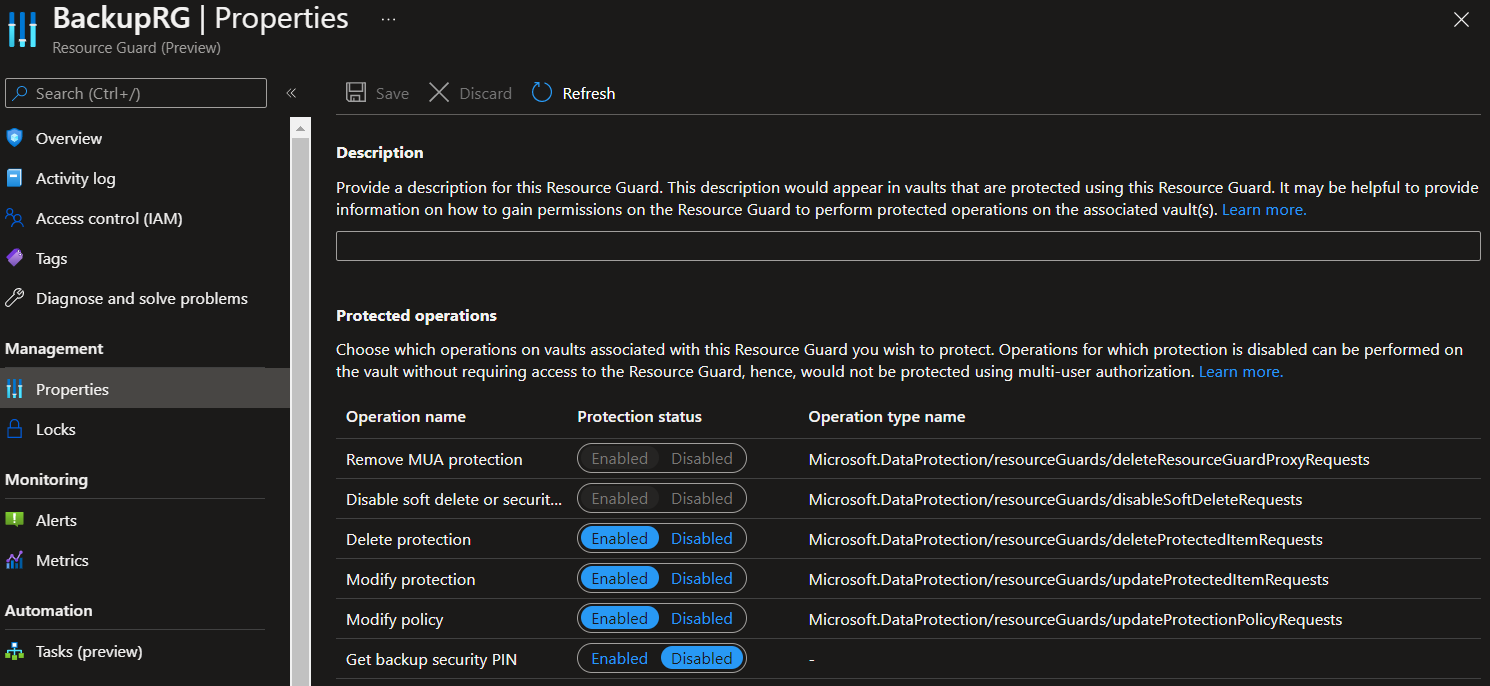
\includegraphics[width=.9\linewidth]{figures/RG-properties.PNG}
%Define properties for width etc.

\subsection{Assigning reader role to backup admin}
The next step is to assign the reader role on the Resource Guard to the backup administrator account. In the GUI we can do this through the Access control(IAM)-blads. In the following images we add the reader role on the Resource guard to the user that acts as the backup admin in this example.

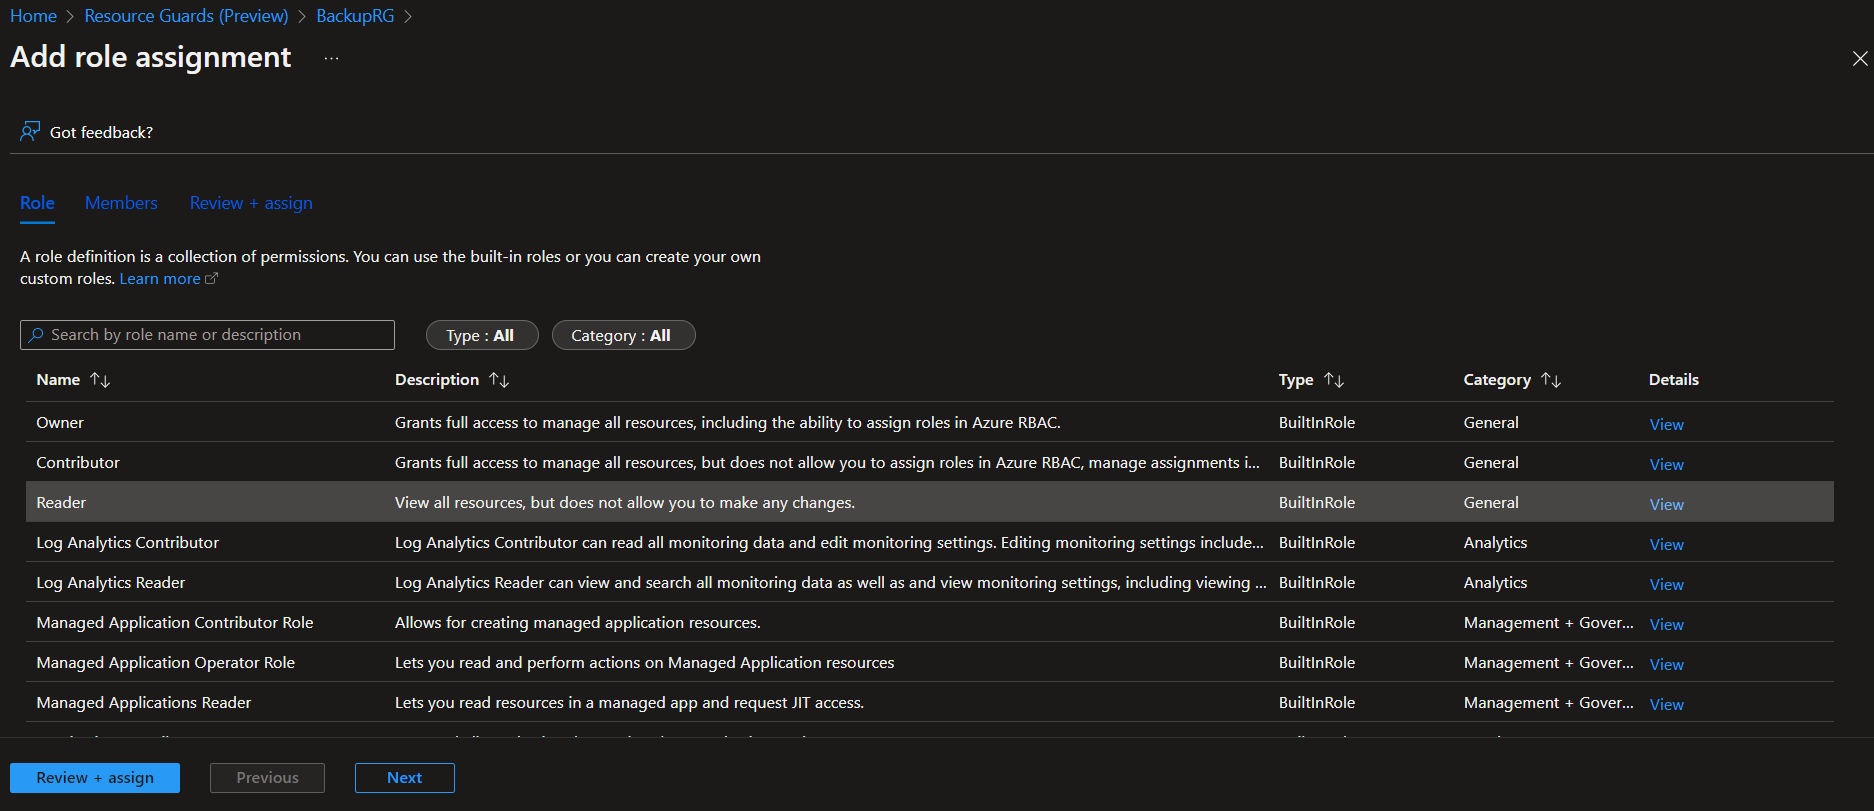
\includegraphics[width=.9\linewidth]{figures/RG-roles.PNG}

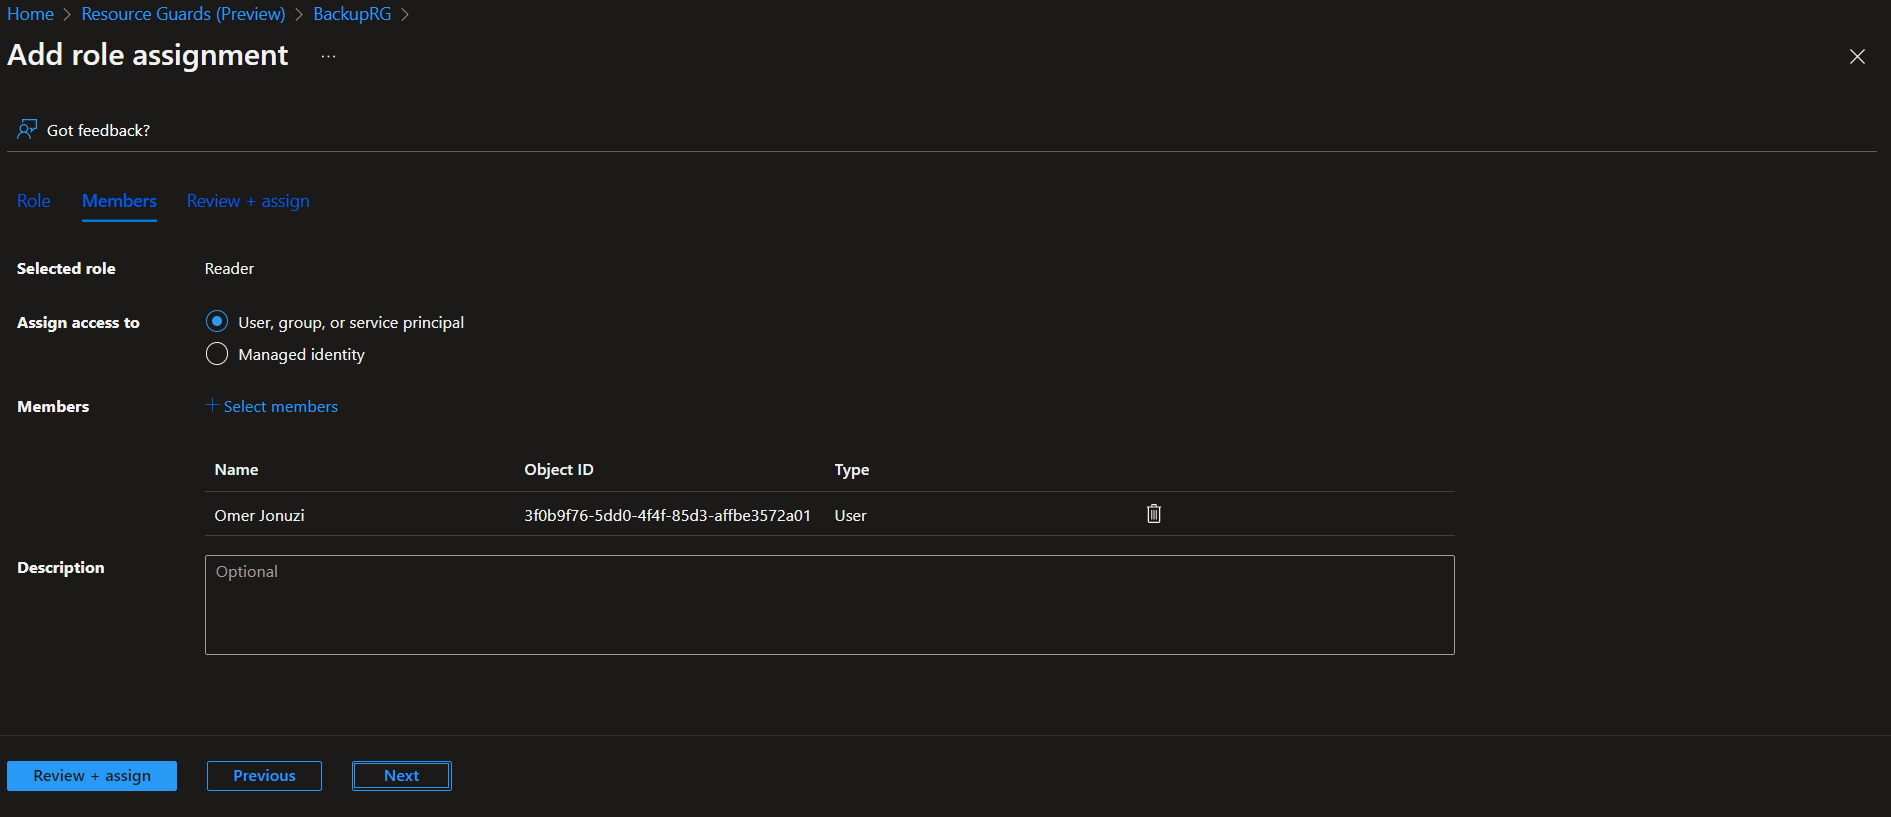
\includegraphics[width=.9\linewidth]{figures/RG-user.PNG}

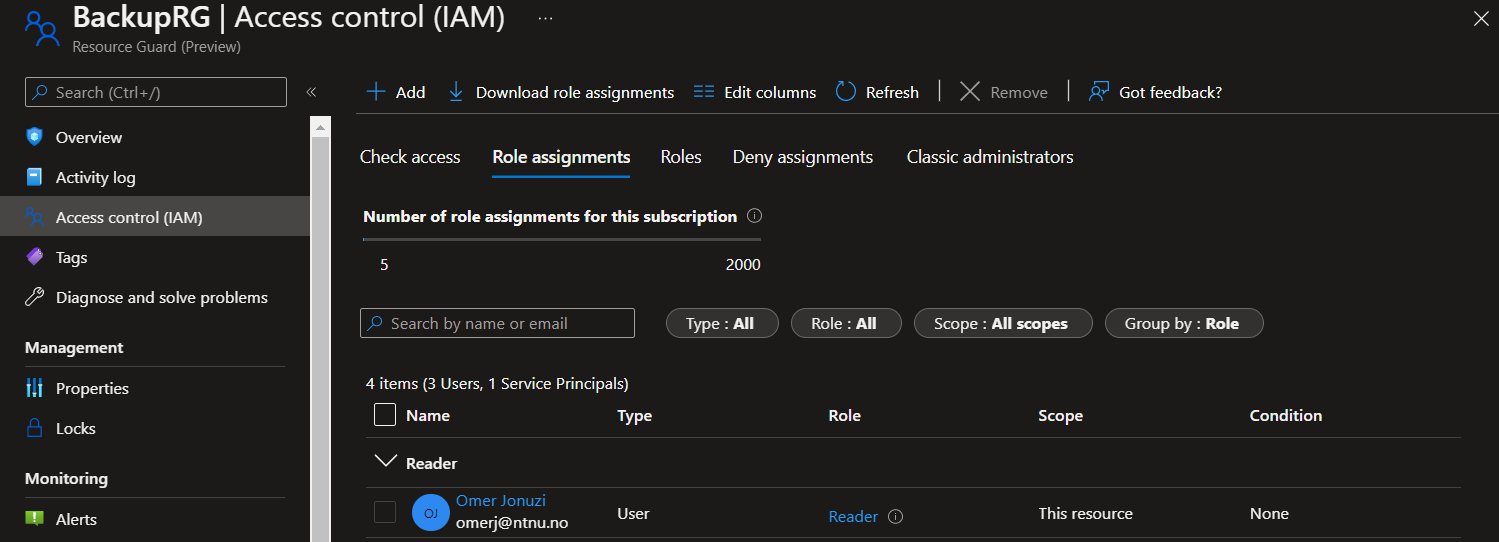
\includegraphics[width=.9\linewidth]{figures/RG-ACblade.PNG}


After the reader role has been granted, the backup administrator can choose to protect any Recovery Service vault with multi-user authorization. To do this they must choose which resource guard to protect it with, which is why the reader role is required. If they do, any protected operation, such as disabling soft-delete or turning MUA off again, should fail as they do not have the necessary permissions on the resource guard. 

\subsection{Applying MUA to vault}
\label{app:chs3e3}
We created a Recovery Services vault, added a resource guard and attempted to disable soft delete.

\paragraph{Create a Recovery Services vault}
\label{sec:org0ba319f}
Since the RSV was deleted in the last experiment,
we made a new one.

Create RSV:
\begin{minted}[breaklines=true,breakanywhere=true]{powershell}
az backup vault create --location $location --name $RSVName --resource-group $RGName
\end{minted}

Output:
\begin{minted}[breaklines=true,breakanywhere=true]{json}
{
  "etag": "W/\"datetime'2022-05-13T13%3A13%3A28.4632743Z'\"",
  "id": "/subscriptions/4b48eb85-91f3-4902-b74b-e84641fb6785/resourceGroups/testRG/providers/Microsoft.RecoveryServices/vaults/myRSV",
  "identity": null,
  "location": "eastus",
  "name": "myRSV",
  "properties": {
    "encryption": null,
    "privateEndpointConnections": null,
    "privateEndpointStateForBackup": "None",
    "privateEndpointStateForSiteRecovery": "None",
    "provisioningState": "Succeeded",
    "upgradeDetails": null
  },
  "resourceGroup": "testRG",
  "sku": {
    "name": "Standard",
    "tier": null
  },
  "systemData": null,
  "tags": null,
  "type": "Microsoft.RecoveryServices/vaults"
}
\end{minted}
\paragraph{Add resource guard}
\label{sec:org4eeccf2}
Press update MUA settings:
\begin{center}
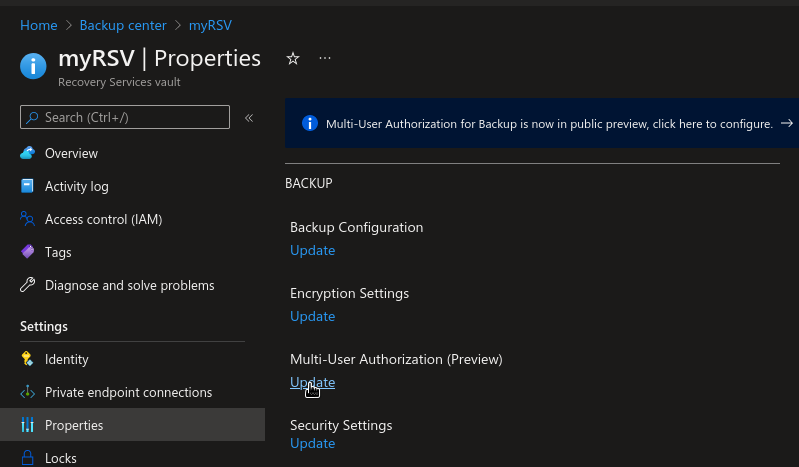
\includegraphics[width=.9\linewidth]{figures/mua/update_rsv_mua.png}
\end{center}

Select resource guard:
\begin{center}
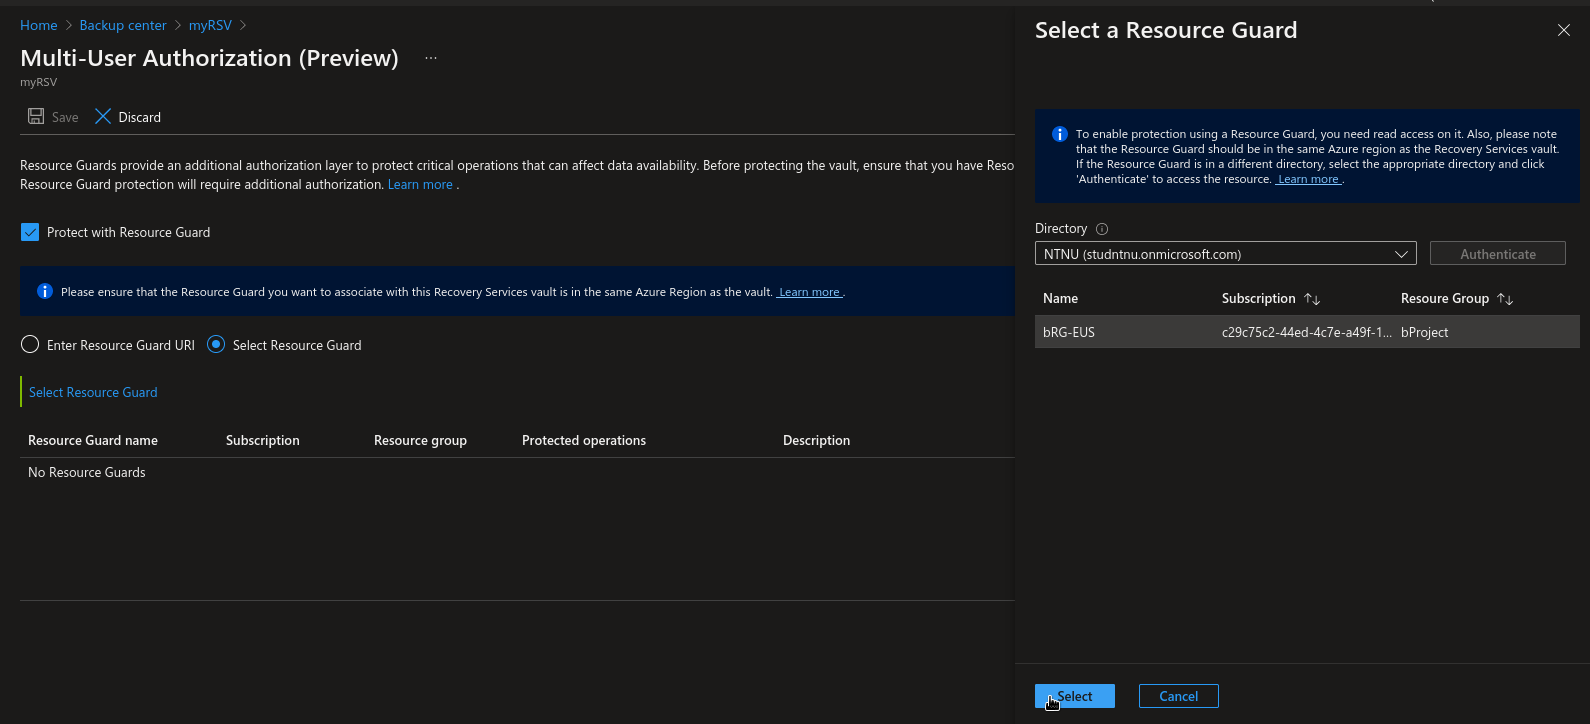
\includegraphics[width=.9\linewidth]{figures/mua/select_resource_guard.png}
\end{center}

Save settings:
\begin{center}
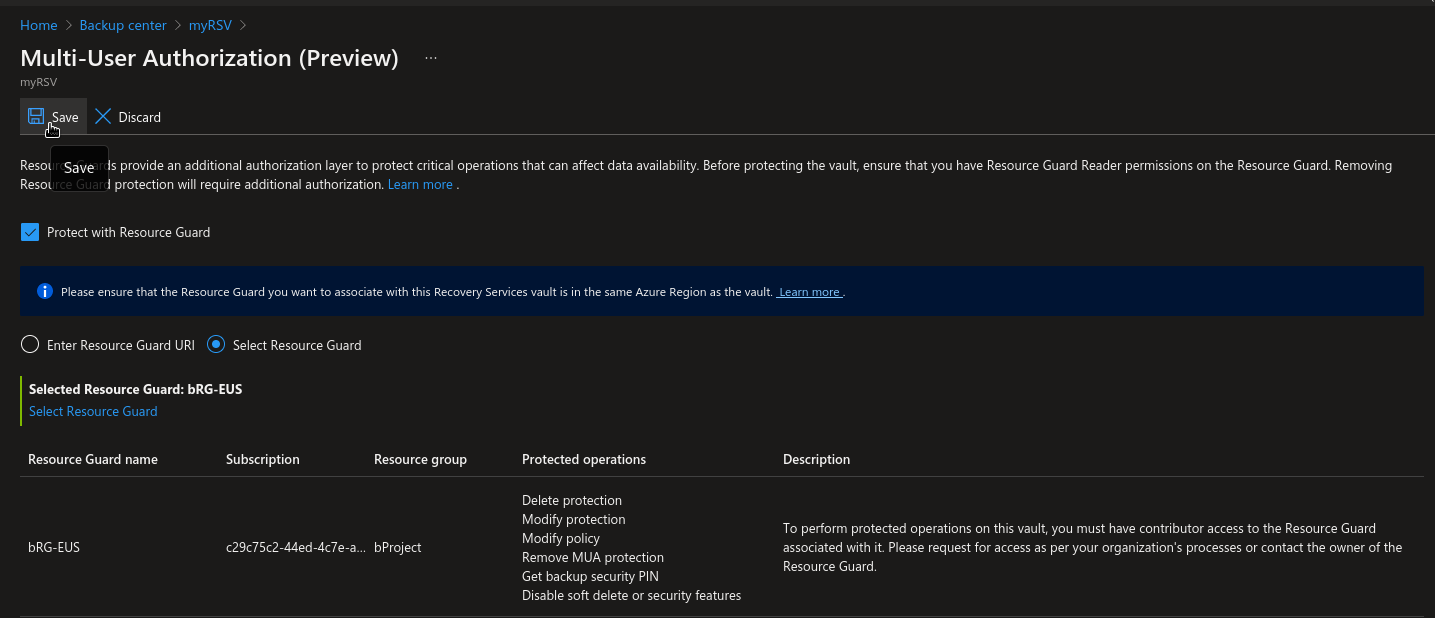
\includegraphics[width=.9\linewidth]{figures/mua/save_mua_settings.png}
\end{center}

\subsection{Testing protected action}
\paragraph{Try to disable soft delete via Azure CLI}
\label{sec:org532e6eb}
An attempt was made at disabling soft delete via the Azure CLI.
The request failed with a generic ``BadRequest'' status code,
presumably because of MUA.

\begin{minted}[breaklines=true,breakanywhere=true]{powershell}
# Get RSV
$RSV = Get-AzRecoveryServicesVault -Name $RSVName -ResourceGroupName $RGName

# Disable soft delete
Set-AzRecoveryServicesVaultProperty -VaultId $RSV.ID -SoftDeleteFeatureState Disable
# Set-AzRecoveryServicesVaultProperty: One or more errors occurred. (Operation returned an invalid status code 'BadRequest')
\end{minted}

\paragraph{Try to disable soft delete via Azure Portal}
\label{sec:orgf58e754}
We attempted to disable soft delete via the Azure Portal.

Disabling soft delete for the vault:
\begin{center}
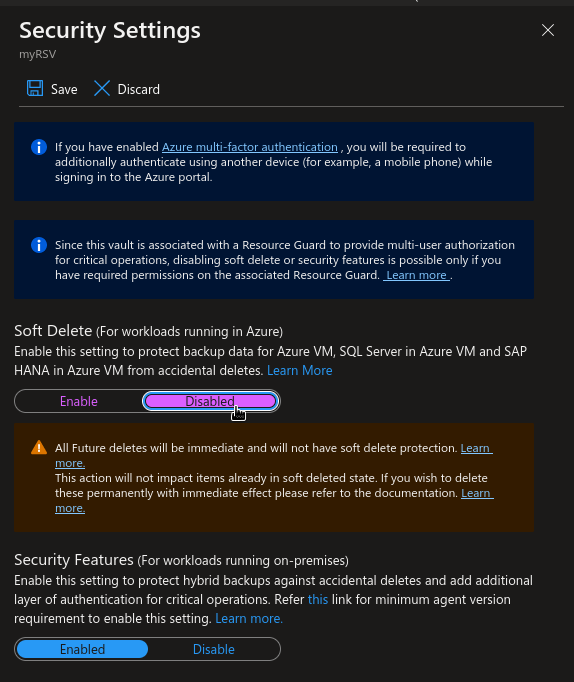
\includegraphics[width=.9\linewidth]{figures/mua/disable_soft_delete.png}
\end{center}

An error appeared in the notifications:
\begin{center}
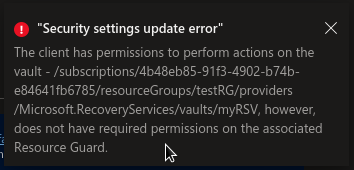
\includegraphics[width=.9\linewidth]{figures/mua/error_mua.png}
\end{center}

\paragraph{Try to run RSV deletion script}
\label{sec:org5bccee7}
The script from [cref] was run once again.
It appears it was able to delete the vault.
We believe this is because the vault is empty.
We attempted a second time with a vault containing backup data.

Output from script:
\begin{minted}[breaklines=true,breakanywhere=true]{text}
Name                                     Account                           SubscriptionName                  Environment                      TenantId
----                                     -------                           ----------------                  -----------                      --------
Azure for Students (4b48eb85-91f3-4902-… MSI@50342                         Azure for Students                AzureCloud                       09a10672-822f-4467-a5ba-5bb3759…

ResourceName      : myRSV
ResourceGroupName : testRG
ResourceNamespace : Microsoft.RecoveryServices
ResouceType       : vaults

Set-AzRecoveryServicesVaultProperty: /home/torstein/delete-rsv.ps1:12
Line |
  12 |  Set-AzRecoveryServicesVaultProperty -Vault $VaultToDelete.ID -SoftDel …
     |  ~~~~~~~~~~~~~~~~~~~~~~~~~~~~~~~~~~~~~~~~~~~~~~~~~~~~~~~~~~~~~~~~~~~~~
     | One or more errors occurred. (Operation returned an invalid status code 'BadRequest')

Soft delete disabled for the vault myRSV
Invoke-RestMethod: /home/torstein/delete-rsv.ps1:30
Line |
  30 |  $response = Invoke-RestMethod -Uri $restUri -Headers $authHeader -Bod …
     |              ~~~~~~~~~~~~~~~~~~~~~~~~~~~~~~~~~~~~~~~~~~~~~~~~~~~~~~~~~
     | {"error":{"code":"InvalidSubscriptionId","message":"The provided subscription identifier 'Azure for Students' is malformed or invalid."}}

Disabled and deleted Azure VM backup items
Disabled and deleted SQL Server backup items
Disabled auto-protection and deleted SQL protectable items
Deleted SQL Servers in Azure VM containers
Disabled and deleted SAP HANA backup items
Deleted SAP HANA in Azure VM containers
Disabled and deleted Azure File Share backups
Unregistered Storage Accounts
Deleted MARS Servers
Deleted MAB Servers
Deleted DPM Servers
Removed Private Endpoints
Number of backup items left in the vault and which need to be deleted: 0 Azure VMs 0 SQL Server Backup Items 0 SQL Server Backup Containers 0 SQL Server Instances 0 SAP HANA backup items 0 SAP HANA Backup Containers 0 Azure File Shares 0 Storage Accounts 0 MARS Servers 0 MAB Servers 0 DPM Servers 0 Private endpoints
Number of ASR items left in the vault and which need to be deleted: 0 ASR protected items 0 ASR policy mappings 0 ASR Fabrics 0 Private endpoints. Warning: This script will only remove the replication configuration from Azure Site Recovery and not from the source. Please cleanup the source manually. Visit https://go.microsoft.com/fwlink/?linkid=2182781 to learn more

Response : Vault has been deleted
\end{minted}

List RSVs:
\begin{minted}[breaklines=true,breakanywhere=true]{powershell}
az backup vault list
\end{minted}

\begin{minted}[breaklines=true,breakanywhere=true]{json}
[
  {
    "etag": "W/\"datetime'2022-05-10T09%3A58%3A14.2637541Z'\"",
    "id": "/subscriptions/4b48eb85-91f3-4902-b74b-e84641fb6785/resourceGroups/perfRG/providers/Microsoft.RecoveryServices/vaults/perfRSV",
    "identity": null,
    "location": "eastus",
    "name": "perfRSV",
    "properties": {
      "encryption": null,
      "privateEndpointConnections": null,
      "privateEndpointStateForBackup": "None",
      "privateEndpointStateForSiteRecovery": "None",
      "provisioningState": "Succeeded",
      "upgradeDetails": null
    },
    "resourceGroup": "perfRG",
    "sku": {
      "name": "Standard",
      "tier": null
    },
    "systemData": null,
    "tags": null,
    "type": "Microsoft.RecoveryServices/vaults"
  }
]
\end{minted}

``myRSV'' is not present in the list.

\paragraph{create new RSV and back up an item}
\label{sec:org3570275}
Create RSV:
\begin{minted}[breaklines=true,breakanywhere=true]{powershell}
az backup vault create --location $location --name $RSVName --resource-group $RGName
\end{minted}

Back up VM:
\begin{minted}[breaklines=true,breakanywhere=true]{powershell}
az backup protection enable-for-vm `
 --resource-group $RGName `
 --vault-name $RSVName `
 --vm $CHName `
 --policy-name $PolicyName
\end{minted}

\paragraph{Add resource guard}
\label{sec:orgc3c211b}
The same procedure was followed as in \hyperref[sec:org4eeccf2]{Add resource guard}.

\paragraph{Try to run RSV deletion script}
\label{sec:orgbb61506}
The script was run once again.
This time, we got a few more errors.
The script still claims that soft delete was disabled,
and that VMs were deleted, but this appears not to be the case.

Output from script:
\begin{minted}[breaklines=true,breakanywhere=true]{text}
Name                                     Account                           SubscriptionName                  Environment                      TenantId
----                                     -------                           ----------------                  -----------                      --------
Azure for Students (4b48eb85-91f3-4902-… MSI@50342                         Azure for Students                AzureCloud                       09a10672-822f-4467-a5ba-5bb3759…

ResourceName      : myRSV
ResourceGroupName : testRG
ResourceNamespace : Microsoft.RecoveryServices
ResouceType       : vaults

Set-AzRecoveryServicesVaultProperty: /home/torstein/delete-rsv.ps1:12
Line |
  12 |  Set-AzRecoveryServicesVaultProperty -Vault $VaultToDelete.ID -SoftDel …
     |  ~~~~~~~~~~~~~~~~~~~~~~~~~~~~~~~~~~~~~~~~~~~~~~~~~~~~~~~~~~~~~~~~~~~~~
     | One or more errors occurred. (Operation returned an invalid status code 'BadRequest')

Soft delete disabled for the vault myRSV
Invoke-RestMethod: /home/torstein/delete-rsv.ps1:30
Line |
  30 |  $response = Invoke-RestMethod -Uri $restUri -Headers $authHeader -Bod …
     |              ~~~~~~~~~~~~~~~~~~~~~~~~~~~~~~~~~~~~~~~~~~~~~~~~~~~~~~~~~
     | {"error":{"code":"InvalidSubscriptionId","message":"The provided subscription identifier 'Azure for Students' is malformed or invalid."}}

Disable-AzRecoveryServicesBackupProtection: /home/torstein/delete-rsv.ps1:49
Line |
  49 |          Disable-AzRecoveryServicesBackupProtection -Item $item -Vault …
     |          ~~~~~~~~~~~~~~~~~~~~~~~~~~~~~~~~~~~~~~~~~~~~~~~~~~~~~~~~~~~~~
     | Unlock privilege access is needed to delete the ResourceGuard proxy

Disabled and deleted Azure VM backup items
Disabled and deleted SQL Server backup items
Disabled auto-protection and deleted SQL protectable items
Deleted SQL Servers in Azure VM containers
Disabled and deleted SAP HANA backup items
Deleted SAP HANA in Azure VM containers
Disabled and deleted Azure File Share backups
Unregistered Storage Accounts
Deleted MARS Servers
Deleted MAB Servers
Deleted DPM Servers
Removed Private Endpoints
Number of backup items left in the vault and which need to be deleted: 1 Azure VMs 0 SQL Server Backup Items 0 SQL Server Backup Containers 0 SQL Server Instances 0 SAP HANA backup items 0 SAP HANA Backup Containers 0 Azure File Shares 0 Storage Accounts 0 MARS Servers 0 MAB Servers 0 DPM Servers 0 Private endpoints
Number of ASR items left in the vault and which need to be deleted: 0 ASR protected items 0 ASR policy mappings 0 ASR Fabrics 0 Private endpoints. Warning: This script will only remove the replication configuration from Azure Site Recovery and not from the source. Please cleanup the source manually. Visit https://go.microsoft.com/fwlink/?linkid=2182781 to learn more
Remove-AzRecoveryServicesVault: /home/torstein/delete-rsv.ps1:204
Line |
 204 |  Remove-AzRecoveryServicesVault -Vault $VaultToDelete
     |  ~~~~~~~~~~~~~~~~~~~~~~~~~~~~~~~~~~~~~~~~~~~~~~~~~~~~
     | Operation failed. ClientRequestId: 9e041d38-0531-4dbb-8db8-63ec5f59f341-2022-05-13 13:41:03Z-P One or more errors occurred. (Recovery Services Vault cannot
     | be deleted as there are existing resources within the vault.  : clickhouseVM. Please ensure all containers have been unregistered from the vault and all
     | private endpoints associated with the vault have been deleted, and retry operation. For more details, see https://aka.ms/AB-AA4ecq5)
\end{minted}

List RSVs:
\begin{minted}[breaklines=true,breakanywhere=true]{powershell}
az backup vault list
\end{minted}

Output:
\begin{minted}[breaklines=true,breakanywhere=true]{json}
[
  {
    "etag": "W/\"datetime'2022-05-10T09%3A58%3A14.2637541Z'\"",
    "id": "/subscriptions/4b48eb85-91f3-4902-b74b-e84641fb6785/resourceGroups/perfRG/providers/Microsoft.RecoveryServices/vaults/perfRSV",
    "identity": null,
    "location": "eastus",
    "name": "perfRSV",
    "properties": {
      "encryption": null,
      "privateEndpointConnections": null,
      "privateEndpointStateForBackup": "None",
      "privateEndpointStateForSiteRecovery": "None",
      "provisioningState": "Succeeded",
      "upgradeDetails": null
    },
    "resourceGroup": "perfRG",
    "sku": {
      "name": "Standard",
      "tier": null
    },
    "systemData": null,
    "tags": null,
    "type": "Microsoft.RecoveryServices/vaults"
  },
  {
    "etag": "W/\"datetime'2022-05-13T13%3A39%3A48.7614362Z'\"",
    "id": "/subscriptions/4b48eb85-91f3-4902-b74b-e84641fb6785/resourceGroups/testRG/providers/Microsoft.RecoveryServices/vaults/myRSV",
    "identity": null,
    "location": "eastus",
    "name": "myRSV",
    "properties": {
      "encryption": null,
      "privateEndpointConnections": null,
      "privateEndpointStateForBackup": "None",
      "privateEndpointStateForSiteRecovery": "None",
      "provisioningState": "Succeeded",
      "upgradeDetails": null
    },
    "resourceGroup": "testRG",
    "sku": {
      "name": "Standard",
      "tier": null
    },
    "systemData": null,
    "tags": null,
    "type": "Microsoft.RecoveryServices/vaults"
  }
]
\end{minted}

The vault (``myRSV'') is still present. In other words the backup administrator was not permitted to delete the vault as long as that involved performing protected actions.

\subsection{Permitting protected actions}
In order to allow for protected actions to be performed on select occasions the reader role will not be sufficient. In order for a backup admin to perform protected actions within a resource guard's scope, they need the contributor-role on that resource guard. In order to to harness the security benefits of just-in-time access and multi user authorization, this can be configured with Azure Active Directory (Azure AD) Privileged Identity Management (PIM). 

The end goal is for the backup admin to be able to raise a request for the contributor role on the resource guard, and temporarily be permitted to perform protected actions. 

In PIM, the security admin must create an eligible assignment for the backup admin as contributor. In short, allowing for the backup admin to request the necessary access. 

In Azure AD privileged identity management we navigate to the resource guard as shown, navigate within it, and click on assignments:

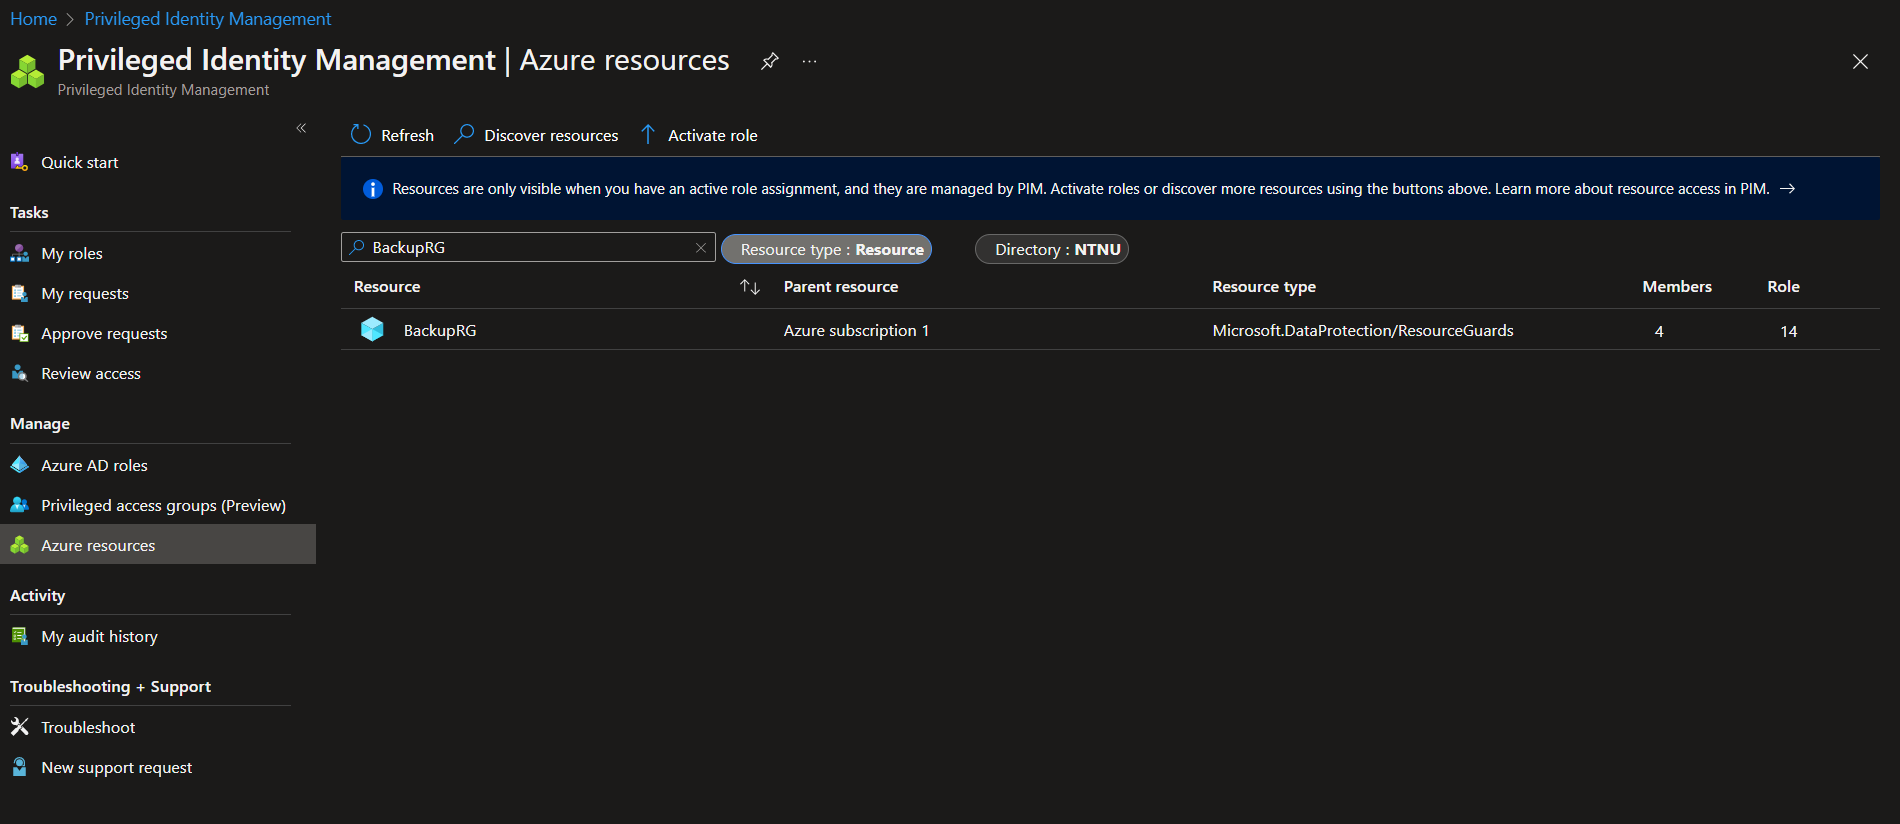
\includegraphics[width=.9\linewidth]{figures/RG-PIM.PNG}

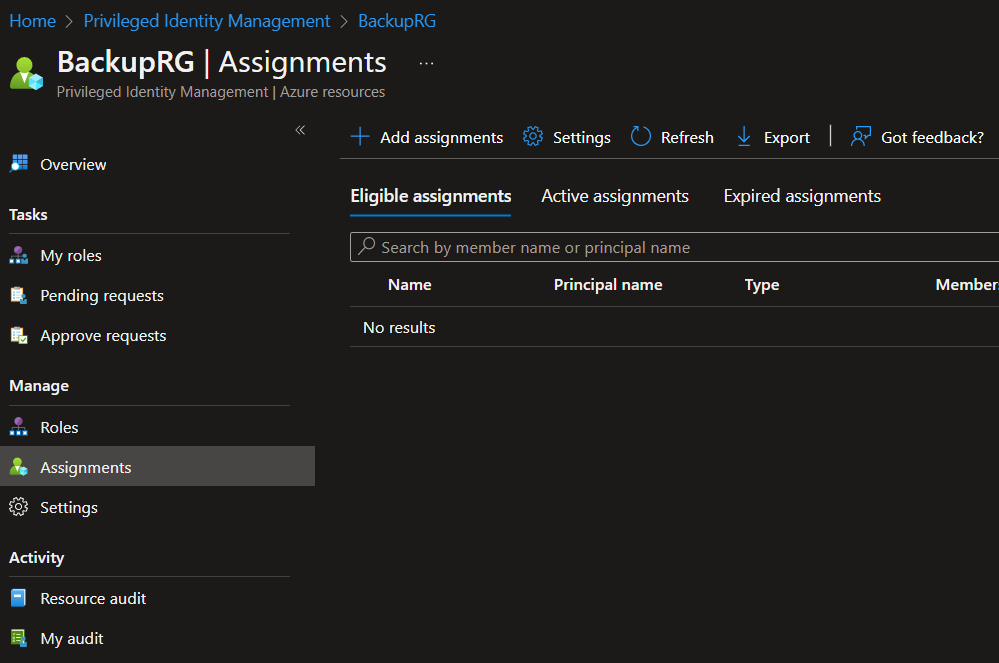
\includegraphics[width=.9\linewidth]{figures/RG-assignments.PNG}

From here we add a new assignment, select the contributor role and our backup admin. THe security admin can choose to grant the assignent for a limitied amount of time, and from here set some settings for maximum duration, and the requirement of a justification before granting the assigned role. By selecting the assignemnt as "elligable", instead of "active", the backup admin must request to have the assigned role activated for them each time they need it. This must then be approved for the amount of time needed until it is automatically revoked. 

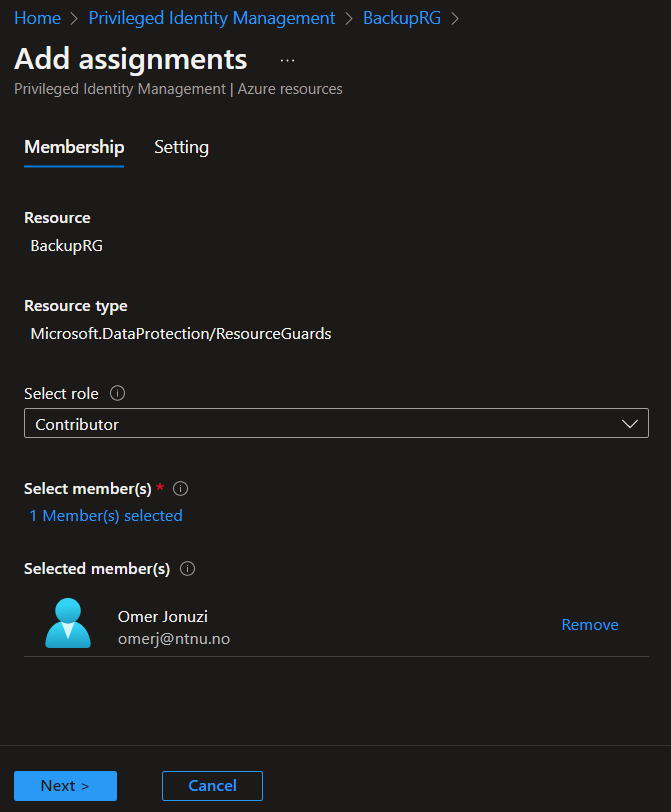
\includegraphics[width=.9\linewidth]{figures/RG-AddAssignment.PNG}

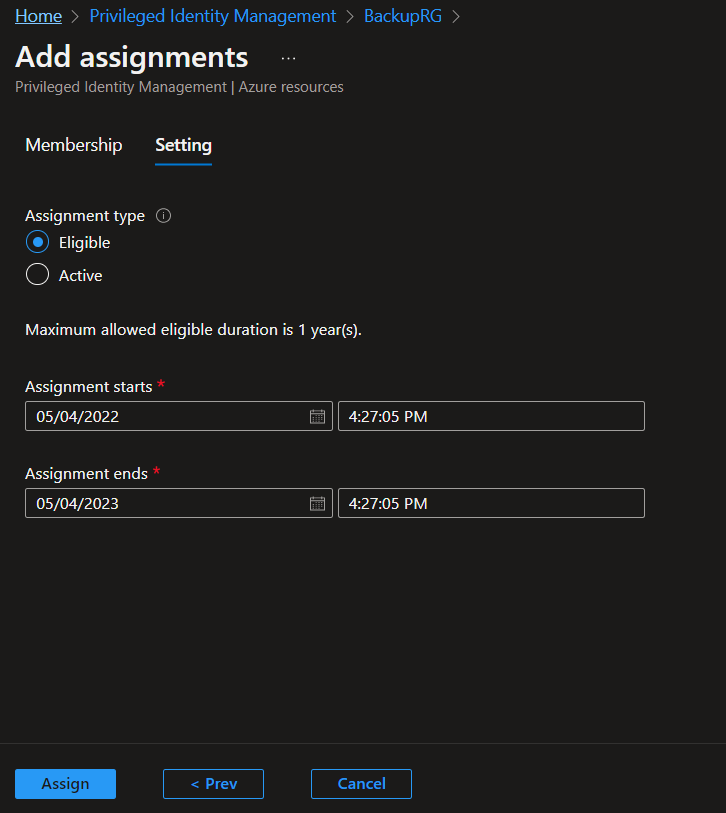
\includegraphics[width=.9\linewidth]{figures/RG-eligible.png}

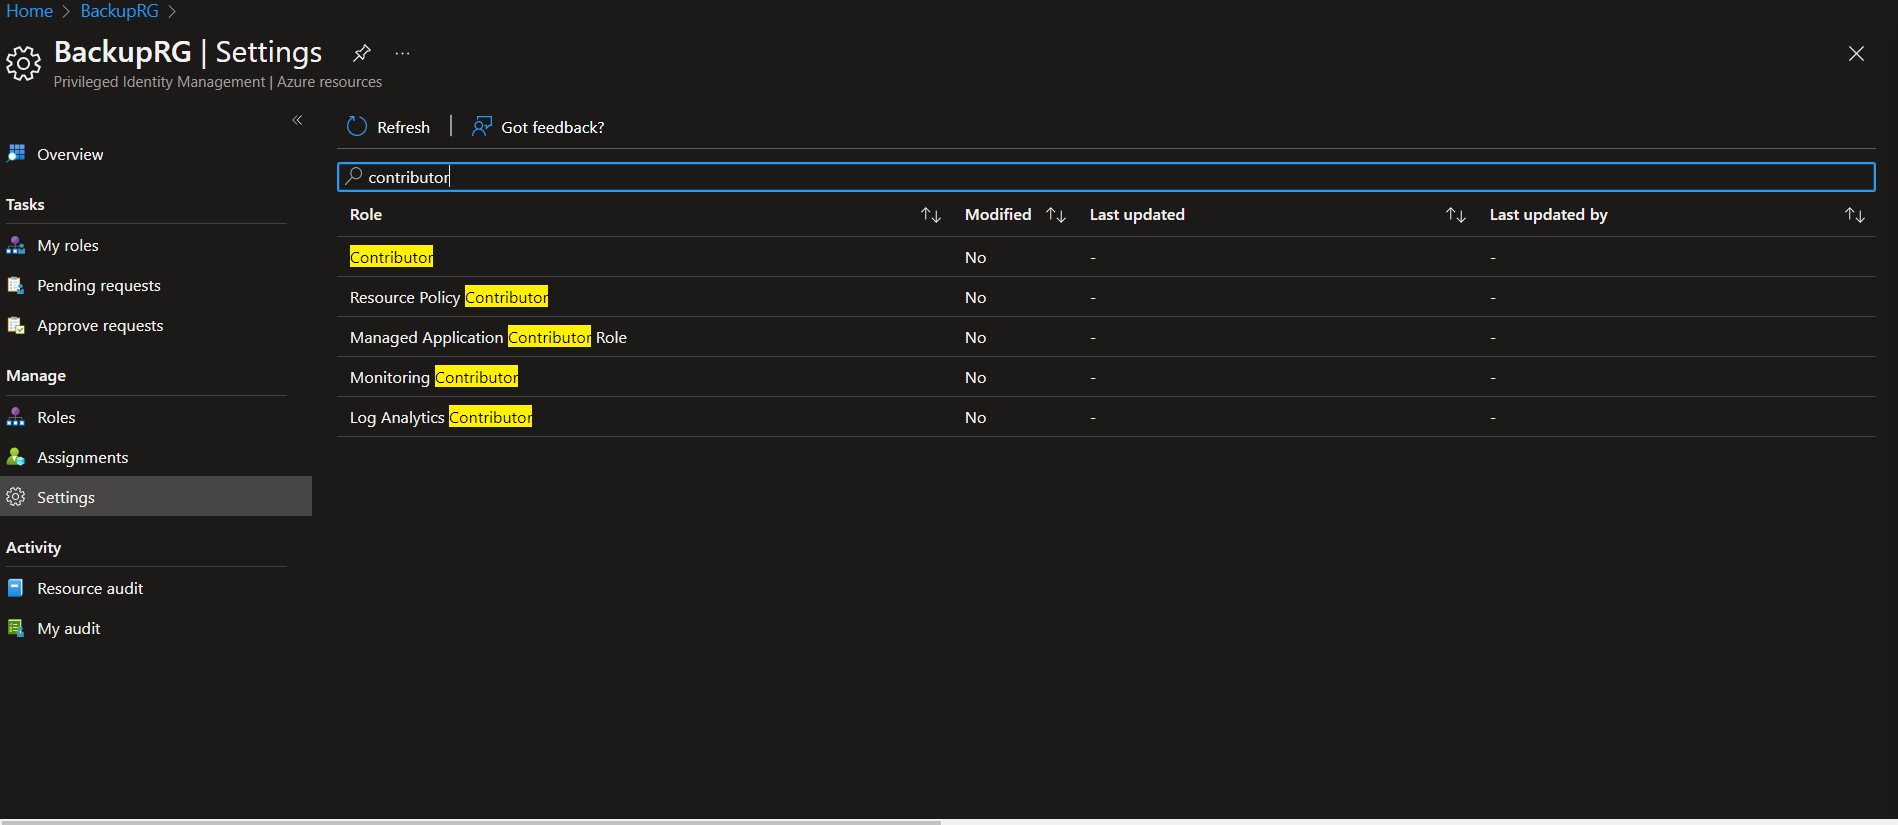
\includegraphics[width=.9\linewidth]{figures/RG-setting.PNG}

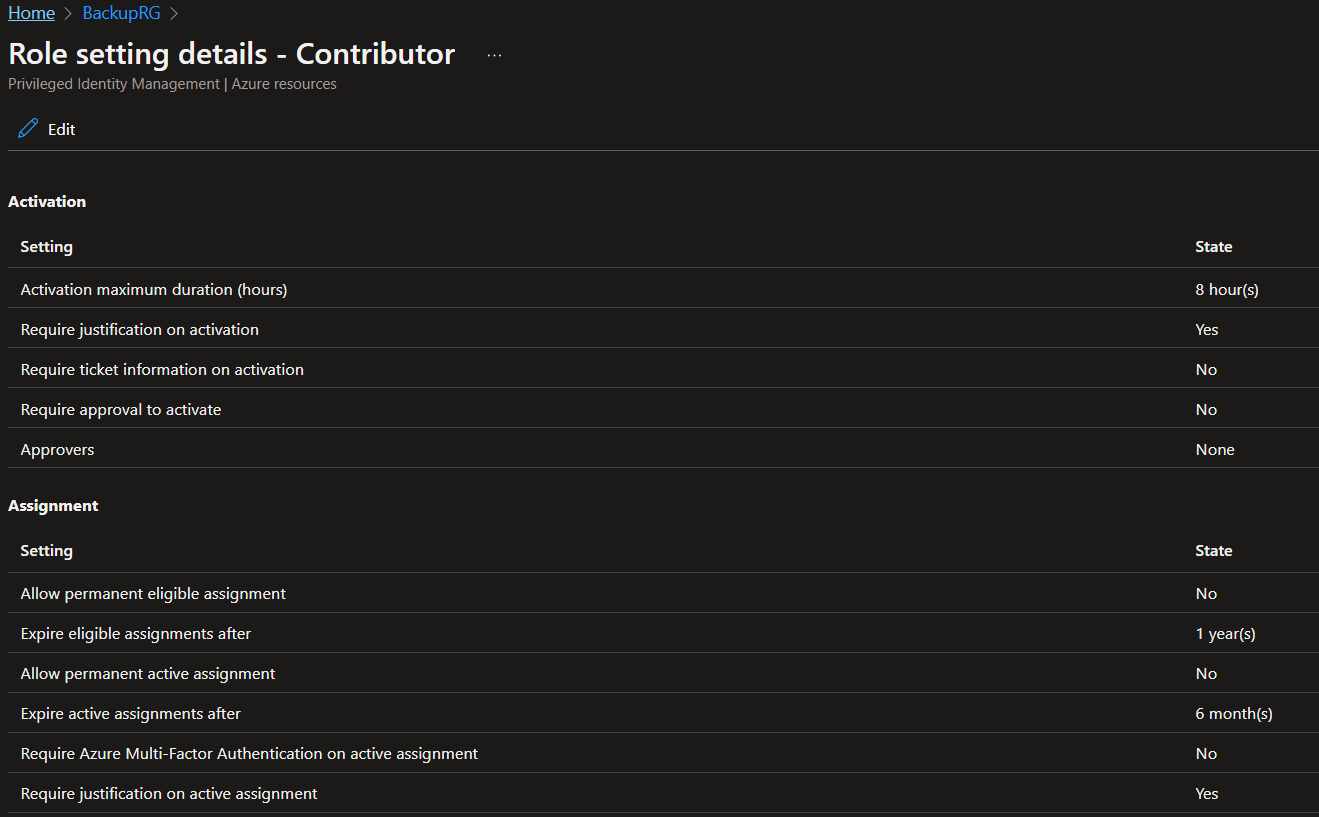
\includegraphics[width=.9\linewidth]{figures/RG-setting-detailts.PNG}

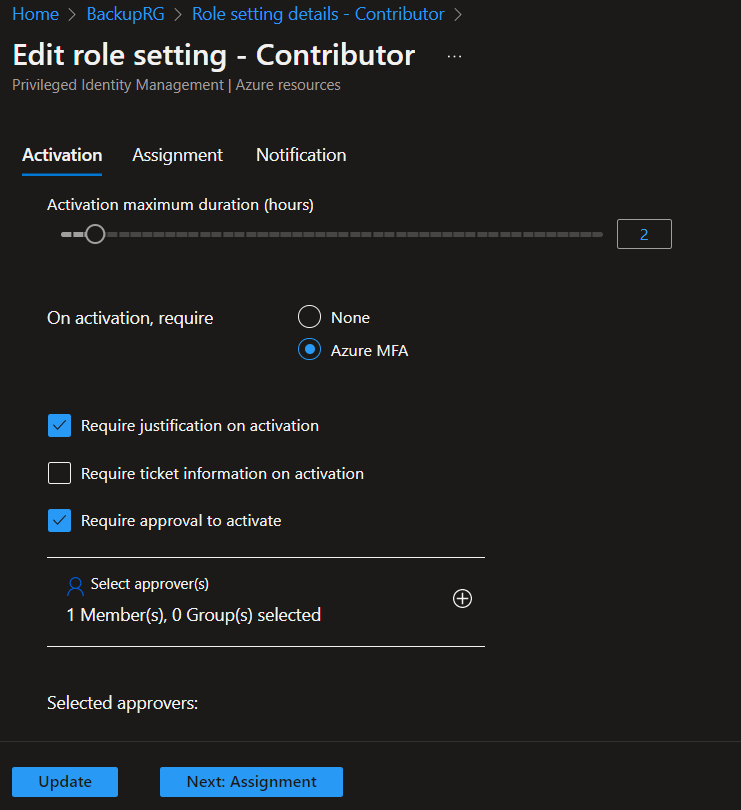
\includegraphics[width=.9\linewidth]{figures/RG-role-setting.PNG}



\paragraph{Request access to contributor role}
\label{sec:orgec87294}
Requesting access to the contributor role:
\begin{center}
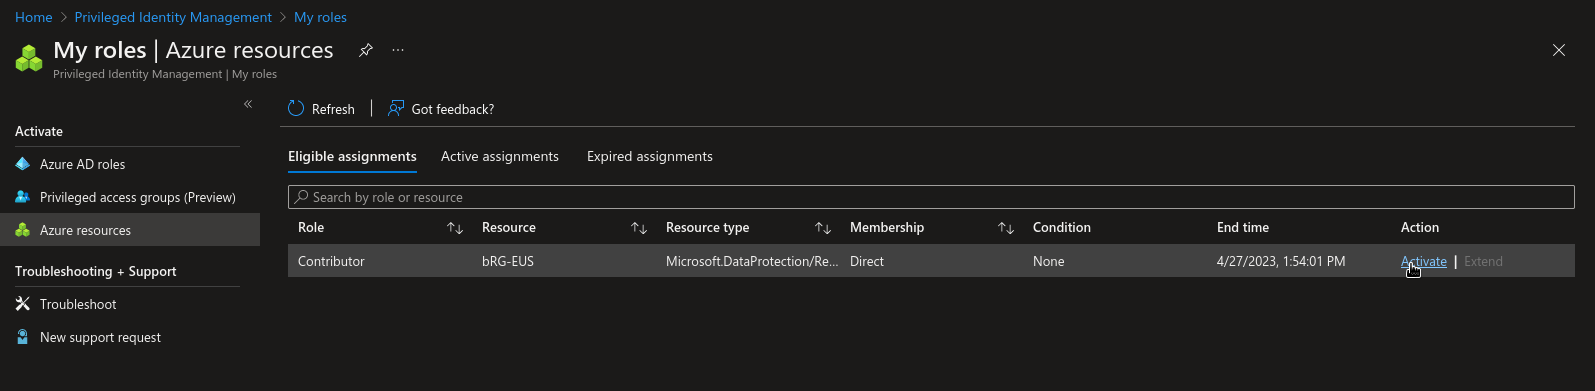
\includegraphics[width=.9\linewidth]{figures/mua/request_role.png}
\end{center}

Sending request:
\begin{center}
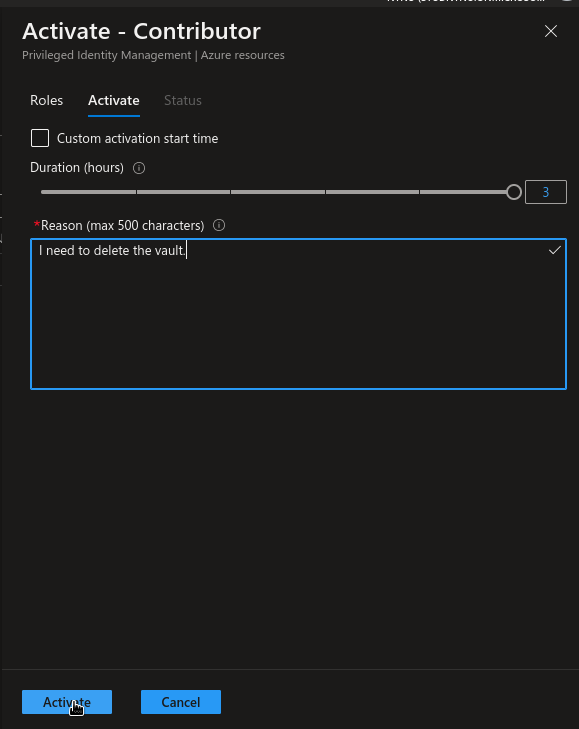
\includegraphics[width=.9\linewidth]{figures/mua/request_mua_role.png}
\end{center}

From the security administrators POV,
A request has been recieived in the PIM-service:

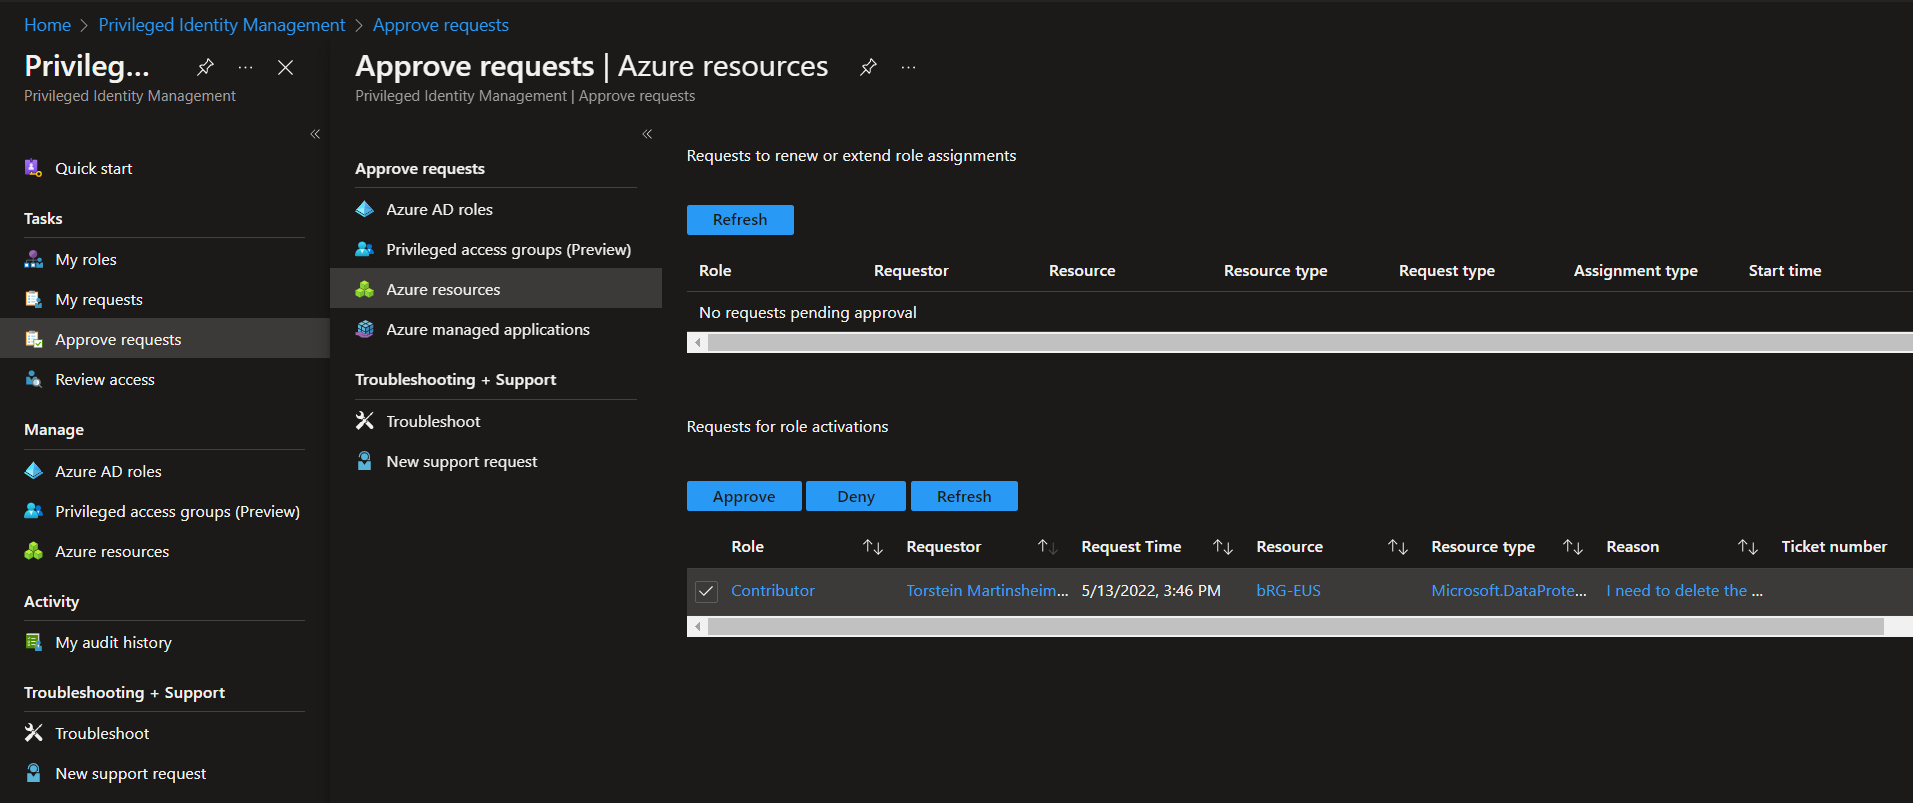
\includegraphics[width=.9\linewidth]{figures/mua/Request.PNG}

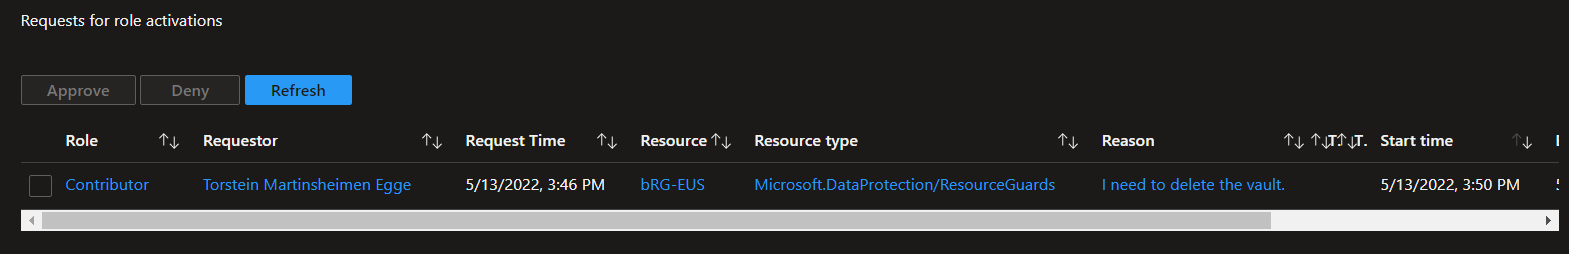
\includegraphics[width=.9\linewidth]{figures/mua/Capture.PNG}

The request is activated by security admin as shown:

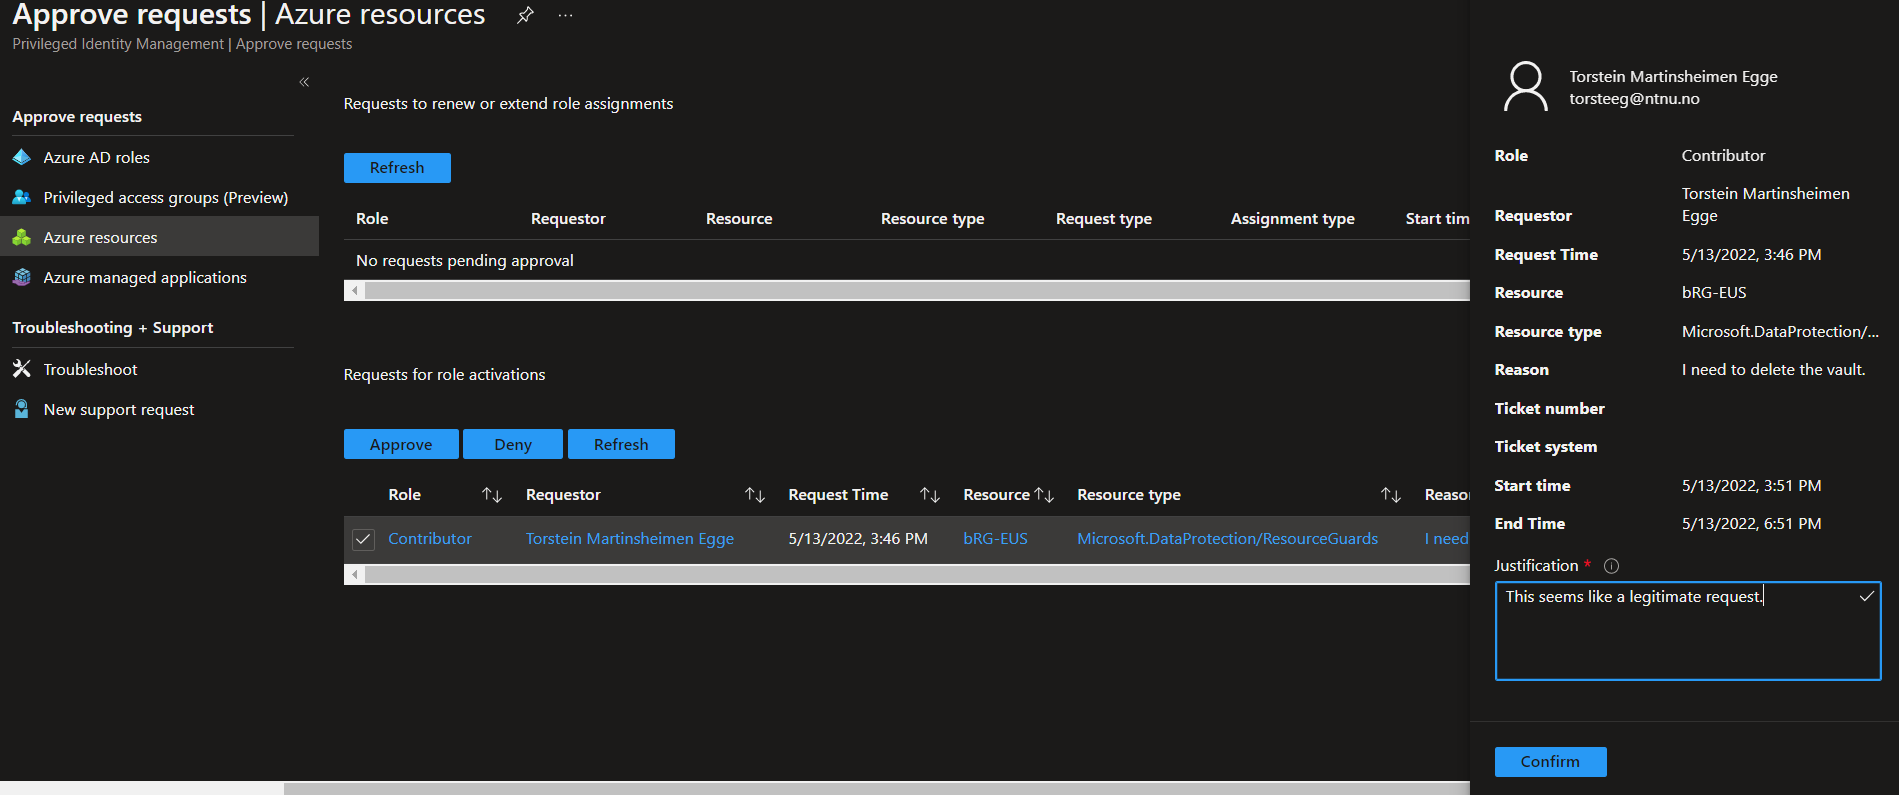
\includegraphics[width=.9\linewidth]{figures/mua/approve.PNG}


An email was received by the backup admin when the request was accepted:
\begin{center}
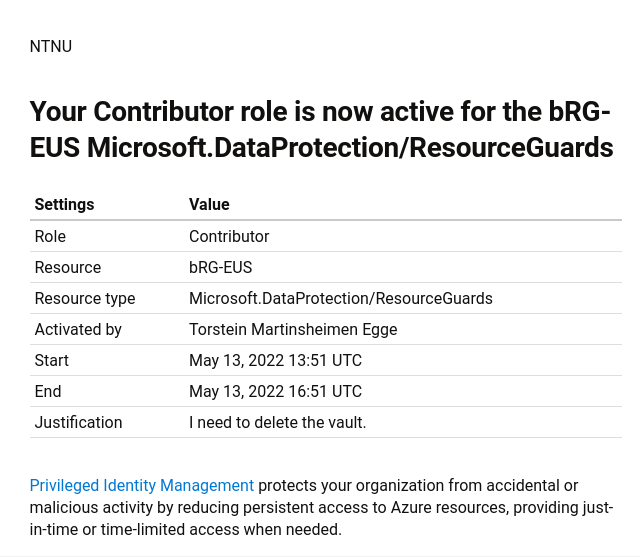
\includegraphics[width=.9\linewidth]{figures/mua/role_active_email.png}
\end{center}

\paragraph{Try to disable soft delete}
\label{sec:org6ff9cf1}
Soft delete was successfully disabled for the vault:
\begin{center}
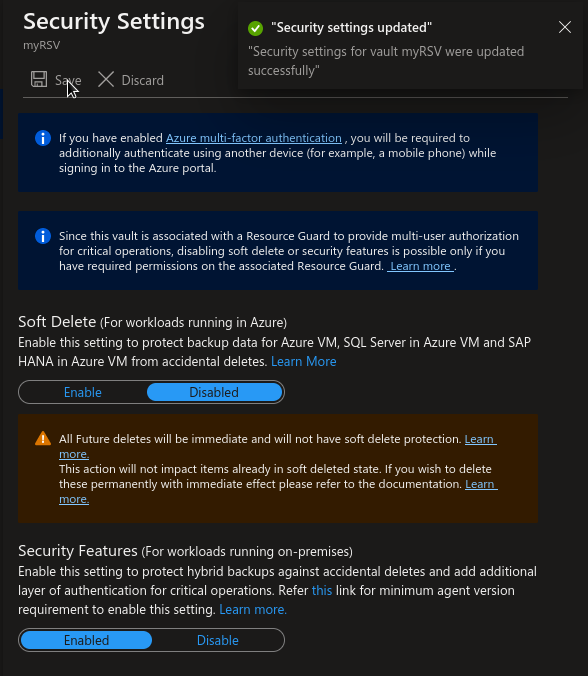
\includegraphics[width=.9\linewidth]{figures/mua/soft_delete_disabled.png}
\end{center}

 \section{Restore from a backup vault}
\label{app:pg-restore1}
\begin{minted}[breaklines=true,breakanywhere=true]{json}
{
   "authorization": {
       "action": "Microsoft.DataProtection/backupVaults/backupInstances/restore/action",
       "scope": "/subscriptions/3d440288-2774-4e29-b3d7-0b9efe86bba7/resourceGroups/bachelor119/providers/Microsoft.DataProtection/backupVaults/bachelor119-performance-backup/backupInstances/bachelor119-performance-postgres-748e4aca-e53b-4e15-9fe2-665e67d8c03e"
   },
   "caller": "omerj@ntnu.no",
   "channels": "Operation",
   "claims": {
       "aud": "https://management.core.windows.net/",
       "iss": "https://sts.windows.net/09a10672-822f-4467-a5ba-5bb375967c05/",
       "iat": "1651736576",
       "nbf": "1651736576",
       "exp": "1651741076",
       "http://schemas.microsoft.com/claims/authnclassreference": "1",
       "aio": "AVQAq/8TAAAABL3Z7ULGAW1yexY77bzlzAyhUVgZSwf0iL4jELLfgqEExxjWaqv/V018J4GhfqQcZV9PkxbGEDAvPyhTqxWWhMQVZu9S5OlQB4Ev2uHhnTE=",
       "http://schemas.microsoft.com/claims/authnmethodsreferences": "pwd,mfa",
       "appid": "c44b4083-3bb0-49c1-b47d-974e53cbdf3c",
       "appidacr": "2",
       "http://schemas.xmlsoap.org/ws/2005/05/identity/claims/surname": "Jonuzi",
       "http://schemas.xmlsoap.org/ws/2005/05/identity/claims/givenname": "Omer",
       "groups": "8d15c301-2022-4dc2-9550-f36dbdffee7c,61846c99-b2ae-4898-a10c-2ddd7b4a013f,091bd972-9447-4208-b3cc-8a1959add436,0107c21a-8a63-4b21-87a0-86a12547fd12,94fefe97-5b83-47a6-a829-01b4add29fe3,5f73363b-e2f9-4001-a71d-b6230f44a293,3ef57554-d71c-41a1-a080-701c2320082c,e1adf917-cdb3-42cc-8425-79ffe844a86d,498ce0ed-e83d-413e-b529-bde0346ccdf1,a7f6818e-774d-4e09-994f-77fbe6ff7925,aad00940-a490-41c1-8a0c-9b0be5e7a390,be17024f-57a2-4729-a575-75d7d7b63e14,c497c5c3-4e26-4e2a-8a12-10e0d43288a1,0e414658-efef-4804-a1c4-8a7f668a9e43,7f27023d-8163-41e9-9d11-1cab1ade4d6e,12e6cbdf-815f-478f-8f9d-3c87b6adc5a9,ab6b0bdb-d48d-4c80-bc61-7fca517eb7cf,37309702-9021-40ba-a2d8-3446dca747f2,e1b09d79-d205-4bbe-9d5f-d79df23d5b56,027504c5-23ce-42ae-8aaa-1c4c2df10ead,43a6e580-ca1f-4f8b-b63a-9b1a3e49b72b,46bc9091-e862-4633-bc54-cbf1473fffe9,01fad63f-0f80-4da7-b92a-9bf43062d9c3,2433ef53-9c20-4a85-9c8d-136a4375435d,3a806c10-8ef6-4f00-a9ba-b78faee326a4,587174cf-9b08-44e9-8af5-4d7ac74fa880,9e090282-49ce-4467-94f9-5a85e99c92cf,37dbb3c1-c5f7-4c80-a14a-d622c3775824,0ef51352-b5eb-4cac-a483-a9fa6e536129,8370354f-3451-40b2-9abf-a43e7e62d23d,8103e72f-5acd-4ce9-8c5e-a3af7ba98b36,e29fd27b-746d-4aab-b817-cbc96fc07606,b9e3e345-c7a4-4b86-a1fc-e5b77a8ee6a1,a4295b3f-f9c4-4253-a57a-f42e6ff1a163,9b319622-144f-4573-8a12-a74b6404ca15,b3df6df0-e4ac-44ca-b0c4-27219aaf7e33,6bac6c57-8c80-4639-9691-0ce756fda9ea,a9bafff9-b09e-4124-9d74-482f4d653c4b,5fa55196-5b42-4d47-8599-a724a00435ab,fd780d1e-8cb6-40b2-80cf-acb411f89833,b47da984-e1de-43cc-9149-8fcca0b24340,42d87878-08fe-42f4-9eaa-cd82f1ffc733",
       "ipaddr": "129.241.230.99",
       "name": "Omer Jonuzi",
       "http://schemas.microsoft.com/identity/claims/objectidentifier": "3f0b9f76-5dd0-4f4f-85d3-affbe3572a01",
       "onprem_sid": "S-1-5-21-3959417778-1711865379-3952174976-358665",
       "puid": "100320005758FB15",
       "rh": "0.AQkAcgahCS-CZ0SluluzdZZ8BUZIf3kAutdPukPawfj2MBMJAAM.",
       "http://schemas.microsoft.com/identity/claims/scope": "user_impersonation",
       "http://schemas.xmlsoap.org/ws/2005/05/identity/claims/nameidentifier": "i8uDlYJMGSSdVydTjF8rE7LP1tEpil787X1xYh8H-5I",
       "http://schemas.microsoft.com/identity/claims/tenantid": "09a10672-822f-4467-a5ba-5bb375967c05",
       "http://schemas.xmlsoap.org/ws/2005/05/identity/claims/name": "omerj@ntnu.no",
       "http://schemas.xmlsoap.org/ws/2005/05/identity/claims/upn": "omerj@ntnu.no",
       "uti": "PTjw6g14Z06dvf2WnkwtAA",
       "ver": "1.0",
       "xms_tcdt": "1363351898"
   },
   "correlationId": "0c1c8dd6-246f-412d-9b2a-90baab4b1a1c",
   "description": "",
   "eventDataId": "f714efa3-701c-4673-bcb2-17bcca133cea",
   "eventName": {
       "value": "EndRequest",
       "localizedValue": "End request"
   },
   "category": {
       "value": "Administrative",
       "localizedValue": "Administrative"
   },
   "eventTimestamp": "2022-05-05T08:07:26.1105832Z",
   "id": "/subscriptions/3d440288-2774-4e29-b3d7-0b9efe86bba7/resourceGroups/bachelor119/providers/Microsoft.DataProtection/backupVaults/bachelor119-performance-backup/backupInstances/bachelor119-performance-postgres-748e4aca-e53b-4e15-9fe2-665e67d8c03e/events/f714efa3-701c-4673-bcb2-17bcca133cea/ticks/637873348461105832",
   "level": "Informational",
   "operationId": "c52e2132-8420-446d-b0b8-d7cd42eb2d2e",
   "operationName": {
       "value": "Microsoft.DataProtection/backupVaults/backupInstances/restore/action",
       "localizedValue": "Restore Backup Instance"
   },
   "resourceGroupName": "bachelor119",
   "resourceProviderName": {
       "value": "Microsoft.DataProtection",
       "localizedValue": "Microsoft.DataProtection"
   },
   "resourceType": {
       "value": "Microsoft.DataProtection/backupVaults/backupInstances",
       "localizedValue": "Microsoft.DataProtection/backupVaults/backupInstances"
   },
   "resourceId": "/subscriptions/3d440288-2774-4e29-b3d7-0b9efe86bba7/resourceGroups/bachelor119/providers/Microsoft.DataProtection/backupVaults/bachelor119-performance-backup/backupInstances/bachelor119-performance-postgres-748e4aca-e53b-4e15-9fe2-665e67d8c03e",
   "status": {
       "value": "Succeeded",
       "localizedValue": "Succeeded"
   },
   "subStatus": {
       "value": "",
       "localizedValue": ""
   },
   "submissionTimestamp": "2022-05-05T08:09:10.1063319Z",
   "subscriptionId": "3d440288-2774-4e29-b3d7-0b9efe86bba7",
   "tenantId": "09a10672-822f-4467-a5ba-5bb375967c05",
   "properties": {
       "eventCategory": "Administrative",
       "entity": "/subscriptions/3d440288-2774-4e29-b3d7-0b9efe86bba7/resourceGroups/bachelor119/providers/Microsoft.DataProtection/backupVaults/bachelor119-performance-backup/backupInstances/bachelor119-performance-postgres-748e4aca-e53b-4e15-9fe2-665e67d8c03e",
       "message": "Microsoft.DataProtection/backupVaults/backupInstances/restore/action",
       "hierarchy": "09a10672-822f-4467-a5ba-5bb375967c05/3d440288-2774-4e29-b3d7-0b9efe86bba7"
   },
   "relatedEvents": []
}
\end{minted}
 \section{Postgres: PITR with REST API performance test}
\label{app:pg-restore2}

\begin{figure}[H]
    \centering
    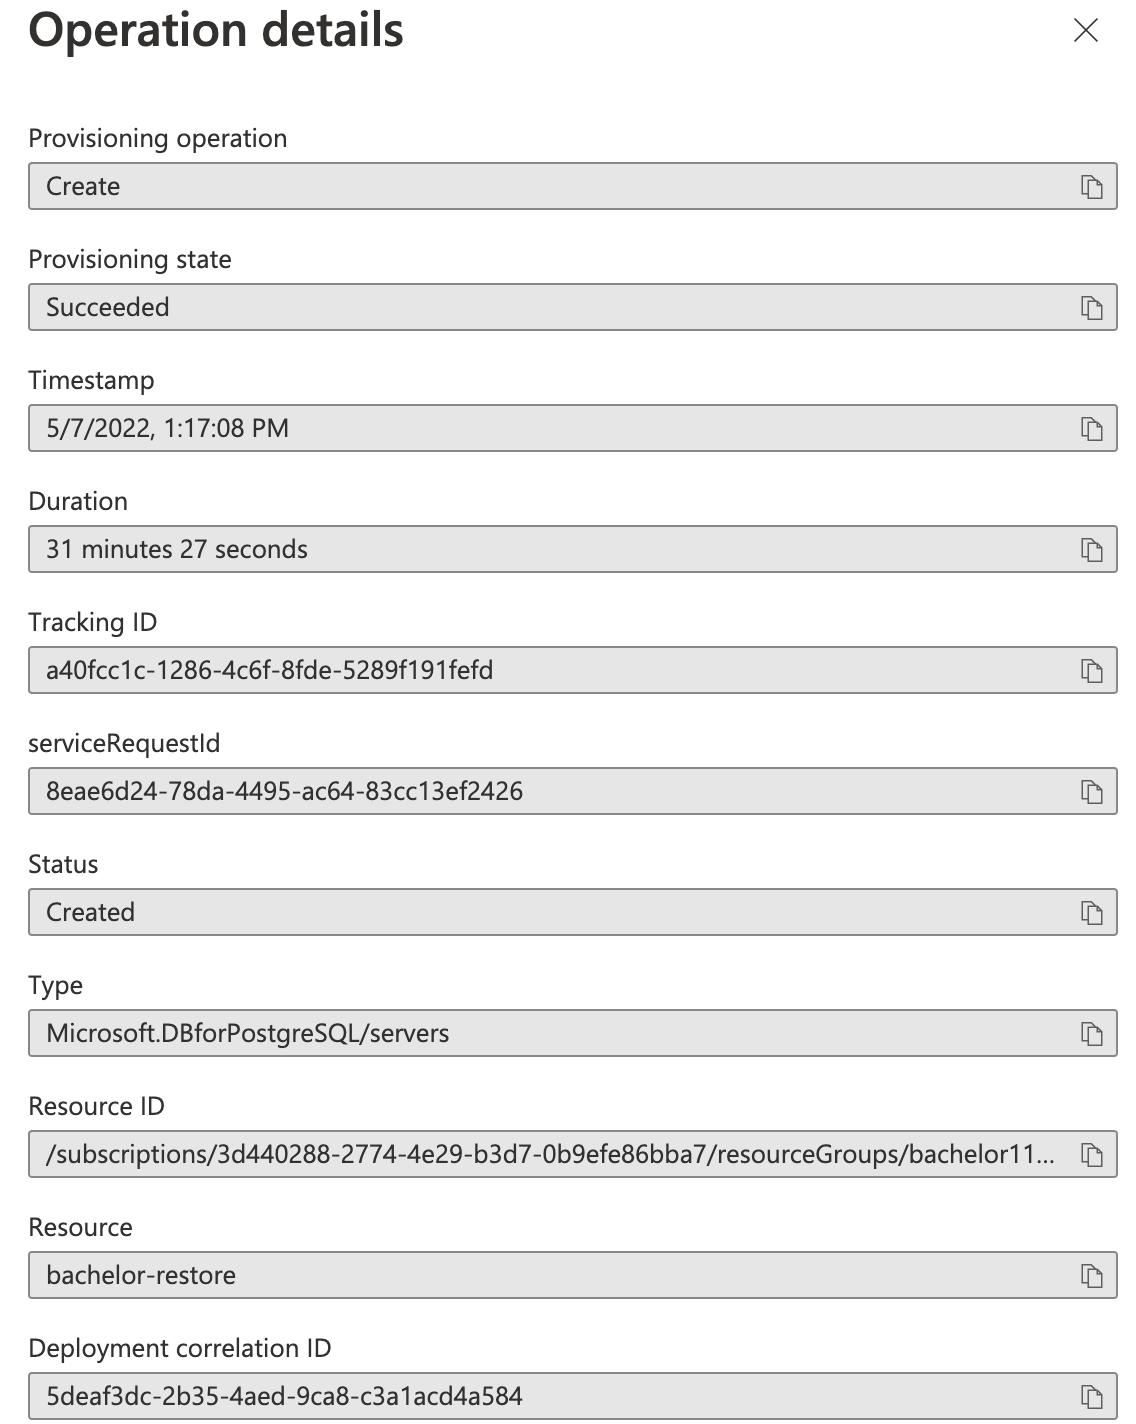
\includegraphics[width=\textwidth, height=15cm]{figures/postgres/PITR-restore.PNG}
    \caption{PITR deploys the database in a newly created server}
    \label{fig:my_label}
\end{figure}
 \section{Setup of test environment for PostgreSQL experiments}

\subsection{Creating test environment for PostgreSQL}\label{pg_setup}
The PostgreSQL instance was 

The Powershell script below is the template for our test environment on the Azure Database for PostgreSQL Single Server.

%A$ecurePassw000rd
\begin{verbatim}
    $Password = Read-Host -Prompt 'Please enter your password' -AsSecureString
    $RGName = "myresourcegroup"
    
    az group create --name $RGName --location northeurope
    
    New-AzPostgreSqlServer `
        -Name bachelorgroup119postgrestest1 `
        -ResourceGroupName $RGName `
        -Sku GP_Gen5_2 `
        -GeoRedundantBackup Enabled `
        -Location northeurope `
        -AdministratorUsername myadmin `
        -AdministratorLoginPassword $Password
\end{verbatim}

\subsection{Data population} \label{pg_populate}
The script below was used to populate the database. 
\begin{minted}[breaklines=true,breakanywhere=true]{python}
import psycopg2
# Connection string information
host = "bachelor119-performance.postgres.database.azure.com"
dbname = "postgres"
user = "bachelor119@bachelor119-performance"
password = "performance-test1"
sslmode = "require"
# Connection string constructed
conn_string = "host={0} user={1} dbname={2} password={3} sslmode={4}".format(host, user, dbname, password, sslmode)
conn = psycopg2.connect(conn_string) 
cursor = conn.cursor()
# Check for duplicate tables
cursor.execute("DROP TABLE IF EXISTS inventory;")
# Create table
cursor.execute("CREATE TABLE inventory (id serial PRIMARY KEY, one BIGINT, two BIGINT, three BIGINT);")
# Insert some data into the table
cursor.execute("INSERT INTO inventory (one, two, three) SELECT generate_series(1, 90000000), generate_series(1, 90000000), generate_series(1, 90000000);")
# Resolve connection
conn.commit()
cursor.close()
conn.close()
\end{minted}

\subsection{Postgres: Azure backup setup}
\label{pg_azurebackup}

In order to back up a postgres server with Azure Backup the first step is to click the "Backup"-option on top of the "Backup instances"-blade inside the Backup Vault.
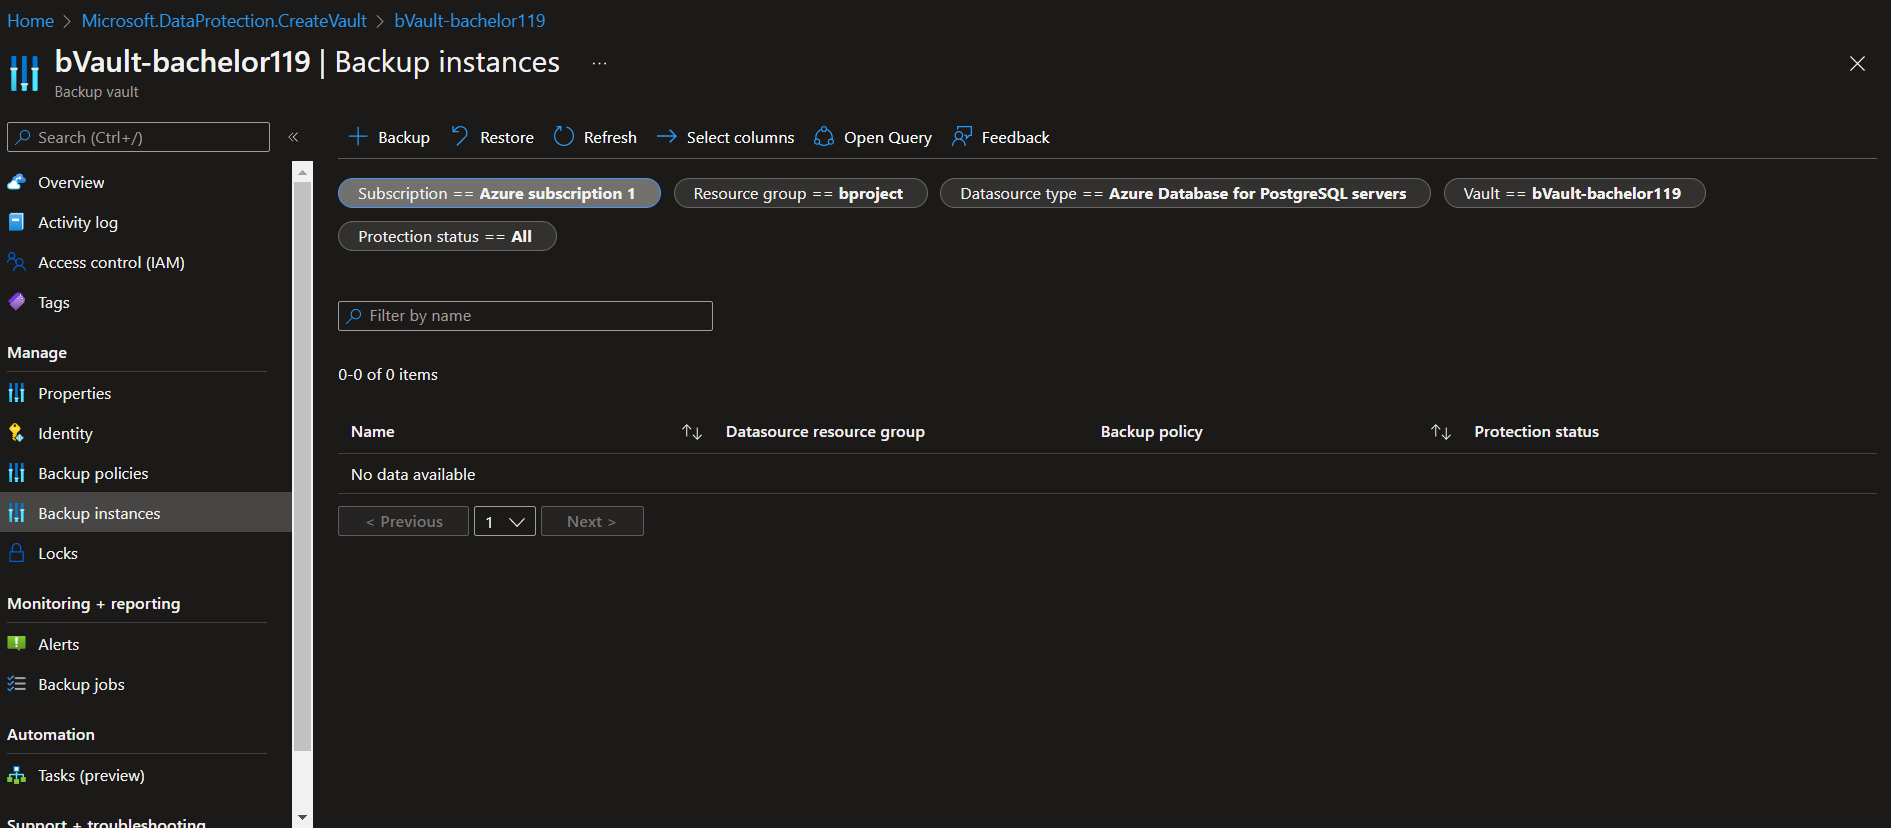
\includegraphics[width=15cm, keepaspectratio]{figures/postgresaasmund/2.PNG}

In the following wizard each organisation must select the options that suit their needs, but importantly it requires the creation of a backup policy. In our example the policy backs up weekly and retains backups for three months. 

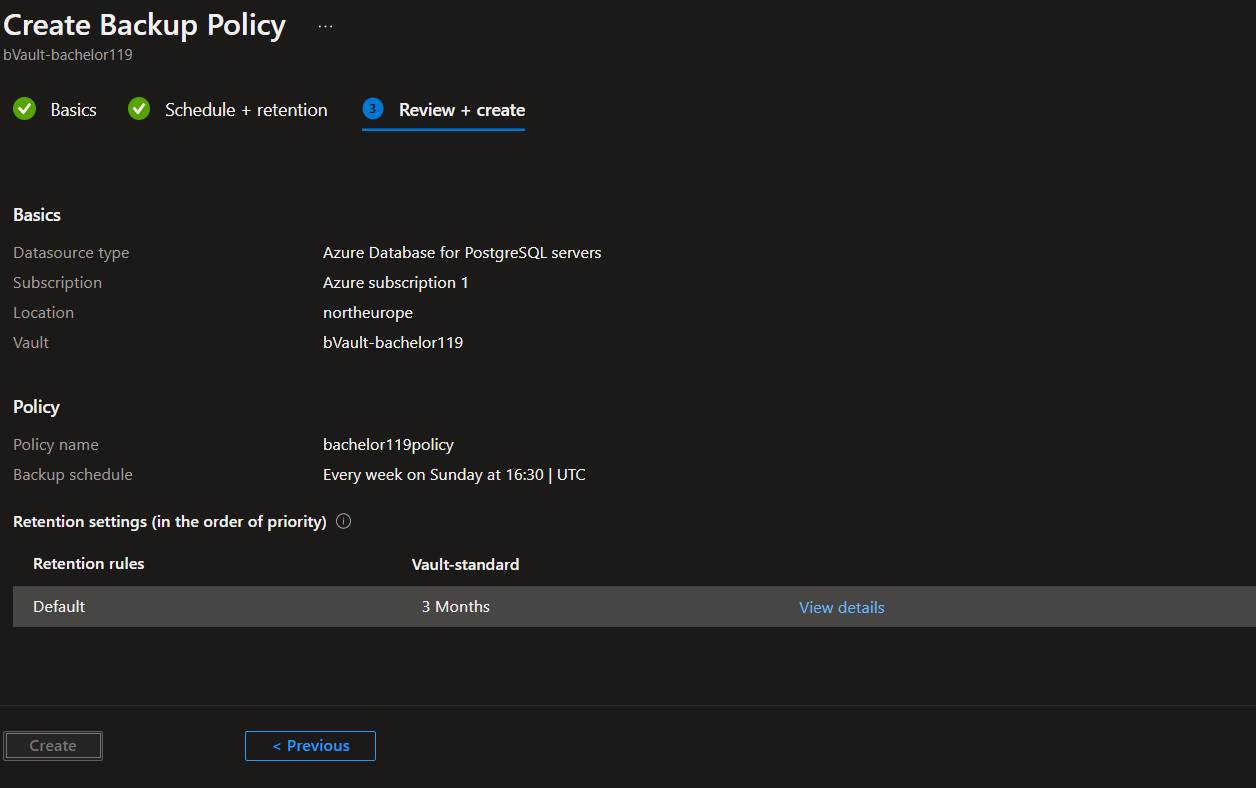
\includegraphics[width=15cm, keepaspectratio]{figures/postgresaasmund/3.PNG}

Additionally when backing up managed postgres servers, we can select which databases to back up. Here we have chosen the standard postgres-database inside the instance, but had we had others we could have chosen them as well. 

When selecting the database we must also give the secret that is required to connect to the database. This can be given as an object i a key vault, as we have done here:

This secret is simply the connection string from the database instance. 

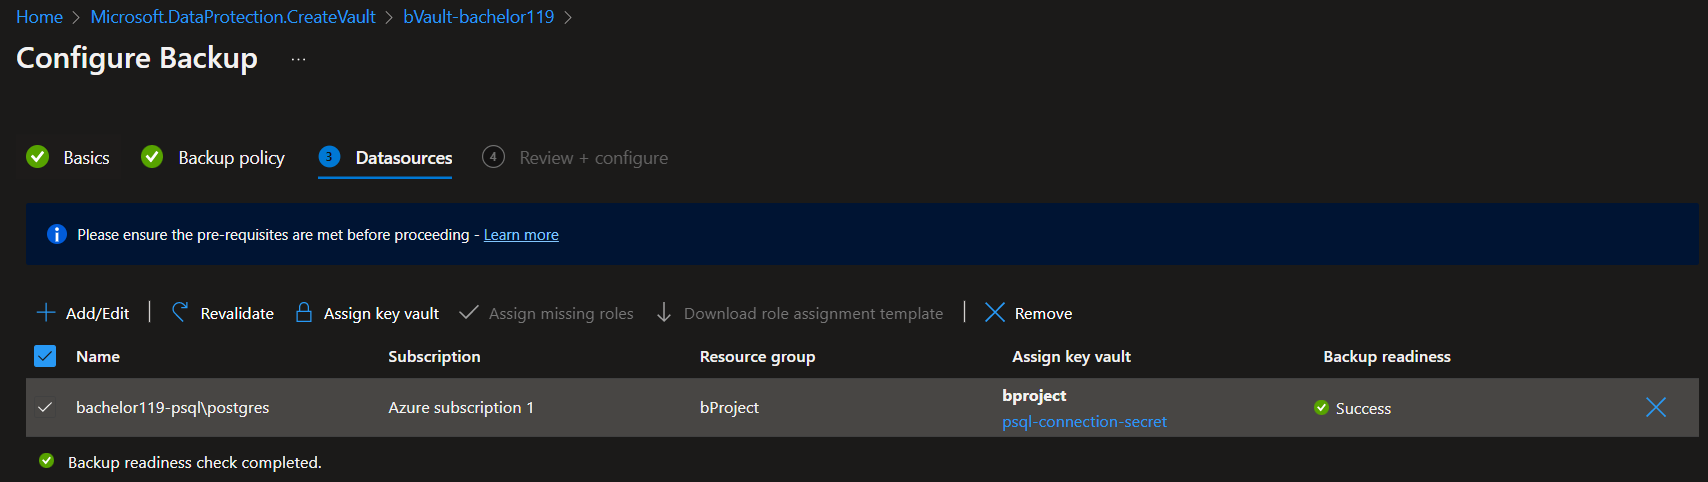
\includegraphics[width=15cm, keepaspectratio]{figures/postgresaasmund/4.PNG}


Finally we have the option to review our options, and if we are happy with these we can create the backup instance. 

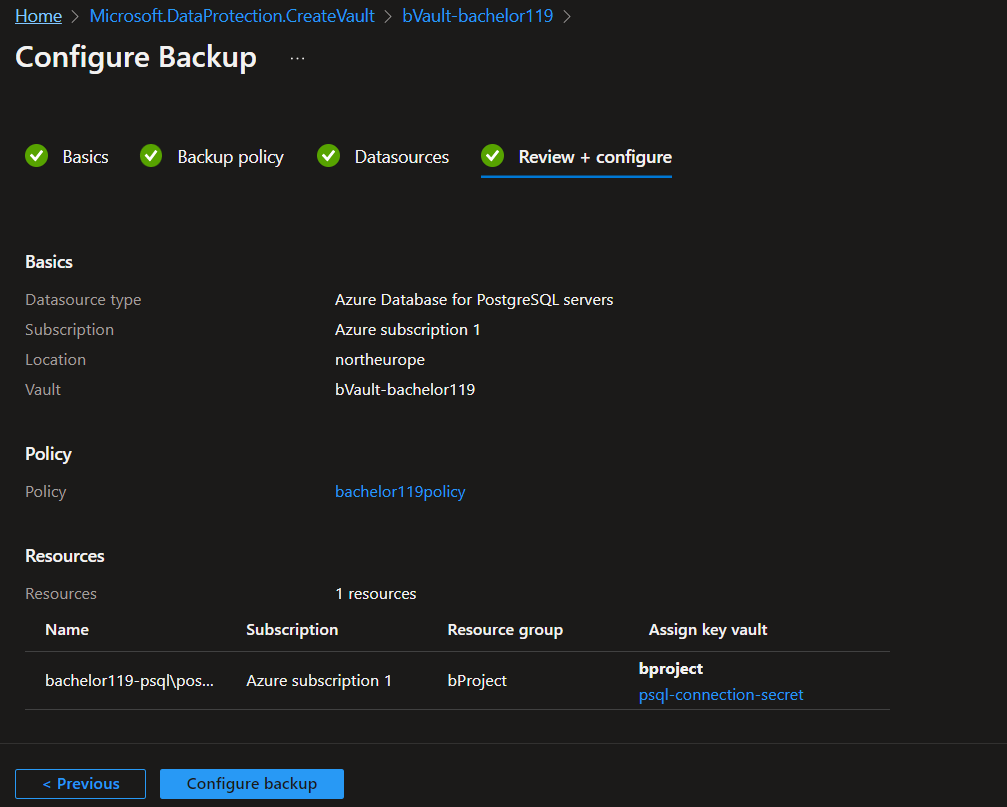
\includegraphics[width=15cm, keepaspectratio]{figures/postgresaasmund/5.PNG}

Immediately after creation the backup instance have not started a backup, and it will not back up the database until we tell it to, or the policy determines that it shall. As shown no backups are completed:

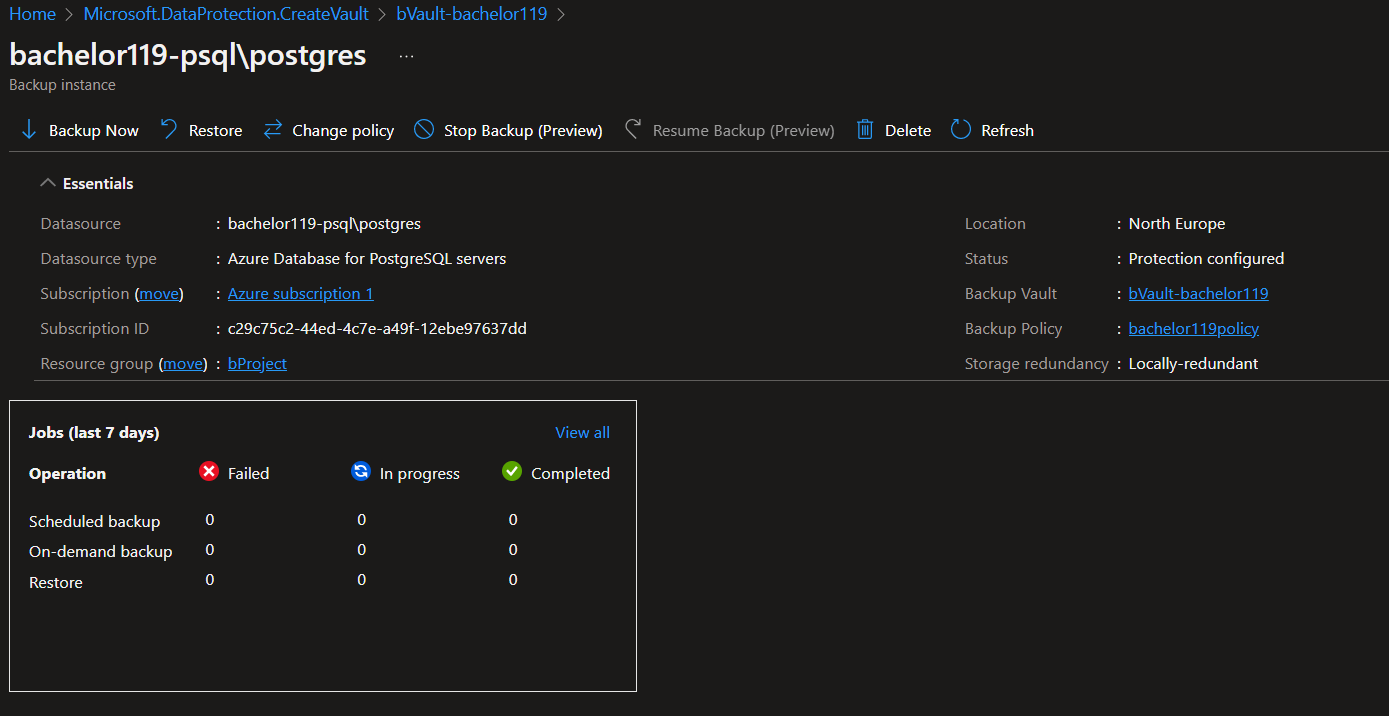
\includegraphics[width=15cm, keepaspectratio]{figures/postgresaasmund/6.PNG}

If we press "back up now" and let it run to completion, we have one completed backup however:

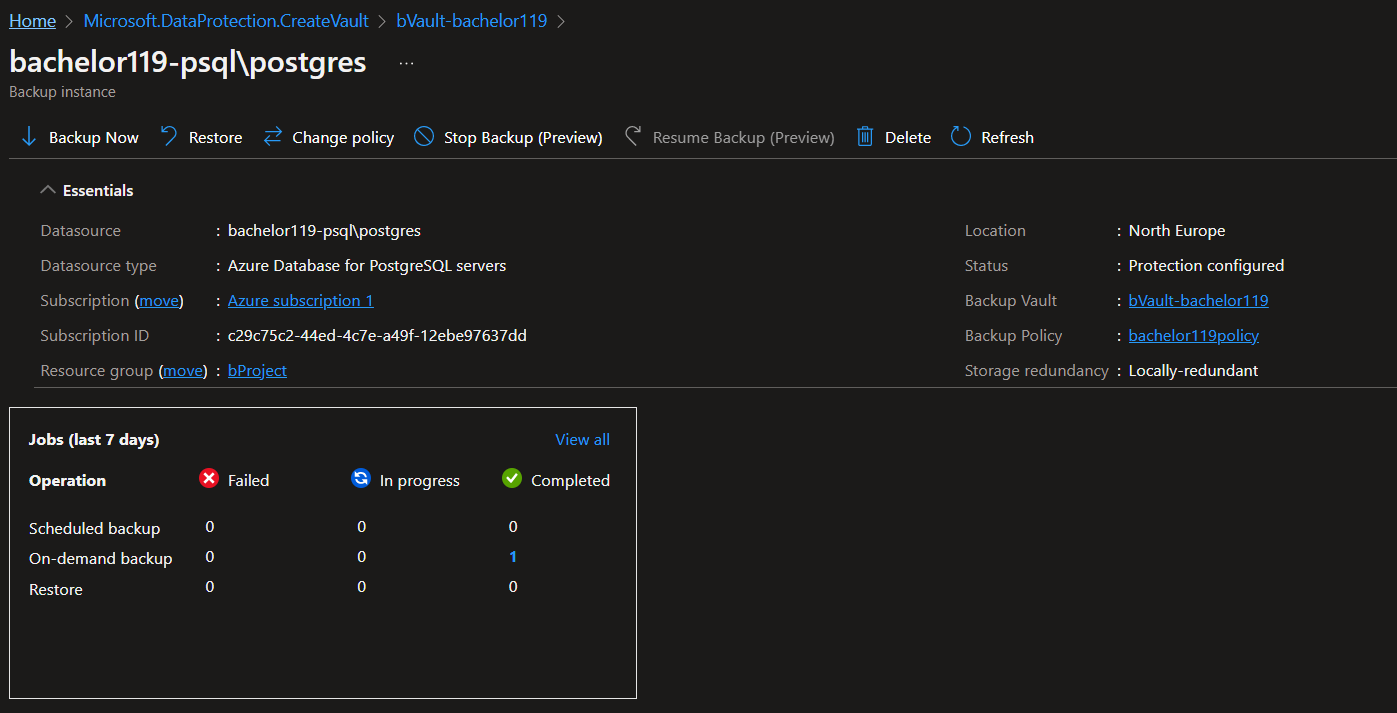
\includegraphics[width=15cm, keepaspectratio]{figures/postgresaasmund/8.PNG}
\label{app_pg_s1e2}
 \section{Postgres: Restoring from PITR}
\label{app_pg_s1e1}

In this experiment we simluated data loss in a postgres database and restored the data with Point-in-time-Restore. 

Given that an attacker encrypts data files in a database in a ransomware attack, we assume complete data loss in the database. This can be simulated with a database (consisting of a single table) being dropped. This is because the security measures designed to mitigate such an attack work the same regardless of the state of the database.

\begin{figure}[h]
    \centering
    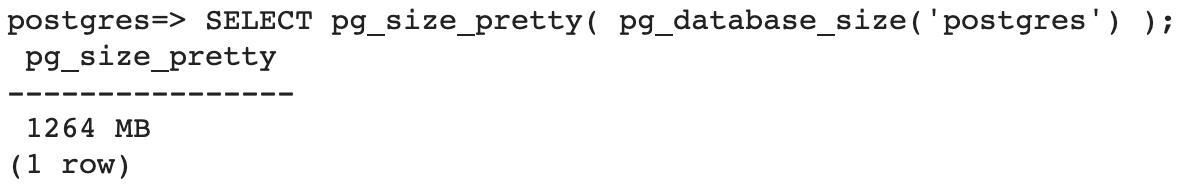
\includegraphics[width=\textwidth]{figures/postgres/postgres-1GB.png}
    \caption{The size of the inventory table}
    \label{fig:my_label}
\end{figure}

\begin{figure}[h]
    \centering
    \includegraphics[scale=0.75]{figures/postgres/drop_table.png}
    \caption{Dropping the table}
    \label{fig:my_label}
\end{figure}

\begin{figure}[h]
    \centering
    \includegraphics[width=\textwidth]{figures/postgres/postgres_size_post.png}
    \caption{The size of the inventory table after dropped table}
    \label{fig:my_label}
\end{figure}


The first security measure is also the simplest solution Azure provides for postgres databases: Point-in-time Restore (PITR). Though there are multiple ways to back up our database.

A point-in-time restore allows the database to be reverted back to a previous state where data has not been tampered with. The user specifies a point in time at which a copy of the database is made and used in the creation of a new managed database server. Such an operation is demonstrated in the following deployment of a restoration database.

\begin{figure}[H]
    \centering
    \includegraphics[width=\textwidth]{figures/postgres/restore_database.png}
    \caption{The restore operation took 31 minutes 27 seconds to complete}
    \label{fig:my_label}
\end{figure}

%This method is especially useful in cases of slow encryption that has been going on for a longer time before being detected.
%This is due to the option of salvaging the  encrypted parts of the database by restoring into a previous unencrypted state and setting together the puzzle pieces of the restored and the live database. 
This way one can recover to the most updated version of the database possible while removing all remnants of malicious activity.
%The estimated time of recovery depends on several factors including the database sizes, the transaction log size, the network bandwidth, and the total number of databases recovering in the same region at the same time. The recovery time varies depending on the the last data backup and the amount of recovery needs to be performed. It is usually less than 12 hours.

The policy for backup retention is dependent on the size of the server. Since we have a 7-day retention period set on the server and the server is no more than 4 TB the backup storage will retain 2 full backups, as well differential backups along with transaction logs from the point of the last full backup. Further information about how server size affects backup and restore policy can be found in the Azure docs for PostgreSQL single server.

%Servers with up to 16-TB storage will retain the full database snapshot, all the differential snapshots and transaction log backups in last 8 days.
%Another option is using the backup vault.
%Our performance tests show that the backup vault provides a performance boost compared to the point-in-time restore. 
%When RPO is of great importance and the operations of the business require handling hundreds of gigabytes of data the difference can be significant enough to make the vault a better suited solution for dealing with the encryption attack scenario.



 \section{Postgres: Protecting with Azure Backup}
\label{app_pg_s1e2}



\subsection{Restoring from Azure Backup}
The data in our database when performing this test is simply 10000 lines of auto-generated code as shown previously. The result of a "SELECT *"-query is as follows:

\includegraphics[width=.9\linewidth]{figures/postgresaasmund/12.PNG}

To simulate data loss, we lose some data by dropping table inventory. The same query now returns an error:

\includegraphics[width=.9\linewidth]{figures/postgresaasmund/10.PNG}

In order to restore from our backup in Azure Backup, we press the "restore"-button on top of the blade. This gives us the following wizard: 

\includegraphics[width=.9\linewidth]{figures/postgresaasmund/11.PNG}

As shown, we are given the option between restoring files or as a database to a server. In this example we choose to restore as a new database on the same server as before. We name this new database "postgres-restored." The same query as before can now be shown on the restored database:

\includegraphics[width=.9\linewidth]{figures/postgresaasmund/13.PNG}

After restoration we can see the successful job in the backup vault:

\includegraphics[width=.9\linewidth]{figures/postgresaasmund/14.PNG}





 \section{Postgres: Deleting database and restoring from PITR}
\label{app_pg_s2e1}



\begin{figure}[H]
    \centering
    \includegraphics[width=\textwidth]{figures/postgres/delete_server.png}
    \caption{JSON output of the delete operation}
    \label{fig:my_label}
\end{figure}

However, this is a form of soft delete since the Azure backup ensures that it is possible to redeploy the server after deletion within the retention period of said server.
In addition, when creating the server the property of "createMode" can be set to "PointInTimeRestore". This can be done through the REST API endpoint for creating servers, where the resource ID of the deleted server has to be included in the request body. 
The resource ID of the deleted server can be found in the JSON file of the delete operation that should be stored in the Azure portal activity log. Below we demonstrate the recovery of the server. 
This way we establish that a server that was encrypted and then deleted still has the ability to fully recover to an operational pre-encryption state.

\begin{figure}[H]
    \centering
    \includegraphics[width=\textwidth]{figures/postgres/recover_deleted_server.png}
    \caption{Summary of the API call}
    \label{fig:my_label}
\end{figure}

\begin{figure}[H]
    \centering
    \includegraphics[width=\textwidth]{figures/postgres/scenario2_restored.png}
    \caption{Server created and database restored}
    \label{fig:my_label}
\end{figure}

 \section{Postgres: Enabling alerts for Backup vault instance deletion}
\label{app_pg_s2e2}

The following template shows how an alert for deleted backup instances can be created. Worth noting that the only supported scope is for the whole subscription, and not a single resource group or Backup vault.

\begin{minted}[breaklines=true,breakanywhere=true]{powershell}
{
    "$schema": "https://schema.management.azure.com/schemas/2019-04-01/deploymentTemplate.json#",
    "contentVersion": "1.0.0.0",
    "parameters": {
        "activityLogAlerts_Deleted_backup_name": {
            "defaultValue": "Deleted backup",
            "type": "String"
        },
        "actiongroups_backup_deletion_notification_externalid": {
            "defaultValue": "/subscriptions/c29c75c2-44ed-4c7e-a49f-12ebe97637dd/resourceGroups/aasmunhs/providers/microsoft.insights/actiongroups/backup deletion notification",
            "type": "String"
        }
    },
    "variables": {},
    "resources": [
        {
            "type": "microsoft.insights/activityLogAlerts",
            "apiVersion": "2020-10-01",
            "name": "[parameters('activityLogAlerts_Deleted_backup_name')]",
            "location": "Global",
            "properties": {
                "scopes": [
                    "/subscriptions/c29c75c2-44ed-4c7e-a49f-12ebe97637dd"
                ],
                "condition": {
                    "allOf": [
                        {
                            "field": "category",
                            "equals": "Administrative"
                        },
                        {
                            "field": "operationName",
                            "equals": "Microsoft.DataProtection/backupVaults/backupInstances/delete"
                        },
                        {
                            "field": "level",
                            "containsAny": [
                                "informational"
                            ]
                        },
                        {
                            "field": "status",
                            "containsAny": [
                                "succeeded"
                            ]
                        }
                    ]
                },
                "actions": {
                    "actionGroups": [
                        {
                            "actionGroupId": "[parameters('actiongroups_backup_deletion_notification_externalid')]",
                            "webhookProperties": {}
                        }
                    ]
                },
                "enabled": true
            }
        }
    ]
}
\end{minted}

As shown, notification type can be modified in the action group:

\includegraphics[width=.9\linewidth]{figures/postgresaasmund/20.PNG}

When deleting a postgres-backup instance the following email was sent:


\begin{minted}[breaklines=true,breakanywhere=true]{text}
Azure Monitor alert 'Deleted backup' was activated for 'bachelor119-psql-postgres-restored-748229ab-ebae-4836-baf5-87bb4150b08c' at May 9, 2022 22:36 UTC
You’re receiving this notification as a member of the BACKUP DELET action group because an Azure Monitor alert was activated.	

Activity log alert	Deleted backup
Time	May 9, 2022 22:36 UTC
Category	Administrative
Operation name	Microsoft.DataProtection/backupVaults/backupInstances/delete
Correlation ID	74d31364-31cb-497a-8c8a-359a81d5b843
Level	Informational
Resource ID	/subscriptions/c29c75c2-44ed-4c7e-a49f-12ebe97637dd/resourceGroups/bProject/providers/Microsoft.DataProtection/backupVaults/bVault-bachelor119/backupInstances/bachelor119-psql-postgres-restored-748229ab-ebae-4836-baf5-87bb4150b08c
Caller	aasmunhs@ntnu.no

Properties	{"eventCategory":"Administrative","entity":"/subscriptions/c29c75c2-44ed-4c7e-a49f-12ebe97637dd/resourceGroups/bProject/providers/Microsoft.DataProtection/backupVaults/bVault-bachelor119/backupInstances/bachelor119-psql-postgres-restored-748229ab-ebae-4836-baf5-87bb4150b08c","message":"Microsoft.DataProtection/backupVaults/backupInstances/delete","hierarchy":"09a10672-822f-4467-a5ba-5bb375967c05/c29c75c2-44ed-4c7e-a49f-12ebe97637dd"}

\end{minted}


% \input{appendices/pg_s2e3} %Don't think this is needed. It is simply "deleting backup data" Unless we have documentation of it??



\end{document}
